\documentclass[twoside]{book}

% Packages required by doxygen
\usepackage{calc}
\usepackage{doxygen}
\usepackage{graphicx}
\usepackage[utf8]{inputenc}
\usepackage{makeidx}
\usepackage{multicol}
\usepackage{multirow}
\usepackage{textcomp}
\usepackage[table]{xcolor}

% Font selection
\usepackage[T1]{fontenc}
\usepackage{mathptmx}
\usepackage[scaled=.90]{helvet}
\usepackage{courier}
\usepackage{amssymb}
\usepackage{sectsty}
\renewcommand{\familydefault}{\sfdefault}
\allsectionsfont{%
  \fontseries{bc}\selectfont%
  \color{darkgray}%
}
\renewcommand{\DoxyLabelFont}{%
  \fontseries{bc}\selectfont%
  \color{darkgray}%
}

% Page & text layout
\usepackage{geometry}
\geometry{%
  a4paper,%
  top=2.5cm,%
  bottom=2.5cm,%
  left=2.5cm,%
  right=2.5cm%
}
\tolerance=750
\hfuzz=15pt
\hbadness=750
\setlength{\emergencystretch}{15pt}
\setlength{\parindent}{0cm}
\setlength{\parskip}{0.2cm}
\makeatletter
\renewcommand{\paragraph}{%
  \@startsection{paragraph}{4}{0ex}{-1.0ex}{1.0ex}{%
    \normalfont\normalsize\bfseries\SS@parafont%
  }%
}
\renewcommand{\subparagraph}{%
  \@startsection{subparagraph}{5}{0ex}{-1.0ex}{1.0ex}{%
    \normalfont\normalsize\bfseries\SS@subparafont%
  }%
}
\makeatother

% Headers & footers
\usepackage{fancyhdr}
\pagestyle{fancyplain}
\fancyhead[LE]{\fancyplain{}{\bfseries\thepage}}
\fancyhead[CE]{\fancyplain{}{}}
\fancyhead[RE]{\fancyplain{}{\bfseries\leftmark}}
\fancyhead[LO]{\fancyplain{}{\bfseries\rightmark}}
\fancyhead[CO]{\fancyplain{}{}}
\fancyhead[RO]{\fancyplain{}{\bfseries\thepage}}
\fancyfoot[LE]{\fancyplain{}{}}
\fancyfoot[CE]{\fancyplain{}{}}
\fancyfoot[RE]{\fancyplain{}{\bfseries\scriptsize Generated on Wed Jun 10 2015 23\-:37\-:21 for '\-Projet\-C++' by Doxygen }}
\fancyfoot[LO]{\fancyplain{}{\bfseries\scriptsize Generated on Wed Jun 10 2015 23\-:37\-:21 for '\-Projet\-C++' by Doxygen }}
\fancyfoot[CO]{\fancyplain{}{}}
\fancyfoot[RO]{\fancyplain{}{}}
\renewcommand{\footrulewidth}{0.4pt}
\renewcommand{\chaptermark}[1]{%
  \markboth{#1}{}%
}
\renewcommand{\sectionmark}[1]{%
  \markright{\thesection\ #1}%
}

% Indices & bibliography
\usepackage{natbib}
\usepackage[titles]{tocloft}
\setcounter{tocdepth}{3}
\setcounter{secnumdepth}{5}
\makeindex

% Hyperlinks (required, but should be loaded last)
\usepackage{ifpdf}
\ifpdf
  \usepackage[pdftex,pagebackref=true]{hyperref}
\else
  \usepackage[ps2pdf,pagebackref=true]{hyperref}
\fi
\hypersetup{%
  colorlinks=true,%
  linkcolor=blue,%
  citecolor=blue,%
  unicode%
}

% Custom commands
\newcommand{\clearemptydoublepage}{%
  \newpage{\pagestyle{empty}\cleardoublepage}%
}


%===== C O N T E N T S =====

\begin{document}

% Titlepage & ToC
\hypersetup{pageanchor=false}
\pagenumbering{roman}
\begin{titlepage}
\vspace*{7cm}
\begin{center}%
{\Large 'Projet\-C++' }\\
\vspace*{1cm}
{\large Generated by Doxygen 1.8.6}\\
\vspace*{0.5cm}
{\small Wed Jun 10 2015 23:37:21}\\
\end{center}
\end{titlepage}
\clearemptydoublepage
\tableofcontents
\clearemptydoublepage
\pagenumbering{arabic}
\hypersetup{pageanchor=true}

%--- Begin generated contents ---
\chapter{Hierarchical Index}
\section{Class Hierarchy}
This inheritance list is sorted roughly, but not completely, alphabetically\-:\begin{DoxyCompactList}
\item \contentsline{section}{Action}{\pageref{classAction}}{}
\begin{DoxyCompactList}
\item \contentsline{section}{Action\-Changement\-Carte}{\pageref{classActionChangementCarte}}{}
\item \contentsline{section}{Action\-Combat}{\pageref{classActionCombat}}{}
\item \contentsline{section}{Action\-Vide}{\pageref{classActionVide}}{}
\end{DoxyCompactList}
\item \contentsline{section}{Arme}{\pageref{classArme}}{}
\begin{DoxyCompactList}
\item \contentsline{section}{Arme\-Chercheuse}{\pageref{classArmeChercheuse}}{}
\item \contentsline{section}{Arme\-Classique}{\pageref{classArmeClassique}}{}
\item \contentsline{section}{Arme\-Croix}{\pageref{classArmeCroix}}{}
\item \contentsline{section}{Arme\-Fatale}{\pageref{classArmeFatale}}{}
\end{DoxyCompactList}
\item \contentsline{section}{Bateau}{\pageref{classBateau}}{}
\item \contentsline{section}{Carte}{\pageref{classCarte}}{}
\item \contentsline{section}{Case}{\pageref{classCase}}{}
\item \contentsline{section}{Cellule}{\pageref{classCellule}}{}
\begin{DoxyCompactList}
\item \contentsline{section}{Cellule\-Accessible}{\pageref{classCelluleAccessible}}{}
\begin{DoxyCompactList}
\item \contentsline{section}{Cellule\-Changement\-Carte}{\pageref{classCelluleChangementCarte}}{}
\item \contentsline{section}{Cellule\-Combat}{\pageref{classCelluleCombat}}{}
\end{DoxyCompactList}
\item \contentsline{section}{Cellule\-Obstacle}{\pageref{classCelluleObstacle}}{}
\end{DoxyCompactList}
\item \contentsline{section}{Combat}{\pageref{classCombat}}{}
\begin{DoxyCompactList}
\item \contentsline{section}{Bataille\-Navale}{\pageref{classBatailleNavale}}{}
\end{DoxyCompactList}
\item \contentsline{section}{Controleur}{\pageref{classControleur}}{}
\item \contentsline{section}{Controleur\-B\-N}{\pageref{classControleurBN}}{}
\item \contentsline{section}{Coordonnees}{\pageref{classCoordonnees}}{}
\item \contentsline{section}{Grille}{\pageref{classGrille}}{}
\item \contentsline{section}{I\-H\-M\-B\-N}{\pageref{classIHMBN}}{}
\item \contentsline{section}{I\-H\-M\-Jeu}{\pageref{classIHMJeu}}{}
\item \contentsline{section}{Inventaire}{\pageref{classInventaire}}{}
\item \contentsline{section}{Jeu}{\pageref{classJeu}}{}
\item \contentsline{section}{Monde}{\pageref{classMonde}}{}
\item \contentsline{section}{Objet}{\pageref{classObjet}}{}
\begin{DoxyCompactList}
\item \contentsline{section}{Badge\-Final}{\pageref{classBadgeFinal}}{}
\end{DoxyCompactList}
\item \contentsline{section}{Personnage}{\pageref{classPersonnage}}{}
\begin{DoxyCompactList}
\item \contentsline{section}{Personnage\-Jouable}{\pageref{classPersonnageJouable}}{}
\begin{DoxyCompactList}
\item \contentsline{section}{Joueur\-Dhumain\-B\-Nia}{\pageref{classJoueurDhumainBNia}}{}
\item \contentsline{section}{Joueur\-Humain}{\pageref{classJoueurHumain}}{}
\end{DoxyCompactList}
\item \contentsline{section}{Personnage\-Non\-Jouable}{\pageref{classPersonnageNonJouable}}{}
\begin{DoxyCompactList}
\item \contentsline{section}{Joueur\-I\-A}{\pageref{classJoueurIA}}{}
\item \contentsline{section}{Joueur\-I\-A\-Avance}{\pageref{classJoueurIAAvance}}{}
\item \contentsline{section}{Joueur\-I\-A\-Cheate}{\pageref{classJoueurIACheate}}{}
\end{DoxyCompactList}
\end{DoxyCompactList}
\item \contentsline{section}{Personnage\-B\-N}{\pageref{classPersonnageBN}}{}
\begin{DoxyCompactList}
\item \contentsline{section}{Personnage\-B\-N\-Humain}{\pageref{classPersonnageBNHumain}}{}
\begin{DoxyCompactList}
\item \contentsline{section}{Joueur\-Humain}{\pageref{classJoueurHumain}}{}
\end{DoxyCompactList}
\item \contentsline{section}{Personnage\-B\-N\-I\-A}{\pageref{classPersonnageBNIA}}{}
\begin{DoxyCompactList}
\item \contentsline{section}{Joueur\-Dhumain\-B\-Nia}{\pageref{classJoueurDhumainBNia}}{}
\item \contentsline{section}{Joueur\-I\-A}{\pageref{classJoueurIA}}{}
\end{DoxyCompactList}
\item \contentsline{section}{Personnage\-B\-N\-I\-A\-Avance}{\pageref{classPersonnageBNIAAvance}}{}
\begin{DoxyCompactList}
\item \contentsline{section}{Joueur\-I\-A\-Avance}{\pageref{classJoueurIAAvance}}{}
\end{DoxyCompactList}
\item \contentsline{section}{Personnage\-B\-N\-I\-A\-Cheate}{\pageref{classPersonnageBNIACheate}}{}
\begin{DoxyCompactList}
\item \contentsline{section}{Joueur\-I\-A\-Cheate}{\pageref{classJoueurIACheate}}{}
\end{DoxyCompactList}
\end{DoxyCompactList}
\item \contentsline{section}{Taille\-Grille}{\pageref{classTailleGrille}}{}
\end{DoxyCompactList}

\chapter{Class Index}
\section{Class List}
Here are the classes, structs, unions and interfaces with brief descriptions\-:\begin{DoxyCompactList}
\item\contentsline{section}{\hyperlink{classAction}{Action} \\*Gestion actions }{\pageref{classAction}}{}
\item\contentsline{section}{\hyperlink{classActionChangementCarte}{Action\-Changement\-Carte} \\*Gestion changement de carte }{\pageref{classActionChangementCarte}}{}
\item\contentsline{section}{\hyperlink{classActionCombat}{Action\-Combat} \\*Gestion lancement du combat }{\pageref{classActionCombat}}{}
\item\contentsline{section}{\hyperlink{classActionVide}{Action\-Vide} \\*Lance une action vide }{\pageref{classActionVide}}{}
\item\contentsline{section}{\hyperlink{classArme}{Arme} \\*Gestion de l'arme }{\pageref{classArme}}{}
\item\contentsline{section}{\hyperlink{classArmeChercheuse}{Arme\-Chercheuse} \\*Gestion de l'\hyperlink{classArme}{Arme} Chercheuse }{\pageref{classArmeChercheuse}}{}
\item\contentsline{section}{\hyperlink{classArmeClassique}{Arme\-Classique} \\*Gestion de l'\hyperlink{classArme}{Arme} Classique }{\pageref{classArmeClassique}}{}
\item\contentsline{section}{\hyperlink{classArmeCroix}{Arme\-Croix} \\*Gestion de l'\hyperlink{classArme}{Arme} Croix }{\pageref{classArmeCroix}}{}
\item\contentsline{section}{\hyperlink{classArmeFatale}{Arme\-Fatale} \\*Gestion de l'\hyperlink{classArme}{Arme} Fatale }{\pageref{classArmeFatale}}{}
\item\contentsline{section}{\hyperlink{classBadgeFinal}{Badge\-Final} \\*Gestion des badges finaux }{\pageref{classBadgeFinal}}{}
\item\contentsline{section}{\hyperlink{classBatailleNavale}{Bataille\-Navale} \\*Classe combat bataille navale }{\pageref{classBatailleNavale}}{}
\item\contentsline{section}{\hyperlink{classBateau}{Bateau} \\*Classe représentant bateaux }{\pageref{classBateau}}{}
\item\contentsline{section}{\hyperlink{classCarte}{Carte} \\*Classe représentant une carte }{\pageref{classCarte}}{}
\item\contentsline{section}{\hyperlink{classCase}{Case} \\*La \hyperlink{classCase}{Case} est comprise dans une grille de Bataille Navale }{\pageref{classCase}}{}
\item\contentsline{section}{\hyperlink{classCellule}{Cellule} \\*\hyperlink{classCellule}{Cellule} composant les Zones du \hyperlink{classMonde}{Monde} où le joueur se déplace }{\pageref{classCellule}}{}
\item\contentsline{section}{\hyperlink{classCelluleAccessible}{Cellule\-Accessible} \\*Classe représentant les cellules du monde auquelles les personnages peuvent accéder }{\pageref{classCelluleAccessible}}{}
\item\contentsline{section}{\hyperlink{classCelluleChangementCarte}{Cellule\-Changement\-Carte} \\*\hyperlink{classCelluleAccessible}{Cellule\-Accessible} permettant d'engager un Changement\-Carte }{\pageref{classCelluleChangementCarte}}{}
\item\contentsline{section}{\hyperlink{classCelluleCombat}{Cellule\-Combat} \\*\hyperlink{classCelluleAccessible}{Cellule\-Accessible} permettant d'engager un \hyperlink{classCombat}{Combat} }{\pageref{classCelluleCombat}}{}
\item\contentsline{section}{\hyperlink{classCelluleObstacle}{Cellule\-Obstacle} \\*\hyperlink{classCellule}{Cellule} contenant un obstacle }{\pageref{classCelluleObstacle}}{}
\item\contentsline{section}{\hyperlink{classCombat}{Combat} \\*\hyperlink{classCombat}{Combat} à deux joueurs }{\pageref{classCombat}}{}
\item\contentsline{section}{\hyperlink{classControleur}{Controleur} \\*\hyperlink{classControleur}{Controleur} de notre partie }{\pageref{classControleur}}{}
\item\contentsline{section}{\hyperlink{classControleurBN}{Controleur\-B\-N} \\*\hyperlink{classControleur}{Controleur} de notre B\-N }{\pageref{classControleurBN}}{}
\item\contentsline{section}{\hyperlink{classCoordonnees}{Coordonnees} \\*\hyperlink{classCoordonnees}{Coordonnees} sur une carte }{\pageref{classCoordonnees}}{}
\item\contentsline{section}{\hyperlink{classGrille}{Grille} \\*\hyperlink{classGrille}{Grille} de bataille navale }{\pageref{classGrille}}{}
\item\contentsline{section}{\hyperlink{classIHMBN}{I\-H\-M\-B\-N} \\*I\-H\-M pour Bataille Navale }{\pageref{classIHMBN}}{}
\item\contentsline{section}{\hyperlink{classIHMJeu}{I\-H\-M\-Jeu} \\*Classe representant l'I\-H\-M gerant le jeu }{\pageref{classIHMJeu}}{}
\item\contentsline{section}{\hyperlink{classInventaire}{Inventaire} \\*Classe représentant l'inventaire }{\pageref{classInventaire}}{}
\item\contentsline{section}{\hyperlink{classJeu}{Jeu} \\*Déplacement sur la carte }{\pageref{classJeu}}{}
\item\contentsline{section}{\hyperlink{classJoueurDhumainBNia}{Joueur\-Dhumain\-B\-Nia} \\*Classe définissant un joueur I\-A }{\pageref{classJoueurDhumainBNia}}{}
\item\contentsline{section}{\hyperlink{classJoueurHumain}{Joueur\-Humain} \\*Classe définissant un joueur humain }{\pageref{classJoueurHumain}}{}
\item\contentsline{section}{\hyperlink{classJoueurIA}{Joueur\-I\-A} \\*Classe définissant un joueur I\-A }{\pageref{classJoueurIA}}{}
\item\contentsline{section}{\hyperlink{classJoueurIAAvance}{Joueur\-I\-A\-Avance} \\*Classe définissant un joueur I\-A }{\pageref{classJoueurIAAvance}}{}
\item\contentsline{section}{\hyperlink{classJoueurIACheate}{Joueur\-I\-A\-Cheate} \\*Classe définissant un joueur I\-A }{\pageref{classJoueurIACheate}}{}
\item\contentsline{section}{\hyperlink{classMonde}{Monde} \\*Classe définissant un monde }{\pageref{classMonde}}{}
\item\contentsline{section}{\hyperlink{classObjet}{Objet} \\*Gestion des objets }{\pageref{classObjet}}{}
\item\contentsline{section}{\hyperlink{classPersonnage}{Personnage} \\*Classe définissant un personnage }{\pageref{classPersonnage}}{}
\item\contentsline{section}{\hyperlink{classPersonnageBN}{Personnage\-B\-N} \\*\hyperlink{classPersonnage}{Personnage} pouvant jouer au combat\-: \hyperlink{classBatailleNavale}{Bataille\-Navale} }{\pageref{classPersonnageBN}}{}
\item\contentsline{section}{\hyperlink{classPersonnageBNHumain}{Personnage\-B\-N\-Humain} \\*\hyperlink{classPersonnage}{Personnage} de bataille navale associé au joueur }{\pageref{classPersonnageBNHumain}}{}
\item\contentsline{section}{\hyperlink{classPersonnageBNIA}{Personnage\-B\-N\-I\-A} \\*Personnages de bataille navale dotés d'une intelligence artificielle }{\pageref{classPersonnageBNIA}}{}
\item\contentsline{section}{\hyperlink{classPersonnageBNIAAvance}{Personnage\-B\-N\-I\-A\-Avance} \\*Personnages de bataille navale dotés d'une intelligence artificielle }{\pageref{classPersonnageBNIAAvance}}{}
\item\contentsline{section}{\hyperlink{classPersonnageBNIACheate}{Personnage\-B\-N\-I\-A\-Cheate} \\*Personnages de bataille navale dotés d'une intelligence artificielle }{\pageref{classPersonnageBNIACheate}}{}
\item\contentsline{section}{\hyperlink{classPersonnageJouable}{Personnage\-Jouable} \\*Classe definissant un personnage jouable }{\pageref{classPersonnageJouable}}{}
\item\contentsline{section}{\hyperlink{classPersonnageNonJouable}{Personnage\-Non\-Jouable} \\*Classe définissant un personnage non jouable }{\pageref{classPersonnageNonJouable}}{}
\item\contentsline{section}{\hyperlink{classTailleGrille}{Taille\-Grille} \\*Clase representant la taille de la \hyperlink{classGrille}{Grille} }{\pageref{classTailleGrille}}{}
\end{DoxyCompactList}

\chapter{File Index}
\section{File List}
Here is a list of all documented files with brief descriptions\-:\begin{DoxyCompactList}
\item\contentsline{section}{/home/damien/\-Bureau/projetcpp\-\_\-gm42/source/src/\hyperlink{Action_8hpp}{Action.\-hpp} \\*Lance l'action associée à la case }{\pageref{Action_8hpp}}{}
\item\contentsline{section}{/home/damien/\-Bureau/projetcpp\-\_\-gm42/source/src/\hyperlink{ActionChangementCarte_8hpp}{Action\-Changement\-Carte.\-hpp} \\*Change la carte si besoin }{\pageref{ActionChangementCarte_8hpp}}{}
\item\contentsline{section}{/home/damien/\-Bureau/projetcpp\-\_\-gm42/source/src/\hyperlink{ActionCombat_8hpp}{Action\-Combat.\-hpp} \\*Lance un combat quand besoin }{\pageref{ActionCombat_8hpp}}{}
\item\contentsline{section}{/home/damien/\-Bureau/projetcpp\-\_\-gm42/source/src/\hyperlink{ActionVide_8hpp}{Action\-Vide.\-hpp} \\*\hyperlink{classAction}{Action} vide }{\pageref{ActionVide_8hpp}}{}
\item\contentsline{section}{/home/damien/\-Bureau/projetcpp\-\_\-gm42/source/src/\hyperlink{Arme_8hpp}{Arme.\-hpp} \\*Gestion des armes }{\pageref{Arme_8hpp}}{}
\item\contentsline{section}{/home/damien/\-Bureau/projetcpp\-\_\-gm42/source/src/\hyperlink{ArmeChercheuse_8hpp}{Arme\-Chercheuse.\-hpp} \\*Gestion de l'\hyperlink{classArme}{Arme} Chercheuse }{\pageref{ArmeChercheuse_8hpp}}{}
\item\contentsline{section}{/home/damien/\-Bureau/projetcpp\-\_\-gm42/source/src/\hyperlink{ArmeClassique_8hpp}{Arme\-Classique.\-hpp} \\*Gestion de l'\hyperlink{classArme}{Arme} Classique }{\pageref{ArmeClassique_8hpp}}{}
\item\contentsline{section}{/home/damien/\-Bureau/projetcpp\-\_\-gm42/source/src/\hyperlink{ArmeCroix_8hpp}{Arme\-Croix.\-hpp} \\*Gestion de l'\hyperlink{classArme}{Arme} Croix }{\pageref{ArmeCroix_8hpp}}{}
\item\contentsline{section}{/home/damien/\-Bureau/projetcpp\-\_\-gm42/source/src/\hyperlink{ArmeFatale_8hpp}{Arme\-Fatale.\-hpp} \\*Gestion de l'\hyperlink{classArme}{Arme} Classique }{\pageref{ArmeFatale_8hpp}}{}
\item\contentsline{section}{/home/damien/\-Bureau/projetcpp\-\_\-gm42/source/src/\hyperlink{BadgeFinal_8hpp}{Badge\-Final.\-hpp} \\*Fichier de la classe \hyperlink{classBadgeFinal}{Badge\-Final} }{\pageref{BadgeFinal_8hpp}}{}
\item\contentsline{section}{/home/damien/\-Bureau/projetcpp\-\_\-gm42/source/src/\hyperlink{BatailleNavale_8hpp}{Bataille\-Navale.\-hpp} \\*Gestion d'un combat bataille navale }{\pageref{BatailleNavale_8hpp}}{}
\item\contentsline{section}{/home/damien/\-Bureau/projetcpp\-\_\-gm42/source/src/\hyperlink{Bateau_8hpp}{Bateau.\-hpp} \\*Définition bateaux bataille navale }{\pageref{Bateau_8hpp}}{}
\item\contentsline{section}{/home/damien/\-Bureau/projetcpp\-\_\-gm42/source/src/\hyperlink{Carte_8hpp}{Carte.\-hpp} \\*Représentant carte }{\pageref{Carte_8hpp}}{}
\item\contentsline{section}{/home/damien/\-Bureau/projetcpp\-\_\-gm42/source/src/\hyperlink{Case_8hpp}{Case.\-hpp} \\*Fichier contenant la classe \hyperlink{classCase}{Case} }{\pageref{Case_8hpp}}{}
\item\contentsline{section}{/home/damien/\-Bureau/projetcpp\-\_\-gm42/source/src/\hyperlink{Cellule_8hpp}{Cellule.\-hpp} \\*Fichier contenant la classe \hyperlink{classCellule}{Cellule} }{\pageref{Cellule_8hpp}}{}
\item\contentsline{section}{/home/damien/\-Bureau/projetcpp\-\_\-gm42/source/src/\hyperlink{CelluleAccessible_8hpp}{Cellule\-Accessible.\-hpp} \\*Fichier contenant la classe \hyperlink{classCelluleAccessible}{Cellule\-Accessible} }{\pageref{CelluleAccessible_8hpp}}{}
\item\contentsline{section}{/home/damien/\-Bureau/projetcpp\-\_\-gm42/source/src/\hyperlink{CelluleChangementCarte_8hpp}{Cellule\-Changement\-Carte.\-hpp} \\*Fichier contenant le classe \hyperlink{classCelluleChangementCarte}{Cellule\-Changement\-Carte} }{\pageref{CelluleChangementCarte_8hpp}}{}
\item\contentsline{section}{/home/damien/\-Bureau/projetcpp\-\_\-gm42/source/src/\hyperlink{CelluleCombat_8hpp}{Cellule\-Combat.\-hpp} \\*Fichier contenant le classe \hyperlink{classCelluleCombat}{Cellule\-Combat} }{\pageref{CelluleCombat_8hpp}}{}
\item\contentsline{section}{/home/damien/\-Bureau/projetcpp\-\_\-gm42/source/src/\hyperlink{CelluleObstacle_8hpp}{Cellule\-Obstacle.\-hpp} \\*\hyperlink{classCellule}{Cellule} contenant un obstacle }{\pageref{CelluleObstacle_8hpp}}{}
\item\contentsline{section}{/home/damien/\-Bureau/projetcpp\-\_\-gm42/source/src/\hyperlink{Combat_8hpp}{Combat.\-hpp} \\*Gestion d'un combat à deux joueurs }{\pageref{Combat_8hpp}}{}
\item\contentsline{section}{/home/damien/\-Bureau/projetcpp\-\_\-gm42/source/src/\hyperlink{Controleur_8hpp}{Controleur.\-hpp} \\*\hyperlink{classControleur}{Controleur} de notre jeu }{\pageref{Controleur_8hpp}}{}
\item\contentsline{section}{/home/damien/\-Bureau/projetcpp\-\_\-gm42/source/src/\hyperlink{ControleurBN_8hpp}{Controleur\-B\-N.\-hpp} \\*\hyperlink{classControleurBN}{Controleur\-B\-N} de notre jeu }{\pageref{ControleurBN_8hpp}}{}
\item\contentsline{section}{/home/damien/\-Bureau/projetcpp\-\_\-gm42/source/src/\hyperlink{Coordonnees_8hpp}{Coordonnees.\-hpp} \\*Coordonnées sur une carte }{\pageref{Coordonnees_8hpp}}{}
\item\contentsline{section}{/home/damien/\-Bureau/projetcpp\-\_\-gm42/source/src/\hyperlink{Grille_8hpp}{Grille.\-hpp} \\*Fichier contenant la classe \hyperlink{classGrille}{Grille} }{\pageref{Grille_8hpp}}{}
\item\contentsline{section}{/home/damien/\-Bureau/projetcpp\-\_\-gm42/source/src/\hyperlink{IHMBN_8hpp}{I\-H\-M\-B\-N.\-hpp} \\*Fichier contenant la classe \hyperlink{classIHMBN}{I\-H\-M\-B\-N} }{\pageref{IHMBN_8hpp}}{}
\item\contentsline{section}{/home/damien/\-Bureau/projetcpp\-\_\-gm42/source/src/\hyperlink{IHMJeu_8hpp}{I\-H\-M\-Jeu.\-hpp} \\*I\-H\-M gerant jeu }{\pageref{IHMJeu_8hpp}}{}
\item\contentsline{section}{/home/damien/\-Bureau/projetcpp\-\_\-gm42/source/src/\hyperlink{Inventaire_8hpp}{Inventaire.\-hpp} \\*Définition de l'inventaire du joueur }{\pageref{Inventaire_8hpp}}{}
\item\contentsline{section}{/home/damien/\-Bureau/projetcpp\-\_\-gm42/source/src/\hyperlink{Jeu_8hpp}{Jeu.\-hpp} \\*Fichier contenant la case \hyperlink{classJeu}{Jeu} }{\pageref{Jeu_8hpp}}{}
\item\contentsline{section}{/home/damien/\-Bureau/projetcpp\-\_\-gm42/source/src/\hyperlink{JoueurDhumainBNia_8hpp}{Joueur\-Dhumain\-B\-Nia.\-hpp} \\*Classe joueur I\-A }{\pageref{JoueurDhumainBNia_8hpp}}{}
\item\contentsline{section}{/home/damien/\-Bureau/projetcpp\-\_\-gm42/source/src/\hyperlink{JoueurHumain_8hpp}{Joueur\-Humain.\-hpp} \\*Classe joueur humain }{\pageref{JoueurHumain_8hpp}}{}
\item\contentsline{section}{/home/damien/\-Bureau/projetcpp\-\_\-gm42/source/src/\hyperlink{JoueurIA_8hpp}{Joueur\-I\-A.\-hpp} \\*Classe joueur I\-A }{\pageref{JoueurIA_8hpp}}{}
\item\contentsline{section}{/home/damien/\-Bureau/projetcpp\-\_\-gm42/source/src/\hyperlink{JoueurIAAvance_8hpp}{Joueur\-I\-A\-Avance.\-hpp} \\*Classe joueur I\-A }{\pageref{JoueurIAAvance_8hpp}}{}
\item\contentsline{section}{/home/damien/\-Bureau/projetcpp\-\_\-gm42/source/src/\hyperlink{JoueurIACheate_8hpp}{Joueur\-I\-A\-Cheate.\-hpp} \\*Classe joueur I\-A }{\pageref{JoueurIACheate_8hpp}}{}
\item\contentsline{section}{/home/damien/\-Bureau/projetcpp\-\_\-gm42/source/src/\hyperlink{Monde_8hpp}{Monde.\-hpp} \\*Classe du monde du jeu }{\pageref{Monde_8hpp}}{}
\item\contentsline{section}{/home/damien/\-Bureau/projetcpp\-\_\-gm42/source/src/\hyperlink{Objet_8hpp}{Objet.\-hpp} \\*Gestion des objets de l'inventaire }{\pageref{Objet_8hpp}}{}
\item\contentsline{section}{/home/damien/\-Bureau/projetcpp\-\_\-gm42/source/src/\hyperlink{Personnage_8hpp}{Personnage.\-hpp} \\*Classe d'un personnage du jeu }{\pageref{Personnage_8hpp}}{}
\item\contentsline{section}{/home/damien/\-Bureau/projetcpp\-\_\-gm42/source/src/\hyperlink{PersonnageBN_8hpp}{Personnage\-B\-N.\-hpp} \\*Fichier contenant la classe \hyperlink{classPersonnageBN}{Personnage\-B\-N} }{\pageref{PersonnageBN_8hpp}}{}
\item\contentsline{section}{/home/damien/\-Bureau/projetcpp\-\_\-gm42/source/src/\hyperlink{PersonnageBNHumain_8hpp}{Personnage\-B\-N\-Humain.\-hpp} \\*Personnages de bataille navale dotés d'une intelligence artificielle }{\pageref{PersonnageBNHumain_8hpp}}{}
\item\contentsline{section}{/home/damien/\-Bureau/projetcpp\-\_\-gm42/source/src/\hyperlink{PersonnageBNIA_8hpp}{Personnage\-B\-N\-I\-A.\-hpp} \\*Personnages de bataille navale dotés d'une intelligence artificielle }{\pageref{PersonnageBNIA_8hpp}}{}
\item\contentsline{section}{/home/damien/\-Bureau/projetcpp\-\_\-gm42/source/src/\hyperlink{PersonnageBNIAAvance_8hpp}{Personnage\-B\-N\-I\-A\-Avance.\-hpp} \\*Personnages de bataille navale dotés d'une intelligence artificielle }{\pageref{PersonnageBNIAAvance_8hpp}}{}
\item\contentsline{section}{/home/damien/\-Bureau/projetcpp\-\_\-gm42/source/src/\hyperlink{PersonnageBNIACheate_8hpp}{Personnage\-B\-N\-I\-A\-Cheate.\-hpp} \\*Personnages de bataille navale dotés d'une intelligence artificielle }{\pageref{PersonnageBNIACheate_8hpp}}{}
\item\contentsline{section}{/home/damien/\-Bureau/projetcpp\-\_\-gm42/source/src/\hyperlink{PersonnageJouable_8hpp}{Personnage\-Jouable.\-hpp} \\*Classe personnage jouable }{\pageref{PersonnageJouable_8hpp}}{}
\item\contentsline{section}{/home/damien/\-Bureau/projetcpp\-\_\-gm42/source/src/\hyperlink{PersonnageNonJouable_8hpp}{Personnage\-Non\-Jouable.\-hpp} \\*Classe personnage non jouable }{\pageref{PersonnageNonJouable_8hpp}}{}
\item\contentsline{section}{/home/damien/\-Bureau/projetcpp\-\_\-gm42/source/src/\hyperlink{TailleGrille_8hpp}{Taille\-Grille.\-hpp} \\*Fichier de la classe \hyperlink{classTailleGrille}{Taille\-Grille} }{\pageref{TailleGrille_8hpp}}{}
\end{DoxyCompactList}

\chapter{Class Documentation}
\hypertarget{classAction}{\section{Action Class Reference}
\label{classAction}\index{Action@{Action}}
}


gestion actions  




{\ttfamily \#include $<$Action.\-hpp$>$}

Inheritance diagram for Action\-:\begin{figure}[H]
\begin{center}
\leavevmode
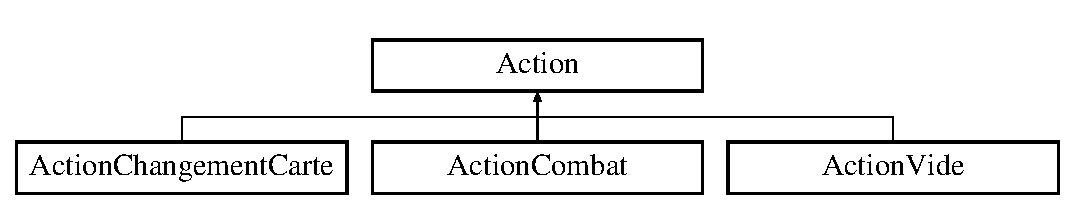
\includegraphics[height=2.000000cm]{classAction}
\end{center}
\end{figure}
\subsection*{Public Member Functions}
\begin{DoxyCompactItemize}
\item 
virtual void \hyperlink{classAction_a47d25fc7d6ef58692a7a4c5bc7e7fbd0}{lancer\-Action} ()=0
\begin{DoxyCompactList}\small\item\em Lancement de l'action. \end{DoxyCompactList}\item 
\hyperlink{classAction_ae7e1142cb3535c940dbc86f9a3b2da52}{Action} (string txt\-Int)
\begin{DoxyCompactList}\small\item\em Constructeur. \end{DoxyCompactList}\item 
string \hyperlink{classAction_a4d7ef820e27b3e23ae3e145e4ed3cb93}{get\-Texte\-Interaction} ()
\begin{DoxyCompactList}\small\item\em Getter texte\-Interaction. \end{DoxyCompactList}\item 
void \hyperlink{classAction_a2524956139b3e1bbd780270a2208356f}{set\-Texte\-Interaction} (string texte)
\begin{DoxyCompactList}\small\item\em Setter texte\-Interaction. \end{DoxyCompactList}\item 
\hypertarget{classAction_a2a71b81a01d34c124e9e13368be67d38}{void \hyperlink{classAction_a2a71b81a01d34c124e9e13368be67d38}{toggle\-Active} ()}\label{classAction_a2a71b81a01d34c124e9e13368be67d38}

\begin{DoxyCompactList}\small\item\em Passe la variable active de V\-R\-A\-I a F\-A\-U\-X et vise verca. \end{DoxyCompactList}\item 
bool \hyperlink{classAction_ab4fe74ad00f9192b4ab9959638d31a5e}{is\-Active} ()
\begin{DoxyCompactList}\small\item\em dit si l'action est active \end{DoxyCompactList}\end{DoxyCompactItemize}


\subsection{Detailed Description}
gestion actions 

Cette classe gère les actions enclenchées par l'accès à une case particulière 

\subsection{Constructor \& Destructor Documentation}
\hypertarget{classAction_ae7e1142cb3535c940dbc86f9a3b2da52}{\index{Action@{Action}!Action@{Action}}
\index{Action@{Action}!Action@{Action}}
\subsubsection[{Action}]{\setlength{\rightskip}{0pt plus 5cm}Action\-::\-Action (
\begin{DoxyParamCaption}
\item[{string}]{txt\-Int}
\end{DoxyParamCaption}
)}}\label{classAction_ae7e1142cb3535c940dbc86f9a3b2da52}


Constructeur. 


\begin{DoxyParams}{Parameters}
{\em txt\-Int} & le texte d'interaction Constructeur de la classe \hyperlink{classAction}{Action} \\
\hline
\end{DoxyParams}


\subsection{Member Function Documentation}
\hypertarget{classAction_a4d7ef820e27b3e23ae3e145e4ed3cb93}{\index{Action@{Action}!get\-Texte\-Interaction@{get\-Texte\-Interaction}}
\index{get\-Texte\-Interaction@{get\-Texte\-Interaction}!Action@{Action}}
\subsubsection[{get\-Texte\-Interaction}]{\setlength{\rightskip}{0pt plus 5cm}string Action\-::get\-Texte\-Interaction (
\begin{DoxyParamCaption}
{}
\end{DoxyParamCaption}
)}}\label{classAction_a4d7ef820e27b3e23ae3e145e4ed3cb93}


Getter texte\-Interaction. 

\begin{DoxyReturn}{Returns}
Le texte correspondant à l'action 
\end{DoxyReturn}
\hypertarget{classAction_ab4fe74ad00f9192b4ab9959638d31a5e}{\index{Action@{Action}!is\-Active@{is\-Active}}
\index{is\-Active@{is\-Active}!Action@{Action}}
\subsubsection[{is\-Active}]{\setlength{\rightskip}{0pt plus 5cm}bool Action\-::is\-Active (
\begin{DoxyParamCaption}
{}
\end{DoxyParamCaption}
)}}\label{classAction_ab4fe74ad00f9192b4ab9959638d31a5e}


dit si l'action est active 

\begin{DoxyReturn}{Returns}
L'état de l'action 
\end{DoxyReturn}
\hypertarget{classAction_a47d25fc7d6ef58692a7a4c5bc7e7fbd0}{\index{Action@{Action}!lancer\-Action@{lancer\-Action}}
\index{lancer\-Action@{lancer\-Action}!Action@{Action}}
\subsubsection[{lancer\-Action}]{\setlength{\rightskip}{0pt plus 5cm}void Action\-::lancer\-Action (
\begin{DoxyParamCaption}
{}
\end{DoxyParamCaption}
)\hspace{0.3cm}{\ttfamily [pure virtual]}}}\label{classAction_a47d25fc7d6ef58692a7a4c5bc7e7fbd0}


Lancement de l'action. 

Cette classe gère le lancement de l'action en fonction de la case où le joueur se trouve Cette méthode est abstraite, elle sera réimplémentée dans les classes héritant de \hyperlink{classAction}{Action} 

Implemented in \hyperlink{classActionChangementCarte_ac494368d1a8f41259761071bc27575e9}{Action\-Changement\-Carte}, \hyperlink{classActionCombat_a5f84011b92f33ea68b67e861d2c1a222}{Action\-Combat}, and \hyperlink{classActionVide_a6f318dcbb3cece06a8bd25a54842eeb0}{Action\-Vide}.

\hypertarget{classAction_a2524956139b3e1bbd780270a2208356f}{\index{Action@{Action}!set\-Texte\-Interaction@{set\-Texte\-Interaction}}
\index{set\-Texte\-Interaction@{set\-Texte\-Interaction}!Action@{Action}}
\subsubsection[{set\-Texte\-Interaction}]{\setlength{\rightskip}{0pt plus 5cm}string Action\-::set\-Texte\-Interaction (
\begin{DoxyParamCaption}
\item[{string}]{texte}
\end{DoxyParamCaption}
)}}\label{classAction_a2524956139b3e1bbd780270a2208356f}


Setter texte\-Interaction. 


\begin{DoxyParams}{Parameters}
{\em texte} & \-: Le texte correspondant à l'action \\
\hline
\end{DoxyParams}


The documentation for this class was generated from the following files\-:\begin{DoxyCompactItemize}
\item 
/home/damien/\-Bureau/projetcpp\-\_\-gm42/source/src/\hyperlink{Action_8hpp}{Action.\-hpp}\item 
/home/damien/\-Bureau/projetcpp\-\_\-gm42/source/src/Action.\-cpp\end{DoxyCompactItemize}

\hypertarget{classActionChangementCarte}{\section{Action\-Changement\-Carte Class Reference}
\label{classActionChangementCarte}\index{Action\-Changement\-Carte@{Action\-Changement\-Carte}}
}


gestion changement de carte  




{\ttfamily \#include $<$Action\-Changement\-Carte.\-hpp$>$}

Inheritance diagram for Action\-Changement\-Carte\-:\begin{figure}[H]
\begin{center}
\leavevmode
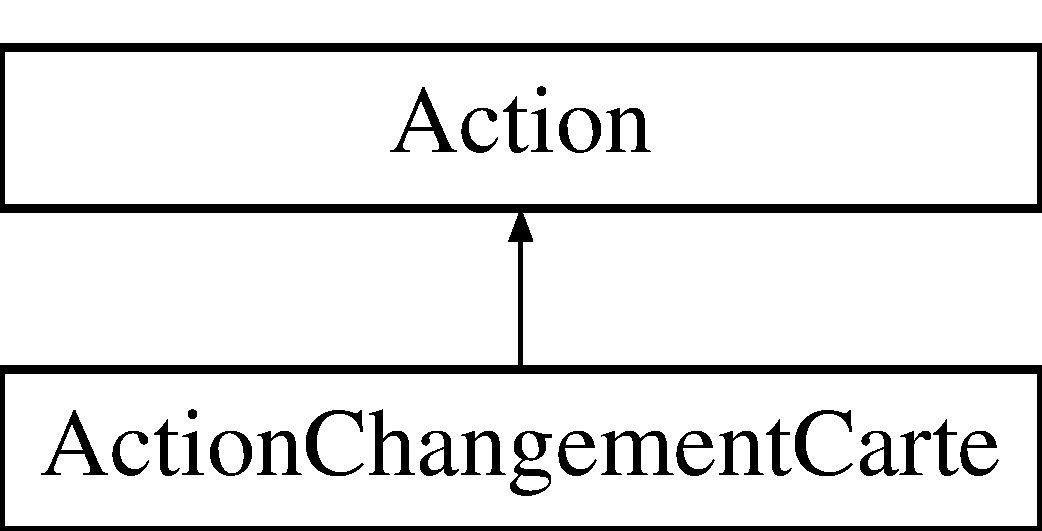
\includegraphics[height=2.000000cm]{classActionChangementCarte}
\end{center}
\end{figure}
\subsection*{Public Member Functions}
\begin{DoxyCompactItemize}
\item 
void \hyperlink{classActionChangementCarte_ac494368d1a8f41259761071bc27575e9}{lancer\-Action} ()
\begin{DoxyCompactList}\small\item\em Changement de carte. \end{DoxyCompactList}\item 
\hyperlink{classActionChangementCarte_ab576a1fe1f67249edfa612bde21c4a91}{Action\-Changement\-Carte} (\hyperlink{classCarte}{Carte} $\ast$carte\-Init, \hyperlink{classCarte}{Carte} $\ast$carte\-Dest, \hyperlink{classCoordonnees}{Coordonnees} coord\-Init, \hyperlink{classCoordonnees}{Coordonnees} coord\-Dest)
\begin{DoxyCompactList}\small\item\em Constructeur parametre. \end{DoxyCompactList}\end{DoxyCompactItemize}


\subsection{Detailed Description}
gestion changement de carte 

Cette classe gère le changement de \hyperlink{classCarte}{Carte} quand le joueur accède à une \hyperlink{classCellule}{Cellule} qui permet de changer de \hyperlink{classCarte}{Carte} 

\subsection{Constructor \& Destructor Documentation}
\hypertarget{classActionChangementCarte_ab576a1fe1f67249edfa612bde21c4a91}{\index{Action\-Changement\-Carte@{Action\-Changement\-Carte}!Action\-Changement\-Carte@{Action\-Changement\-Carte}}
\index{Action\-Changement\-Carte@{Action\-Changement\-Carte}!ActionChangementCarte@{Action\-Changement\-Carte}}
\subsubsection[{Action\-Changement\-Carte}]{\setlength{\rightskip}{0pt plus 5cm}Action\-Changement\-Carte\-::\-Action\-Changement\-Carte (
\begin{DoxyParamCaption}
\item[{{\bf Carte} $\ast$}]{carte\-Init, }
\item[{{\bf Carte} $\ast$}]{carte\-Dest, }
\item[{{\bf Coordonnees}}]{coord\-Init, }
\item[{{\bf Coordonnees}}]{coord\-Dest}
\end{DoxyParamCaption}
)}}\label{classActionChangementCarte_ab576a1fe1f67249edfa612bde21c4a91}


Constructeur parametre. 

Constructeur de la classe \hyperlink{classActionChangementCarte}{Action\-Changement\-Carte} 
\begin{DoxyParams}{Parameters}
{\em carte\-Init} & \-: \hyperlink{classCarte}{Carte} d'origine \\
\hline
{\em carte\-Dest} & \-: \hyperlink{classCarte}{Carte} de destination \\
\hline
{\em coord\-Init} & \-: \hyperlink{classCoordonnees}{Coordonnees} d'origine \\
\hline
{\em coord\-Dest} & \-: \hyperlink{classCoordonnees}{Coordonnees} de destination \\
\hline
\end{DoxyParams}


\subsection{Member Function Documentation}
\hypertarget{classActionChangementCarte_ac494368d1a8f41259761071bc27575e9}{\index{Action\-Changement\-Carte@{Action\-Changement\-Carte}!lancer\-Action@{lancer\-Action}}
\index{lancer\-Action@{lancer\-Action}!ActionChangementCarte@{Action\-Changement\-Carte}}
\subsubsection[{lancer\-Action}]{\setlength{\rightskip}{0pt plus 5cm}void Action\-Changement\-Carte\-::lancer\-Action (
\begin{DoxyParamCaption}
{}
\end{DoxyParamCaption}
)\hspace{0.3cm}{\ttfamily [virtual]}}}\label{classActionChangementCarte_ac494368d1a8f41259761071bc27575e9}


Changement de carte. 

Cette classe gère le changement de carte quand le joueur accède à une case qui permet de changer de carte 

Implements \hyperlink{classAction_a47d25fc7d6ef58692a7a4c5bc7e7fbd0}{Action}.



The documentation for this class was generated from the following files\-:\begin{DoxyCompactItemize}
\item 
/home/damien/\-Bureau/projetcpp\-\_\-gm42/source/src/\hyperlink{ActionChangementCarte_8hpp}{Action\-Changement\-Carte.\-hpp}\item 
/home/damien/\-Bureau/projetcpp\-\_\-gm42/source/src/Action\-Changement\-Carte.\-cpp\end{DoxyCompactItemize}

\hypertarget{classActionCombat}{\section{Action\-Combat Class Reference}
\label{classActionCombat}\index{Action\-Combat@{Action\-Combat}}
}


gestion lancement du combat  




{\ttfamily \#include $<$Action\-Combat.\-hpp$>$}

Inheritance diagram for Action\-Combat\-:\begin{figure}[H]
\begin{center}
\leavevmode
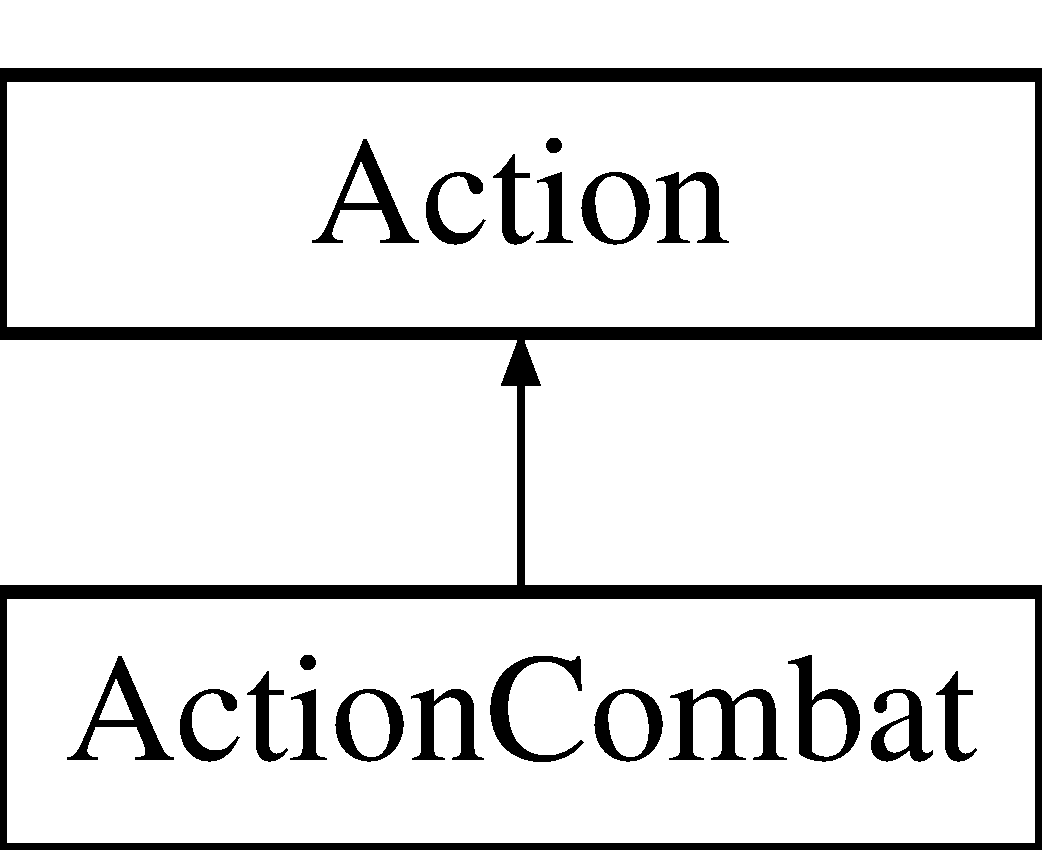
\includegraphics[height=2.000000cm]{classActionCombat}
\end{center}
\end{figure}
\subsection*{Public Member Functions}
\begin{DoxyCompactItemize}
\item 
\hyperlink{classActionCombat_a42da7041c76b15801f864c61e6e369d4}{Action\-Combat} (\hyperlink{classPersonnage}{Personnage} $\ast$adversairenv, string texte)
\begin{DoxyCompactList}\small\item\em Constructeur. \end{DoxyCompactList}\item 
void \hyperlink{classActionCombat_a5f84011b92f33ea68b67e861d2c1a222}{lancer\-Action} ()
\begin{DoxyCompactList}\small\item\em Lancement de l'action. \end{DoxyCompactList}\item 
\hyperlink{classPersonnage}{Personnage} $\ast$ \hyperlink{classActionCombat_ae9260ae03854f087cb60fd4a13dc395a}{get\-Adversaire} () const 
\begin{DoxyCompactList}\small\item\em getter \end{DoxyCompactList}\end{DoxyCompactItemize}


\subsection{Detailed Description}
gestion lancement du combat 

Cette classe lance un \hyperlink{classCombat}{Combat} lorsque le Joueur se trouve sur une case où il est menacé 

\subsection{Constructor \& Destructor Documentation}
\hypertarget{classActionCombat_a42da7041c76b15801f864c61e6e369d4}{\index{Action\-Combat@{Action\-Combat}!Action\-Combat@{Action\-Combat}}
\index{Action\-Combat@{Action\-Combat}!ActionCombat@{Action\-Combat}}
\subsubsection[{Action\-Combat}]{\setlength{\rightskip}{0pt plus 5cm}Action\-Combat\-::\-Action\-Combat (
\begin{DoxyParamCaption}
\item[{{\bf Personnage} $\ast$}]{adversairenv, }
\item[{string}]{texte}
\end{DoxyParamCaption}
)}}\label{classActionCombat_a42da7041c76b15801f864c61e6e369d4}


Constructeur. 

Constructeur de la classe \hyperlink{classActionCombat}{Action\-Combat} 
\begin{DoxyParams}{Parameters}
{\em texte} & texte a afficher \\
\hline
{\em adversairenv} & adversaire a affronter \\
\hline
\end{DoxyParams}


\subsection{Member Function Documentation}
\hypertarget{classActionCombat_ae9260ae03854f087cb60fd4a13dc395a}{\index{Action\-Combat@{Action\-Combat}!get\-Adversaire@{get\-Adversaire}}
\index{get\-Adversaire@{get\-Adversaire}!ActionCombat@{Action\-Combat}}
\subsubsection[{get\-Adversaire}]{\setlength{\rightskip}{0pt plus 5cm}{\bf Personnage} $\ast$ Action\-Combat\-::get\-Adversaire (
\begin{DoxyParamCaption}
{}
\end{DoxyParamCaption}
) const}}\label{classActionCombat_ae9260ae03854f087cb60fd4a13dc395a}


getter 

\begin{DoxyReturn}{Returns}
adversaire 
\end{DoxyReturn}
\hypertarget{classActionCombat_a5f84011b92f33ea68b67e861d2c1a222}{\index{Action\-Combat@{Action\-Combat}!lancer\-Action@{lancer\-Action}}
\index{lancer\-Action@{lancer\-Action}!ActionCombat@{Action\-Combat}}
\subsubsection[{lancer\-Action}]{\setlength{\rightskip}{0pt plus 5cm}void Action\-Combat\-::lancer\-Action (
\begin{DoxyParamCaption}
{}
\end{DoxyParamCaption}
)\hspace{0.3cm}{\ttfamily [virtual]}}}\label{classActionCombat_a5f84011b92f33ea68b67e861d2c1a222}


Lancement de l'action. 

Cette classe gère le lancement du combat en fonction de la case où le joueur se trouve 

Implements \hyperlink{classAction_a47d25fc7d6ef58692a7a4c5bc7e7fbd0}{Action}.



The documentation for this class was generated from the following files\-:\begin{DoxyCompactItemize}
\item 
/home/damien/\-Bureau/projetcpp\-\_\-gm42/source/src/\hyperlink{ActionCombat_8hpp}{Action\-Combat.\-hpp}\item 
/home/damien/\-Bureau/projetcpp\-\_\-gm42/source/src/Action\-Combat.\-cpp\end{DoxyCompactItemize}

\hypertarget{classActionVide}{\section{Action\-Vide Class Reference}
\label{classActionVide}\index{Action\-Vide@{Action\-Vide}}
}


Lance une action vide.  




{\ttfamily \#include $<$Action\-Vide.\-hpp$>$}

Inheritance diagram for Action\-Vide\-:\begin{figure}[H]
\begin{center}
\leavevmode
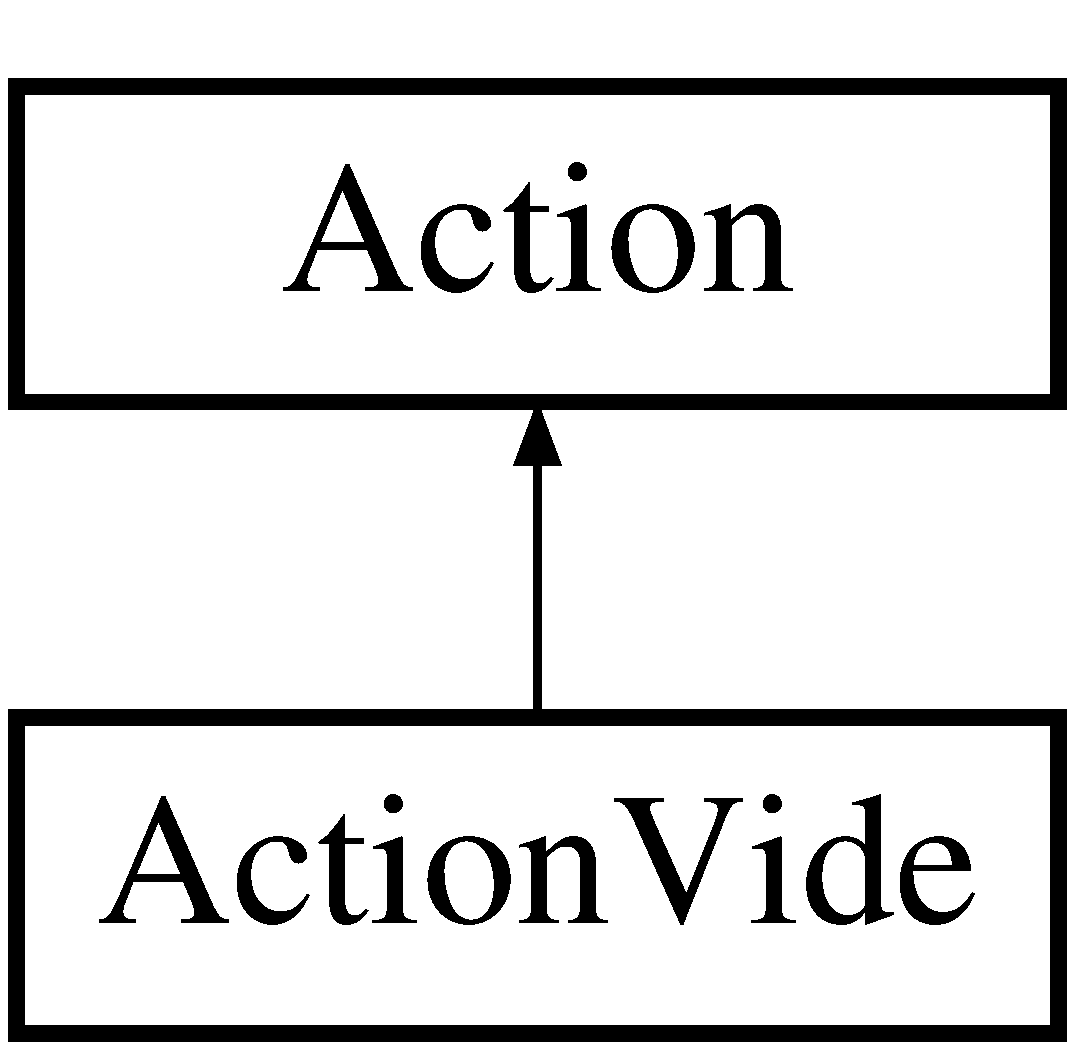
\includegraphics[height=2.000000cm]{classActionVide}
\end{center}
\end{figure}
\subsection*{Public Member Functions}
\begin{DoxyCompactItemize}
\item 
\hyperlink{classActionVide_ae395c7b2e008e7bba8eb32301a9c922b}{Action\-Vide} (string texte\-Init)
\item 
\hypertarget{classActionVide_a6f318dcbb3cece06a8bd25a54842eeb0}{void \hyperlink{classActionVide_a6f318dcbb3cece06a8bd25a54842eeb0}{lancer\-Action} ()}\label{classActionVide_a6f318dcbb3cece06a8bd25a54842eeb0}

\begin{DoxyCompactList}\small\item\em lancer autre action \end{DoxyCompactList}\end{DoxyCompactItemize}


\subsection{Detailed Description}
Lance une action vide. 

\subsection{Constructor \& Destructor Documentation}
\hypertarget{classActionVide_ae395c7b2e008e7bba8eb32301a9c922b}{\index{Action\-Vide@{Action\-Vide}!Action\-Vide@{Action\-Vide}}
\index{Action\-Vide@{Action\-Vide}!ActionVide@{Action\-Vide}}
\subsubsection[{Action\-Vide}]{\setlength{\rightskip}{0pt plus 5cm}Action\-Vide\-::\-Action\-Vide (
\begin{DoxyParamCaption}
\item[{string}]{texte\-Init}
\end{DoxyParamCaption}
)}}\label{classActionVide_ae395c7b2e008e7bba8eb32301a9c922b}
\textbackslash{} brief Constructeur 

The documentation for this class was generated from the following files\-:\begin{DoxyCompactItemize}
\item 
/home/damien/\-Bureau/projetcpp\-\_\-gm42/source/src/\hyperlink{ActionVide_8hpp}{Action\-Vide.\-hpp}\item 
/home/damien/\-Bureau/projetcpp\-\_\-gm42/source/src/Action\-Vide.\-cpp\end{DoxyCompactItemize}

\hypertarget{classArme}{\section{Arme Class Reference}
\label{classArme}\index{Arme@{Arme}}
}


gestion de l'arme  




{\ttfamily \#include $<$Arme.\-hpp$>$}

Inheritance diagram for Arme\-:\begin{figure}[H]
\begin{center}
\leavevmode
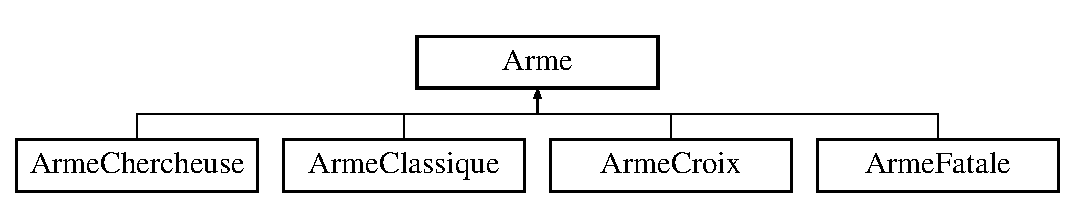
\includegraphics[height=2.000000cm]{classArme}
\end{center}
\end{figure}
\subsection*{Public Member Functions}
\begin{DoxyCompactItemize}
\item 
string \hyperlink{classArme_a46baac89e7062c4f111c1ee8b26e59df}{get\-Nom\-Arme} () const 
\begin{DoxyCompactList}\small\item\em getter de nom\-Arme \end{DoxyCompactList}\item 
void \hyperlink{classArme_a0aaf1c316ba1aa46768d73de58e059e2}{set\-Nom\-Arme} (const string nv\-Nom\-Arme)
\begin{DoxyCompactList}\small\item\em setter de nom\-Arme \end{DoxyCompactList}\item 
virtual void \hyperlink{classArme_a2092f960c2fb796bea3d9887775fa90e}{tirer} (const \hyperlink{classCoordonnees}{Coordonnees} coordonnees, \hyperlink{classGrille}{Grille} $\ast$grille)=0
\begin{DoxyCompactList}\small\item\em Attaque. \end{DoxyCompactList}\item 
\hyperlink{classArme_a31f873e62d4cc6f9c055ead94147ee77}{Arme} (string nom)
\begin{DoxyCompactList}\small\item\em Constructeur parametre de la classe \hyperlink{classArme}{Arme}. \end{DoxyCompactList}\end{DoxyCompactItemize}


\subsection{Detailed Description}
gestion de l'arme 

Cette classe gère les informations concernant l'arme du joueur 

\subsection{Constructor \& Destructor Documentation}
\hypertarget{classArme_a31f873e62d4cc6f9c055ead94147ee77}{\index{Arme@{Arme}!Arme@{Arme}}
\index{Arme@{Arme}!Arme@{Arme}}
\subsubsection[{Arme}]{\setlength{\rightskip}{0pt plus 5cm}Arme\-::\-Arme (
\begin{DoxyParamCaption}
\item[{string}]{nom}
\end{DoxyParamCaption}
)}}\label{classArme_a31f873e62d4cc6f9c055ead94147ee77}


Constructeur parametre de la classe \hyperlink{classArme}{Arme}. 


\begin{DoxyParams}{Parameters}
{\em nom} & \-: nom de l'arme \\
\hline
\end{DoxyParams}


\subsection{Member Function Documentation}
\hypertarget{classArme_a46baac89e7062c4f111c1ee8b26e59df}{\index{Arme@{Arme}!get\-Nom\-Arme@{get\-Nom\-Arme}}
\index{get\-Nom\-Arme@{get\-Nom\-Arme}!Arme@{Arme}}
\subsubsection[{get\-Nom\-Arme}]{\setlength{\rightskip}{0pt plus 5cm}string Arme\-::get\-Nom\-Arme (
\begin{DoxyParamCaption}
{}
\end{DoxyParamCaption}
) const}}\label{classArme_a46baac89e7062c4f111c1ee8b26e59df}


getter de nom\-Arme 

retourne le nom de l'\hyperlink{classArme}{Arme} \begin{DoxyReturn}{Returns}
string nom de l'arme 
\end{DoxyReturn}
\hypertarget{classArme_a0aaf1c316ba1aa46768d73de58e059e2}{\index{Arme@{Arme}!set\-Nom\-Arme@{set\-Nom\-Arme}}
\index{set\-Nom\-Arme@{set\-Nom\-Arme}!Arme@{Arme}}
\subsubsection[{set\-Nom\-Arme}]{\setlength{\rightskip}{0pt plus 5cm}void Arme\-::set\-Nom\-Arme (
\begin{DoxyParamCaption}
\item[{const string}]{nv\-Nom\-Arme}
\end{DoxyParamCaption}
)}}\label{classArme_a0aaf1c316ba1aa46768d73de58e059e2}


setter de nom\-Arme 

modifie le nom de l'\hyperlink{classArme}{Arme} 
\begin{DoxyParams}{Parameters}
{\em nv\-Nom\-Arme} & nom de l'\hyperlink{classArme}{Arme} \\
\hline
\end{DoxyParams}
\hypertarget{classArme_a2092f960c2fb796bea3d9887775fa90e}{\index{Arme@{Arme}!tirer@{tirer}}
\index{tirer@{tirer}!Arme@{Arme}}
\subsubsection[{tirer}]{\setlength{\rightskip}{0pt plus 5cm}void Arme\-::tirer (
\begin{DoxyParamCaption}
\item[{const {\bf Coordonnees}}]{coordonnees, }
\item[{{\bf Grille} $\ast$}]{grille}
\end{DoxyParamCaption}
)\hspace{0.3cm}{\ttfamily [pure virtual]}}}\label{classArme_a2092f960c2fb796bea3d9887775fa90e}


Attaque. 

tire sur une case et inflige des dégâts en fonction de l'arme utilisée 
\begin{DoxyParams}{Parameters}
{\em coordonnees} & \-: coordonnées de la case que le joueur souhaite viser \\
\hline
{\em $\ast$grille} & \-: pointeur sur la grille sur lequel le joueur tire \\
\hline
\end{DoxyParams}


Implemented in \hyperlink{classArmeChercheuse_ad3584a57b7b4fcee261b87fdd3c33806}{Arme\-Chercheuse}, \hyperlink{classArmeClassique_a0260158e5047726e694f376948dcaeca}{Arme\-Classique}, \hyperlink{classArmeCroix_a66a52523c2e6acf8f6c73fea8eb1cbcf}{Arme\-Croix}, and \hyperlink{classArmeFatale_a2e0c981f498b14ca79312d0a3ec34c70}{Arme\-Fatale}.



The documentation for this class was generated from the following files\-:\begin{DoxyCompactItemize}
\item 
/home/damien/\-Bureau/projetcpp\-\_\-gm42/source/src/\hyperlink{Arme_8hpp}{Arme.\-hpp}\item 
/home/damien/\-Bureau/projetcpp\-\_\-gm42/source/src/Arme.\-cpp\end{DoxyCompactItemize}

\hypertarget{classArmeChercheuse}{\section{Arme\-Chercheuse Class Reference}
\label{classArmeChercheuse}\index{Arme\-Chercheuse@{Arme\-Chercheuse}}
}


gestion de l'\hyperlink{classArme}{Arme} Chercheuse  




{\ttfamily \#include $<$Arme\-Chercheuse.\-hpp$>$}

Inheritance diagram for Arme\-Chercheuse\-:\begin{figure}[H]
\begin{center}
\leavevmode
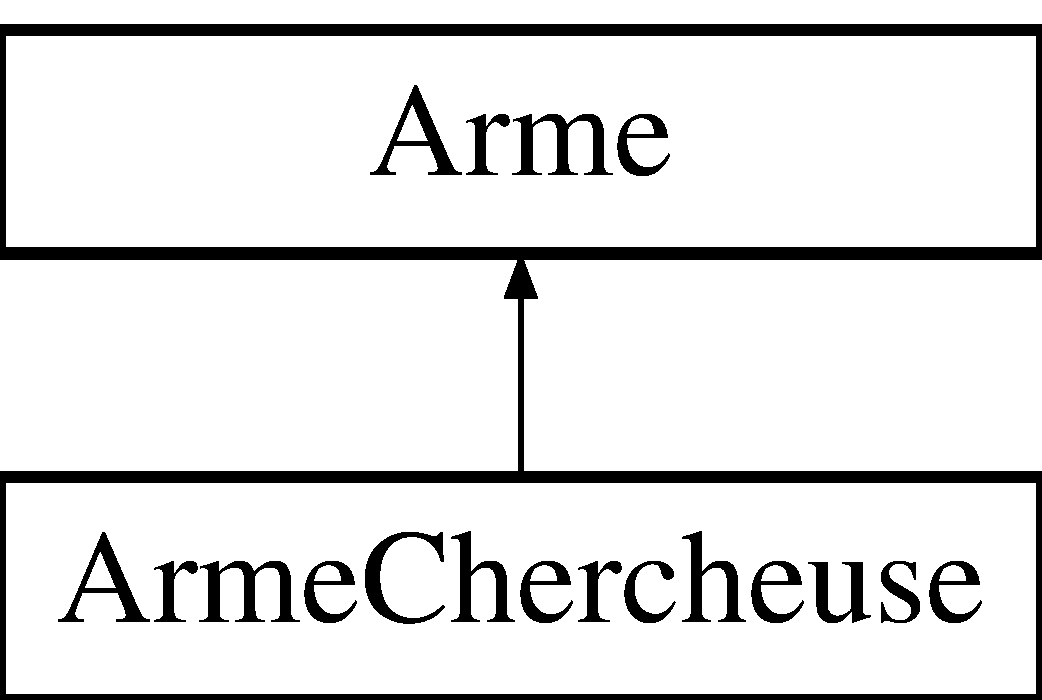
\includegraphics[height=2.000000cm]{classArmeChercheuse}
\end{center}
\end{figure}
\subsection*{Public Member Functions}
\begin{DoxyCompactItemize}
\item 
\hyperlink{classArmeChercheuse_acbcf8babee6bff7492933e739dfeeae0}{Arme\-Chercheuse} ()
\begin{DoxyCompactList}\small\item\em Construit une \hyperlink{classArme}{Arme} qui tire sur une case bateau de maniere aleatoire. \end{DoxyCompactList}\item 
void \hyperlink{classArmeChercheuse_ad3584a57b7b4fcee261b87fdd3c33806}{tirer} (\hyperlink{classCoordonnees}{Coordonnees} coordonnees, \hyperlink{classGrille}{Grille} $\ast$grille)
\begin{DoxyCompactList}\small\item\em Attaque Chercheuse. \end{DoxyCompactList}\end{DoxyCompactItemize}


\subsection{Detailed Description}
gestion de l'\hyperlink{classArme}{Arme} Chercheuse 

Cette classe gere les informations concernant l'arme du joueur 

\subsection{Constructor \& Destructor Documentation}
\hypertarget{classArmeChercheuse_acbcf8babee6bff7492933e739dfeeae0}{\index{Arme\-Chercheuse@{Arme\-Chercheuse}!Arme\-Chercheuse@{Arme\-Chercheuse}}
\index{Arme\-Chercheuse@{Arme\-Chercheuse}!ArmeChercheuse@{Arme\-Chercheuse}}
\subsubsection[{Arme\-Chercheuse}]{\setlength{\rightskip}{0pt plus 5cm}Arme\-Chercheuse\-::\-Arme\-Chercheuse (
\begin{DoxyParamCaption}
{}
\end{DoxyParamCaption}
)}}\label{classArmeChercheuse_acbcf8babee6bff7492933e739dfeeae0}


Construit une \hyperlink{classArme}{Arme} qui tire sur une case bateau de maniere aleatoire. 

\hyperlink{classArme}{Arme} tirant sur une case et inflige des degats sur ladite case 

\subsection{Member Function Documentation}
\hypertarget{classArmeChercheuse_ad3584a57b7b4fcee261b87fdd3c33806}{\index{Arme\-Chercheuse@{Arme\-Chercheuse}!tirer@{tirer}}
\index{tirer@{tirer}!ArmeChercheuse@{Arme\-Chercheuse}}
\subsubsection[{tirer}]{\setlength{\rightskip}{0pt plus 5cm}void Arme\-Chercheuse\-::tirer (
\begin{DoxyParamCaption}
\item[{{\bf Coordonnees}}]{coordonnees, }
\item[{{\bf Grille} $\ast$}]{grille}
\end{DoxyParamCaption}
)\hspace{0.3cm}{\ttfamily [virtual]}}}\label{classArmeChercheuse_ad3584a57b7b4fcee261b87fdd3c33806}


Attaque Chercheuse. 

Tire sur une case et inflige des degats sur ladite case 
\begin{DoxyParams}{Parameters}
{\em grille} & \-: pointeur sur la grille sur lequel le joueur tire \\
\hline
{\em coordonnees} & \hyperlink{classCoordonnees}{Coordonnees} visees \\
\hline
\end{DoxyParams}


Implements \hyperlink{classArme_a2092f960c2fb796bea3d9887775fa90e}{Arme}.



The documentation for this class was generated from the following files\-:\begin{DoxyCompactItemize}
\item 
/home/damien/\-Bureau/projetcpp\-\_\-gm42/source/src/\hyperlink{ArmeChercheuse_8hpp}{Arme\-Chercheuse.\-hpp}\item 
/home/damien/\-Bureau/projetcpp\-\_\-gm42/source/src/Arme\-Chercheuse.\-cpp\end{DoxyCompactItemize}

\hypertarget{classArmeClassique}{\section{Arme\-Classique Class Reference}
\label{classArmeClassique}\index{Arme\-Classique@{Arme\-Classique}}
}


gestion de l'\hyperlink{classArme}{Arme} Classique  




{\ttfamily \#include $<$Arme\-Classique.\-hpp$>$}

Inheritance diagram for Arme\-Classique\-:\begin{figure}[H]
\begin{center}
\leavevmode
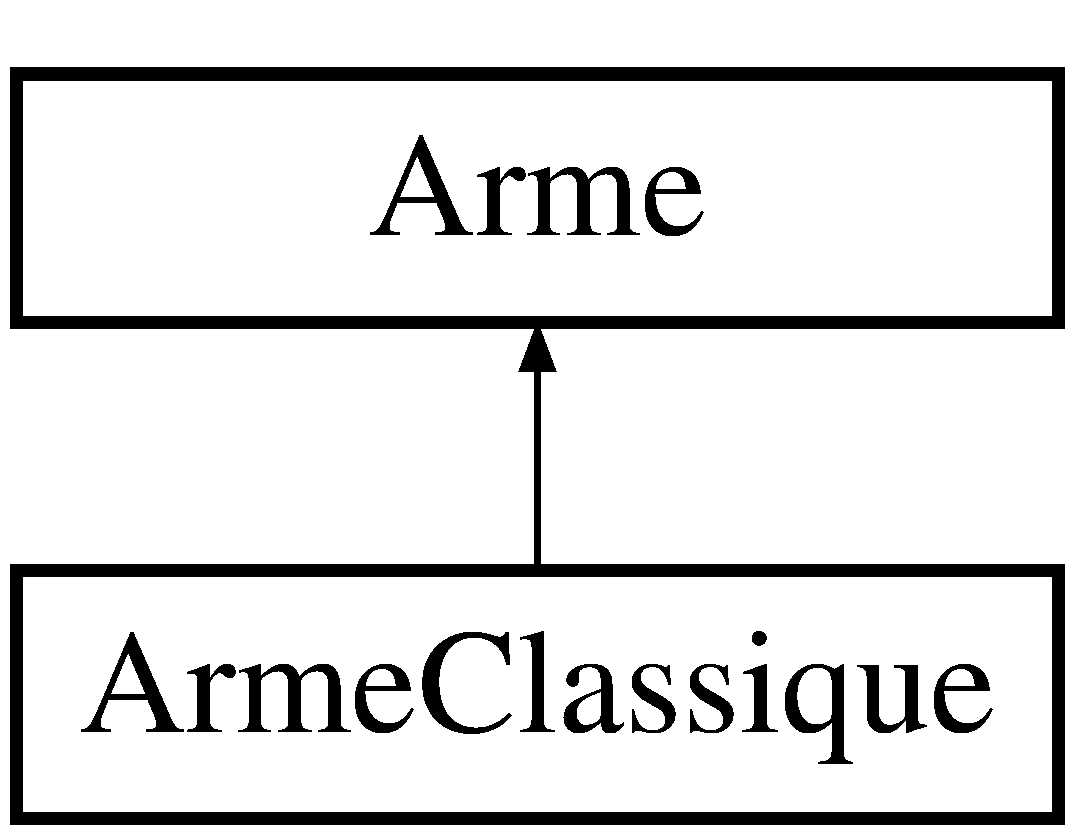
\includegraphics[height=2.000000cm]{classArmeClassique}
\end{center}
\end{figure}
\subsection*{Public Member Functions}
\begin{DoxyCompactItemize}
\item 
\hyperlink{classArmeClassique_a58581eaaecbd3dac969f8d0fb2ff9368}{Arme\-Classique} ()
\begin{DoxyCompactList}\small\item\em Construit une \hyperlink{classArme}{Arme} ne tirant que sur la \hyperlink{classCase}{Case} à Viser. \end{DoxyCompactList}\item 
void \hyperlink{classArmeClassique_a0260158e5047726e694f376948dcaeca}{tirer} (const \hyperlink{classCoordonnees}{Coordonnees} coordonnees, \hyperlink{classGrille}{Grille} $\ast$grille)
\begin{DoxyCompactList}\small\item\em Attaque classique. \end{DoxyCompactList}\end{DoxyCompactItemize}


\subsection{Detailed Description}
gestion de l'\hyperlink{classArme}{Arme} Classique 

Cette classe gère les informations concernant l'arme du joueur 

\subsection{Constructor \& Destructor Documentation}
\hypertarget{classArmeClassique_a58581eaaecbd3dac969f8d0fb2ff9368}{\index{Arme\-Classique@{Arme\-Classique}!Arme\-Classique@{Arme\-Classique}}
\index{Arme\-Classique@{Arme\-Classique}!ArmeClassique@{Arme\-Classique}}
\subsubsection[{Arme\-Classique}]{\setlength{\rightskip}{0pt plus 5cm}Arme\-Classique\-::\-Arme\-Classique (
\begin{DoxyParamCaption}
{}
\end{DoxyParamCaption}
)}}\label{classArmeClassique_a58581eaaecbd3dac969f8d0fb2ff9368}


Construit une \hyperlink{classArme}{Arme} ne tirant que sur la \hyperlink{classCase}{Case} à Viser. 

\hyperlink{classArme}{Arme} tirant sur une case et inflige des dégats sur ladite case 

\subsection{Member Function Documentation}
\hypertarget{classArmeClassique_a0260158e5047726e694f376948dcaeca}{\index{Arme\-Classique@{Arme\-Classique}!tirer@{tirer}}
\index{tirer@{tirer}!ArmeClassique@{Arme\-Classique}}
\subsubsection[{tirer}]{\setlength{\rightskip}{0pt plus 5cm}void Arme\-Classique\-::tirer (
\begin{DoxyParamCaption}
\item[{const {\bf Coordonnees}}]{coordonnees, }
\item[{{\bf Grille} $\ast$}]{grille}
\end{DoxyParamCaption}
)\hspace{0.3cm}{\ttfamily [virtual]}}}\label{classArmeClassique_a0260158e5047726e694f376948dcaeca}


Attaque classique. 

tire sur une case et inflige des dégats sur ladite case 
\begin{DoxyParams}{Parameters}
{\em coordonnees} & \-: coordonnées de la case que le joueur souhaite viser \\
\hline
{\em $\ast$grille} & \-: pointeur sur la grille sur lequel le joueur tire \\
\hline
\end{DoxyParams}


Implements \hyperlink{classArme_a2092f960c2fb796bea3d9887775fa90e}{Arme}.



The documentation for this class was generated from the following files\-:\begin{DoxyCompactItemize}
\item 
/home/damien/\-Bureau/projetcpp\-\_\-gm42/source/src/\hyperlink{ArmeClassique_8hpp}{Arme\-Classique.\-hpp}\item 
/home/damien/\-Bureau/projetcpp\-\_\-gm42/source/src/Arme\-Classique.\-cpp\end{DoxyCompactItemize}

\hypertarget{classArmeCroix}{\section{Arme\-Croix Class Reference}
\label{classArmeCroix}\index{Arme\-Croix@{Arme\-Croix}}
}


gestion de l'\hyperlink{classArme}{Arme} Croix  




{\ttfamily \#include $<$Arme\-Croix.\-hpp$>$}

Inheritance diagram for Arme\-Croix\-:\begin{figure}[H]
\begin{center}
\leavevmode
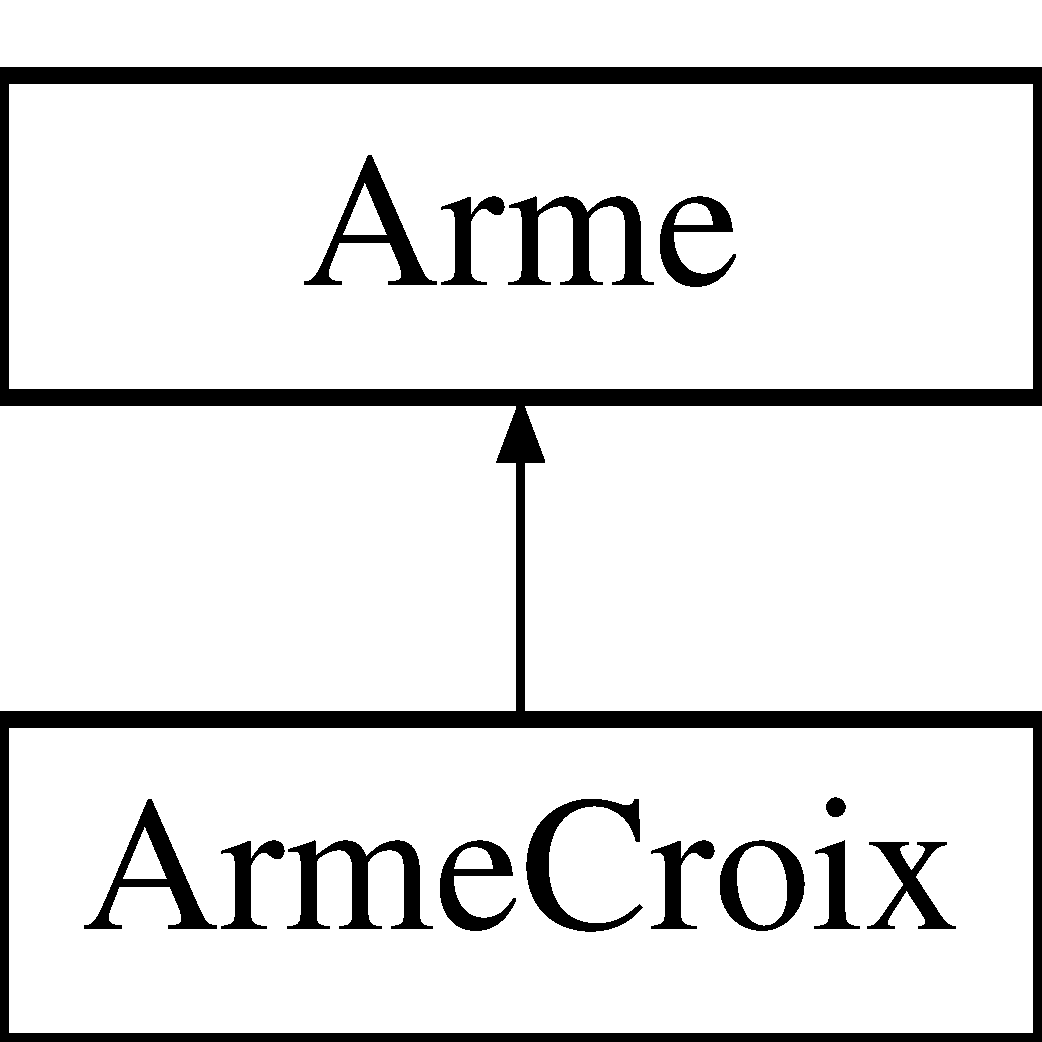
\includegraphics[height=2.000000cm]{classArmeCroix}
\end{center}
\end{figure}
\subsection*{Public Member Functions}
\begin{DoxyCompactItemize}
\item 
\hyperlink{classArmeCroix_ab0c53f82d21e934b1bac89f301f2fc7f}{Arme\-Croix} ()
\begin{DoxyCompactList}\small\item\em Construit une \hyperlink{classArme}{Arme} ne tirant en forme de croix sur la \hyperlink{classCase}{Case} a Viser. \end{DoxyCompactList}\item 
void \hyperlink{classArmeCroix_a66a52523c2e6acf8f6c73fea8eb1cbcf}{tirer} (const \hyperlink{classCoordonnees}{Coordonnees} coordonnees, \hyperlink{classGrille}{Grille} $\ast$grille)
\begin{DoxyCompactList}\small\item\em Attaque en croix. \end{DoxyCompactList}\end{DoxyCompactItemize}


\subsection{Detailed Description}
gestion de l'\hyperlink{classArme}{Arme} Croix 

Cette classe gere les informations concernant l'arme du joueur lorsqu'il utilise celle en Croix 

\subsection{Constructor \& Destructor Documentation}
\hypertarget{classArmeCroix_ab0c53f82d21e934b1bac89f301f2fc7f}{\index{Arme\-Croix@{Arme\-Croix}!Arme\-Croix@{Arme\-Croix}}
\index{Arme\-Croix@{Arme\-Croix}!ArmeCroix@{Arme\-Croix}}
\subsubsection[{Arme\-Croix}]{\setlength{\rightskip}{0pt plus 5cm}Arme\-Croix\-::\-Arme\-Croix (
\begin{DoxyParamCaption}
{}
\end{DoxyParamCaption}
)}}\label{classArmeCroix_ab0c53f82d21e934b1bac89f301f2fc7f}


Construit une \hyperlink{classArme}{Arme} ne tirant en forme de croix sur la \hyperlink{classCase}{Case} a Viser. 

\hyperlink{classArme}{Arme} tirant sur une case et inflige des degats sur ladite case et celles adjacentes 

\subsection{Member Function Documentation}
\hypertarget{classArmeCroix_a66a52523c2e6acf8f6c73fea8eb1cbcf}{\index{Arme\-Croix@{Arme\-Croix}!tirer@{tirer}}
\index{tirer@{tirer}!ArmeCroix@{Arme\-Croix}}
\subsubsection[{tirer}]{\setlength{\rightskip}{0pt plus 5cm}void Arme\-Croix\-::tirer (
\begin{DoxyParamCaption}
\item[{const {\bf Coordonnees}}]{coordonnees, }
\item[{{\bf Grille} $\ast$}]{grille}
\end{DoxyParamCaption}
)\hspace{0.3cm}{\ttfamily [virtual]}}}\label{classArmeCroix_a66a52523c2e6acf8f6c73fea8eb1cbcf}


Attaque en croix. 

tire sur une case et inflige des degats sur ladite case et celles adjacentes 
\begin{DoxyParams}{Parameters}
{\em coordonnees} & \-: coordonnees de la case que le joueur souhaite viser \\
\hline
{\em $\ast$grille} & \-: pointeur sur la grille sur lequel le joueur tire \\
\hline
\end{DoxyParams}


Implements \hyperlink{classArme_a2092f960c2fb796bea3d9887775fa90e}{Arme}.



The documentation for this class was generated from the following files\-:\begin{DoxyCompactItemize}
\item 
/home/damien/\-Bureau/projetcpp\-\_\-gm42/source/src/\hyperlink{ArmeCroix_8hpp}{Arme\-Croix.\-hpp}\item 
/home/damien/\-Bureau/projetcpp\-\_\-gm42/source/src/Arme\-Croix.\-cpp\end{DoxyCompactItemize}

\hypertarget{classArmeFatale}{\section{Arme\-Fatale Class Reference}
\label{classArmeFatale}\index{Arme\-Fatale@{Arme\-Fatale}}
}


gestion de l'\hyperlink{classArme}{Arme} Fatale  




{\ttfamily \#include $<$Arme\-Fatale.\-hpp$>$}

Inheritance diagram for Arme\-Fatale\-:\begin{figure}[H]
\begin{center}
\leavevmode
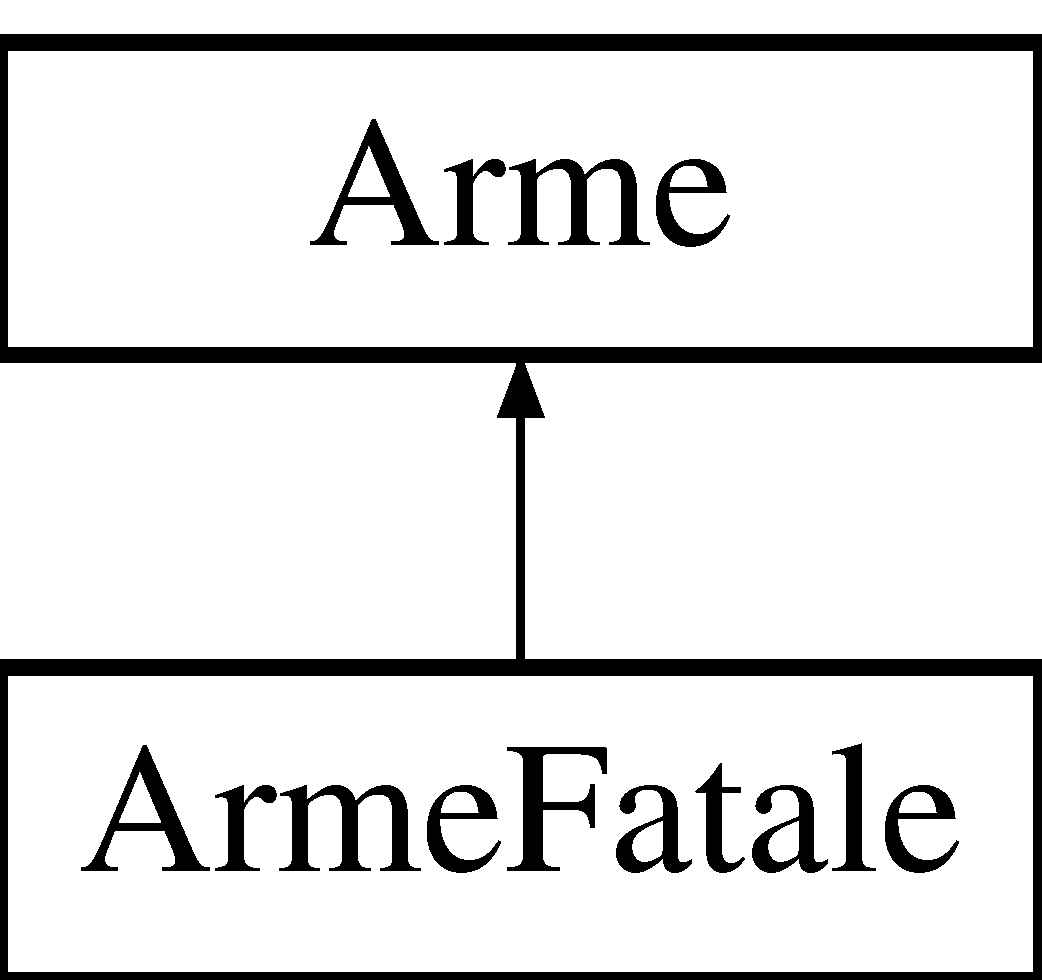
\includegraphics[height=2.000000cm]{classArmeFatale}
\end{center}
\end{figure}
\subsection*{Public Member Functions}
\begin{DoxyCompactItemize}
\item 
\hyperlink{classArmeFatale_a6e6abe097d84c4d7266cc675d0ead182}{Arme\-Fatale} ()
\begin{DoxyCompactList}\small\item\em Construit une \hyperlink{classArme}{Arme} Fatale. \end{DoxyCompactList}\item 
void \hyperlink{classArmeFatale_a2e0c981f498b14ca79312d0a3ec34c70}{tirer} (const \hyperlink{classCoordonnees}{Coordonnees} coordonnees, \hyperlink{classGrille}{Grille} $\ast$grille)
\begin{DoxyCompactList}\small\item\em Attaque classique. \end{DoxyCompactList}\end{DoxyCompactItemize}


\subsection{Detailed Description}
gestion de l'\hyperlink{classArme}{Arme} Fatale 

Cette classe gère les informations concernant l'arme du joueur 

\subsection{Constructor \& Destructor Documentation}
\hypertarget{classArmeFatale_a6e6abe097d84c4d7266cc675d0ead182}{\index{Arme\-Fatale@{Arme\-Fatale}!Arme\-Fatale@{Arme\-Fatale}}
\index{Arme\-Fatale@{Arme\-Fatale}!ArmeFatale@{Arme\-Fatale}}
\subsubsection[{Arme\-Fatale}]{\setlength{\rightskip}{0pt plus 5cm}Arme\-Fatale\-::\-Arme\-Fatale (
\begin{DoxyParamCaption}
{}
\end{DoxyParamCaption}
)}}\label{classArmeFatale_a6e6abe097d84c4d7266cc675d0ead182}


Construit une \hyperlink{classArme}{Arme} Fatale. 

\hyperlink{classArme}{Arme} qui détruit tout un bateau si elle en touche un sinon tire normalement 

\subsection{Member Function Documentation}
\hypertarget{classArmeFatale_a2e0c981f498b14ca79312d0a3ec34c70}{\index{Arme\-Fatale@{Arme\-Fatale}!tirer@{tirer}}
\index{tirer@{tirer}!ArmeFatale@{Arme\-Fatale}}
\subsubsection[{tirer}]{\setlength{\rightskip}{0pt plus 5cm}void Arme\-Fatale\-::tirer (
\begin{DoxyParamCaption}
\item[{const {\bf Coordonnees}}]{coordonnees, }
\item[{{\bf Grille} $\ast$}]{grille}
\end{DoxyParamCaption}
)\hspace{0.3cm}{\ttfamily [virtual]}}}\label{classArmeFatale_a2e0c981f498b14ca79312d0a3ec34c70}


Attaque classique. 

\hyperlink{classArme}{Arme} qui détruit tout un bateau si elle en touche un sinon tire normalement 
\begin{DoxyParams}{Parameters}
{\em coordonnees} & \-: coordonnées de la case que le joueur souhaite viser \\
\hline
{\em $\ast$grille} & \-: pointeur sur la grille sur lequel le joueur tire \\
\hline
\end{DoxyParams}


Implements \hyperlink{classArme_a2092f960c2fb796bea3d9887775fa90e}{Arme}.



The documentation for this class was generated from the following files\-:\begin{DoxyCompactItemize}
\item 
/home/damien/\-Bureau/projetcpp\-\_\-gm42/source/src/\hyperlink{ArmeFatale_8hpp}{Arme\-Fatale.\-hpp}\item 
/home/damien/\-Bureau/projetcpp\-\_\-gm42/source/src/Arme\-Fatale.\-cpp\end{DoxyCompactItemize}

\hypertarget{classBadgeFinal}{\section{Badge\-Final Class Reference}
\label{classBadgeFinal}\index{Badge\-Final@{Badge\-Final}}
}


Gestion des badges finaux.  




{\ttfamily \#include $<$Badge\-Final.\-hpp$>$}

Inheritance diagram for Badge\-Final\-:\begin{figure}[H]
\begin{center}
\leavevmode
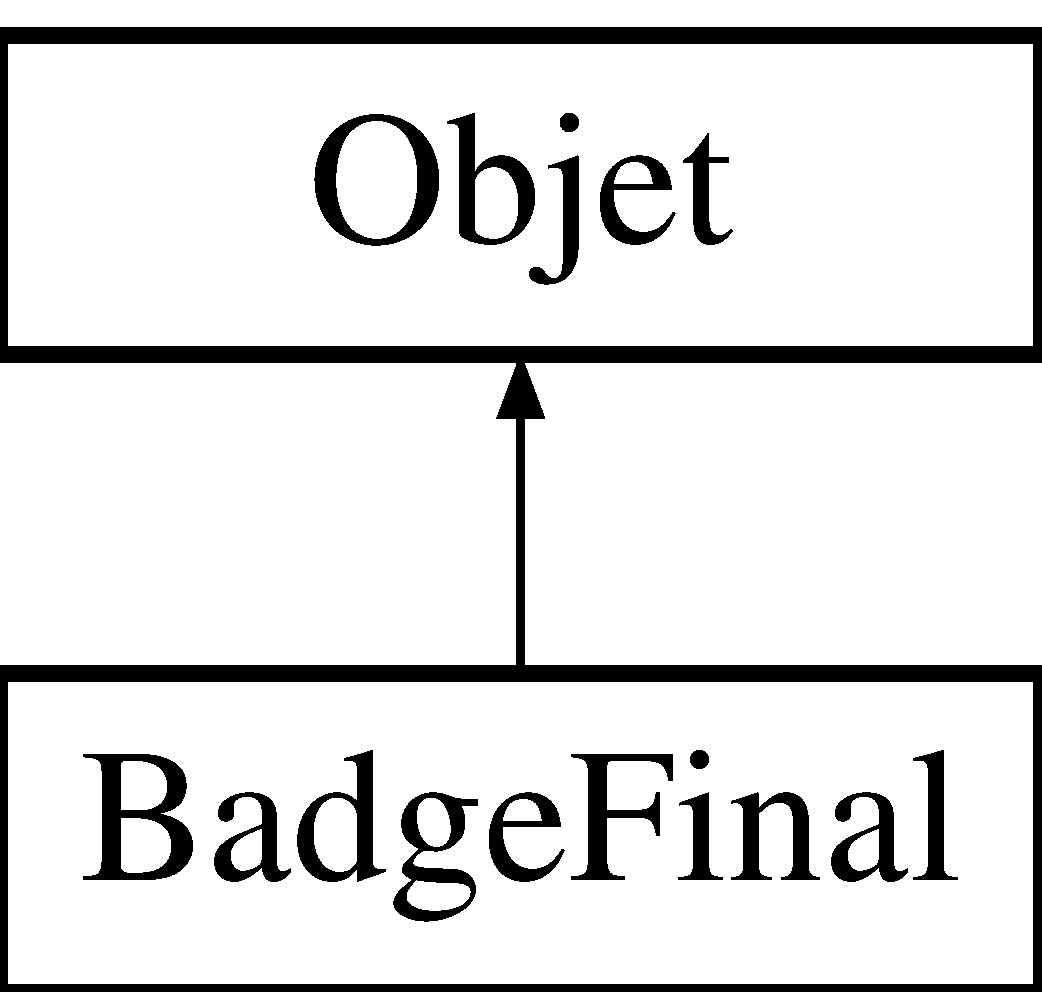
\includegraphics[height=2.000000cm]{classBadgeFinal}
\end{center}
\end{figure}
\subsection*{Public Member Functions}
\begin{DoxyCompactItemize}
\item 
\hypertarget{classBadgeFinal_a96c7204b62fea66c12d4dd3fe9bd0efb}{\hyperlink{classBadgeFinal_a96c7204b62fea66c12d4dd3fe9bd0efb}{Badge\-Final} ()}\label{classBadgeFinal_a96c7204b62fea66c12d4dd3fe9bd0efb}

\begin{DoxyCompactList}\small\item\em constructeur du badge final \end{DoxyCompactList}\item 
\hypertarget{classBadgeFinal_a257a6c9b681399ba8e5f7ae8ec065cc6}{virtual bool \hyperlink{classBadgeFinal_a257a6c9b681399ba8e5f7ae8ec065cc6}{met\-Fin\-Au\-Jeu} () const }\label{classBadgeFinal_a257a6c9b681399ba8e5f7ae8ec065cc6}

\begin{DoxyCompactList}\small\item\em Methode Virtuelle pure retournant si l'objet met fin au jeu. \end{DoxyCompactList}\end{DoxyCompactItemize}


\subsection{Detailed Description}
Gestion des badges finaux. 

Cette classe gère les informations concernant les badges finaux 

The documentation for this class was generated from the following files\-:\begin{DoxyCompactItemize}
\item 
/home/damien/\-Bureau/projetcpp\-\_\-gm42/source/src/\hyperlink{BadgeFinal_8hpp}{Badge\-Final.\-hpp}\item 
/home/damien/\-Bureau/projetcpp\-\_\-gm42/source/src/Badge\-Final.\-cpp\end{DoxyCompactItemize}

\hypertarget{classBatailleNavale}{\section{Bataille\-Navale Class Reference}
\label{classBatailleNavale}\index{Bataille\-Navale@{Bataille\-Navale}}
}


classe combat bataille navale  




{\ttfamily \#include $<$Bataille\-Navale.\-hpp$>$}

Inheritance diagram for Bataille\-Navale\-:\begin{figure}[H]
\begin{center}
\leavevmode
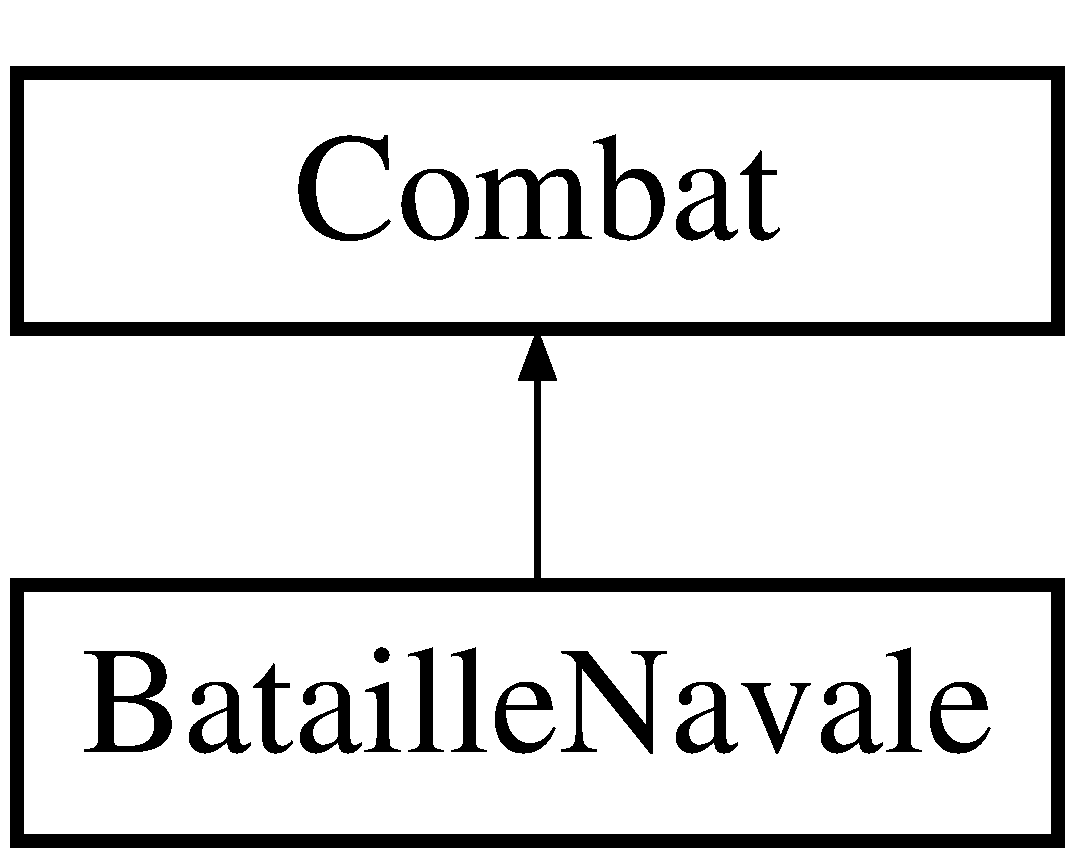
\includegraphics[height=2.000000cm]{classBatailleNavale}
\end{center}
\end{figure}
\subsection*{Public Member Functions}
\begin{DoxyCompactItemize}
\item 
\hyperlink{classBatailleNavale_a74cc728a7d2f09243e938cca13c16f59}{Bataille\-Navale} ()
\begin{DoxyCompactList}\small\item\em Constructeur. \end{DoxyCompactList}\item 
void \hyperlink{classBatailleNavale_a2dae6d08ff0e391f23e2775ff01de3d0}{jouer} (\hyperlink{classCoordonnees}{Coordonnees} coordonnees)
\begin{DoxyCompactList}\small\item\em Joueur vise case choisie. \end{DoxyCompactList}\item 
\hyperlink{classPersonnageBN}{Personnage\-B\-N} $\ast$ \hyperlink{classBatailleNavale_a06536e39a82ccaee6cc415a79d471427}{get\-Personnage1} () const 
\begin{DoxyCompactList}\small\item\em Getter du Joueur 1. \end{DoxyCompactList}\item 
\hyperlink{classPersonnageBN}{Personnage\-B\-N} $\ast$ \hyperlink{classBatailleNavale_a21fdc28f984238126557f7a5d5a005ba}{get\-Personnage2} () const 
\begin{DoxyCompactList}\small\item\em Getter du Joueur 2. \end{DoxyCompactList}\item 
\hyperlink{classGrille}{Grille} $\ast$ \hyperlink{classBatailleNavale_a8af0c5c56b59b7fbbf13e40f3bd1d703}{get\-Grille1} ()
\begin{DoxyCompactList}\small\item\em Getter de la grille 1. \end{DoxyCompactList}\item 
\hyperlink{classGrille}{Grille} $\ast$ \hyperlink{classBatailleNavale_a14d7cccff168cd71b0dedaa9f9b1cb68}{get\-Grille2} ()
\begin{DoxyCompactList}\small\item\em Getter de la grille 2. \end{DoxyCompactList}\item 
int \hyperlink{classBatailleNavale_a3ad348fe72fe0c727ffb59aea478a2f1}{get\-Indice\-Joueur\-Courant} () const 
\begin{DoxyCompactList}\small\item\em Getter de l indice du joueur courant. \end{DoxyCompactList}\item 
void \hyperlink{classBatailleNavale_a7afd1b0024f7e3df851880ce63289b21}{set\-Indice\-Joueur\-Courant} (const int nv\-Indice)
\begin{DoxyCompactList}\small\item\em Setter de l indice du joueur courant. \end{DoxyCompactList}\item 
vector$<$ \hyperlink{classPersonnageBN}{Personnage\-B\-N} $\ast$ $>$ \hyperlink{classBatailleNavale_a9fadbc201334aac3d7e181363483f12c}{get\-Joueurs} () const 
\begin{DoxyCompactList}\small\item\em Getter de la liste de Joueurs. \end{DoxyCompactList}\item 
vector$<$ \hyperlink{classGrille}{Grille} $\ast$ $>$ \hyperlink{classBatailleNavale_a2834333a3f934ea4d25f6f09139e740e}{get\-Grilles} ()
\begin{DoxyCompactList}\small\item\em Getter de l'ensemble des grilles. \end{DoxyCompactList}\item 
\hyperlink{classPersonnage}{Personnage} $\ast$ \hyperlink{classBatailleNavale_acff7cd9717a2ed3084b232d95ea9042a}{retourner\-Gagnant} (\hyperlink{classPersonnage}{Personnage} $\ast$joueur1, \hyperlink{classPersonnage}{Personnage} $\ast$joueur2)
\begin{DoxyCompactList}\small\item\em Retourner Gagnant. \end{DoxyCompactList}\item 
\hyperlink{classPersonnageBN}{Personnage\-B\-N} $\ast$ \hyperlink{classBatailleNavale_a6dd55fdc58c85d5fc7d2aceec872dcc0}{retourner\-Gagnant} ()
\begin{DoxyCompactList}\small\item\em Retourner Gagnant. \end{DoxyCompactList}\item 
void \hyperlink{classBatailleNavale_a503ea394595b67fb2101dc5a77c46e7c}{initialiser\-Joueur\-Courant} (\hyperlink{classPersonnageBN}{Personnage\-B\-N} $\ast$joueur1, \hyperlink{classPersonnageBN}{Personnage\-B\-N} $\ast$joueur2)
\begin{DoxyCompactList}\small\item\em initialise le joueur et les grilles \end{DoxyCompactList}\end{DoxyCompactItemize}


\subsection{Detailed Description}
classe combat bataille navale 

La classe gère la partie\-: l'initialise, crée les grilles, place les bateaux, permet aux joueurs de viser les cases, et modifie les grilles à chaque tour 

\subsection{Constructor \& Destructor Documentation}
\hypertarget{classBatailleNavale_a74cc728a7d2f09243e938cca13c16f59}{\index{Bataille\-Navale@{Bataille\-Navale}!Bataille\-Navale@{Bataille\-Navale}}
\index{Bataille\-Navale@{Bataille\-Navale}!BatailleNavale@{Bataille\-Navale}}
\subsubsection[{Bataille\-Navale}]{\setlength{\rightskip}{0pt plus 5cm}Bataille\-Navale\-::\-Bataille\-Navale (
\begin{DoxyParamCaption}
{}
\end{DoxyParamCaption}
)}}\label{classBatailleNavale_a74cc728a7d2f09243e938cca13c16f59}


Constructeur. 

Constructeur de la classe Bataille Navale Initialise les 2 joueurs, crée les 2 grilles de taille taille\-Grille à partir des joueurs puis va demander aux joueurs de placer leurs bateaux via la méthode placer\-Bateaux 

\subsection{Member Function Documentation}
\hypertarget{classBatailleNavale_a8af0c5c56b59b7fbbf13e40f3bd1d703}{\index{Bataille\-Navale@{Bataille\-Navale}!get\-Grille1@{get\-Grille1}}
\index{get\-Grille1@{get\-Grille1}!BatailleNavale@{Bataille\-Navale}}
\subsubsection[{get\-Grille1}]{\setlength{\rightskip}{0pt plus 5cm}{\bf Grille} Bataille\-Navale\-::get\-Grille1 (
\begin{DoxyParamCaption}
{}
\end{DoxyParamCaption}
)}}\label{classBatailleNavale_a8af0c5c56b59b7fbbf13e40f3bd1d703}


Getter de la grille 1. 

\begin{DoxyReturn}{Returns}
\hyperlink{classGrille}{Grille}\-: grille 1 
\end{DoxyReturn}
\hypertarget{classBatailleNavale_a14d7cccff168cd71b0dedaa9f9b1cb68}{\index{Bataille\-Navale@{Bataille\-Navale}!get\-Grille2@{get\-Grille2}}
\index{get\-Grille2@{get\-Grille2}!BatailleNavale@{Bataille\-Navale}}
\subsubsection[{get\-Grille2}]{\setlength{\rightskip}{0pt plus 5cm}{\bf Grille} Bataille\-Navale\-::get\-Grille2 (
\begin{DoxyParamCaption}
{}
\end{DoxyParamCaption}
)}}\label{classBatailleNavale_a14d7cccff168cd71b0dedaa9f9b1cb68}


Getter de la grille 2. 

\begin{DoxyReturn}{Returns}
\hyperlink{classGrille}{Grille}\-: grille 2 
\end{DoxyReturn}
\hypertarget{classBatailleNavale_a2834333a3f934ea4d25f6f09139e740e}{\index{Bataille\-Navale@{Bataille\-Navale}!get\-Grilles@{get\-Grilles}}
\index{get\-Grilles@{get\-Grilles}!BatailleNavale@{Bataille\-Navale}}
\subsubsection[{get\-Grilles}]{\setlength{\rightskip}{0pt plus 5cm}vector$<$ {\bf Grille} $>$ Bataille\-Navale\-::get\-Grilles (
\begin{DoxyParamCaption}
{}
\end{DoxyParamCaption}
)}}\label{classBatailleNavale_a2834333a3f934ea4d25f6f09139e740e}


Getter de l'ensemble des grilles. 

\begin{DoxyReturn}{Returns}
vector$<$\-Grille$>$\-: Ensemble des grilles 
\end{DoxyReturn}
\hypertarget{classBatailleNavale_a3ad348fe72fe0c727ffb59aea478a2f1}{\index{Bataille\-Navale@{Bataille\-Navale}!get\-Indice\-Joueur\-Courant@{get\-Indice\-Joueur\-Courant}}
\index{get\-Indice\-Joueur\-Courant@{get\-Indice\-Joueur\-Courant}!BatailleNavale@{Bataille\-Navale}}
\subsubsection[{get\-Indice\-Joueur\-Courant}]{\setlength{\rightskip}{0pt plus 5cm}int Bataille\-Navale\-::get\-Indice\-Joueur\-Courant (
\begin{DoxyParamCaption}
{}
\end{DoxyParamCaption}
) const}}\label{classBatailleNavale_a3ad348fe72fe0c727ffb59aea478a2f1}


Getter de l indice du joueur courant. 

\begin{DoxyReturn}{Returns}
int\-:indice du personnage courant 
\end{DoxyReturn}
\hypertarget{classBatailleNavale_a9fadbc201334aac3d7e181363483f12c}{\index{Bataille\-Navale@{Bataille\-Navale}!get\-Joueurs@{get\-Joueurs}}
\index{get\-Joueurs@{get\-Joueurs}!BatailleNavale@{Bataille\-Navale}}
\subsubsection[{get\-Joueurs}]{\setlength{\rightskip}{0pt plus 5cm}vector$<$ {\bf Personnage\-B\-N} $\ast$ $>$ Bataille\-Navale\-::get\-Joueurs (
\begin{DoxyParamCaption}
{}
\end{DoxyParamCaption}
) const}}\label{classBatailleNavale_a9fadbc201334aac3d7e181363483f12c}


Getter de la liste de Joueurs. 

\begin{DoxyReturn}{Returns}
vector$<$\-Personnage\-B\-N$\ast$$>$\-:vecteur des 2 joueurs s'affrontant à la Bataille Navale 
\end{DoxyReturn}
\hypertarget{classBatailleNavale_a06536e39a82ccaee6cc415a79d471427}{\index{Bataille\-Navale@{Bataille\-Navale}!get\-Personnage1@{get\-Personnage1}}
\index{get\-Personnage1@{get\-Personnage1}!BatailleNavale@{Bataille\-Navale}}
\subsubsection[{get\-Personnage1}]{\setlength{\rightskip}{0pt plus 5cm}{\bf Personnage\-B\-N} $\ast$ Bataille\-Navale\-::get\-Personnage1 (
\begin{DoxyParamCaption}
{}
\end{DoxyParamCaption}
) const}}\label{classBatailleNavale_a06536e39a82ccaee6cc415a79d471427}


Getter du Joueur 1. 

\begin{DoxyReturn}{Returns}
Personnage\-B\-N$\ast$\-: pointeur sur personnage 1 
\end{DoxyReturn}
\hypertarget{classBatailleNavale_a21fdc28f984238126557f7a5d5a005ba}{\index{Bataille\-Navale@{Bataille\-Navale}!get\-Personnage2@{get\-Personnage2}}
\index{get\-Personnage2@{get\-Personnage2}!BatailleNavale@{Bataille\-Navale}}
\subsubsection[{get\-Personnage2}]{\setlength{\rightskip}{0pt plus 5cm}{\bf Personnage\-B\-N} $\ast$ Bataille\-Navale\-::get\-Personnage2 (
\begin{DoxyParamCaption}
{}
\end{DoxyParamCaption}
) const}}\label{classBatailleNavale_a21fdc28f984238126557f7a5d5a005ba}


Getter du Joueur 2. 

\begin{DoxyReturn}{Returns}
Personnage\-B\-N$\ast$\-: pointeur sur personnage 2 
\end{DoxyReturn}
\hypertarget{classBatailleNavale_a503ea394595b67fb2101dc5a77c46e7c}{\index{Bataille\-Navale@{Bataille\-Navale}!initialiser\-Joueur\-Courant@{initialiser\-Joueur\-Courant}}
\index{initialiser\-Joueur\-Courant@{initialiser\-Joueur\-Courant}!BatailleNavale@{Bataille\-Navale}}
\subsubsection[{initialiser\-Joueur\-Courant}]{\setlength{\rightskip}{0pt plus 5cm}void Bataille\-Navale\-::initialiser\-Joueur\-Courant (
\begin{DoxyParamCaption}
\item[{{\bf Personnage\-B\-N} $\ast$}]{joueur1, }
\item[{{\bf Personnage\-B\-N} $\ast$}]{joueur2}
\end{DoxyParamCaption}
)}}\label{classBatailleNavale_a503ea394595b67fb2101dc5a77c46e7c}


initialise le joueur et les grilles 


\begin{DoxyParams}{Parameters}
{\em joueur1} & \-: représente le premier joueur du combat \\
\hline
{\em joueur2} & \-: représente le deuxième joueur du combat\\
\hline
\end{DoxyParams}
Méthode qui initialise les joueurs \hypertarget{classBatailleNavale_a2dae6d08ff0e391f23e2775ff01de3d0}{\index{Bataille\-Navale@{Bataille\-Navale}!jouer@{jouer}}
\index{jouer@{jouer}!BatailleNavale@{Bataille\-Navale}}
\subsubsection[{jouer}]{\setlength{\rightskip}{0pt plus 5cm}void Bataille\-Navale\-::jouer (
\begin{DoxyParamCaption}
\item[{{\bf Coordonnees}}]{coordonnees}
\end{DoxyParamCaption}
)}}\label{classBatailleNavale_a2dae6d08ff0e391f23e2775ff01de3d0}


Joueur vise case choisie. 

Le joueur courant vise la case à jouer et tire avec son arme (actualisation des grilles) puis changement de joueur courant 
\begin{DoxyParams}{Parameters}
{\em coordonnees} & coordonnées choisies par le joueur \\
\hline
\end{DoxyParams}
\hypertarget{classBatailleNavale_acff7cd9717a2ed3084b232d95ea9042a}{\index{Bataille\-Navale@{Bataille\-Navale}!retourner\-Gagnant@{retourner\-Gagnant}}
\index{retourner\-Gagnant@{retourner\-Gagnant}!BatailleNavale@{Bataille\-Navale}}
\subsubsection[{retourner\-Gagnant}]{\setlength{\rightskip}{0pt plus 5cm}{\bf Personnage} $\ast$ Bataille\-Navale\-::retourner\-Gagnant (
\begin{DoxyParamCaption}
\item[{{\bf Personnage} $\ast$}]{joueur1, }
\item[{{\bf Personnage} $\ast$}]{joueur2}
\end{DoxyParamCaption}
)\hspace{0.3cm}{\ttfamily [virtual]}}}\label{classBatailleNavale_acff7cd9717a2ed3084b232d95ea9042a}


Retourner Gagnant. 


\begin{DoxyParams}{Parameters}
{\em joueur1} & représente le premier joueur initial de notre combat \\
\hline
{\em joueur2} & représente le deuxième joueur initial de notre combat\\
\hline
\end{DoxyParams}
Méthode qui renvoie le gagnant du combat \begin{DoxyReturn}{Returns}
un personnage correspondant au gagnant et null si la partie n'est pas finie 
\end{DoxyReturn}


Implements \hyperlink{classCombat_a5b480832873d1bf4e8a91f1c7054e646}{Combat}.

\hypertarget{classBatailleNavale_a6dd55fdc58c85d5fc7d2aceec872dcc0}{\index{Bataille\-Navale@{Bataille\-Navale}!retourner\-Gagnant@{retourner\-Gagnant}}
\index{retourner\-Gagnant@{retourner\-Gagnant}!BatailleNavale@{Bataille\-Navale}}
\subsubsection[{retourner\-Gagnant}]{\setlength{\rightskip}{0pt plus 5cm}{\bf Personnage\-B\-N} $\ast$ Bataille\-Navale\-::retourner\-Gagnant (
\begin{DoxyParamCaption}
{}
\end{DoxyParamCaption}
)}}\label{classBatailleNavale_a6dd55fdc58c85d5fc7d2aceec872dcc0}


Retourner Gagnant. 

Méthode qui renvoie le gagnant du combat \begin{DoxyReturn}{Returns}
un personnage correspondant au gagnant et null si la partie n'est pas finie 
\end{DoxyReturn}
\hypertarget{classBatailleNavale_a7afd1b0024f7e3df851880ce63289b21}{\index{Bataille\-Navale@{Bataille\-Navale}!set\-Indice\-Joueur\-Courant@{set\-Indice\-Joueur\-Courant}}
\index{set\-Indice\-Joueur\-Courant@{set\-Indice\-Joueur\-Courant}!BatailleNavale@{Bataille\-Navale}}
\subsubsection[{set\-Indice\-Joueur\-Courant}]{\setlength{\rightskip}{0pt plus 5cm}void Bataille\-Navale\-::set\-Indice\-Joueur\-Courant (
\begin{DoxyParamCaption}
\item[{const int}]{nv\-Indice}
\end{DoxyParamCaption}
)}}\label{classBatailleNavale_a7afd1b0024f7e3df851880ce63289b21}


Setter de l indice du joueur courant. 


\begin{DoxyParams}{Parameters}
{\em nv\-Indice} & \-: indice du personnage courant \\
\hline
\end{DoxyParams}


The documentation for this class was generated from the following files\-:\begin{DoxyCompactItemize}
\item 
/home/damien/\-Bureau/projetcpp\-\_\-gm42/source/src/\hyperlink{BatailleNavale_8hpp}{Bataille\-Navale.\-hpp}\item 
/home/damien/\-Bureau/projetcpp\-\_\-gm42/source/src/Bataille\-Navale.\-cpp\end{DoxyCompactItemize}

\hypertarget{classBateau}{\section{Bateau Class Reference}
\label{classBateau}\index{Bateau@{Bateau}}
}


classe représentant bateaux  




{\ttfamily \#include $<$Bateau.\-hpp$>$}

\subsection*{Public Member Functions}
\begin{DoxyCompactItemize}
\item 
\hyperlink{classBateau_acf585ce278c84cc8b7d944561fdb5f9d}{Bateau} (int taille\-In)
\begin{DoxyCompactList}\small\item\em Constructeur. \end{DoxyCompactList}\item 
int \hyperlink{classBateau_a598fd54cab4bdcd08729dc48284cc43a}{get\-P\-V} () const 
\begin{DoxyCompactList}\small\item\em Getter de P\-V. \end{DoxyCompactList}\item 
bool \hyperlink{classBateau_a6e4d8fc7cf8b265592dd009ecac72be2}{est\-Coule} ()
\begin{DoxyCompactList}\small\item\em bateau coulé ou non \end{DoxyCompactList}\item 
void \hyperlink{classBateau_a06889371c3db52edf08407776933f3de}{retirer\-P\-V} ()
\begin{DoxyCompactList}\small\item\em enlève point de vie au bateau \end{DoxyCompactList}\item 
void \hyperlink{classBateau_a6cfab80b6b8b767238b425c7814598cb}{restaurer\-P\-V} ()
\begin{DoxyCompactList}\small\item\em ajoute point de vie au bateau \end{DoxyCompactList}\item 
int \hyperlink{classBateau_a77c0f52ee0630a108a05898c8a7a439e}{get\-Taille\-Bateau} () const 
\begin{DoxyCompactList}\small\item\em renvoie la taille du bateau \end{DoxyCompactList}\end{DoxyCompactItemize}


\subsection{Detailed Description}
classe représentant bateaux 

La classe définit les bateaux de la bataille navale 

\subsection{Constructor \& Destructor Documentation}
\hypertarget{classBateau_acf585ce278c84cc8b7d944561fdb5f9d}{\index{Bateau@{Bateau}!Bateau@{Bateau}}
\index{Bateau@{Bateau}!Bateau@{Bateau}}
\subsubsection[{Bateau}]{\setlength{\rightskip}{0pt plus 5cm}Bateau\-::\-Bateau (
\begin{DoxyParamCaption}
\item[{int}]{taille}
\end{DoxyParamCaption}
)}}\label{classBateau_acf585ce278c84cc8b7d944561fdb5f9d}


Constructeur. 

Constructeur de la classe \hyperlink{classBateau}{Bateau} 
\begin{DoxyParams}{Parameters}
{\em taille} & entier taille du bateau \\
\hline
\end{DoxyParams}


\subsection{Member Function Documentation}
\hypertarget{classBateau_a6e4d8fc7cf8b265592dd009ecac72be2}{\index{Bateau@{Bateau}!est\-Coule@{est\-Coule}}
\index{est\-Coule@{est\-Coule}!Bateau@{Bateau}}
\subsubsection[{est\-Coule}]{\setlength{\rightskip}{0pt plus 5cm}bool Bateau\-::est\-Coule (
\begin{DoxyParamCaption}
{}
\end{DoxyParamCaption}
)}}\label{classBateau_a6e4d8fc7cf8b265592dd009ecac72be2}


bateau coulé ou non 

méthode permettant de dire si un bateau est coulé ou non \begin{DoxyReturn}{Returns}
true si bateau a 0 point de vie, faux sinon 
\end{DoxyReturn}
\hypertarget{classBateau_a598fd54cab4bdcd08729dc48284cc43a}{\index{Bateau@{Bateau}!get\-P\-V@{get\-P\-V}}
\index{get\-P\-V@{get\-P\-V}!Bateau@{Bateau}}
\subsubsection[{get\-P\-V}]{\setlength{\rightskip}{0pt plus 5cm}int Bateau\-::get\-P\-V (
\begin{DoxyParamCaption}
{}
\end{DoxyParamCaption}
) const}}\label{classBateau_a598fd54cab4bdcd08729dc48284cc43a}


Getter de P\-V. 

\begin{DoxyReturn}{Returns}
int les P\-V restant au bateau 
\end{DoxyReturn}
\hypertarget{classBateau_a77c0f52ee0630a108a05898c8a7a439e}{\index{Bateau@{Bateau}!get\-Taille\-Bateau@{get\-Taille\-Bateau}}
\index{get\-Taille\-Bateau@{get\-Taille\-Bateau}!Bateau@{Bateau}}
\subsubsection[{get\-Taille\-Bateau}]{\setlength{\rightskip}{0pt plus 5cm}int Bateau\-::get\-Taille\-Bateau (
\begin{DoxyParamCaption}
{}
\end{DoxyParamCaption}
) const}}\label{classBateau_a77c0f52ee0630a108a05898c8a7a439e}


renvoie la taille du bateau 

getter de taille bateau \begin{DoxyReturn}{Returns}
int\-: la taille du bateau 
\end{DoxyReturn}
\hypertarget{classBateau_a6cfab80b6b8b767238b425c7814598cb}{\index{Bateau@{Bateau}!restaurer\-P\-V@{restaurer\-P\-V}}
\index{restaurer\-P\-V@{restaurer\-P\-V}!Bateau@{Bateau}}
\subsubsection[{restaurer\-P\-V}]{\setlength{\rightskip}{0pt plus 5cm}void Bateau\-::restaurer\-P\-V (
\begin{DoxyParamCaption}
{}
\end{DoxyParamCaption}
)}}\label{classBateau_a6cfab80b6b8b767238b425c7814598cb}


ajoute point de vie au bateau 

méthode restaure un point de vie au bateau \hypertarget{classBateau_a06889371c3db52edf08407776933f3de}{\index{Bateau@{Bateau}!retirer\-P\-V@{retirer\-P\-V}}
\index{retirer\-P\-V@{retirer\-P\-V}!Bateau@{Bateau}}
\subsubsection[{retirer\-P\-V}]{\setlength{\rightskip}{0pt plus 5cm}void Bateau\-::retirer\-P\-V (
\begin{DoxyParamCaption}
{}
\end{DoxyParamCaption}
)}}\label{classBateau_a06889371c3db52edf08407776933f3de}


enlève point de vie au bateau 

méthode retire un point de vie au bateau s'il a été touché 

The documentation for this class was generated from the following files\-:\begin{DoxyCompactItemize}
\item 
/home/damien/\-Bureau/projetcpp\-\_\-gm42/source/src/\hyperlink{Bateau_8hpp}{Bateau.\-hpp}\item 
/home/damien/\-Bureau/projetcpp\-\_\-gm42/source/src/Bateau.\-cpp\end{DoxyCompactItemize}

\hypertarget{classCarte}{\section{Carte Class Reference}
\label{classCarte}\index{Carte@{Carte}}
}


classe représentant une carte  




{\ttfamily \#include $<$Carte.\-hpp$>$}

\subsection*{Public Member Functions}
\begin{DoxyCompactItemize}
\item 
\hyperlink{classCarte_a7b0b6451f5eda0debb91f85eca7f7d07}{Carte} (int id\-C, vector$<$ vector$<$ char $>$ $>$ vec\-Grille)
\begin{DoxyCompactList}\small\item\em Constructeur. \end{DoxyCompactList}\item 
void \hyperlink{classCarte_a276dc4e72a6cd5d5a32ebb5f56378230}{deplacer\-Personnage} (\hyperlink{classPersonnage}{Personnage} $\ast$personnage, \hyperlink{classCoordonnees}{Coordonnees} coordonnees)
\begin{DoxyCompactList}\small\item\em déplace le personnage \end{DoxyCompactList}\item 
vector$<$ vector$<$ \hyperlink{classCellule}{Cellule} $\ast$ $>$ $>$ \hyperlink{classCarte_a4d02432842f01a1ea4027294e404793f}{get\-Cellules} ()
\begin{DoxyCompactList}\small\item\em Getter Cellules. \end{DoxyCompactList}\item 
\hyperlink{classCellule}{Cellule} $\ast$ \hyperlink{classCarte_ab3c15550ca7cf7153a7976b8c3d78fd9}{get\-Cel} (\hyperlink{classCoordonnees}{Coordonnees} coord)
\begin{DoxyCompactList}\small\item\em Getter Cel. \end{DoxyCompactList}\end{DoxyCompactItemize}


\subsection{Detailed Description}
classe représentant une carte 

La classe représente une carte 

\subsection{Constructor \& Destructor Documentation}
\hypertarget{classCarte_a7b0b6451f5eda0debb91f85eca7f7d07}{\index{Carte@{Carte}!Carte@{Carte}}
\index{Carte@{Carte}!Carte@{Carte}}
\subsubsection[{Carte}]{\setlength{\rightskip}{0pt plus 5cm}Carte\-::\-Carte (
\begin{DoxyParamCaption}
\item[{int}]{id\-C, }
\item[{vector$<$ vector$<$ char $>$ $>$}]{vec\-Grille}
\end{DoxyParamCaption}
)}}\label{classCarte_a7b0b6451f5eda0debb91f85eca7f7d07}


Constructeur. 

Constructeur de la classe \hyperlink{classCarte}{Carte} 
\begin{DoxyParams}{Parameters}
{\em id\-C} & \-: entier numero carte \\
\hline
{\em vec\-Grille} & \-: vecteur avec l'ensemble des données de la carte \\
\hline
\end{DoxyParams}


\subsection{Member Function Documentation}
\hypertarget{classCarte_a276dc4e72a6cd5d5a32ebb5f56378230}{\index{Carte@{Carte}!deplacer\-Personnage@{deplacer\-Personnage}}
\index{deplacer\-Personnage@{deplacer\-Personnage}!Carte@{Carte}}
\subsubsection[{deplacer\-Personnage}]{\setlength{\rightskip}{0pt plus 5cm}void Carte\-::deplacer\-Personnage (
\begin{DoxyParamCaption}
\item[{{\bf Personnage} $\ast$}]{personnage, }
\item[{{\bf Coordonnees}}]{coordonnees}
\end{DoxyParamCaption}
)}}\label{classCarte_a276dc4e72a6cd5d5a32ebb5f56378230}


déplace le personnage 

Méthode permettant de supprimer le personnage en entrée de sa case de départ, et le place sur la case associée aux coordonnées en entrée 
\begin{DoxyParams}{Parameters}
{\em personnage} & pointeur sur personnage \\
\hline
{\em coordonnees} & coordonnées destination \\
\hline
\end{DoxyParams}
\hypertarget{classCarte_ab3c15550ca7cf7153a7976b8c3d78fd9}{\index{Carte@{Carte}!get\-Cel@{get\-Cel}}
\index{get\-Cel@{get\-Cel}!Carte@{Carte}}
\subsubsection[{get\-Cel}]{\setlength{\rightskip}{0pt plus 5cm}{\bf Cellule} $\ast$ Carte\-::get\-Cel (
\begin{DoxyParamCaption}
\item[{{\bf Coordonnees}}]{coord}
\end{DoxyParamCaption}
)}}\label{classCarte_ab3c15550ca7cf7153a7976b8c3d78fd9}


Getter Cel. 


\begin{DoxyParams}{Parameters}
{\em coord} & \-: coordonnées de la cellule \\
\hline
\end{DoxyParams}
\begin{DoxyReturn}{Returns}
la cellule de coordonnées coord 
\end{DoxyReturn}
\hypertarget{classCarte_a4d02432842f01a1ea4027294e404793f}{\index{Carte@{Carte}!get\-Cellules@{get\-Cellules}}
\index{get\-Cellules@{get\-Cellules}!Carte@{Carte}}
\subsubsection[{get\-Cellules}]{\setlength{\rightskip}{0pt plus 5cm}vector$<$ vector$<$ {\bf Cellule} $>$ $>$ Carte\-::get\-Cellules (
\begin{DoxyParamCaption}
{}
\end{DoxyParamCaption}
)}}\label{classCarte_a4d02432842f01a1ea4027294e404793f}


Getter Cellules. 

\begin{DoxyReturn}{Returns}
La liste des cellules de la carte 
\end{DoxyReturn}


The documentation for this class was generated from the following files\-:\begin{DoxyCompactItemize}
\item 
/home/damien/\-Bureau/projetcpp\-\_\-gm42/source/src/\hyperlink{Carte_8hpp}{Carte.\-hpp}\item 
/home/damien/\-Bureau/projetcpp\-\_\-gm42/source/src/Carte.\-cpp\end{DoxyCompactItemize}

\hypertarget{classCase}{\section{Case Class Reference}
\label{classCase}\index{Case@{Case}}
}


La \hyperlink{classCase}{Case} est comprise dans une grille de Bataille Navale.  




{\ttfamily \#include $<$Case.\-hpp$>$}

\subsection*{Public Member Functions}
\begin{DoxyCompactItemize}
\item 
\hypertarget{classCase_a14237e17aab1829965adab76b747db6c}{\hyperlink{classCase_a14237e17aab1829965adab76b747db6c}{Case} ()}\label{classCase_a14237e17aab1829965adab76b747db6c}

\begin{DoxyCompactList}\small\item\em Construit une \hyperlink{classCase}{Case} Vide. \end{DoxyCompactList}\item 
\hyperlink{classCase_a4fb5ed5f753f26b31708113796f90f6c}{Case} (\hyperlink{classBateau}{Bateau} $\ast$bat)
\begin{DoxyCompactList}\small\item\em Construit une \hyperlink{classCase}{Case} et l'associe à un bateau. \end{DoxyCompactList}\item 
void \hyperlink{classCase_a10683ff62deeb3399a4a114711fed1b3}{tirer\-Dessus} ()
\begin{DoxyCompactList}\small\item\em Effectue les changements lorsqu'on tire sur une \hyperlink{classCase}{Case}. \end{DoxyCompactList}\item 
void \hyperlink{classCase_a781dba42f3e38654f0c71a6c09f7309f}{set\-Bateau} (\hyperlink{classBateau}{Bateau} $\ast$bateaucp)
\begin{DoxyCompactList}\small\item\em Setter de bateau. \end{DoxyCompactList}\item 
void \hyperlink{classCase_a5c1554200c1146cdbfa7b02cd6105cc2}{set\-Touche} (bool touchecp)
\begin{DoxyCompactList}\small\item\em Setter de touche. \end{DoxyCompactList}\item 
bool \hyperlink{classCase_ac5aad4f4792af479f29617f2b420e1cd}{get\-Touche} () const 
\begin{DoxyCompactList}\small\item\em Getter de touche. \end{DoxyCompactList}\item 
bool \hyperlink{classCase_a30646f101d4f322ea48ef8a397bafa4a}{get\-Touche\-Bateau} () const 
\begin{DoxyCompactList}\small\item\em Getter de touche. \end{DoxyCompactList}\item 
\hyperlink{classBateau}{Bateau} $\ast$ \hyperlink{classCase_a70e3f95466100d7be6d737d9f53bd71b}{get\-Bateau} () const 
\begin{DoxyCompactList}\small\item\em Getter de bateau. \end{DoxyCompactList}\item 
void \hyperlink{classCase_a589d202f1c265145ab18258dbf0ce18b}{copy} (const \hyperlink{classCase}{Case} kase)
\begin{DoxyCompactList}\small\item\em copie la kase \end{DoxyCompactList}\end{DoxyCompactItemize}


\subsection{Detailed Description}
La \hyperlink{classCase}{Case} est comprise dans une grille de Bataille Navale. 

\subsection{Constructor \& Destructor Documentation}
\hypertarget{classCase_a4fb5ed5f753f26b31708113796f90f6c}{\index{Case@{Case}!Case@{Case}}
\index{Case@{Case}!Case@{Case}}
\subsubsection[{Case}]{\setlength{\rightskip}{0pt plus 5cm}Case\-::\-Case (
\begin{DoxyParamCaption}
\item[{{\bf Bateau} $\ast$}]{bat}
\end{DoxyParamCaption}
)}}\label{classCase_a4fb5ed5f753f26b31708113796f90f6c}


Construit une \hyperlink{classCase}{Case} et l'associe à un bateau. 


\begin{DoxyParams}{Parameters}
{\em bat} & pointeur sur le bateau à associer à la \hyperlink{classCase}{Case} \\
\hline
\end{DoxyParams}


\subsection{Member Function Documentation}
\hypertarget{classCase_a589d202f1c265145ab18258dbf0ce18b}{\index{Case@{Case}!copy@{copy}}
\index{copy@{copy}!Case@{Case}}
\subsubsection[{copy}]{\setlength{\rightskip}{0pt plus 5cm}void Case\-::copy (
\begin{DoxyParamCaption}
\item[{const {\bf Case}}]{kase}
\end{DoxyParamCaption}
)}}\label{classCase_a589d202f1c265145ab18258dbf0ce18b}


copie la kase 


\begin{DoxyParams}{Parameters}
{\em kase} & la case a preparer \\
\hline
\end{DoxyParams}
\hypertarget{classCase_a70e3f95466100d7be6d737d9f53bd71b}{\index{Case@{Case}!get\-Bateau@{get\-Bateau}}
\index{get\-Bateau@{get\-Bateau}!Case@{Case}}
\subsubsection[{get\-Bateau}]{\setlength{\rightskip}{0pt plus 5cm}$\ast${\bf Bateau} Case\-::get\-Bateau (
\begin{DoxyParamCaption}
{}
\end{DoxyParamCaption}
) const}}\label{classCase_a70e3f95466100d7be6d737d9f53bd71b}


Getter de bateau. 

\begin{DoxyReturn}{Returns}
la valeur de bateau 
\end{DoxyReturn}
\hypertarget{classCase_ac5aad4f4792af479f29617f2b420e1cd}{\index{Case@{Case}!get\-Touche@{get\-Touche}}
\index{get\-Touche@{get\-Touche}!Case@{Case}}
\subsubsection[{get\-Touche}]{\setlength{\rightskip}{0pt plus 5cm}bool Case\-::get\-Touche (
\begin{DoxyParamCaption}
{}
\end{DoxyParamCaption}
) const}}\label{classCase_ac5aad4f4792af479f29617f2b420e1cd}


Getter de touche. 

\begin{DoxyReturn}{Returns}
la valeur de touche 
\end{DoxyReturn}
\hypertarget{classCase_a30646f101d4f322ea48ef8a397bafa4a}{\index{Case@{Case}!get\-Touche\-Bateau@{get\-Touche\-Bateau}}
\index{get\-Touche\-Bateau@{get\-Touche\-Bateau}!Case@{Case}}
\subsubsection[{get\-Touche\-Bateau}]{\setlength{\rightskip}{0pt plus 5cm}bool Case\-::get\-Touche\-Bateau (
\begin{DoxyParamCaption}
{}
\end{DoxyParamCaption}
) const}}\label{classCase_a30646f101d4f322ea48ef8a397bafa4a}


Getter de touche. 

\begin{DoxyReturn}{Returns}
Si la case et touchee et contient un bateau 
\end{DoxyReturn}
\hypertarget{classCase_a781dba42f3e38654f0c71a6c09f7309f}{\index{Case@{Case}!set\-Bateau@{set\-Bateau}}
\index{set\-Bateau@{set\-Bateau}!Case@{Case}}
\subsubsection[{set\-Bateau}]{\setlength{\rightskip}{0pt plus 5cm}void Case\-::set\-Bateau (
\begin{DoxyParamCaption}
\item[{{\bf Bateau} $\ast$}]{bateaucp}
\end{DoxyParamCaption}
)}}\label{classCase_a781dba42f3e38654f0c71a6c09f7309f}


Setter de bateau. 


\begin{DoxyParams}{Parameters}
{\em bateaucp} & \-: bateau à placer sur la case \\
\hline
\end{DoxyParams}
\hypertarget{classCase_a5c1554200c1146cdbfa7b02cd6105cc2}{\index{Case@{Case}!set\-Touche@{set\-Touche}}
\index{set\-Touche@{set\-Touche}!Case@{Case}}
\subsubsection[{set\-Touche}]{\setlength{\rightskip}{0pt plus 5cm}void Case\-::set\-Touche (
\begin{DoxyParamCaption}
\item[{bool}]{touchecp}
\end{DoxyParamCaption}
)}}\label{classCase_a5c1554200c1146cdbfa7b02cd6105cc2}


Setter de touche. 


\begin{DoxyParams}{Parameters}
{\em touchecp} & est la valeau de touche \\
\hline
\end{DoxyParams}
\hypertarget{classCase_a10683ff62deeb3399a4a114711fed1b3}{\index{Case@{Case}!tirer\-Dessus@{tirer\-Dessus}}
\index{tirer\-Dessus@{tirer\-Dessus}!Case@{Case}}
\subsubsection[{tirer\-Dessus}]{\setlength{\rightskip}{0pt plus 5cm}void Case\-::tirer\-Dessus (
\begin{DoxyParamCaption}
{}
\end{DoxyParamCaption}
)}}\label{classCase_a10683ff62deeb3399a4a114711fed1b3}


Effectue les changements lorsqu'on tire sur une \hyperlink{classCase}{Case}. 

Modifie le boolean touche, indique au bateau qu'il s'est fait toucher 

The documentation for this class was generated from the following files\-:\begin{DoxyCompactItemize}
\item 
/home/damien/\-Bureau/projetcpp\-\_\-gm42/source/src/\hyperlink{Case_8hpp}{Case.\-hpp}\item 
/home/damien/\-Bureau/projetcpp\-\_\-gm42/source/src/Case.\-cpp\end{DoxyCompactItemize}

\hypertarget{classCellule}{\section{Cellule Class Reference}
\label{classCellule}\index{Cellule@{Cellule}}
}


\hyperlink{classCellule}{Cellule} composant les Zones du \hyperlink{classMonde}{Monde} où le joueur se déplace.  




{\ttfamily \#include $<$Cellule.\-hpp$>$}

Inheritance diagram for Cellule\-:\begin{figure}[H]
\begin{center}
\leavevmode
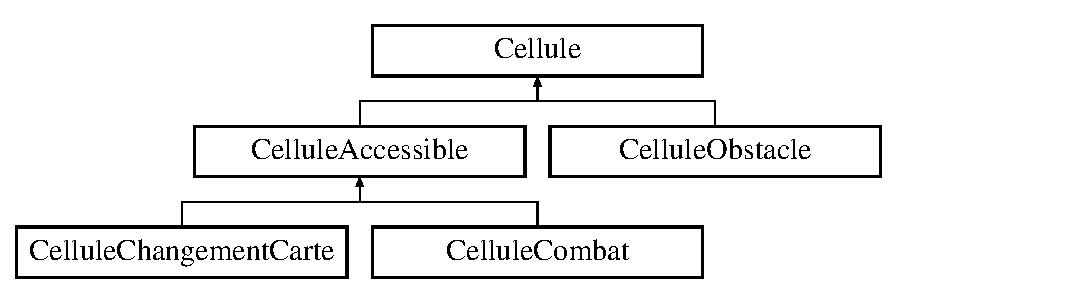
\includegraphics[height=3.000000cm]{classCellule}
\end{center}
\end{figure}
\subsection*{Public Member Functions}
\begin{DoxyCompactItemize}
\item 
\hypertarget{classCellule_a9f480ee53c2989d4630bc211626b0821}{\hyperlink{classCellule_a9f480ee53c2989d4630bc211626b0821}{Cellule} (string type\-Cell)}\label{classCellule_a9f480ee53c2989d4630bc211626b0821}

\begin{DoxyCompactList}\small\item\em Construit une \hyperlink{classCellule}{Cellule} de manière paramétrée. \end{DoxyCompactList}\item 
\hypertarget{classCellule_a41bfeb9bd31e275207cc61a0eb60ced1}{void \hyperlink{classCellule_a41bfeb9bd31e275207cc61a0eb60ced1}{set\-Action} (\hyperlink{classAction}{Action} $\ast$const action\-Cp)}\label{classCellule_a41bfeb9bd31e275207cc61a0eb60ced1}

\begin{DoxyCompactList}\small\item\em set l'action \end{DoxyCompactList}\item 
\hypertarget{classCellule_a28d417e43668d097610a695c3a667a28}{void \hyperlink{classCellule_a28d417e43668d097610a695c3a667a28}{set\-Type} (string const type\-Cp)}\label{classCellule_a28d417e43668d097610a695c3a667a28}

\begin{DoxyCompactList}\small\item\em set le type \end{DoxyCompactList}\item 
\hypertarget{classCellule_a3b037a2dea9fd2904c9d8a98af8148fa}{void \hyperlink{classCellule_a3b037a2dea9fd2904c9d8a98af8148fa}{lancer\-Action} () const }\label{classCellule_a3b037a2dea9fd2904c9d8a98af8148fa}

\begin{DoxyCompactList}\small\item\em Lance l'action et effectue les modifications nécessaires suite à cette action. \end{DoxyCompactList}\item 
virtual bool \hyperlink{classCellule_ac4e352254cf01f2d9f3666502f670f48}{est\-Accessible} ()=0
\begin{DoxyCompactList}\small\item\em Vérifie si la \hyperlink{classCellule}{Cellule} est Accessible ou non. \end{DoxyCompactList}\item 
string \hyperlink{classCellule_a856c03bf9534ed5fa00f076883a308c9}{get\-Type} () const 
\begin{DoxyCompactList}\small\item\em Getter type\-De\-Cellule. \end{DoxyCompactList}\item 
\hyperlink{classAction}{Action} $\ast$ \hyperlink{classCellule_af532f97ef0727572b8e0cf7afe265ccd}{get\-Action} () const 
\begin{DoxyCompactList}\small\item\em Getter \hyperlink{classAction}{Action}. \end{DoxyCompactList}\end{DoxyCompactItemize}


\subsection{Detailed Description}
\hyperlink{classCellule}{Cellule} composant les Zones du \hyperlink{classMonde}{Monde} où le joueur se déplace. 

\subsection{Member Function Documentation}
\hypertarget{classCellule_ac4e352254cf01f2d9f3666502f670f48}{\index{Cellule@{Cellule}!est\-Accessible@{est\-Accessible}}
\index{est\-Accessible@{est\-Accessible}!Cellule@{Cellule}}
\subsubsection[{est\-Accessible}]{\setlength{\rightskip}{0pt plus 5cm}bool Cellule\-::est\-Accessible (
\begin{DoxyParamCaption}
{}
\end{DoxyParamCaption}
)\hspace{0.3cm}{\ttfamily [pure virtual]}}}\label{classCellule_ac4e352254cf01f2d9f3666502f670f48}


Vérifie si la \hyperlink{classCellule}{Cellule} est Accessible ou non. 

Cette méthode est virtuelle car la classe est abstraite, elle sera implémentée dans les classes filles \begin{DoxyReturn}{Returns}
un booleen\-: vrai si la cellule est accessible, faux sinon 
\end{DoxyReturn}


Implemented in \hyperlink{classCelluleAccessible_a4250e365bbcb5a1b335d01bc3047cad5}{Cellule\-Accessible}, and \hyperlink{classCelluleObstacle_a8934b0a165d8b17c6710c3e42faf33f3}{Cellule\-Obstacle}.

\hypertarget{classCellule_af532f97ef0727572b8e0cf7afe265ccd}{\index{Cellule@{Cellule}!get\-Action@{get\-Action}}
\index{get\-Action@{get\-Action}!Cellule@{Cellule}}
\subsubsection[{get\-Action}]{\setlength{\rightskip}{0pt plus 5cm}{\bf Action} $\ast$ Cellule\-::get\-Action (
\begin{DoxyParamCaption}
{}
\end{DoxyParamCaption}
) const}}\label{classCellule_af532f97ef0727572b8e0cf7afe265ccd}


Getter \hyperlink{classAction}{Action}. 

\begin{DoxyReturn}{Returns}
action de la cellule 
\end{DoxyReturn}
\hypertarget{classCellule_a856c03bf9534ed5fa00f076883a308c9}{\index{Cellule@{Cellule}!get\-Type@{get\-Type}}
\index{get\-Type@{get\-Type}!Cellule@{Cellule}}
\subsubsection[{get\-Type}]{\setlength{\rightskip}{0pt plus 5cm}string Cellule\-::get\-Type (
\begin{DoxyParamCaption}
{}
\end{DoxyParamCaption}
) const}}\label{classCellule_a856c03bf9534ed5fa00f076883a308c9}


Getter type\-De\-Cellule. 

\begin{DoxyReturn}{Returns}
Type de cellule 
\end{DoxyReturn}


The documentation for this class was generated from the following files\-:\begin{DoxyCompactItemize}
\item 
/home/damien/\-Bureau/projetcpp\-\_\-gm42/source/src/\hyperlink{Cellule_8hpp}{Cellule.\-hpp}\item 
/home/damien/\-Bureau/projetcpp\-\_\-gm42/source/src/Cellule.\-cpp\end{DoxyCompactItemize}

\hypertarget{classCelluleAccessible}{\section{Cellule\-Accessible Class Reference}
\label{classCelluleAccessible}\index{Cellule\-Accessible@{Cellule\-Accessible}}
}


classe représentant les cellules du monde auquelles les personnages peuvent accéder  




{\ttfamily \#include $<$Cellule\-Accessible.\-hpp$>$}

Inheritance diagram for Cellule\-Accessible\-:\begin{figure}[H]
\begin{center}
\leavevmode
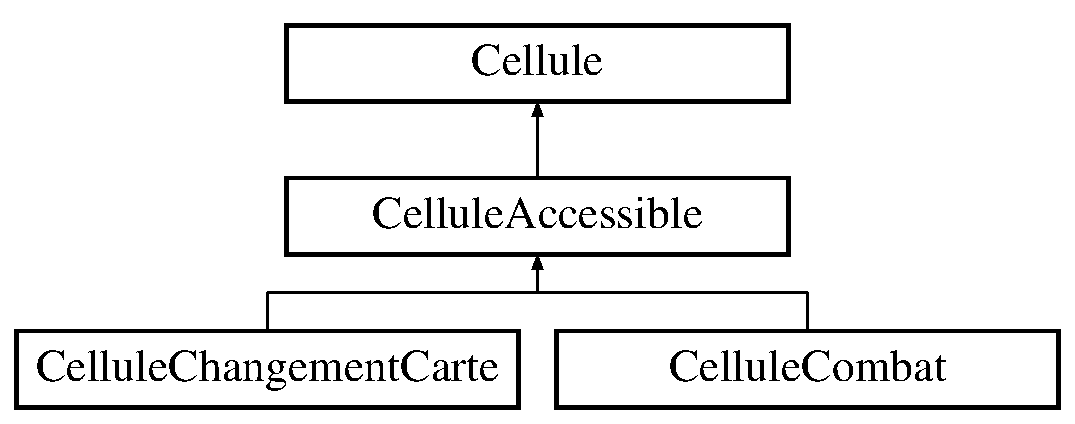
\includegraphics[height=3.000000cm]{classCelluleAccessible}
\end{center}
\end{figure}
\subsection*{Public Member Functions}
\begin{DoxyCompactItemize}
\item 
\hypertarget{classCelluleAccessible_a77f732f05d55c73361b9effe1428d3c6}{\hyperlink{classCelluleAccessible_a77f732f05d55c73361b9effe1428d3c6}{Cellule\-Accessible} ()}\label{classCelluleAccessible_a77f732f05d55c73361b9effe1428d3c6}

\begin{DoxyCompactList}\small\item\em Construit une \hyperlink{classCelluleAccessible}{Cellule\-Accessible}. \end{DoxyCompactList}\item 
\hyperlink{classCelluleAccessible_a0b70c93dc19145360f8064093dc4c204}{Cellule\-Accessible} (string type)
\begin{DoxyCompactList}\small\item\em Construit une \hyperlink{classCelluleAccessible}{Cellule\-Accessible}. \end{DoxyCompactList}\item 
\hyperlink{classCelluleAccessible_aaafd63dae10bff86a9602352c33a8d8a}{Cellule\-Accessible} (\hyperlink{classPersonnage}{Personnage} $\ast$perso)
\begin{DoxyCompactList}\small\item\em Construit une \hyperlink{classCelluleAccessible}{Cellule\-Accessible}. \end{DoxyCompactList}\item 
bool \hyperlink{classCelluleAccessible_a4250e365bbcb5a1b335d01bc3047cad5}{est\-Accessible} ()
\begin{DoxyCompactList}\small\item\em Vérifie si une classe est bien accessible. \end{DoxyCompactList}\item 
void \hyperlink{classCelluleAccessible_a83ccd256af299bf8d380611594c68548}{set\-Personnage} (\hyperlink{classPersonnage}{Personnage} $\ast$personnage)
\begin{DoxyCompactList}\small\item\em place un personnage sur une cellule \end{DoxyCompactList}\item 
\hyperlink{classPersonnage}{Personnage} $\ast$ \hyperlink{classCelluleAccessible_a2b7238e08a989a80b59022f77f6a22fa}{get\-Personnage} ()
\begin{DoxyCompactList}\small\item\em Getter de \hyperlink{classCellule}{Cellule} Accessible. \end{DoxyCompactList}\end{DoxyCompactItemize}


\subsection{Detailed Description}
classe représentant les cellules du monde auquelles les personnages peuvent accéder 

\subsection{Constructor \& Destructor Documentation}
\hypertarget{classCelluleAccessible_a0b70c93dc19145360f8064093dc4c204}{\index{Cellule\-Accessible@{Cellule\-Accessible}!Cellule\-Accessible@{Cellule\-Accessible}}
\index{Cellule\-Accessible@{Cellule\-Accessible}!CelluleAccessible@{Cellule\-Accessible}}
\subsubsection[{Cellule\-Accessible}]{\setlength{\rightskip}{0pt plus 5cm}Cellule\-Accessible\-::\-Cellule\-Accessible (
\begin{DoxyParamCaption}
\item[{string}]{type}
\end{DoxyParamCaption}
)}}\label{classCelluleAccessible_a0b70c93dc19145360f8064093dc4c204}


Construit une \hyperlink{classCelluleAccessible}{Cellule\-Accessible}. 


\begin{DoxyParams}{Parameters}
{\em type} & caractere du type a ajouter \\
\hline
\end{DoxyParams}
\hypertarget{classCelluleAccessible_aaafd63dae10bff86a9602352c33a8d8a}{\index{Cellule\-Accessible@{Cellule\-Accessible}!Cellule\-Accessible@{Cellule\-Accessible}}
\index{Cellule\-Accessible@{Cellule\-Accessible}!CelluleAccessible@{Cellule\-Accessible}}
\subsubsection[{Cellule\-Accessible}]{\setlength{\rightskip}{0pt plus 5cm}Cellule\-Accessible\-::\-Cellule\-Accessible (
\begin{DoxyParamCaption}
\item[{{\bf Personnage} $\ast$}]{perso}
\end{DoxyParamCaption}
)}}\label{classCelluleAccessible_aaafd63dae10bff86a9602352c33a8d8a}


Construit une \hyperlink{classCelluleAccessible}{Cellule\-Accessible}. 


\begin{DoxyParams}{Parameters}
{\em perso} & \-: \hyperlink{classPersonnage}{Personnage} a affecter \\
\hline
\end{DoxyParams}


\subsection{Member Function Documentation}
\hypertarget{classCelluleAccessible_a4250e365bbcb5a1b335d01bc3047cad5}{\index{Cellule\-Accessible@{Cellule\-Accessible}!est\-Accessible@{est\-Accessible}}
\index{est\-Accessible@{est\-Accessible}!CelluleAccessible@{Cellule\-Accessible}}
\subsubsection[{est\-Accessible}]{\setlength{\rightskip}{0pt plus 5cm}bool Cellule\-Accessible\-::est\-Accessible (
\begin{DoxyParamCaption}
{}
\end{DoxyParamCaption}
)\hspace{0.3cm}{\ttfamily [virtual]}}}\label{classCelluleAccessible_a4250e365bbcb5a1b335d01bc3047cad5}


Vérifie si une classe est bien accessible. 

\begin{DoxyReturn}{Returns}
un booleen vrai si la classe est accessible, faux sinon 
\end{DoxyReturn}


Implements \hyperlink{classCellule_ac4e352254cf01f2d9f3666502f670f48}{Cellule}.

\hypertarget{classCelluleAccessible_a2b7238e08a989a80b59022f77f6a22fa}{\index{Cellule\-Accessible@{Cellule\-Accessible}!get\-Personnage@{get\-Personnage}}
\index{get\-Personnage@{get\-Personnage}!CelluleAccessible@{Cellule\-Accessible}}
\subsubsection[{get\-Personnage}]{\setlength{\rightskip}{0pt plus 5cm}Cellule\-Accessible\-::get\-Personnage (
\begin{DoxyParamCaption}
{}
\end{DoxyParamCaption}
)}}\label{classCelluleAccessible_a2b7238e08a989a80b59022f77f6a22fa}


Getter de \hyperlink{classCellule}{Cellule} Accessible. 

\begin{DoxyReturn}{Returns}
personnage \-: pointeur sur un personnage 
\end{DoxyReturn}
\hypertarget{classCelluleAccessible_a83ccd256af299bf8d380611594c68548}{\index{Cellule\-Accessible@{Cellule\-Accessible}!set\-Personnage@{set\-Personnage}}
\index{set\-Personnage@{set\-Personnage}!CelluleAccessible@{Cellule\-Accessible}}
\subsubsection[{set\-Personnage}]{\setlength{\rightskip}{0pt plus 5cm}void Cellule\-Accessible\-::set\-Personnage (
\begin{DoxyParamCaption}
\item[{{\bf Personnage} $\ast$}]{personnage}
\end{DoxyParamCaption}
)}}\label{classCelluleAccessible_a83ccd256af299bf8d380611594c68548}


place un personnage sur une cellule 


\begin{DoxyParams}{Parameters}
{\em personnage} & \-: pointeur sur personnage à placer sur la cellule \\
\hline
\end{DoxyParams}


The documentation for this class was generated from the following files\-:\begin{DoxyCompactItemize}
\item 
/home/damien/\-Bureau/projetcpp\-\_\-gm42/source/src/\hyperlink{CelluleAccessible_8hpp}{Cellule\-Accessible.\-hpp}\item 
/home/damien/\-Bureau/projetcpp\-\_\-gm42/source/src/Cellule\-Accessible.\-cpp\end{DoxyCompactItemize}

\hypertarget{classCelluleChangementCarte}{\section{Cellule\-Changement\-Carte Class Reference}
\label{classCelluleChangementCarte}\index{Cellule\-Changement\-Carte@{Cellule\-Changement\-Carte}}
}


\hyperlink{classCelluleAccessible}{Cellule\-Accessible} permettant d'engager un Changement\-Carte.  




{\ttfamily \#include $<$Cellule\-Changement\-Carte.\-hpp$>$}

Inheritance diagram for Cellule\-Changement\-Carte\-:\begin{figure}[H]
\begin{center}
\leavevmode
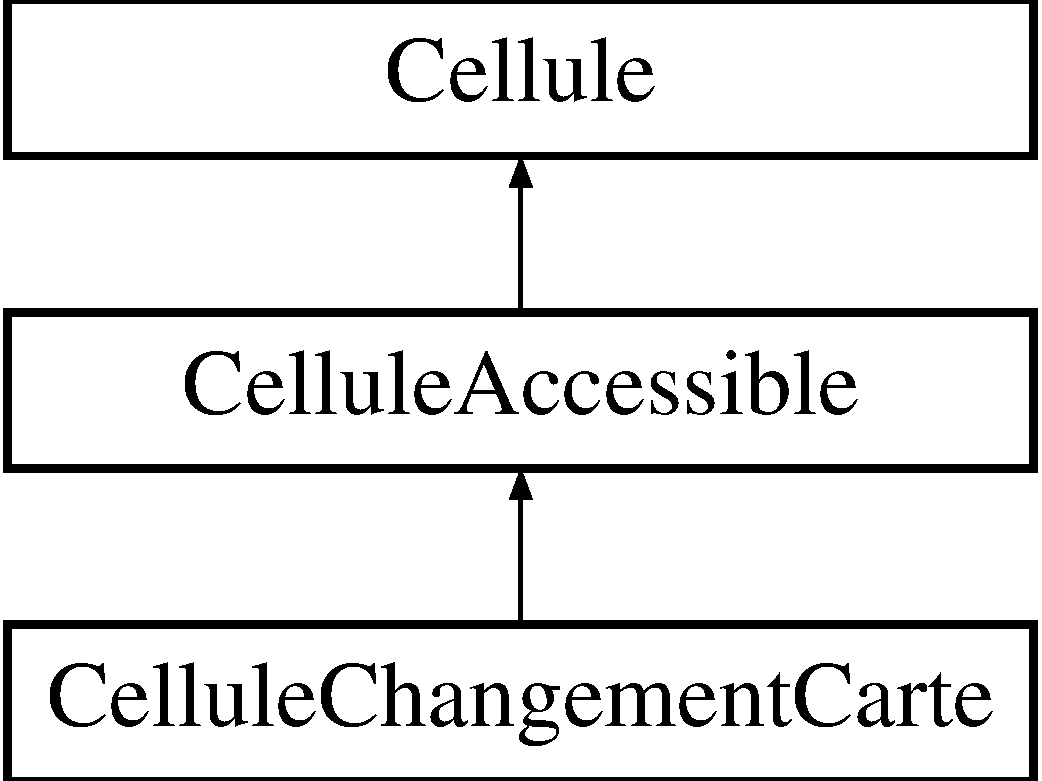
\includegraphics[height=3.000000cm]{classCelluleChangementCarte}
\end{center}
\end{figure}
\subsection*{Public Member Functions}
\begin{DoxyCompactItemize}
\item 
\hypertarget{classCelluleChangementCarte_a8c43a2087ebbfff9ff5346af569e4906}{\hyperlink{classCelluleChangementCarte_a8c43a2087ebbfff9ff5346af569e4906}{Cellule\-Changement\-Carte} (\hyperlink{classCarte}{Carte} $\ast$carte\-Init, \hyperlink{classCarte}{Carte} $\ast$carte\-Dest, \hyperlink{classCoordonnees}{Coordonnees} coord\-Init, \hyperlink{classCoordonnees}{Coordonnees} coord\-Dest)}\label{classCelluleChangementCarte_a8c43a2087ebbfff9ff5346af569e4906}

\begin{DoxyCompactList}\small\item\em Construit une \hyperlink{classCellule}{Cellule}. \end{DoxyCompactList}\end{DoxyCompactItemize}


\subsection{Detailed Description}
\hyperlink{classCelluleAccessible}{Cellule\-Accessible} permettant d'engager un Changement\-Carte. 

The documentation for this class was generated from the following files\-:\begin{DoxyCompactItemize}
\item 
/home/damien/\-Bureau/projetcpp\-\_\-gm42/source/src/\hyperlink{CelluleChangementCarte_8hpp}{Cellule\-Changement\-Carte.\-hpp}\item 
/home/damien/\-Bureau/projetcpp\-\_\-gm42/source/src/Cellule\-Changement\-Carte.\-cpp\end{DoxyCompactItemize}

\hypertarget{classCelluleCombat}{\section{Cellule\-Combat Class Reference}
\label{classCelluleCombat}\index{Cellule\-Combat@{Cellule\-Combat}}
}


\hyperlink{classCelluleAccessible}{Cellule\-Accessible} permettant d'engager un \hyperlink{classCombat}{Combat}.  




{\ttfamily \#include $<$Cellule\-Combat.\-hpp$>$}

Inheritance diagram for Cellule\-Combat\-:\begin{figure}[H]
\begin{center}
\leavevmode
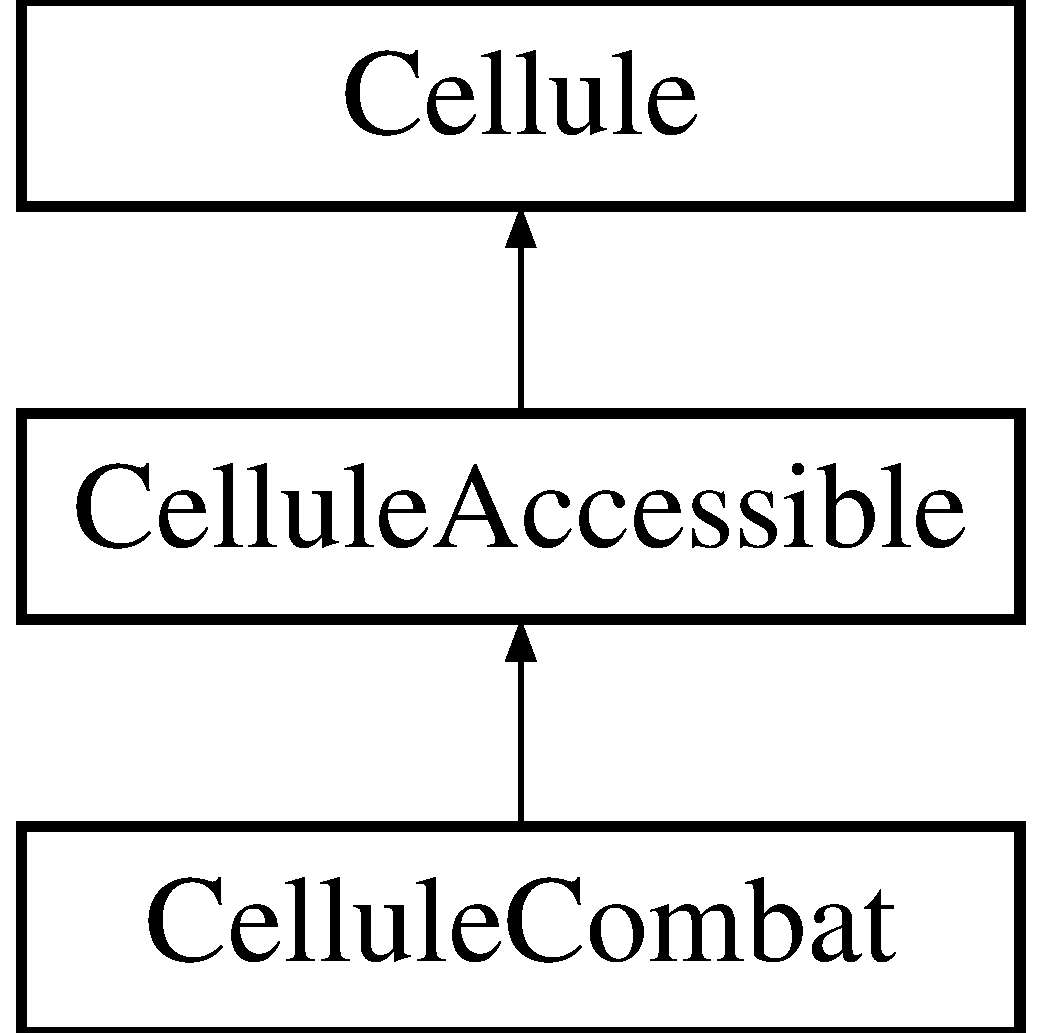
\includegraphics[height=3.000000cm]{classCelluleCombat}
\end{center}
\end{figure}
\subsection*{Public Member Functions}
\begin{DoxyCompactItemize}
\item 
\hypertarget{classCelluleCombat_a53dd066618a86b4986ae54ff49d64b3d}{\hyperlink{classCelluleCombat_a53dd066618a86b4986ae54ff49d64b3d}{Cellule\-Combat} (\hyperlink{classPersonnage}{Personnage} $\ast$adv)}\label{classCelluleCombat_a53dd066618a86b4986ae54ff49d64b3d}

\begin{DoxyCompactList}\small\item\em Construit une \hyperlink{classCellule}{Cellule}. \end{DoxyCompactList}\end{DoxyCompactItemize}


\subsection{Detailed Description}
\hyperlink{classCelluleAccessible}{Cellule\-Accessible} permettant d'engager un \hyperlink{classCombat}{Combat}. 

The documentation for this class was generated from the following files\-:\begin{DoxyCompactItemize}
\item 
/home/damien/\-Bureau/projetcpp\-\_\-gm42/source/src/\hyperlink{CelluleCombat_8hpp}{Cellule\-Combat.\-hpp}\item 
/home/damien/\-Bureau/projetcpp\-\_\-gm42/source/src/Cellule\-Combat.\-cpp\end{DoxyCompactItemize}

\hypertarget{classCelluleObstacle}{\section{Cellule\-Obstacle Class Reference}
\label{classCelluleObstacle}\index{Cellule\-Obstacle@{Cellule\-Obstacle}}
}


\hyperlink{classCellule}{Cellule} contenant un obstacle.  




{\ttfamily \#include $<$Cellule\-Obstacle.\-hpp$>$}

Inheritance diagram for Cellule\-Obstacle\-:\begin{figure}[H]
\begin{center}
\leavevmode
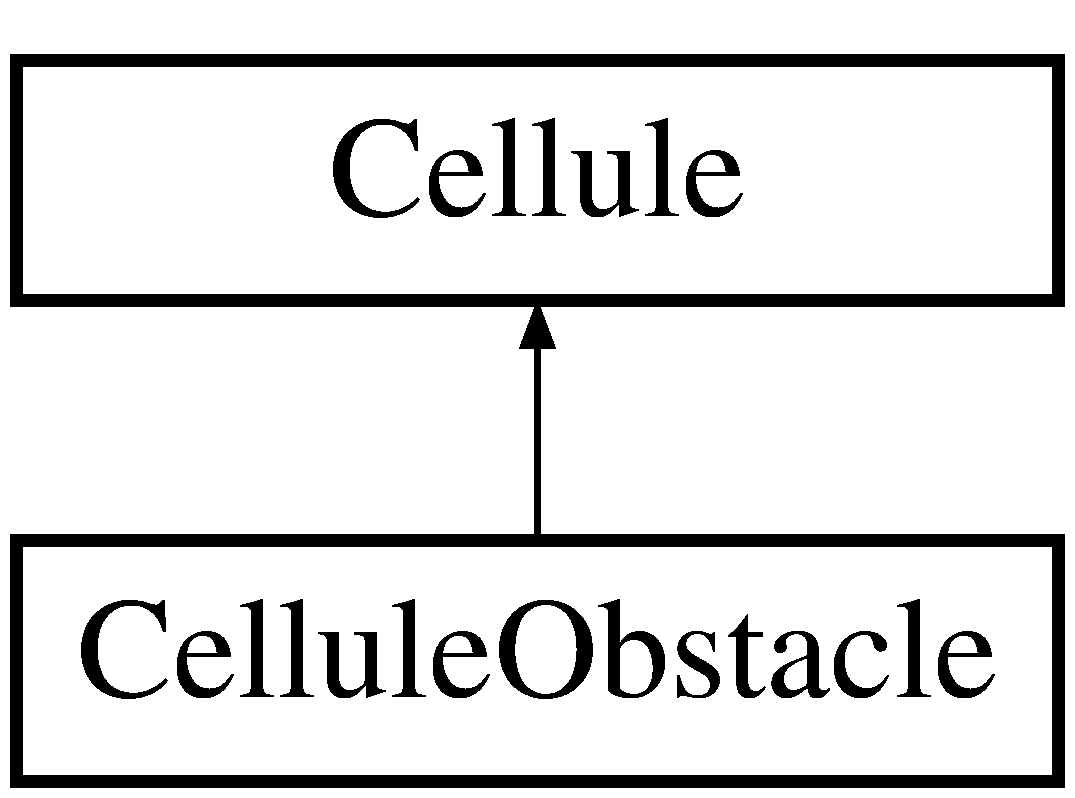
\includegraphics[height=2.000000cm]{classCelluleObstacle}
\end{center}
\end{figure}
\subsection*{Public Member Functions}
\begin{DoxyCompactItemize}
\item 
\hypertarget{classCelluleObstacle_a03257715748cbe82a95fe36af7ab51a5}{\hyperlink{classCelluleObstacle_a03257715748cbe82a95fe36af7ab51a5}{Cellule\-Obstacle} ()}\label{classCelluleObstacle_a03257715748cbe82a95fe36af7ab51a5}

\begin{DoxyCompactList}\small\item\em Constructeur de notre classe. \end{DoxyCompactList}\item 
bool \hyperlink{classCelluleObstacle_a8934b0a165d8b17c6710c3e42faf33f3}{est\-Accessible} ()
\begin{DoxyCompactList}\small\item\em vérifie si une case est accessible \end{DoxyCompactList}\end{DoxyCompactItemize}


\subsection{Detailed Description}
\hyperlink{classCellule}{Cellule} contenant un obstacle. 

Classe générant une cellule contenant un obstacle sur laquelle le joueur ne peut donc pas accéder 

\subsection{Member Function Documentation}
\hypertarget{classCelluleObstacle_a8934b0a165d8b17c6710c3e42faf33f3}{\index{Cellule\-Obstacle@{Cellule\-Obstacle}!est\-Accessible@{est\-Accessible}}
\index{est\-Accessible@{est\-Accessible}!CelluleObstacle@{Cellule\-Obstacle}}
\subsubsection[{est\-Accessible}]{\setlength{\rightskip}{0pt plus 5cm}bool Cellule\-Obstacle\-::est\-Accessible (
\begin{DoxyParamCaption}
{}
\end{DoxyParamCaption}
)\hspace{0.3cm}{\ttfamily [virtual]}}}\label{classCelluleObstacle_a8934b0a165d8b17c6710c3e42faf33f3}


vérifie si une case est accessible 

\begin{DoxyReturn}{Returns}
retourne faux car la cellule contient un obstacle 
\end{DoxyReturn}


Implements \hyperlink{classCellule_ac4e352254cf01f2d9f3666502f670f48}{Cellule}.



The documentation for this class was generated from the following files\-:\begin{DoxyCompactItemize}
\item 
/home/damien/\-Bureau/projetcpp\-\_\-gm42/source/src/\hyperlink{CelluleObstacle_8hpp}{Cellule\-Obstacle.\-hpp}\item 
/home/damien/\-Bureau/projetcpp\-\_\-gm42/source/src/Cellule\-Obstacle.\-cpp\end{DoxyCompactItemize}

\hypertarget{classCombat}{\section{Combat Class Reference}
\label{classCombat}\index{Combat@{Combat}}
}


\hyperlink{classCombat}{Combat} à deux joueurs.  




{\ttfamily \#include $<$Combat.\-hpp$>$}

Inheritance diagram for Combat\-:\begin{figure}[H]
\begin{center}
\leavevmode
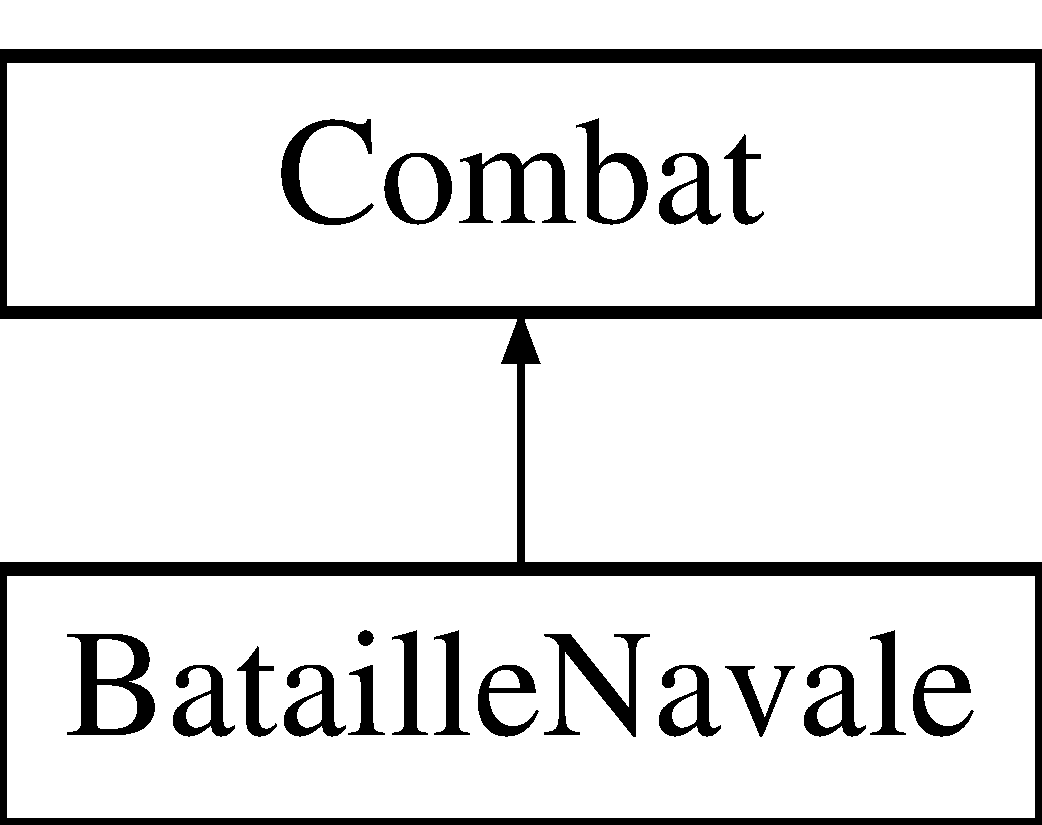
\includegraphics[height=2.000000cm]{classCombat}
\end{center}
\end{figure}
\subsection*{Public Member Functions}
\begin{DoxyCompactItemize}
\item 
virtual \hyperlink{classPersonnage}{Personnage} $\ast$ \hyperlink{classCombat_a5b480832873d1bf4e8a91f1c7054e646}{retourner\-Gagnant} (\hyperlink{classPersonnage}{Personnage} $\ast$joueur1, \hyperlink{classPersonnage}{Personnage} $\ast$joueur2)=0
\begin{DoxyCompactList}\small\item\em Retourner Gagnant. \end{DoxyCompactList}\end{DoxyCompactItemize}


\subsection{Detailed Description}
\hyperlink{classCombat}{Combat} à deux joueurs. 

Classe permettant la gestion d'un combat à deux joueurs avec les fonctions génériques qui reviennent pour tous les combats. 

\subsection{Member Function Documentation}
\hypertarget{classCombat_a5b480832873d1bf4e8a91f1c7054e646}{\index{Combat@{Combat}!retourner\-Gagnant@{retourner\-Gagnant}}
\index{retourner\-Gagnant@{retourner\-Gagnant}!Combat@{Combat}}
\subsubsection[{retourner\-Gagnant}]{\setlength{\rightskip}{0pt plus 5cm}{\bf Personnage} Combat\-::retourner\-Gagnant (
\begin{DoxyParamCaption}
\item[{{\bf Personnage} $\ast$}]{joueur1, }
\item[{{\bf Personnage} $\ast$}]{joueur2}
\end{DoxyParamCaption}
)\hspace{0.3cm}{\ttfamily [pure virtual]}}}\label{classCombat_a5b480832873d1bf4e8a91f1c7054e646}


Retourner Gagnant. 


\begin{DoxyParams}{Parameters}
{\em joueur1} & représente le premier joueur initial de notre combat \\
\hline
{\em joueur2} & représente le deuxième joueur initial de notre combat\\
\hline
\end{DoxyParams}
Méthode qui renvoie le gagnant du combat \begin{DoxyReturn}{Returns}
un personnage correspondant au gagnant et null si la partie n'est pas finie 
\end{DoxyReturn}


Implemented in \hyperlink{classBatailleNavale_acff7cd9717a2ed3084b232d95ea9042a}{Bataille\-Navale}.



The documentation for this class was generated from the following file\-:\begin{DoxyCompactItemize}
\item 
/home/damien/\-Bureau/projetcpp\-\_\-gm42/source/src/\hyperlink{Combat_8hpp}{Combat.\-hpp}\end{DoxyCompactItemize}

\hypertarget{classControleur}{\section{Controleur Class Reference}
\label{classControleur}\index{Controleur@{Controleur}}
}


\hyperlink{classControleur}{Controleur} de notre partie.  


\subsection*{Public Member Functions}
\begin{DoxyCompactItemize}
\item 
\hyperlink{classControleur_a2b3859d8cb6bd1c0407be722962470bd}{Controleur} ()
\begin{DoxyCompactList}\small\item\em Constructeur. \end{DoxyCompactList}\item 
void \hyperlink{classControleur_a6662763d2f3225edcc192ccf19836a80}{tour\-De\-Jeu} ()
\begin{DoxyCompactList}\small\item\em tour De \hyperlink{classJeu}{Jeu} \end{DoxyCompactList}\item 
\hypertarget{classControleur_afe801f272c1edfa0a237695235be03ec}{void \hyperlink{classControleur_afe801f272c1edfa0a237695235be03ec}{lancer\-Jeu} ()}\label{classControleur_afe801f272c1edfa0a237695235be03ec}

\begin{DoxyCompactList}\small\item\em lancement du jeu Tant que la partie n'est pas terminée, on continue à faire des tours de jeu \end{DoxyCompactList}\item 
void \hyperlink{classControleur_abdb6d62a15b5446b0b9dfad333690d85}{action\-Bataille\-Navale} ()
\begin{DoxyCompactList}\small\item\em lancement de la bataille navale \end{DoxyCompactList}\item 
void \hyperlink{classControleur_a5b414b0306b79e3978c00f70089d796d}{tour\-De\-Jeu\-Bataille\-Navale} ()
\begin{DoxyCompactList}\small\item\em tour de jeu Bataille Navale \end{DoxyCompactList}\end{DoxyCompactItemize}


\subsection{Detailed Description}
\hyperlink{classControleur}{Controleur} de notre partie. 

Classe \hyperlink{classControleur}{Controleur} permettant la connexion entre notre modèle et notre vue Le \hyperlink{classControleur}{Controleur} contient le jeu courant et la bataille navale en cours 

\subsection{Constructor \& Destructor Documentation}
\hypertarget{classControleur_a2b3859d8cb6bd1c0407be722962470bd}{\index{Controleur@{Controleur}!Controleur@{Controleur}}
\index{Controleur@{Controleur}!Controleur@{Controleur}}
\subsubsection[{Controleur}]{\setlength{\rightskip}{0pt plus 5cm}Controleur\-::\-Controleur (
\begin{DoxyParamCaption}
{}
\end{DoxyParamCaption}
)}}\label{classControleur_a2b3859d8cb6bd1c0407be722962470bd}


Constructeur. 

Constructeur de notre \hyperlink{classControleur}{Controleur} On crée un nouveau jeu, et une I\-H\-M ayant comme paramètre ce jeu 

\subsection{Member Function Documentation}
\hypertarget{classControleur_abdb6d62a15b5446b0b9dfad333690d85}{\index{Controleur@{Controleur}!action\-Bataille\-Navale@{action\-Bataille\-Navale}}
\index{action\-Bataille\-Navale@{action\-Bataille\-Navale}!Controleur@{Controleur}}
\subsubsection[{action\-Bataille\-Navale}]{\setlength{\rightskip}{0pt plus 5cm}void Controleur\-::action\-Bataille\-Navale (
\begin{DoxyParamCaption}
{}
\end{DoxyParamCaption}
)}}\label{classControleur_abdb6d62a15b5446b0b9dfad333690d85}


lancement de la bataille navale 

Tant que la partie n'est pas terminée, on continue à faire des tours de jeu \hypertarget{classControleur_a6662763d2f3225edcc192ccf19836a80}{\index{Controleur@{Controleur}!tour\-De\-Jeu@{tour\-De\-Jeu}}
\index{tour\-De\-Jeu@{tour\-De\-Jeu}!Controleur@{Controleur}}
\subsubsection[{tour\-De\-Jeu}]{\setlength{\rightskip}{0pt plus 5cm}void Controleur\-::tour\-De\-Jeu (
\begin{DoxyParamCaption}
{}
\end{DoxyParamCaption}
)}}\label{classControleur_a6662763d2f3225edcc192ccf19836a80}


tour De \hyperlink{classJeu}{Jeu} 

Affiche la carte, saisie, joue le déplacement saisi, et effectue l'action en cours \hypertarget{classControleur_a5b414b0306b79e3978c00f70089d796d}{\index{Controleur@{Controleur}!tour\-De\-Jeu\-Bataille\-Navale@{tour\-De\-Jeu\-Bataille\-Navale}}
\index{tour\-De\-Jeu\-Bataille\-Navale@{tour\-De\-Jeu\-Bataille\-Navale}!Controleur@{Controleur}}
\subsubsection[{tour\-De\-Jeu\-Bataille\-Navale}]{\setlength{\rightskip}{0pt plus 5cm}void Controleur\-::tour\-De\-Jeu\-Bataille\-Navale (
\begin{DoxyParamCaption}
{}
\end{DoxyParamCaption}
)}}\label{classControleur_a5b414b0306b79e3978c00f70089d796d}


tour de jeu Bataille Navale 

Tant que la bataille navale n'est pas terminée, on continue à faire des tours de bataille navale 

The documentation for this class was generated from the following files\-:\begin{DoxyCompactItemize}
\item 
/home/damien/\-Bureau/projetcpp\-\_\-gm42/source/src/\hyperlink{Controleur_8hpp}{Controleur.\-hpp}\item 
/home/damien/\-Bureau/projetcpp\-\_\-gm42/source/src/Controleur.\-cpp\end{DoxyCompactItemize}

\hypertarget{classControleurBN}{\section{Controleur\-B\-N Class Reference}
\label{classControleurBN}\index{Controleur\-B\-N@{Controleur\-B\-N}}
}


\hyperlink{classControleur}{Controleur} de notre B\-N.  


\subsection*{Public Member Functions}
\begin{DoxyCompactItemize}
\item 
\hyperlink{classControleurBN_ac135f946e0783bc8afd63bb6b1ba0ed6}{Controleur\-B\-N} (\hyperlink{classBatailleNavale}{Bataille\-Navale} $\ast$batnav)
\begin{DoxyCompactList}\small\item\em Constructeur. \end{DoxyCompactList}\item 
void \hyperlink{classControleurBN_a459747029d8787d21c2063c718771c97}{action\-Bataille\-Navale} ()
\begin{DoxyCompactList}\small\item\em lancement de la bataille navale \end{DoxyCompactList}\item 
void \hyperlink{classControleurBN_a41ac895ee55442bf38ed4997298c4503}{tour\-De\-Jeu\-Bataille\-Navale} (\hyperlink{classIHMBN}{I\-H\-M\-B\-N} $\ast$ihm\-B\-N)
\begin{DoxyCompactList}\small\item\em tour de jeu Bataille Navale \end{DoxyCompactList}\end{DoxyCompactItemize}


\subsection{Detailed Description}
\hyperlink{classControleur}{Controleur} de notre B\-N. 

Classe \hyperlink{classControleur}{Controleur} permettant la connexion entre notre modèle et notre vue du côté B\-N 

\subsection{Constructor \& Destructor Documentation}
\hypertarget{classControleurBN_ac135f946e0783bc8afd63bb6b1ba0ed6}{\index{Controleur\-B\-N@{Controleur\-B\-N}!Controleur\-B\-N@{Controleur\-B\-N}}
\index{Controleur\-B\-N@{Controleur\-B\-N}!ControleurBN@{Controleur\-B\-N}}
\subsubsection[{Controleur\-B\-N}]{\setlength{\rightskip}{0pt plus 5cm}Controleur\-B\-N\-::\-Controleur\-B\-N (
\begin{DoxyParamCaption}
\item[{{\bf Bataille\-Navale} $\ast$}]{batnav}
\end{DoxyParamCaption}
)}}\label{classControleurBN_ac135f946e0783bc8afd63bb6b1ba0ed6}


Constructeur. 

Constructeur de notre \hyperlink{classControleur}{Controleur} On crée un controleur B\-N 
\begin{DoxyParams}{Parameters}
{\em batnav} & \-: combat d'entree \\
\hline
\end{DoxyParams}


\subsection{Member Function Documentation}
\hypertarget{classControleurBN_a459747029d8787d21c2063c718771c97}{\index{Controleur\-B\-N@{Controleur\-B\-N}!action\-Bataille\-Navale@{action\-Bataille\-Navale}}
\index{action\-Bataille\-Navale@{action\-Bataille\-Navale}!ControleurBN@{Controleur\-B\-N}}
\subsubsection[{action\-Bataille\-Navale}]{\setlength{\rightskip}{0pt plus 5cm}void Controleur\-B\-N\-::action\-Bataille\-Navale (
\begin{DoxyParamCaption}
{}
\end{DoxyParamCaption}
)}}\label{classControleurBN_a459747029d8787d21c2063c718771c97}


lancement de la bataille navale 

Tant que la partie n'est pas terminée, on continue à faire des tours de jeu \hypertarget{classControleurBN_a41ac895ee55442bf38ed4997298c4503}{\index{Controleur\-B\-N@{Controleur\-B\-N}!tour\-De\-Jeu\-Bataille\-Navale@{tour\-De\-Jeu\-Bataille\-Navale}}
\index{tour\-De\-Jeu\-Bataille\-Navale@{tour\-De\-Jeu\-Bataille\-Navale}!ControleurBN@{Controleur\-B\-N}}
\subsubsection[{tour\-De\-Jeu\-Bataille\-Navale}]{\setlength{\rightskip}{0pt plus 5cm}void Controleur\-B\-N\-::tour\-De\-Jeu\-Bataille\-Navale (
\begin{DoxyParamCaption}
\item[{{\bf I\-H\-M\-B\-N} $\ast$}]{ihm\-B\-N}
\end{DoxyParamCaption}
)}}\label{classControleurBN_a41ac895ee55442bf38ed4997298c4503}


tour de jeu Bataille Navale 

Tant que la bataille navale n'est pas terminée, on continue à faire des tours de bataille navale 
\begin{DoxyParams}{Parameters}
{\em ihm\-B\-N} & \-: pointeur sur I\-H\-M \\
\hline
\end{DoxyParams}


The documentation for this class was generated from the following files\-:\begin{DoxyCompactItemize}
\item 
/home/damien/\-Bureau/projetcpp\-\_\-gm42/source/src/\hyperlink{ControleurBN_8hpp}{Controleur\-B\-N.\-hpp}\item 
/home/damien/\-Bureau/projetcpp\-\_\-gm42/source/src/Controleur\-B\-N.\-cpp\end{DoxyCompactItemize}

\hypertarget{classCoordonnees}{\section{Coordonnees Class Reference}
\label{classCoordonnees}\index{Coordonnees@{Coordonnees}}
}


\hyperlink{classCoordonnees}{Coordonnees} sur une carte.  




{\ttfamily \#include $<$Coordonnees.\-hpp$>$}

\subsection*{Public Member Functions}
\begin{DoxyCompactItemize}
\item 
\hyperlink{classCoordonnees_a6ec732bf5bf8b43d458340b9f2be9edb}{Coordonnees} (const int abs, const int ord)
\begin{DoxyCompactList}\small\item\em Contructeur paramétré \end{DoxyCompactList}\item 
\hyperlink{classCoordonnees_a30d6f3b61bfb6762709f9ae7c62dc4b7}{Coordonnees} (const \hyperlink{classCoordonnees}{Coordonnees} \&coord)
\begin{DoxyCompactList}\small\item\em Contructeur par recopie. \end{DoxyCompactList}\item 
\hypertarget{classCoordonnees_a0f5af89bc4c49a5cf265c8362567cbe1}{void \hyperlink{classCoordonnees_a0f5af89bc4c49a5cf265c8362567cbe1}{copy} (const \hyperlink{classCoordonnees}{Coordonnees} coordcp)}\label{classCoordonnees_a0f5af89bc4c49a5cf265c8362567cbe1}

\begin{DoxyCompactList}\small\item\em Copieur de coordonnes. \end{DoxyCompactList}\item 
int \hyperlink{classCoordonnees_ad265ffa4100fe0abfab4f85b0f5a1ad9}{get\-Abscisse} () const 
\begin{DoxyCompactList}\small\item\em getteur de l'abscisse \end{DoxyCompactList}\item 
int \hyperlink{classCoordonnees_aa85ba028b69971541d3f236d7abaa132}{get\-Ordonnee} () const 
\begin{DoxyCompactList}\small\item\em getteur de l'ordonnée \end{DoxyCompactList}\item 
void \hyperlink{classCoordonnees_a3755536bdb242d6d78fc486423007448}{set\-Ordonnee} (const int o)
\begin{DoxyCompactList}\small\item\em setteur de l'ordonnée \end{DoxyCompactList}\item 
void \hyperlink{classCoordonnees_abf053f302f5b1f25af39036d5a85a80a}{set\-Abscisse} (const int a)
\begin{DoxyCompactList}\small\item\em setteur de l'abscisse \end{DoxyCompactList}\item 
bool \hyperlink{classCoordonnees_af5bf5f6a84b87f6d980669f583167a8a}{coordonnees\-Vides} ()
\begin{DoxyCompactList}\small\item\em vérifie si la coordonnee est vide ou non(créé par un I\-A ou non) \end{DoxyCompactList}\end{DoxyCompactItemize}


\subsection{Detailed Description}
\hyperlink{classCoordonnees}{Coordonnees} sur une carte. 

Classe \hyperlink{classCoordonnees}{Coordonnees} représentant les coordonnées de notre joueur ou de notre obstacle sur la carte 

\subsection{Constructor \& Destructor Documentation}
\hypertarget{classCoordonnees_a6ec732bf5bf8b43d458340b9f2be9edb}{\index{Coordonnees@{Coordonnees}!Coordonnees@{Coordonnees}}
\index{Coordonnees@{Coordonnees}!Coordonnees@{Coordonnees}}
\subsubsection[{Coordonnees}]{\setlength{\rightskip}{0pt plus 5cm}Coordonnees\-::\-Coordonnees (
\begin{DoxyParamCaption}
\item[{const int}]{abs, }
\item[{const int}]{ord}
\end{DoxyParamCaption}
)}}\label{classCoordonnees_a6ec732bf5bf8b43d458340b9f2be9edb}


Contructeur paramétré 

Constructeur permettant d'instancier une coordonnée avec une abscisse et une ordonnée 
\begin{DoxyParams}{Parameters}
{\em abs} & entier correspondant à l'abscisse \\
\hline
{\em ord} & entier correspondant à l'ordonnée \\
\hline
\end{DoxyParams}
\hypertarget{classCoordonnees_a30d6f3b61bfb6762709f9ae7c62dc4b7}{\index{Coordonnees@{Coordonnees}!Coordonnees@{Coordonnees}}
\index{Coordonnees@{Coordonnees}!Coordonnees@{Coordonnees}}
\subsubsection[{Coordonnees}]{\setlength{\rightskip}{0pt plus 5cm}Coordonnees\-::\-Coordonnees (
\begin{DoxyParamCaption}
\item[{const {\bf Coordonnees} \&}]{coord}
\end{DoxyParamCaption}
)}}\label{classCoordonnees_a30d6f3b61bfb6762709f9ae7c62dc4b7}


Contructeur par recopie. 

Constructeur permettant d'instancier une coordonnée avec instance de \hyperlink{classCoordonnees}{Coordonnees} 
\begin{DoxyParams}{Parameters}
{\em coord} & \-: \hyperlink{classCoordonnees}{Coordonnees} a recopier \\
\hline
\end{DoxyParams}


\subsection{Member Function Documentation}
\hypertarget{classCoordonnees_af5bf5f6a84b87f6d980669f583167a8a}{\index{Coordonnees@{Coordonnees}!coordonnees\-Vides@{coordonnees\-Vides}}
\index{coordonnees\-Vides@{coordonnees\-Vides}!Coordonnees@{Coordonnees}}
\subsubsection[{coordonnees\-Vides}]{\setlength{\rightskip}{0pt plus 5cm}{\bf Coordonnees} Coordonnees\-::coordonnees\-Vides (
\begin{DoxyParamCaption}
{}
\end{DoxyParamCaption}
)}}\label{classCoordonnees_af5bf5f6a84b87f6d980669f583167a8a}


vérifie si la coordonnee est vide ou non(créé par un I\-A ou non) 

\begin{DoxyReturn}{Returns}
bool true si la coordonnee est vide, false sinon 
\end{DoxyReturn}
\hypertarget{classCoordonnees_ad265ffa4100fe0abfab4f85b0f5a1ad9}{\index{Coordonnees@{Coordonnees}!get\-Abscisse@{get\-Abscisse}}
\index{get\-Abscisse@{get\-Abscisse}!Coordonnees@{Coordonnees}}
\subsubsection[{get\-Abscisse}]{\setlength{\rightskip}{0pt plus 5cm}int Coordonnees\-::get\-Abscisse (
\begin{DoxyParamCaption}
{}
\end{DoxyParamCaption}
) const}}\label{classCoordonnees_ad265ffa4100fe0abfab4f85b0f5a1ad9}


getteur de l'abscisse 

\begin{DoxyReturn}{Returns}
entier correspondant à l'abscisse 
\end{DoxyReturn}
\hypertarget{classCoordonnees_aa85ba028b69971541d3f236d7abaa132}{\index{Coordonnees@{Coordonnees}!get\-Ordonnee@{get\-Ordonnee}}
\index{get\-Ordonnee@{get\-Ordonnee}!Coordonnees@{Coordonnees}}
\subsubsection[{get\-Ordonnee}]{\setlength{\rightskip}{0pt plus 5cm}int Coordonnees\-::get\-Ordonnee (
\begin{DoxyParamCaption}
{}
\end{DoxyParamCaption}
) const}}\label{classCoordonnees_aa85ba028b69971541d3f236d7abaa132}


getteur de l'ordonnée 

\begin{DoxyReturn}{Returns}
entier correspondant à l'ordonnée 
\end{DoxyReturn}
\hypertarget{classCoordonnees_abf053f302f5b1f25af39036d5a85a80a}{\index{Coordonnees@{Coordonnees}!set\-Abscisse@{set\-Abscisse}}
\index{set\-Abscisse@{set\-Abscisse}!Coordonnees@{Coordonnees}}
\subsubsection[{set\-Abscisse}]{\setlength{\rightskip}{0pt plus 5cm}int Coordonnees\-::set\-Abscisse (
\begin{DoxyParamCaption}
\item[{const int}]{a}
\end{DoxyParamCaption}
)}}\label{classCoordonnees_abf053f302f5b1f25af39036d5a85a80a}


setteur de l'abscisse 


\begin{DoxyParams}{Parameters}
{\em a} & \-: entier correspondant à l'abscisse \\
\hline
\end{DoxyParams}
\hypertarget{classCoordonnees_a3755536bdb242d6d78fc486423007448}{\index{Coordonnees@{Coordonnees}!set\-Ordonnee@{set\-Ordonnee}}
\index{set\-Ordonnee@{set\-Ordonnee}!Coordonnees@{Coordonnees}}
\subsubsection[{set\-Ordonnee}]{\setlength{\rightskip}{0pt plus 5cm}int Coordonnees\-::set\-Ordonnee (
\begin{DoxyParamCaption}
\item[{const int}]{o}
\end{DoxyParamCaption}
)}}\label{classCoordonnees_a3755536bdb242d6d78fc486423007448}


setteur de l'ordonnée 


\begin{DoxyParams}{Parameters}
{\em o} & \-: entier correspondant à l'ordonnée \\
\hline
\end{DoxyParams}


The documentation for this class was generated from the following files\-:\begin{DoxyCompactItemize}
\item 
/home/damien/\-Bureau/projetcpp\-\_\-gm42/source/src/\hyperlink{Coordonnees_8hpp}{Coordonnees.\-hpp}\item 
/home/damien/\-Bureau/projetcpp\-\_\-gm42/source/src/Coordonnees.\-cpp\end{DoxyCompactItemize}

\hypertarget{classGrille}{\section{Grille Class Reference}
\label{classGrille}\index{Grille@{Grille}}
}


\hyperlink{classGrille}{Grille} de bataille navale.  




{\ttfamily \#include $<$Grille.\-hpp$>$}

\subsection*{Public Member Functions}
\begin{DoxyCompactItemize}
\item 
\hyperlink{classGrille_a8ab8101441bd383097961f336220de09}{Grille} (int longueur, int hauteur)
\begin{DoxyCompactList}\small\item\em Constructeur. \end{DoxyCompactList}\item 
\hyperlink{classGrille_aa54a85fa86139365ed3e0202b3309a0d}{Grille} (const \hyperlink{classGrille}{Grille} \&grille)
\begin{DoxyCompactList}\small\item\em Constructeur par recopie. \end{DoxyCompactList}\item 
\hyperlink{classCase}{Case} \hyperlink{classGrille_ae5085ad2d200b40b4b51dc7e5a20a960}{get\-Case\-Elt} (\hyperlink{classCoordonnees}{Coordonnees} coordonnees)
\begin{DoxyCompactList}\small\item\em récupere la case à partir de \hyperlink{classCoordonnees}{Coordonnees} \end{DoxyCompactList}\item 
void \hyperlink{classGrille_a6be182df8cd575bf2ce1a9b81ae01736}{placer\-Bateau} (\hyperlink{classBateau}{Bateau} $\ast$bateau, const \hyperlink{classCoordonnees}{Coordonnees} case\-Depart, const \hyperlink{classCoordonnees}{Coordonnees} case\-Arrivee)
\begin{DoxyCompactList}\small\item\em place le bateau \end{DoxyCompactList}\item 
bool \hyperlink{classGrille_aaa6d9cfaa0c62d357ddd64b46f07353a}{placement\-Bateau\-Valide} (\hyperlink{classBateau}{Bateau} $\ast$bateau, const \hyperlink{classCoordonnees}{Coordonnees} case\-Depart, const \hyperlink{classCoordonnees}{Coordonnees} case\-Arrivee)
\begin{DoxyCompactList}\small\item\em vérifie le placement bateau \end{DoxyCompactList}\item 
bool \hyperlink{classGrille_a89a1c6c280b45be14a037be5f24b290c}{coup\-Valide} (const \hyperlink{classCoordonnees}{Coordonnees} kase)
\begin{DoxyCompactList}\small\item\em vérifie la validité du coup \end{DoxyCompactList}\item 
bool \hyperlink{classGrille_a6e17e393ec162454199c3c91dd5c6904}{case\-Valide} (const \hyperlink{classCoordonnees}{Coordonnees} kase)
\begin{DoxyCompactList}\small\item\em vérifie la validité d une case \end{DoxyCompactList}\item 
void \hyperlink{classGrille_a57c832d829dfed5349cbedf8108f375c}{copy} (const \hyperlink{classGrille}{Grille} grille\-Cp)
\begin{DoxyCompactList}\small\item\em copie la grille \end{DoxyCompactList}\item 
void \hyperlink{classGrille_a87e7d232d399626e5a6ca582cc975205}{tirer\-Dessus} (const \hyperlink{classCoordonnees}{Coordonnees} coordonnees)
\begin{DoxyCompactList}\small\item\em Tire sur la case indiquée. \end{DoxyCompactList}\item 
void \hyperlink{classGrille_a45ab4bdd18513e38c389324da70a2bf7}{set\-Taille\-Grille} (const \hyperlink{classTailleGrille}{Taille\-Grille} taille\-Grille\-Cp)
\begin{DoxyCompactList}\small\item\em setter de taille\-Grille \end{DoxyCompactList}\item 
void \hyperlink{classGrille_a45f61eed4f4a3fe5ef2677a72bf43fbe}{set\-Cases} (const vector$<$ vector$<$ \hyperlink{classCase}{Case} $>$ $>$ casescp)
\begin{DoxyCompactList}\small\item\em setter de cases \end{DoxyCompactList}\item 
vector$<$ vector$<$ \hyperlink{classCase}{Case} $>$ $>$ \hyperlink{classGrille_a0702f9273c5704719522cb57b45e95e1}{get\-Cases} () const 
\begin{DoxyCompactList}\small\item\em Getter de cases. \end{DoxyCompactList}\item 
\hyperlink{classTailleGrille}{Taille\-Grille} \hyperlink{classGrille_a13295ac8bacac1da22865fa885c2c15e}{get\-Taille\-Grille} () const 
\begin{DoxyCompactList}\small\item\em Getter de taille\-Grille. \end{DoxyCompactList}\item 
bool \hyperlink{classGrille_aae899fb894d1068bbed5f7787859ad9a}{grille\-Vide} () const 
\begin{DoxyCompactList}\small\item\em Vérifie si une \hyperlink{classGrille}{Grille} est vide ou non. \end{DoxyCompactList}\end{DoxyCompactItemize}


\subsection{Detailed Description}
\hyperlink{classGrille}{Grille} de bataille navale. 

La classe \hyperlink{classGrille}{Grille} contient une grille qui correspondraà la grille d'n joueur pendant une bataille navale 

\subsection{Constructor \& Destructor Documentation}
\hypertarget{classGrille_a8ab8101441bd383097961f336220de09}{\index{Grille@{Grille}!Grille@{Grille}}
\index{Grille@{Grille}!Grille@{Grille}}
\subsubsection[{Grille}]{\setlength{\rightskip}{0pt plus 5cm}Grille\-::\-Grille (
\begin{DoxyParamCaption}
\item[{int}]{longueur, }
\item[{int}]{hauteur}
\end{DoxyParamCaption}
)}}\label{classGrille_a8ab8101441bd383097961f336220de09}


Constructeur. 

Constructeur paramétré de la classe \hyperlink{classGrille}{Grille} 
\begin{DoxyParams}{Parameters}
{\em longueur} & \-: longueur de la grille \\
\hline
{\em hauteur} & \-: hauteur de la grille \\
\hline
\end{DoxyParams}
\hypertarget{classGrille_aa54a85fa86139365ed3e0202b3309a0d}{\index{Grille@{Grille}!Grille@{Grille}}
\index{Grille@{Grille}!Grille@{Grille}}
\subsubsection[{Grille}]{\setlength{\rightskip}{0pt plus 5cm}Grille\-::\-Grille (
\begin{DoxyParamCaption}
\item[{const {\bf Grille} \&}]{grille}
\end{DoxyParamCaption}
)}}\label{classGrille_aa54a85fa86139365ed3e0202b3309a0d}


Constructeur par recopie. 

Constructeur par recopie de la classe \hyperlink{classGrille}{Grille} 
\begin{DoxyParams}{Parameters}
{\em grille} & \-: \hyperlink{classGrille}{Grille} à recopier \\
\hline
\end{DoxyParams}


\subsection{Member Function Documentation}
\hypertarget{classGrille_a6e17e393ec162454199c3c91dd5c6904}{\index{Grille@{Grille}!case\-Valide@{case\-Valide}}
\index{case\-Valide@{case\-Valide}!Grille@{Grille}}
\subsubsection[{case\-Valide}]{\setlength{\rightskip}{0pt plus 5cm}bool Grille\-::case\-Valide (
\begin{DoxyParamCaption}
\item[{const {\bf Coordonnees}}]{kase}
\end{DoxyParamCaption}
)}}\label{classGrille_a6e17e393ec162454199c3c91dd5c6904}


vérifie la validité d une case 


\begin{DoxyParams}{Parameters}
{\em kase} & \-: case que l'on veux vérifier \\
\hline
\end{DoxyParams}
\begin{DoxyReturn}{Returns}
bool \-: retourne vrai si on peut toucher la case 
\end{DoxyReturn}
\hypertarget{classGrille_a57c832d829dfed5349cbedf8108f375c}{\index{Grille@{Grille}!copy@{copy}}
\index{copy@{copy}!Grille@{Grille}}
\subsubsection[{copy}]{\setlength{\rightskip}{0pt plus 5cm}void Grille\-::copy (
\begin{DoxyParamCaption}
\item[{const {\bf Grille}}]{grille\-Cp}
\end{DoxyParamCaption}
)}}\label{classGrille_a57c832d829dfed5349cbedf8108f375c}


copie la grille 


\begin{DoxyParams}{Parameters}
{\em grille\-Cp} & \-: grille que l'on va copier\\
\hline
\end{DoxyParams}
copie toutes les données de la grille en entrée dans notre grille \hypertarget{classGrille_a89a1c6c280b45be14a037be5f24b290c}{\index{Grille@{Grille}!coup\-Valide@{coup\-Valide}}
\index{coup\-Valide@{coup\-Valide}!Grille@{Grille}}
\subsubsection[{coup\-Valide}]{\setlength{\rightskip}{0pt plus 5cm}bool Grille\-::coup\-Valide (
\begin{DoxyParamCaption}
\item[{const {\bf Coordonnees}}]{kase}
\end{DoxyParamCaption}
)}}\label{classGrille_a89a1c6c280b45be14a037be5f24b290c}


vérifie la validité du coup 


\begin{DoxyParams}{Parameters}
{\em kase} & \-: case que l'on veux vérifier \\
\hline
\end{DoxyParams}
\begin{DoxyReturn}{Returns}
bool \-: retourne vrai si on peut toucher la case 
\end{DoxyReturn}
\hypertarget{classGrille_ae5085ad2d200b40b4b51dc7e5a20a960}{\index{Grille@{Grille}!get\-Case\-Elt@{get\-Case\-Elt}}
\index{get\-Case\-Elt@{get\-Case\-Elt}!Grille@{Grille}}
\subsubsection[{get\-Case\-Elt}]{\setlength{\rightskip}{0pt plus 5cm}{\bf Case} Grille\-::get\-Case\-Elt (
\begin{DoxyParamCaption}
\item[{{\bf Coordonnees}}]{coordonnees}
\end{DoxyParamCaption}
)}}\label{classGrille_ae5085ad2d200b40b4b51dc7e5a20a960}


récupere la case à partir de \hyperlink{classCoordonnees}{Coordonnees} 


\begin{DoxyParams}{Parameters}
{\em coordonnees} & \-: coordonnees de la case \\
\hline
\end{DoxyParams}
\begin{DoxyReturn}{Returns}
\hyperlink{classCoordonnees}{Coordonnees} 
\end{DoxyReturn}
\hypertarget{classGrille_a0702f9273c5704719522cb57b45e95e1}{\index{Grille@{Grille}!get\-Cases@{get\-Cases}}
\index{get\-Cases@{get\-Cases}!Grille@{Grille}}
\subsubsection[{get\-Cases}]{\setlength{\rightskip}{0pt plus 5cm}vector$<$ vector$<$ {\bf Case} $>$ $>$ Grille\-::get\-Cases (
\begin{DoxyParamCaption}
{}
\end{DoxyParamCaption}
) const}}\label{classGrille_a0702f9273c5704719522cb57b45e95e1}


Getter de cases. 

\begin{DoxyReturn}{Returns}
cases \-: cases de notre grille 
\end{DoxyReturn}
\hypertarget{classGrille_a13295ac8bacac1da22865fa885c2c15e}{\index{Grille@{Grille}!get\-Taille\-Grille@{get\-Taille\-Grille}}
\index{get\-Taille\-Grille@{get\-Taille\-Grille}!Grille@{Grille}}
\subsubsection[{get\-Taille\-Grille}]{\setlength{\rightskip}{0pt plus 5cm}{\bf Taille\-Grille} Grille\-::get\-Taille\-Grille (
\begin{DoxyParamCaption}
{}
\end{DoxyParamCaption}
) const}}\label{classGrille_a13295ac8bacac1da22865fa885c2c15e}


Getter de taille\-Grille. 

\begin{DoxyReturn}{Returns}
taille\-Grille \-: taille\-Grille de notre grille 
\end{DoxyReturn}
\hypertarget{classGrille_aae899fb894d1068bbed5f7787859ad9a}{\index{Grille@{Grille}!grille\-Vide@{grille\-Vide}}
\index{grille\-Vide@{grille\-Vide}!Grille@{Grille}}
\subsubsection[{grille\-Vide}]{\setlength{\rightskip}{0pt plus 5cm}bool Grille\-::grille\-Vide (
\begin{DoxyParamCaption}
{}
\end{DoxyParamCaption}
) const}}\label{classGrille_aae899fb894d1068bbed5f7787859ad9a}


Vérifie si une \hyperlink{classGrille}{Grille} est vide ou non. 

\begin{DoxyReturn}{Returns}
bool \-: true si grille est vide, false sinon 
\end{DoxyReturn}
\hypertarget{classGrille_aaa6d9cfaa0c62d357ddd64b46f07353a}{\index{Grille@{Grille}!placement\-Bateau\-Valide@{placement\-Bateau\-Valide}}
\index{placement\-Bateau\-Valide@{placement\-Bateau\-Valide}!Grille@{Grille}}
\subsubsection[{placement\-Bateau\-Valide}]{\setlength{\rightskip}{0pt plus 5cm}bool Grille\-::placement\-Bateau\-Valide (
\begin{DoxyParamCaption}
\item[{{\bf Bateau} $\ast$}]{bateau, }
\item[{const {\bf Coordonnees}}]{case\-Depart, }
\item[{const {\bf Coordonnees}}]{case\-Arrivee}
\end{DoxyParamCaption}
)}}\label{classGrille_aaa6d9cfaa0c62d357ddd64b46f07353a}


vérifie le placement bateau 


\begin{DoxyParams}{Parameters}
{\em bateau} & \-: bateau à placer sur la case \\
\hline
{\em case\-Depart} & \-: case de départ sur laquelle nous placons le bateau \\
\hline
{\em case\-Arrivee} & \-: case d'arrivee sur laquelle nous placons le bateau \\
\hline
\end{DoxyParams}
\begin{DoxyReturn}{Returns}
bool \-: retourne vrai si on peut placer le bateau faux sinon 
\end{DoxyReturn}
\hypertarget{classGrille_a6be182df8cd575bf2ce1a9b81ae01736}{\index{Grille@{Grille}!placer\-Bateau@{placer\-Bateau}}
\index{placer\-Bateau@{placer\-Bateau}!Grille@{Grille}}
\subsubsection[{placer\-Bateau}]{\setlength{\rightskip}{0pt plus 5cm}void Grille\-::placer\-Bateau (
\begin{DoxyParamCaption}
\item[{{\bf Bateau} $\ast$}]{bateau, }
\item[{const {\bf Coordonnees}}]{case\-Depart, }
\item[{const {\bf Coordonnees}}]{case\-Arrivee}
\end{DoxyParamCaption}
)}}\label{classGrille_a6be182df8cd575bf2ce1a9b81ae01736}


place le bateau 


\begin{DoxyParams}{Parameters}
{\em bateau} & \-: bateau à placer sur la case \\
\hline
{\em case\-Depart} & \-: case de départ sur laquelle nous placons le bateau \\
\hline
{\em case\-Arrivee} & \-: case d'arrivee sur laquelle nous placons le bateau \\
\hline
\end{DoxyParams}
\hypertarget{classGrille_a45f61eed4f4a3fe5ef2677a72bf43fbe}{\index{Grille@{Grille}!set\-Cases@{set\-Cases}}
\index{set\-Cases@{set\-Cases}!Grille@{Grille}}
\subsubsection[{set\-Cases}]{\setlength{\rightskip}{0pt plus 5cm}Grille\-::set\-Cases (
\begin{DoxyParamCaption}
\item[{const vector$<$ vector$<$ {\bf Case} $>$ $>$}]{cases}
\end{DoxyParamCaption}
)}}\label{classGrille_a45f61eed4f4a3fe5ef2677a72bf43fbe}


setter de cases 


\begin{DoxyParams}{Parameters}
{\em cases} & \-: cases de notre grille \\
\hline
\end{DoxyParams}
\hypertarget{classGrille_a45ab4bdd18513e38c389324da70a2bf7}{\index{Grille@{Grille}!set\-Taille\-Grille@{set\-Taille\-Grille}}
\index{set\-Taille\-Grille@{set\-Taille\-Grille}!Grille@{Grille}}
\subsubsection[{set\-Taille\-Grille}]{\setlength{\rightskip}{0pt plus 5cm}Grille\-::set\-Taille\-Grille (
\begin{DoxyParamCaption}
\item[{const {\bf Taille\-Grille}}]{taille\-Grille\-Cp}
\end{DoxyParamCaption}
)}}\label{classGrille_a45ab4bdd18513e38c389324da70a2bf7}


setter de taille\-Grille 


\begin{DoxyParams}{Parameters}
{\em taille\-Grille\-Cp} & \-: taille\-Grille de notre grille \\
\hline
\end{DoxyParams}
\hypertarget{classGrille_a87e7d232d399626e5a6ca582cc975205}{\index{Grille@{Grille}!tirer\-Dessus@{tirer\-Dessus}}
\index{tirer\-Dessus@{tirer\-Dessus}!Grille@{Grille}}
\subsubsection[{tirer\-Dessus}]{\setlength{\rightskip}{0pt plus 5cm}void Grille\-::tirer\-Dessus (
\begin{DoxyParamCaption}
\item[{const {\bf Coordonnees}}]{coordonnees}
\end{DoxyParamCaption}
)}}\label{classGrille_a87e7d232d399626e5a6ca582cc975205}


Tire sur la case indiquée. 


\begin{DoxyParams}{Parameters}
{\em coordonnees} & \-: les coordonnees de la case sur laquelle tirer \\
\hline
\end{DoxyParams}


The documentation for this class was generated from the following files\-:\begin{DoxyCompactItemize}
\item 
/home/damien/\-Bureau/projetcpp\-\_\-gm42/source/src/\hyperlink{Grille_8hpp}{Grille.\-hpp}\item 
/home/damien/\-Bureau/projetcpp\-\_\-gm42/source/src/Grille.\-cpp\end{DoxyCompactItemize}

\hypertarget{classIHMBN}{\section{I\-H\-M\-B\-N Class Reference}
\label{classIHMBN}\index{I\-H\-M\-B\-N@{I\-H\-M\-B\-N}}
}


I\-H\-M pour Bataille Navale.  




{\ttfamily \#include $<$I\-H\-M\-B\-N.\-hpp$>$}

\subsection*{Public Member Functions}
\begin{DoxyCompactItemize}
\item 
\hyperlink{classIHMBN_a616379b65d6a1ada95de86900f5bed1a}{I\-H\-M\-B\-N} (\hyperlink{classBatailleNavale}{Bataille\-Navale} $\ast$bn)
\begin{DoxyCompactList}\small\item\em Constructeur paramétré \end{DoxyCompactList}\item 
\hyperlink{classBatailleNavale}{Bataille\-Navale} $\ast$ \hyperlink{classIHMBN_a61d5cdc4b7978ce96155297418293da6}{get\-B\-N} ()
\begin{DoxyCompactList}\small\item\em getter de bataille navale \end{DoxyCompactList}\item 
void \hyperlink{classIHMBN_a77d62aa5b283ce27ad69f5f0b836d44c}{afficher\-Jeu} ()
\begin{DoxyCompactList}\small\item\em Affichage jeu. \end{DoxyCompactList}\item 
void \hyperlink{classIHMBN_afda1231ea414fb96efaa6c3159376280}{afficher\-Fin\-B\-N} ()
\begin{DoxyCompactList}\small\item\em Affichage phrase fin B\-N. \end{DoxyCompactList}\item 
void \hyperlink{classIHMBN_ae2583075461cc04159e46f343a89c062}{afficher\-Resultat\-Tour} (\hyperlink{classCoordonnees}{Coordonnees} coord)
\begin{DoxyCompactList}\small\item\em Affichage phrase après tour. \end{DoxyCompactList}\item 
\hyperlink{classCoordonnees}{Coordonnees} \hyperlink{classIHMBN_aa87c4d7f99f6cfd4cd84e175b66c5fe3}{saisie\-Coup} () const 
\begin{DoxyCompactList}\small\item\em Saisie du coup. \end{DoxyCompactList}\item 
\hyperlink{classGrille}{Grille} \hyperlink{classIHMBN_a643a23480891d0e8479dafe2831af3f9}{saisir\-Placement\-Bateaux} (\hyperlink{classPersonnageBN}{Personnage\-B\-N} $\ast$pers)
\begin{DoxyCompactList}\small\item\em Saisie placements bateaux. \end{DoxyCompactList}\end{DoxyCompactItemize}


\subsection{Detailed Description}
I\-H\-M pour Bataille Navale. 

Interface Homme Machine utilisée pour afficher la Bataille Navale et capturer les coups. 

\subsection{Constructor \& Destructor Documentation}
\hypertarget{classIHMBN_a616379b65d6a1ada95de86900f5bed1a}{\index{I\-H\-M\-B\-N@{I\-H\-M\-B\-N}!I\-H\-M\-B\-N@{I\-H\-M\-B\-N}}
\index{I\-H\-M\-B\-N@{I\-H\-M\-B\-N}!IHMBN@{I\-H\-M\-B\-N}}
\subsubsection[{I\-H\-M\-B\-N}]{\setlength{\rightskip}{0pt plus 5cm}I\-H\-M\-B\-N\-::\-I\-H\-M\-B\-N (
\begin{DoxyParamCaption}
\item[{{\bf Bataille\-Navale} $\ast$}]{bn}
\end{DoxyParamCaption}
)}}\label{classIHMBN_a616379b65d6a1ada95de86900f5bed1a}


Constructeur paramétré 

Constructeur parametré de la classe \hyperlink{classIHMBN}{I\-H\-M\-B\-N} 
\begin{DoxyParams}{Parameters}
{\em bn} & \-: la bataille navale utilisée \\
\hline
\end{DoxyParams}


\subsection{Member Function Documentation}
\hypertarget{classIHMBN_afda1231ea414fb96efaa6c3159376280}{\index{I\-H\-M\-B\-N@{I\-H\-M\-B\-N}!afficher\-Fin\-B\-N@{afficher\-Fin\-B\-N}}
\index{afficher\-Fin\-B\-N@{afficher\-Fin\-B\-N}!IHMBN@{I\-H\-M\-B\-N}}
\subsubsection[{afficher\-Fin\-B\-N}]{\setlength{\rightskip}{0pt plus 5cm}void I\-H\-M\-B\-N\-::afficher\-Fin\-B\-N (
\begin{DoxyParamCaption}
{}
\end{DoxyParamCaption}
)}}\label{classIHMBN_afda1231ea414fb96efaa6c3159376280}


Affichage phrase fin B\-N. 

Affiche le gagnant \hypertarget{classIHMBN_a77d62aa5b283ce27ad69f5f0b836d44c}{\index{I\-H\-M\-B\-N@{I\-H\-M\-B\-N}!afficher\-Jeu@{afficher\-Jeu}}
\index{afficher\-Jeu@{afficher\-Jeu}!IHMBN@{I\-H\-M\-B\-N}}
\subsubsection[{afficher\-Jeu}]{\setlength{\rightskip}{0pt plus 5cm}void I\-H\-M\-B\-N\-::afficher\-Jeu (
\begin{DoxyParamCaption}
{}
\end{DoxyParamCaption}
)}}\label{classIHMBN_a77d62aa5b283ce27ad69f5f0b836d44c}


Affichage jeu. 

Affiche l'état courant du jeu \hypertarget{classIHMBN_ae2583075461cc04159e46f343a89c062}{\index{I\-H\-M\-B\-N@{I\-H\-M\-B\-N}!afficher\-Resultat\-Tour@{afficher\-Resultat\-Tour}}
\index{afficher\-Resultat\-Tour@{afficher\-Resultat\-Tour}!IHMBN@{I\-H\-M\-B\-N}}
\subsubsection[{afficher\-Resultat\-Tour}]{\setlength{\rightskip}{0pt plus 5cm}void I\-H\-M\-B\-N\-::afficher\-Resultat\-Tour (
\begin{DoxyParamCaption}
\item[{{\bf Coordonnees}}]{coord}
\end{DoxyParamCaption}
)}}\label{classIHMBN_ae2583075461cc04159e46f343a89c062}


Affichage phrase après tour. 

Affiche le résultat du coup joué \hypertarget{classIHMBN_a61d5cdc4b7978ce96155297418293da6}{\index{I\-H\-M\-B\-N@{I\-H\-M\-B\-N}!get\-B\-N@{get\-B\-N}}
\index{get\-B\-N@{get\-B\-N}!IHMBN@{I\-H\-M\-B\-N}}
\subsubsection[{get\-B\-N}]{\setlength{\rightskip}{0pt plus 5cm}bataille\-Navale $\ast$ I\-H\-M\-B\-N\-::get\-B\-N (
\begin{DoxyParamCaption}
{}
\end{DoxyParamCaption}
)}}\label{classIHMBN_a61d5cdc4b7978ce96155297418293da6}


getter de bataille navale 

\begin{DoxyReturn}{Returns}
bataille\-Navale$\ast$ \-: pointeur sur bataille navale 
\end{DoxyReturn}
\hypertarget{classIHMBN_aa87c4d7f99f6cfd4cd84e175b66c5fe3}{\index{I\-H\-M\-B\-N@{I\-H\-M\-B\-N}!saisie\-Coup@{saisie\-Coup}}
\index{saisie\-Coup@{saisie\-Coup}!IHMBN@{I\-H\-M\-B\-N}}
\subsubsection[{saisie\-Coup}]{\setlength{\rightskip}{0pt plus 5cm}{\bf Coordonnees} I\-H\-M\-B\-N\-::saisie\-Coup (
\begin{DoxyParamCaption}
{}
\end{DoxyParamCaption}
) const}}\label{classIHMBN_aa87c4d7f99f6cfd4cd84e175b66c5fe3}


Saisie du coup. 

Permet une saisie du coup \begin{DoxyReturn}{Returns}
Les coordonnees du coup saisi 
\end{DoxyReturn}
\hypertarget{classIHMBN_a643a23480891d0e8479dafe2831af3f9}{\index{I\-H\-M\-B\-N@{I\-H\-M\-B\-N}!saisir\-Placement\-Bateaux@{saisir\-Placement\-Bateaux}}
\index{saisir\-Placement\-Bateaux@{saisir\-Placement\-Bateaux}!IHMBN@{I\-H\-M\-B\-N}}
\subsubsection[{saisir\-Placement\-Bateaux}]{\setlength{\rightskip}{0pt plus 5cm}{\bf Grille} I\-H\-M\-B\-N\-::saisir\-Placement\-Bateaux (
\begin{DoxyParamCaption}
\item[{{\bf Personnage\-B\-N} $\ast$}]{pers}
\end{DoxyParamCaption}
)}}\label{classIHMBN_a643a23480891d0e8479dafe2831af3f9}


Saisie placements bateaux. 

Permet une saisie des placements de chacun des bateaux du joueur 
\begin{DoxyParams}{Parameters}
{\em pers} & \-: personnage plaçant ses bateaux \\
\hline
\end{DoxyParams}
\begin{DoxyReturn}{Returns}
La grille après placement des bateaux 
\end{DoxyReturn}


The documentation for this class was generated from the following files\-:\begin{DoxyCompactItemize}
\item 
/home/damien/\-Bureau/projetcpp\-\_\-gm42/source/src/\hyperlink{IHMBN_8hpp}{I\-H\-M\-B\-N.\-hpp}\item 
/home/damien/\-Bureau/projetcpp\-\_\-gm42/source/src/I\-H\-M\-B\-N.\-cpp\end{DoxyCompactItemize}

\hypertarget{classIHMJeu}{\section{I\-H\-M\-Jeu Class Reference}
\label{classIHMJeu}\index{I\-H\-M\-Jeu@{I\-H\-M\-Jeu}}
}


classe representant l'I\-H\-M gerant le jeu  




{\ttfamily \#include $<$I\-H\-M\-Jeu.\-hpp$>$}

\subsection*{Public Member Functions}
\begin{DoxyCompactItemize}
\item 
\hyperlink{classIHMJeu_aeec9ee5bec8bc1759d33a19f60063344}{I\-H\-M\-Jeu} (\hyperlink{classJeu}{Jeu} $\ast$jeu\-Entree)
\begin{DoxyCompactList}\small\item\em Constructeur. \end{DoxyCompactList}\item 
\hyperlink{classCoordonnees}{Coordonnees} \hyperlink{classIHMJeu_a88836d0965f93f97eba5fb55d9a5dbf9}{saisie\-Deplacement} ()
\begin{DoxyCompactList}\small\item\em Saisie deplacement. \end{DoxyCompactList}\item 
void \hyperlink{classIHMJeu_a969a1d8b259b3ae30dfea69fbf17b323}{afficher\-Jeu} ()
\begin{DoxyCompactList}\small\item\em affichage jeu \end{DoxyCompactList}\item 
void \hyperlink{classIHMJeu_a3ee9a60e39a2030f52cf70c4fce65917}{afficher\-Debut} ()
\begin{DoxyCompactList}\small\item\em affichage Debut du jeu \end{DoxyCompactList}\item 
void \hyperlink{classIHMJeu_aae795dbead0491158e0475b80f572e36}{afficher\-Fin} ()
\begin{DoxyCompactList}\small\item\em affichage Fin du jeu \end{DoxyCompactList}\end{DoxyCompactItemize}


\subsection{Detailed Description}
classe representant l'I\-H\-M gerant le jeu 

La classe gere le jeu 

\subsection{Constructor \& Destructor Documentation}
\hypertarget{classIHMJeu_aeec9ee5bec8bc1759d33a19f60063344}{\index{I\-H\-M\-Jeu@{I\-H\-M\-Jeu}!I\-H\-M\-Jeu@{I\-H\-M\-Jeu}}
\index{I\-H\-M\-Jeu@{I\-H\-M\-Jeu}!IHMJeu@{I\-H\-M\-Jeu}}
\subsubsection[{I\-H\-M\-Jeu}]{\setlength{\rightskip}{0pt plus 5cm}I\-H\-M\-Jeu\-::\-I\-H\-M\-Jeu (
\begin{DoxyParamCaption}
\item[{{\bf Jeu} $\ast$}]{jeu}
\end{DoxyParamCaption}
)}}\label{classIHMJeu_aeec9ee5bec8bc1759d33a19f60063344}


Constructeur. 

Constructeur de la classe \hyperlink{classIHMJeu}{I\-H\-M\-Jeu}, initialise le jeu 
\begin{DoxyParams}{Parameters}
{\em jeu} & \-: jeu donné en entrée \\
\hline
\end{DoxyParams}


\subsection{Member Function Documentation}
\hypertarget{classIHMJeu_a3ee9a60e39a2030f52cf70c4fce65917}{\index{I\-H\-M\-Jeu@{I\-H\-M\-Jeu}!afficher\-Debut@{afficher\-Debut}}
\index{afficher\-Debut@{afficher\-Debut}!IHMJeu@{I\-H\-M\-Jeu}}
\subsubsection[{afficher\-Debut}]{\setlength{\rightskip}{0pt plus 5cm}void I\-H\-M\-Jeu\-::afficher\-Debut (
\begin{DoxyParamCaption}
{}
\end{DoxyParamCaption}
)}}\label{classIHMJeu_a3ee9a60e39a2030f52cf70c4fce65917}


affichage Debut du jeu 

Affiche le debut (présentation du jeu) \hypertarget{classIHMJeu_aae795dbead0491158e0475b80f572e36}{\index{I\-H\-M\-Jeu@{I\-H\-M\-Jeu}!afficher\-Fin@{afficher\-Fin}}
\index{afficher\-Fin@{afficher\-Fin}!IHMJeu@{I\-H\-M\-Jeu}}
\subsubsection[{afficher\-Fin}]{\setlength{\rightskip}{0pt plus 5cm}void I\-H\-M\-Jeu\-::afficher\-Fin (
\begin{DoxyParamCaption}
{}
\end{DoxyParamCaption}
)}}\label{classIHMJeu_aae795dbead0491158e0475b80f572e36}


affichage Fin du jeu 

Affiche la fin \hypertarget{classIHMJeu_a969a1d8b259b3ae30dfea69fbf17b323}{\index{I\-H\-M\-Jeu@{I\-H\-M\-Jeu}!afficher\-Jeu@{afficher\-Jeu}}
\index{afficher\-Jeu@{afficher\-Jeu}!IHMJeu@{I\-H\-M\-Jeu}}
\subsubsection[{afficher\-Jeu}]{\setlength{\rightskip}{0pt plus 5cm}void I\-H\-M\-Jeu\-::afficher\-Jeu (
\begin{DoxyParamCaption}
{}
\end{DoxyParamCaption}
)}}\label{classIHMJeu_a969a1d8b259b3ae30dfea69fbf17b323}


affichage jeu 

Affiche le jeu (utilise afficher\-Carte, afficher\-Interaction et afficher\-Saisie) \hypertarget{classIHMJeu_a88836d0965f93f97eba5fb55d9a5dbf9}{\index{I\-H\-M\-Jeu@{I\-H\-M\-Jeu}!saisie\-Deplacement@{saisie\-Deplacement}}
\index{saisie\-Deplacement@{saisie\-Deplacement}!IHMJeu@{I\-H\-M\-Jeu}}
\subsubsection[{saisie\-Deplacement}]{\setlength{\rightskip}{0pt plus 5cm}{\bf Coordonnees} I\-H\-M\-Jeu\-::saisie\-Deplacement (
\begin{DoxyParamCaption}
{}
\end{DoxyParamCaption}
)}}\label{classIHMJeu_a88836d0965f93f97eba5fb55d9a5dbf9}


Saisie deplacement. 

Demande au joueur de saisir le déplacement qu'il souhaite effectuer et renvoie les coordonnees de la case où il va \begin{DoxyReturn}{Returns}
Les coordonnees saisies 
\end{DoxyReturn}


The documentation for this class was generated from the following files\-:\begin{DoxyCompactItemize}
\item 
/home/damien/\-Bureau/projetcpp\-\_\-gm42/source/src/\hyperlink{IHMJeu_8hpp}{I\-H\-M\-Jeu.\-hpp}\item 
/home/damien/\-Bureau/projetcpp\-\_\-gm42/source/src/I\-H\-M\-Jeu.\-cpp\end{DoxyCompactItemize}

\hypertarget{classInventaire}{\section{Inventaire Class Reference}
\label{classInventaire}\index{Inventaire@{Inventaire}}
}


classe représentant l'inventaire  




{\ttfamily \#include $<$Inventaire.\-hpp$>$}

\subsection*{Public Member Functions}
\begin{DoxyCompactItemize}
\item 
\hyperlink{classInventaire_acb6cab61b79c6b737644910bb4364258}{Inventaire} (vector$<$ \hyperlink{classObjet}{Objet} $\ast$ $>$ obj)
\begin{DoxyCompactList}\small\item\em Constructeur. \end{DoxyCompactList}\item 
\hyperlink{classInventaire_af8a3d14c40a06b0f0687006f8355b5b1}{Inventaire} ()
\begin{DoxyCompactList}\small\item\em Constructeur. \end{DoxyCompactList}\item 
vector$<$ \hyperlink{classObjet}{Objet} $\ast$ $>$ \hyperlink{classInventaire_a070c8797d7a064f1091cd958a58c3bc6}{get\-Objet} () const 
\begin{DoxyCompactList}\small\item\em Getter de \hyperlink{classObjet}{Objet}. \end{DoxyCompactList}\item 
void \hyperlink{classInventaire_a0dd20cd850e8f02b2b859bc874829a78}{ajout\-Objet} (\hyperlink{classObjet}{Objet} $\ast$obj)
\begin{DoxyCompactList}\small\item\em Ajout de l'objet. \end{DoxyCompactList}\end{DoxyCompactItemize}


\subsection{Detailed Description}
classe représentant l'inventaire 

La classe définit l'inventaire des différents objets obtenus par le joueur au cours de sa quête 

\subsection{Constructor \& Destructor Documentation}
\hypertarget{classInventaire_acb6cab61b79c6b737644910bb4364258}{\index{Inventaire@{Inventaire}!Inventaire@{Inventaire}}
\index{Inventaire@{Inventaire}!Inventaire@{Inventaire}}
\subsubsection[{Inventaire}]{\setlength{\rightskip}{0pt plus 5cm}Inventaire\-::\-Inventaire (
\begin{DoxyParamCaption}
\item[{vector$<$ {\bf Objet} $\ast$ $>$}]{obj}
\end{DoxyParamCaption}
)}}\label{classInventaire_acb6cab61b79c6b737644910bb4364258}


Constructeur. 

Constructeur de la classe \hyperlink{classInventaire}{Inventaire} 
\begin{DoxyParams}{Parameters}
{\em obj} & objets de l'inventaire \\
\hline
\end{DoxyParams}
\hypertarget{classInventaire_af8a3d14c40a06b0f0687006f8355b5b1}{\index{Inventaire@{Inventaire}!Inventaire@{Inventaire}}
\index{Inventaire@{Inventaire}!Inventaire@{Inventaire}}
\subsubsection[{Inventaire}]{\setlength{\rightskip}{0pt plus 5cm}Inventaire\-::\-Inventaire (
\begin{DoxyParamCaption}
{}
\end{DoxyParamCaption}
)}}\label{classInventaire_af8a3d14c40a06b0f0687006f8355b5b1}


Constructeur. 

Constructeur de la classe \hyperlink{classInventaire}{Inventaire} 

\subsection{Member Function Documentation}
\hypertarget{classInventaire_a0dd20cd850e8f02b2b859bc874829a78}{\index{Inventaire@{Inventaire}!ajout\-Objet@{ajout\-Objet}}
\index{ajout\-Objet@{ajout\-Objet}!Inventaire@{Inventaire}}
\subsubsection[{ajout\-Objet}]{\setlength{\rightskip}{0pt plus 5cm}void Inventaire\-::ajout\-Objet (
\begin{DoxyParamCaption}
\item[{{\bf Objet} $\ast$}]{obj}
\end{DoxyParamCaption}
)}}\label{classInventaire_a0dd20cd850e8f02b2b859bc874829a78}


Ajout de l'objet. 


\begin{DoxyParams}{Parameters}
{\em obj} & objet que l'on ajoute \\
\hline
\end{DoxyParams}
\hypertarget{classInventaire_a070c8797d7a064f1091cd958a58c3bc6}{\index{Inventaire@{Inventaire}!get\-Objet@{get\-Objet}}
\index{get\-Objet@{get\-Objet}!Inventaire@{Inventaire}}
\subsubsection[{get\-Objet}]{\setlength{\rightskip}{0pt plus 5cm}vector$<$ {\bf Objet} $\ast$ $>$ Inventaire\-::get\-Objet (
\begin{DoxyParamCaption}
{}
\end{DoxyParamCaption}
) const}}\label{classInventaire_a070c8797d7a064f1091cd958a58c3bc6}


Getter de \hyperlink{classObjet}{Objet}. 

\begin{DoxyReturn}{Returns}
vector$<$\-Objet$\ast$$>$ objet de l'inventaire 
\end{DoxyReturn}


The documentation for this class was generated from the following files\-:\begin{DoxyCompactItemize}
\item 
/home/damien/\-Bureau/projetcpp\-\_\-gm42/source/src/\hyperlink{Inventaire_8hpp}{Inventaire.\-hpp}\item 
/home/damien/\-Bureau/projetcpp\-\_\-gm42/source/src/Inventaire.\-cpp\end{DoxyCompactItemize}

\hypertarget{classJeu}{\section{Jeu Class Reference}
\label{classJeu}\index{Jeu@{Jeu}}
}


déplacement sur la carte  




{\ttfamily \#include $<$Jeu.\-hpp$>$}

\subsection*{Public Member Functions}
\begin{DoxyCompactItemize}
\item 
\hyperlink{classJeu_a631b0ba2e7be229fe4753f21a945169f}{Jeu} (\hyperlink{classCombat}{Combat} $\ast$comb)
\begin{DoxyCompactList}\small\item\em Constructeur parametre. \end{DoxyCompactList}\item 
bool \hyperlink{classJeu_a9aeb73667d13bf323fbeae0452164e25}{partie\-Finie} ()
\begin{DoxyCompactList}\small\item\em voir si partie finie \end{DoxyCompactList}\item 
\hypertarget{classJeu_a7a53f9ad522f2d315c4772ea298a2ebd}{void \hyperlink{classJeu_a7a53f9ad522f2d315c4772ea298a2ebd}{jouer} (\hyperlink{classCoordonnees}{Coordonnees} coordonnees)}\label{classJeu_a7a53f9ad522f2d315c4772ea298a2ebd}

\begin{DoxyCompactList}\small\item\em déplacement héros, lancement action Déplace notre héros puis lance l'action \end{DoxyCompactList}\item 
\hyperlink{classAction}{Action} $\ast$ \hyperlink{classJeu_ad20b3695183c5f09e650adef593791f3}{get\-Action\-En\-Cours} ()
\begin{DoxyCompactList}\small\item\em Getter action\-En\-Cours. \end{DoxyCompactList}\item 
\hyperlink{classPersonnageJouable}{Personnage\-Jouable} $\ast$ \hyperlink{classJeu_a43406840720ad6938890f5e212295e4b}{get\-Personnage\-Jouable} ()
\begin{DoxyCompactList}\small\item\em Getter personnage\-Jouable. \end{DoxyCompactList}\item 
\hyperlink{classMonde}{Monde} \hyperlink{classJeu_af42015551eab7e585e8006454bdd7673}{get\-Monde} () const 
\begin{DoxyCompactList}\small\item\em \hyperlink{classMonde}{Monde}. \end{DoxyCompactList}\end{DoxyCompactItemize}


\subsection{Detailed Description}
déplacement sur la carte 

\subsection{Constructor \& Destructor Documentation}
\hypertarget{classJeu_a631b0ba2e7be229fe4753f21a945169f}{\index{Jeu@{Jeu}!Jeu@{Jeu}}
\index{Jeu@{Jeu}!Jeu@{Jeu}}
\subsubsection[{Jeu}]{\setlength{\rightskip}{0pt plus 5cm}Jeu\-::\-Jeu (
\begin{DoxyParamCaption}
\item[{{\bf Combat} $\ast$}]{comb}
\end{DoxyParamCaption}
)}}\label{classJeu_a631b0ba2e7be229fe4753f21a945169f}


Constructeur parametre. 


\begin{DoxyParams}{Parameters}
{\em comb} & \-: combat à utiliser \\
\hline
\end{DoxyParams}


\subsection{Member Function Documentation}
\hypertarget{classJeu_ad20b3695183c5f09e650adef593791f3}{\index{Jeu@{Jeu}!get\-Action\-En\-Cours@{get\-Action\-En\-Cours}}
\index{get\-Action\-En\-Cours@{get\-Action\-En\-Cours}!Jeu@{Jeu}}
\subsubsection[{get\-Action\-En\-Cours}]{\setlength{\rightskip}{0pt plus 5cm}{\bf Action} Jeu\-::get\-Action\-En\-Cours (
\begin{DoxyParamCaption}
{}
\end{DoxyParamCaption}
)}}\label{classJeu_ad20b3695183c5f09e650adef593791f3}


Getter action\-En\-Cours. 

\begin{DoxyReturn}{Returns}
\hyperlink{classAction}{Action} en cours 
\end{DoxyReturn}
\hypertarget{classJeu_af42015551eab7e585e8006454bdd7673}{\index{Jeu@{Jeu}!get\-Monde@{get\-Monde}}
\index{get\-Monde@{get\-Monde}!Jeu@{Jeu}}
\subsubsection[{get\-Monde}]{\setlength{\rightskip}{0pt plus 5cm}{\bf Monde} Jeu\-::get\-Monde (
\begin{DoxyParamCaption}
{}
\end{DoxyParamCaption}
) const}}\label{classJeu_af42015551eab7e585e8006454bdd7673}


\hyperlink{classMonde}{Monde}. 

\begin{DoxyReturn}{Returns}
\hyperlink{classMonde}{Monde} 
\end{DoxyReturn}
\hypertarget{classJeu_a43406840720ad6938890f5e212295e4b}{\index{Jeu@{Jeu}!get\-Personnage\-Jouable@{get\-Personnage\-Jouable}}
\index{get\-Personnage\-Jouable@{get\-Personnage\-Jouable}!Jeu@{Jeu}}
\subsubsection[{get\-Personnage\-Jouable}]{\setlength{\rightskip}{0pt plus 5cm}{\bf Personnage\-Jouable} $\ast$ Jeu\-::get\-Personnage\-Jouable (
\begin{DoxyParamCaption}
{}
\end{DoxyParamCaption}
)}}\label{classJeu_a43406840720ad6938890f5e212295e4b}


Getter personnage\-Jouable. 

\begin{DoxyReturn}{Returns}
\hyperlink{classPersonnage}{Personnage} jouable 
\end{DoxyReturn}
\hypertarget{classJeu_a9aeb73667d13bf323fbeae0452164e25}{\index{Jeu@{Jeu}!partie\-Finie@{partie\-Finie}}
\index{partie\-Finie@{partie\-Finie}!Jeu@{Jeu}}
\subsubsection[{partie\-Finie}]{\setlength{\rightskip}{0pt plus 5cm}bool Jeu\-::partie\-Finie (
\begin{DoxyParamCaption}
{}
\end{DoxyParamCaption}
)}}\label{classJeu_a9aeb73667d13bf323fbeae0452164e25}


voir si partie finie 

\begin{DoxyReturn}{Returns}
Renvoie vrai si le jeu est fini, sinon faux 
\end{DoxyReturn}


The documentation for this class was generated from the following files\-:\begin{DoxyCompactItemize}
\item 
/home/damien/\-Bureau/projetcpp\-\_\-gm42/source/src/\hyperlink{Jeu_8hpp}{Jeu.\-hpp}\item 
/home/damien/\-Bureau/projetcpp\-\_\-gm42/source/src/Jeu.\-cpp\end{DoxyCompactItemize}

\hypertarget{classJoueurDhumainBNia}{\section{Joueur\-Dhumain\-B\-Nia Class Reference}
\label{classJoueurDhumainBNia}\index{Joueur\-Dhumain\-B\-Nia@{Joueur\-Dhumain\-B\-Nia}}
}


classe définissant un joueur I\-A  




{\ttfamily \#include $<$Joueur\-Dhumain\-B\-Nia.\-hpp$>$}

Inheritance diagram for Joueur\-Dhumain\-B\-Nia\-:\begin{figure}[H]
\begin{center}
\leavevmode
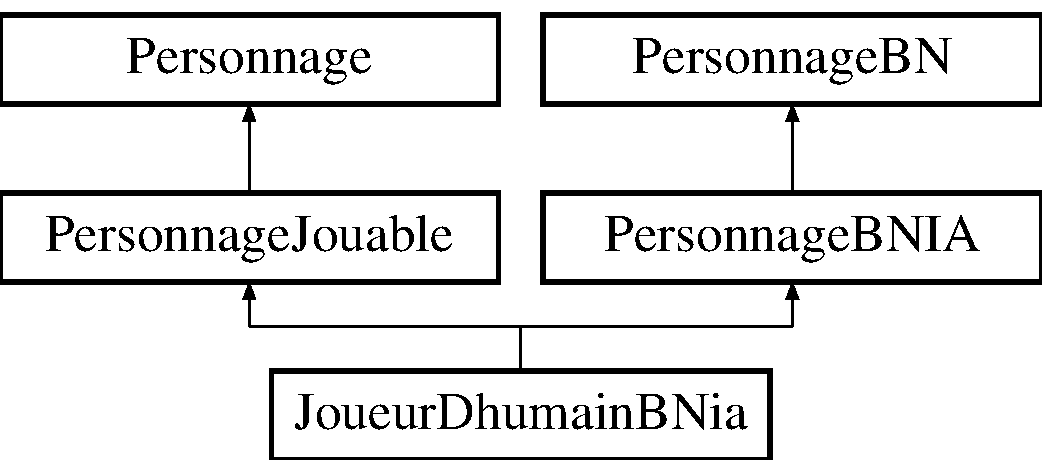
\includegraphics[height=3.000000cm]{classJoueurDhumainBNia}
\end{center}
\end{figure}
\subsection*{Public Member Functions}
\begin{DoxyCompactItemize}
\item 
\hyperlink{classJoueurDhumainBNia_ad730ef7ceffa8698f6fe2c98416f97b5}{Joueur\-Dhumain\-B\-Nia} (string nomnv)
\begin{DoxyCompactList}\small\item\em Constructeur des perso\-B\-N\-I\-A\-Cheate. \end{DoxyCompactList}\item 
\hyperlink{classJoueurDhumainBNia_ab4f8d64413468df76801e2920a37c044}{Joueur\-Dhumain\-B\-Nia} (string nomnv, int l, int h, \hyperlink{classArme}{Arme} $\ast$a)
\begin{DoxyCompactList}\small\item\em Constructeur (très) parametre de personnage\-B\-N\-I\-A\-Cheate. \end{DoxyCompactList}\item 
\hyperlink{classJoueurDhumainBNia_a73b6ae86546a811cc79261f1c0112980}{Joueur\-Dhumain\-B\-Nia} (string nomnv, \hyperlink{classArme}{Arme} $\ast$a)
\begin{DoxyCompactList}\small\item\em Constructeur (très) parametre de personnage\-B\-N\-I\-A\-Cheate. \end{DoxyCompactList}\item 
\hyperlink{classJoueurDhumainBNia_a39fce943bb0edaddb1a91f785e041d57}{Joueur\-Dhumain\-B\-Nia} (string nomnv, int l, int h)
\begin{DoxyCompactList}\small\item\em Constructeur (très) parametre de personnage\-B\-N\-I\-A\-Cheate. \end{DoxyCompactList}\item 
\hyperlink{classJoueurDhumainBNia_acf621e354dcb347a01975bdf9d01af41}{Joueur\-Dhumain\-B\-Nia} (string nomnv, vector$<$ int $>$ t\-Bateaux)
\begin{DoxyCompactList}\small\item\em Constructeur des perso\-B\-N\-I\-A\-Cheate. \end{DoxyCompactList}\item 
\hyperlink{classJoueurDhumainBNia_adb64b580310bb67347ada4ac0462d784}{Joueur\-Dhumain\-B\-Nia} (string nomnv, int l, int h, vector$<$ int $>$ t\-Bateaux, \hyperlink{classArme}{Arme} $\ast$a)
\begin{DoxyCompactList}\small\item\em Constructeur (très) parametre de personnage\-B\-N\-I\-A\-Cheate. \end{DoxyCompactList}\item 
\hyperlink{classJoueurDhumainBNia_a5e05d5a6d274f0c1302cb6452c7c9b76}{Joueur\-Dhumain\-B\-Nia} (string nomnv, vector$<$ int $>$ t\-Bateaux, \hyperlink{classArme}{Arme} $\ast$a)
\begin{DoxyCompactList}\small\item\em Constructeur (très) parametre de personnage\-B\-N\-I\-A\-Cheate. \end{DoxyCompactList}\item 
\hyperlink{classJoueurDhumainBNia_a7c383ccb723c9519d8cf16e1da29492e}{Joueur\-Dhumain\-B\-Nia} (string nomnv, int l, int h, vector$<$ int $>$ t\-Bateaux)
\begin{DoxyCompactList}\small\item\em Constructeur (très) parametre de personnage\-B\-N\-I\-A\-Cheate. \end{DoxyCompactList}\end{DoxyCompactItemize}


\subsection{Detailed Description}
classe définissant un joueur I\-A 

La classe représente un joueur I\-A se déplaçant sur la carte 

\subsection{Constructor \& Destructor Documentation}
\hypertarget{classJoueurDhumainBNia_ad730ef7ceffa8698f6fe2c98416f97b5}{\index{Joueur\-Dhumain\-B\-Nia@{Joueur\-Dhumain\-B\-Nia}!Joueur\-Dhumain\-B\-Nia@{Joueur\-Dhumain\-B\-Nia}}
\index{Joueur\-Dhumain\-B\-Nia@{Joueur\-Dhumain\-B\-Nia}!JoueurDhumainBNia@{Joueur\-Dhumain\-B\-Nia}}
\subsubsection[{Joueur\-Dhumain\-B\-Nia}]{\setlength{\rightskip}{0pt plus 5cm}Joueur\-Dhumain\-B\-Nia\-::\-Joueur\-Dhumain\-B\-Nia (
\begin{DoxyParamCaption}
\item[{string}]{nomnv}
\end{DoxyParamCaption}
)}}\label{classJoueurDhumainBNia_ad730ef7ceffa8698f6fe2c98416f97b5}


Constructeur des perso\-B\-N\-I\-A\-Cheate. 

Constructeur des perso\-B\-N\-I\-A\-Cheate 
\begin{DoxyParams}{Parameters}
{\em nomnv} & \-: nom du joueur \\
\hline
\end{DoxyParams}
\hypertarget{classJoueurDhumainBNia_ab4f8d64413468df76801e2920a37c044}{\index{Joueur\-Dhumain\-B\-Nia@{Joueur\-Dhumain\-B\-Nia}!Joueur\-Dhumain\-B\-Nia@{Joueur\-Dhumain\-B\-Nia}}
\index{Joueur\-Dhumain\-B\-Nia@{Joueur\-Dhumain\-B\-Nia}!JoueurDhumainBNia@{Joueur\-Dhumain\-B\-Nia}}
\subsubsection[{Joueur\-Dhumain\-B\-Nia}]{\setlength{\rightskip}{0pt plus 5cm}Joueur\-Dhumain\-B\-Nia\-::\-Joueur\-Dhumain\-B\-Nia (
\begin{DoxyParamCaption}
\item[{string}]{nomnv, }
\item[{int}]{l, }
\item[{int}]{h, }
\item[{{\bf Arme} $\ast$}]{a}
\end{DoxyParamCaption}
)}}\label{classJoueurDhumainBNia_ab4f8d64413468df76801e2920a37c044}


Constructeur (très) parametre de personnage\-B\-N\-I\-A\-Cheate. 


\begin{DoxyParams}{Parameters}
{\em nomnv} & \-: nom du personnage \\
\hline
{\em l} & \-: longueur de la grille \\
\hline
{\em h} & \-: hauteur de la grille \\
\hline
{\em a} & \-: pointeur sur l'arme souhaitée \\
\hline
\end{DoxyParams}
\hypertarget{classJoueurDhumainBNia_a73b6ae86546a811cc79261f1c0112980}{\index{Joueur\-Dhumain\-B\-Nia@{Joueur\-Dhumain\-B\-Nia}!Joueur\-Dhumain\-B\-Nia@{Joueur\-Dhumain\-B\-Nia}}
\index{Joueur\-Dhumain\-B\-Nia@{Joueur\-Dhumain\-B\-Nia}!JoueurDhumainBNia@{Joueur\-Dhumain\-B\-Nia}}
\subsubsection[{Joueur\-Dhumain\-B\-Nia}]{\setlength{\rightskip}{0pt plus 5cm}Joueur\-Dhumain\-B\-Nia\-::\-Joueur\-Dhumain\-B\-Nia (
\begin{DoxyParamCaption}
\item[{string}]{nomnv, }
\item[{{\bf Arme} $\ast$}]{a}
\end{DoxyParamCaption}
)}}\label{classJoueurDhumainBNia_a73b6ae86546a811cc79261f1c0112980}


Constructeur (très) parametre de personnage\-B\-N\-I\-A\-Cheate. 


\begin{DoxyParams}{Parameters}
{\em nomnv} & \-: nom du personnage \\
\hline
{\em a} & \-: pointeur sur l'arme souhaitée \\
\hline
\end{DoxyParams}
\hypertarget{classJoueurDhumainBNia_a39fce943bb0edaddb1a91f785e041d57}{\index{Joueur\-Dhumain\-B\-Nia@{Joueur\-Dhumain\-B\-Nia}!Joueur\-Dhumain\-B\-Nia@{Joueur\-Dhumain\-B\-Nia}}
\index{Joueur\-Dhumain\-B\-Nia@{Joueur\-Dhumain\-B\-Nia}!JoueurDhumainBNia@{Joueur\-Dhumain\-B\-Nia}}
\subsubsection[{Joueur\-Dhumain\-B\-Nia}]{\setlength{\rightskip}{0pt plus 5cm}Joueur\-Dhumain\-B\-Nia\-::\-Joueur\-Dhumain\-B\-Nia (
\begin{DoxyParamCaption}
\item[{string}]{nomnv, }
\item[{int}]{l, }
\item[{int}]{h}
\end{DoxyParamCaption}
)}}\label{classJoueurDhumainBNia_a39fce943bb0edaddb1a91f785e041d57}


Constructeur (très) parametre de personnage\-B\-N\-I\-A\-Cheate. 


\begin{DoxyParams}{Parameters}
{\em nomnv} & \-: nom du personnage \\
\hline
{\em l} & \-: longueur de la grille \\
\hline
{\em h} & \-: hauteur de la grille \\
\hline
\end{DoxyParams}
\hypertarget{classJoueurDhumainBNia_acf621e354dcb347a01975bdf9d01af41}{\index{Joueur\-Dhumain\-B\-Nia@{Joueur\-Dhumain\-B\-Nia}!Joueur\-Dhumain\-B\-Nia@{Joueur\-Dhumain\-B\-Nia}}
\index{Joueur\-Dhumain\-B\-Nia@{Joueur\-Dhumain\-B\-Nia}!JoueurDhumainBNia@{Joueur\-Dhumain\-B\-Nia}}
\subsubsection[{Joueur\-Dhumain\-B\-Nia}]{\setlength{\rightskip}{0pt plus 5cm}Joueur\-Dhumain\-B\-Nia\-::\-Joueur\-Dhumain\-B\-Nia (
\begin{DoxyParamCaption}
\item[{string}]{nomnv, }
\item[{vector$<$ int $>$}]{t\-Bateaux}
\end{DoxyParamCaption}
)}}\label{classJoueurDhumainBNia_acf621e354dcb347a01975bdf9d01af41}


Constructeur des perso\-B\-N\-I\-A\-Cheate. 

Constructeur des perso\-B\-N\-I\-A\-Cheate 
\begin{DoxyParams}{Parameters}
{\em t\-Bateaux} & \-: vector de taille de bateaux \\
\hline
{\em nomnv} & \-: nom du joueur \\
\hline
\end{DoxyParams}
\hypertarget{classJoueurDhumainBNia_adb64b580310bb67347ada4ac0462d784}{\index{Joueur\-Dhumain\-B\-Nia@{Joueur\-Dhumain\-B\-Nia}!Joueur\-Dhumain\-B\-Nia@{Joueur\-Dhumain\-B\-Nia}}
\index{Joueur\-Dhumain\-B\-Nia@{Joueur\-Dhumain\-B\-Nia}!JoueurDhumainBNia@{Joueur\-Dhumain\-B\-Nia}}
\subsubsection[{Joueur\-Dhumain\-B\-Nia}]{\setlength{\rightskip}{0pt plus 5cm}Joueur\-Dhumain\-B\-Nia\-::\-Joueur\-Dhumain\-B\-Nia (
\begin{DoxyParamCaption}
\item[{string}]{nomnv, }
\item[{int}]{l, }
\item[{int}]{h, }
\item[{vector$<$ int $>$}]{t\-Bateaux, }
\item[{{\bf Arme} $\ast$}]{a}
\end{DoxyParamCaption}
)}}\label{classJoueurDhumainBNia_adb64b580310bb67347ada4ac0462d784}


Constructeur (très) parametre de personnage\-B\-N\-I\-A\-Cheate. 


\begin{DoxyParams}{Parameters}
{\em nomnv} & \-: nom du personnage \\
\hline
{\em t\-Bateaux} & \-: vector de taille de bateaux \\
\hline
{\em l} & \-: longueur de la grille \\
\hline
{\em h} & \-: hauteur de la grille \\
\hline
{\em a} & \-: pointeur sur l'arme souhaitée \\
\hline
\end{DoxyParams}
\hypertarget{classJoueurDhumainBNia_a5e05d5a6d274f0c1302cb6452c7c9b76}{\index{Joueur\-Dhumain\-B\-Nia@{Joueur\-Dhumain\-B\-Nia}!Joueur\-Dhumain\-B\-Nia@{Joueur\-Dhumain\-B\-Nia}}
\index{Joueur\-Dhumain\-B\-Nia@{Joueur\-Dhumain\-B\-Nia}!JoueurDhumainBNia@{Joueur\-Dhumain\-B\-Nia}}
\subsubsection[{Joueur\-Dhumain\-B\-Nia}]{\setlength{\rightskip}{0pt plus 5cm}Joueur\-Dhumain\-B\-Nia\-::\-Joueur\-Dhumain\-B\-Nia (
\begin{DoxyParamCaption}
\item[{string}]{nomnv, }
\item[{vector$<$ int $>$}]{t\-Bateaux, }
\item[{{\bf Arme} $\ast$}]{a}
\end{DoxyParamCaption}
)}}\label{classJoueurDhumainBNia_a5e05d5a6d274f0c1302cb6452c7c9b76}


Constructeur (très) parametre de personnage\-B\-N\-I\-A\-Cheate. 


\begin{DoxyParams}{Parameters}
{\em t\-Bateaux} & \-: vector de taille de bateaux \\
\hline
{\em nomnv} & \-: nom du personnage \\
\hline
{\em a} & \-: pointeur sur l'arme souhaitée \\
\hline
\end{DoxyParams}
\hypertarget{classJoueurDhumainBNia_a7c383ccb723c9519d8cf16e1da29492e}{\index{Joueur\-Dhumain\-B\-Nia@{Joueur\-Dhumain\-B\-Nia}!Joueur\-Dhumain\-B\-Nia@{Joueur\-Dhumain\-B\-Nia}}
\index{Joueur\-Dhumain\-B\-Nia@{Joueur\-Dhumain\-B\-Nia}!JoueurDhumainBNia@{Joueur\-Dhumain\-B\-Nia}}
\subsubsection[{Joueur\-Dhumain\-B\-Nia}]{\setlength{\rightskip}{0pt plus 5cm}Joueur\-Dhumain\-B\-Nia\-::\-Joueur\-Dhumain\-B\-Nia (
\begin{DoxyParamCaption}
\item[{string}]{nomnv, }
\item[{int}]{l, }
\item[{int}]{h, }
\item[{vector$<$ int $>$}]{t\-Bateaux}
\end{DoxyParamCaption}
)}}\label{classJoueurDhumainBNia_a7c383ccb723c9519d8cf16e1da29492e}


Constructeur (très) parametre de personnage\-B\-N\-I\-A\-Cheate. 


\begin{DoxyParams}{Parameters}
{\em nomnv} & \-: nom du personnage \\
\hline
{\em t\-Bateaux} & \-: vector de taille de bateaux \\
\hline
{\em l} & \-: longueur de la grille \\
\hline
{\em h} & \-: hauteur de la grille \\
\hline
\end{DoxyParams}


The documentation for this class was generated from the following files\-:\begin{DoxyCompactItemize}
\item 
/home/damien/\-Bureau/projetcpp\-\_\-gm42/source/src/\hyperlink{JoueurDhumainBNia_8hpp}{Joueur\-Dhumain\-B\-Nia.\-hpp}\item 
/home/damien/\-Bureau/projetcpp\-\_\-gm42/source/src/Joueur\-Dhumain\-B\-Nia.\-cpp\end{DoxyCompactItemize}

\hypertarget{classJoueurHumain}{\section{Joueur\-Humain Class Reference}
\label{classJoueurHumain}\index{Joueur\-Humain@{Joueur\-Humain}}
}


classe définissant un joueur humain  




{\ttfamily \#include $<$Joueur\-Humain.\-hpp$>$}

Inheritance diagram for Joueur\-Humain\-:\begin{figure}[H]
\begin{center}
\leavevmode
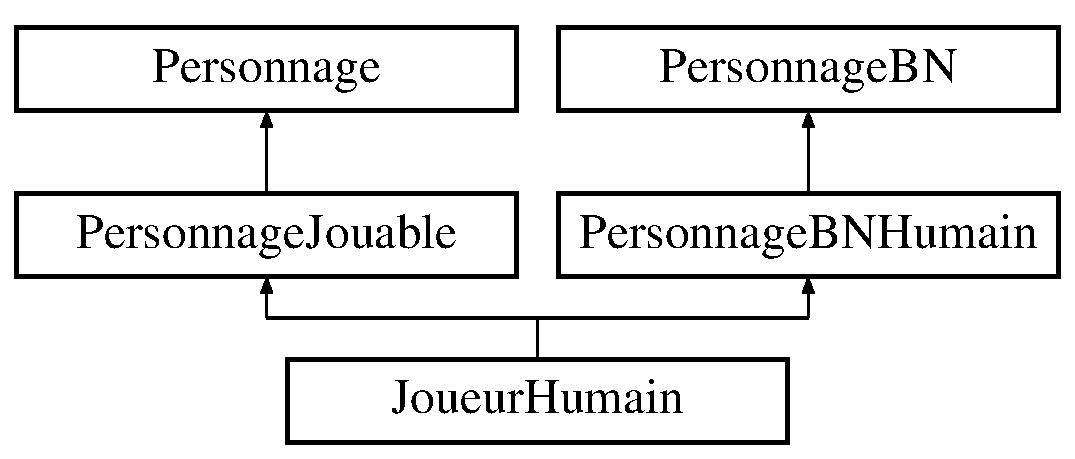
\includegraphics[height=3.000000cm]{classJoueurHumain}
\end{center}
\end{figure}
\subsection*{Public Member Functions}
\begin{DoxyCompactItemize}
\item 
\hyperlink{classJoueurHumain_a28fc9a25bbd04a3126940898e7caa068}{Joueur\-Humain} (string nomnv, \hyperlink{classCoordonnees}{Coordonnees} coord, \hyperlink{classCarte}{Carte} $\ast$id\-Carte)
\begin{DoxyCompactList}\small\item\em Constructeur des perso\-B\-N\-I\-A\-Cheate. \end{DoxyCompactList}\item 
\hyperlink{classJoueurHumain_a6c7cda10e16fcfdfa613fe069b005d29}{Joueur\-Humain} (string nomnv, int l, int h, \hyperlink{classArme}{Arme} $\ast$a, \hyperlink{classCoordonnees}{Coordonnees} coord, \hyperlink{classCarte}{Carte} $\ast$id\-Carte)
\begin{DoxyCompactList}\small\item\em Constructeur (très) parametre de personnage\-B\-N\-I\-A\-Cheate. \end{DoxyCompactList}\item 
\hyperlink{classJoueurHumain_a2dbf1390b2f6d45377fdd40eaea6c9c3}{Joueur\-Humain} (string nomnv, \hyperlink{classArme}{Arme} $\ast$a, \hyperlink{classCoordonnees}{Coordonnees} coord, \hyperlink{classCarte}{Carte} $\ast$id\-Carte)
\begin{DoxyCompactList}\small\item\em Constructeur (très) parametre de personnage\-B\-N\-I\-A\-Cheate. \end{DoxyCompactList}\item 
\hyperlink{classJoueurHumain_adc6ce23d4235296e6ff795ec0d7a7f34}{Joueur\-Humain} (string nomnv, int l, int h, \hyperlink{classCoordonnees}{Coordonnees} coord, \hyperlink{classCarte}{Carte} $\ast$id\-Carte)
\begin{DoxyCompactList}\small\item\em Constructeur (très) parametre de personnage\-B\-N\-I\-A\-Cheate. \end{DoxyCompactList}\item 
\hyperlink{classJoueurHumain_a48879a6505888acf397787792ea3a2fb}{Joueur\-Humain} (string nomnv, vector$<$ int $>$ t\-Bateaux, \hyperlink{classCoordonnees}{Coordonnees} coord, \hyperlink{classCarte}{Carte} $\ast$id\-Carte)
\begin{DoxyCompactList}\small\item\em Constructeur des perso\-B\-N\-I\-A\-Cheate. \end{DoxyCompactList}\item 
\hyperlink{classJoueurHumain_af8eb95136a3d0be7a0a78784001cd8d1}{Joueur\-Humain} (string nomnv, int l, int h, vector$<$ int $>$ t\-Bateaux, \hyperlink{classArme}{Arme} $\ast$a, \hyperlink{classCoordonnees}{Coordonnees} coord, \hyperlink{classCarte}{Carte} $\ast$id\-Carte)
\begin{DoxyCompactList}\small\item\em Constructeur (très) parametre de personnage\-B\-N\-I\-A\-Cheate. \end{DoxyCompactList}\item 
\hyperlink{classJoueurHumain_a0a7411206a3cf4225ecb1a5fcd3cdabd}{Joueur\-Humain} (string nomnv, vector$<$ int $>$ t\-Bateaux, \hyperlink{classArme}{Arme} $\ast$a, \hyperlink{classCoordonnees}{Coordonnees} coord, \hyperlink{classCarte}{Carte} $\ast$id\-Carte)
\begin{DoxyCompactList}\small\item\em Constructeur (très) parametre de personnage\-B\-N\-I\-A\-Cheate. \end{DoxyCompactList}\item 
\hyperlink{classJoueurHumain_af963014be7f32bad0b40745e726d0a39}{Joueur\-Humain} (string nomnv, int l, int h, vector$<$ int $>$ t\-Bateaux, \hyperlink{classCoordonnees}{Coordonnees} coord, \hyperlink{classCarte}{Carte} $\ast$id\-Carte)
\begin{DoxyCompactList}\small\item\em Constructeur (très) parametre de personnage\-B\-N\-I\-A\-Cheate. \end{DoxyCompactList}\end{DoxyCompactItemize}


\subsection{Detailed Description}
classe définissant un joueur humain 

La classe représente un joueur humain se déplaçant sur la carte 

\subsection{Constructor \& Destructor Documentation}
\hypertarget{classJoueurHumain_a28fc9a25bbd04a3126940898e7caa068}{\index{Joueur\-Humain@{Joueur\-Humain}!Joueur\-Humain@{Joueur\-Humain}}
\index{Joueur\-Humain@{Joueur\-Humain}!JoueurHumain@{Joueur\-Humain}}
\subsubsection[{Joueur\-Humain}]{\setlength{\rightskip}{0pt plus 5cm}Joueur\-Humain\-::\-Joueur\-Humain (
\begin{DoxyParamCaption}
\item[{string}]{nomnv, }
\item[{{\bf Coordonnees}}]{coord, }
\item[{{\bf Carte} $\ast$}]{id\-Carte}
\end{DoxyParamCaption}
)}}\label{classJoueurHumain_a28fc9a25bbd04a3126940898e7caa068}


Constructeur des perso\-B\-N\-I\-A\-Cheate. 

Constructeur des perso\-B\-N\-I\-A\-Cheate 
\begin{DoxyParams}{Parameters}
{\em nomnv} & \-: nom du joueur \\
\hline
{\em coord} & \-: coordonnees initiale du personnage \\
\hline
{\em id\-Carte} & \-: carte initiale du personnage \\
\hline
\end{DoxyParams}
\hypertarget{classJoueurHumain_a6c7cda10e16fcfdfa613fe069b005d29}{\index{Joueur\-Humain@{Joueur\-Humain}!Joueur\-Humain@{Joueur\-Humain}}
\index{Joueur\-Humain@{Joueur\-Humain}!JoueurHumain@{Joueur\-Humain}}
\subsubsection[{Joueur\-Humain}]{\setlength{\rightskip}{0pt plus 5cm}Joueur\-Humain\-::\-Joueur\-Humain (
\begin{DoxyParamCaption}
\item[{string}]{nomnv, }
\item[{int}]{l, }
\item[{int}]{h, }
\item[{{\bf Arme} $\ast$}]{a, }
\item[{{\bf Coordonnees}}]{coord, }
\item[{{\bf Carte} $\ast$}]{id\-Carte}
\end{DoxyParamCaption}
)}}\label{classJoueurHumain_a6c7cda10e16fcfdfa613fe069b005d29}


Constructeur (très) parametre de personnage\-B\-N\-I\-A\-Cheate. 


\begin{DoxyParams}{Parameters}
{\em nomnv} & \-: nom du personnage \\
\hline
{\em l} & \-: longueur de la grille \\
\hline
{\em h} & \-: hauteur de la grille \\
\hline
{\em a} & \-: pointeur sur l'arme souhaitée \\
\hline
{\em coord} & \-: coordonnees initiale du personnage \\
\hline
{\em id\-Carte} & \-: carte initiale du personnage \\
\hline
\end{DoxyParams}
\hypertarget{classJoueurHumain_a2dbf1390b2f6d45377fdd40eaea6c9c3}{\index{Joueur\-Humain@{Joueur\-Humain}!Joueur\-Humain@{Joueur\-Humain}}
\index{Joueur\-Humain@{Joueur\-Humain}!JoueurHumain@{Joueur\-Humain}}
\subsubsection[{Joueur\-Humain}]{\setlength{\rightskip}{0pt plus 5cm}Joueur\-Humain\-::\-Joueur\-Humain (
\begin{DoxyParamCaption}
\item[{string}]{nomnv, }
\item[{{\bf Arme} $\ast$}]{a, }
\item[{{\bf Coordonnees}}]{coord, }
\item[{{\bf Carte} $\ast$}]{id\-Carte}
\end{DoxyParamCaption}
)}}\label{classJoueurHumain_a2dbf1390b2f6d45377fdd40eaea6c9c3}


Constructeur (très) parametre de personnage\-B\-N\-I\-A\-Cheate. 


\begin{DoxyParams}{Parameters}
{\em nomnv} & \-: nom du personnage \\
\hline
{\em a} & \-: pointeur sur l'arme souhaitée \\
\hline
{\em coord} & \-: coordonnees initiale du personnage \\
\hline
{\em id\-Carte} & \-: carte initiale du personnage \\
\hline
\end{DoxyParams}
\hypertarget{classJoueurHumain_adc6ce23d4235296e6ff795ec0d7a7f34}{\index{Joueur\-Humain@{Joueur\-Humain}!Joueur\-Humain@{Joueur\-Humain}}
\index{Joueur\-Humain@{Joueur\-Humain}!JoueurHumain@{Joueur\-Humain}}
\subsubsection[{Joueur\-Humain}]{\setlength{\rightskip}{0pt plus 5cm}Joueur\-Humain\-::\-Joueur\-Humain (
\begin{DoxyParamCaption}
\item[{string}]{nomnv, }
\item[{int}]{l, }
\item[{int}]{h, }
\item[{{\bf Coordonnees}}]{coord, }
\item[{{\bf Carte} $\ast$}]{id\-Carte}
\end{DoxyParamCaption}
)}}\label{classJoueurHumain_adc6ce23d4235296e6ff795ec0d7a7f34}


Constructeur (très) parametre de personnage\-B\-N\-I\-A\-Cheate. 


\begin{DoxyParams}{Parameters}
{\em nomnv} & \-: nom du personnage \\
\hline
{\em l} & \-: longueur de la grille \\
\hline
{\em h} & \-: hauteur de la grille \\
\hline
{\em coord} & \-: coordonnees initiale du personnage \\
\hline
{\em id\-Carte} & \-: carte initiale du personnage \\
\hline
\end{DoxyParams}
\hypertarget{classJoueurHumain_a48879a6505888acf397787792ea3a2fb}{\index{Joueur\-Humain@{Joueur\-Humain}!Joueur\-Humain@{Joueur\-Humain}}
\index{Joueur\-Humain@{Joueur\-Humain}!JoueurHumain@{Joueur\-Humain}}
\subsubsection[{Joueur\-Humain}]{\setlength{\rightskip}{0pt plus 5cm}Joueur\-Humain\-::\-Joueur\-Humain (
\begin{DoxyParamCaption}
\item[{string}]{nomnv, }
\item[{vector$<$ int $>$}]{t\-Bateaux, }
\item[{{\bf Coordonnees}}]{coord, }
\item[{{\bf Carte} $\ast$}]{id\-Carte}
\end{DoxyParamCaption}
)}}\label{classJoueurHumain_a48879a6505888acf397787792ea3a2fb}


Constructeur des perso\-B\-N\-I\-A\-Cheate. 

Constructeur des perso\-B\-N\-I\-A\-Cheate 
\begin{DoxyParams}{Parameters}
{\em t\-Bateaux} & \-: vector de taille de bateaux \\
\hline
{\em nomnv} & \-: nom du joueur \\
\hline
{\em coord} & \-: coordonnees initiale du personnage \\
\hline
{\em id\-Carte} & \-: carte initiale du personnage \\
\hline
\end{DoxyParams}
\hypertarget{classJoueurHumain_af8eb95136a3d0be7a0a78784001cd8d1}{\index{Joueur\-Humain@{Joueur\-Humain}!Joueur\-Humain@{Joueur\-Humain}}
\index{Joueur\-Humain@{Joueur\-Humain}!JoueurHumain@{Joueur\-Humain}}
\subsubsection[{Joueur\-Humain}]{\setlength{\rightskip}{0pt plus 5cm}Joueur\-Humain\-::\-Joueur\-Humain (
\begin{DoxyParamCaption}
\item[{string}]{nomnv, }
\item[{int}]{l, }
\item[{int}]{h, }
\item[{vector$<$ int $>$}]{t\-Bateaux, }
\item[{{\bf Arme} $\ast$}]{a, }
\item[{{\bf Coordonnees}}]{coord, }
\item[{{\bf Carte} $\ast$}]{id\-Carte}
\end{DoxyParamCaption}
)}}\label{classJoueurHumain_af8eb95136a3d0be7a0a78784001cd8d1}


Constructeur (très) parametre de personnage\-B\-N\-I\-A\-Cheate. 


\begin{DoxyParams}{Parameters}
{\em nomnv} & \-: nom du personnage \\
\hline
{\em t\-Bateaux} & \-: vector de taille de bateaux \\
\hline
{\em l} & \-: longueur de la grille \\
\hline
{\em h} & \-: hauteur de la grille \\
\hline
{\em a} & \-: pointeur sur l'arme souhaitée \\
\hline
{\em coord} & \-: coordonnees initiale du personnage \\
\hline
{\em id\-Carte} & \-: carte initiale du personnage \\
\hline
\end{DoxyParams}
\hypertarget{classJoueurHumain_a0a7411206a3cf4225ecb1a5fcd3cdabd}{\index{Joueur\-Humain@{Joueur\-Humain}!Joueur\-Humain@{Joueur\-Humain}}
\index{Joueur\-Humain@{Joueur\-Humain}!JoueurHumain@{Joueur\-Humain}}
\subsubsection[{Joueur\-Humain}]{\setlength{\rightskip}{0pt plus 5cm}Joueur\-Humain\-::\-Joueur\-Humain (
\begin{DoxyParamCaption}
\item[{string}]{nomnv, }
\item[{vector$<$ int $>$}]{t\-Bateaux, }
\item[{{\bf Arme} $\ast$}]{a, }
\item[{{\bf Coordonnees}}]{coord, }
\item[{{\bf Carte} $\ast$}]{id\-Carte}
\end{DoxyParamCaption}
)}}\label{classJoueurHumain_a0a7411206a3cf4225ecb1a5fcd3cdabd}


Constructeur (très) parametre de personnage\-B\-N\-I\-A\-Cheate. 


\begin{DoxyParams}{Parameters}
{\em t\-Bateaux} & \-: vector de taille de bateaux \\
\hline
{\em nomnv} & \-: nom du personnage \\
\hline
{\em a} & \-: pointeur sur l'arme souhaitée \\
\hline
{\em coord} & \-: coordonnees initiale du personnage \\
\hline
{\em id\-Carte} & \-: carte initiale du personnage \\
\hline
\end{DoxyParams}
\hypertarget{classJoueurHumain_af963014be7f32bad0b40745e726d0a39}{\index{Joueur\-Humain@{Joueur\-Humain}!Joueur\-Humain@{Joueur\-Humain}}
\index{Joueur\-Humain@{Joueur\-Humain}!JoueurHumain@{Joueur\-Humain}}
\subsubsection[{Joueur\-Humain}]{\setlength{\rightskip}{0pt plus 5cm}Joueur\-Humain\-::\-Joueur\-Humain (
\begin{DoxyParamCaption}
\item[{string}]{nomnv, }
\item[{int}]{l, }
\item[{int}]{h, }
\item[{vector$<$ int $>$}]{t\-Bateaux, }
\item[{{\bf Coordonnees}}]{coord, }
\item[{{\bf Carte} $\ast$}]{id\-Carte}
\end{DoxyParamCaption}
)}}\label{classJoueurHumain_af963014be7f32bad0b40745e726d0a39}


Constructeur (très) parametre de personnage\-B\-N\-I\-A\-Cheate. 


\begin{DoxyParams}{Parameters}
{\em nomnv} & \-: nom du personnage \\
\hline
{\em t\-Bateaux} & \-: vector de taille de bateaux \\
\hline
{\em l} & \-: longueur de la grille \\
\hline
{\em h} & \-: hauteur de la grille \\
\hline
{\em coord} & \-: coordonnees initiale du personnage \\
\hline
{\em id\-Carte} & \-: carte initiale du personnage \\
\hline
\end{DoxyParams}


The documentation for this class was generated from the following files\-:\begin{DoxyCompactItemize}
\item 
/home/damien/\-Bureau/projetcpp\-\_\-gm42/source/src/\hyperlink{JoueurHumain_8hpp}{Joueur\-Humain.\-hpp}\item 
/home/damien/\-Bureau/projetcpp\-\_\-gm42/source/src/Joueur\-Humain.\-cpp\end{DoxyCompactItemize}

\hypertarget{classJoueurIA}{\section{Joueur\-I\-A Class Reference}
\label{classJoueurIA}\index{Joueur\-I\-A@{Joueur\-I\-A}}
}


classe définissant un joueur I\-A  




{\ttfamily \#include $<$Joueur\-I\-A.\-hpp$>$}

Inheritance diagram for Joueur\-I\-A\-:\begin{figure}[H]
\begin{center}
\leavevmode
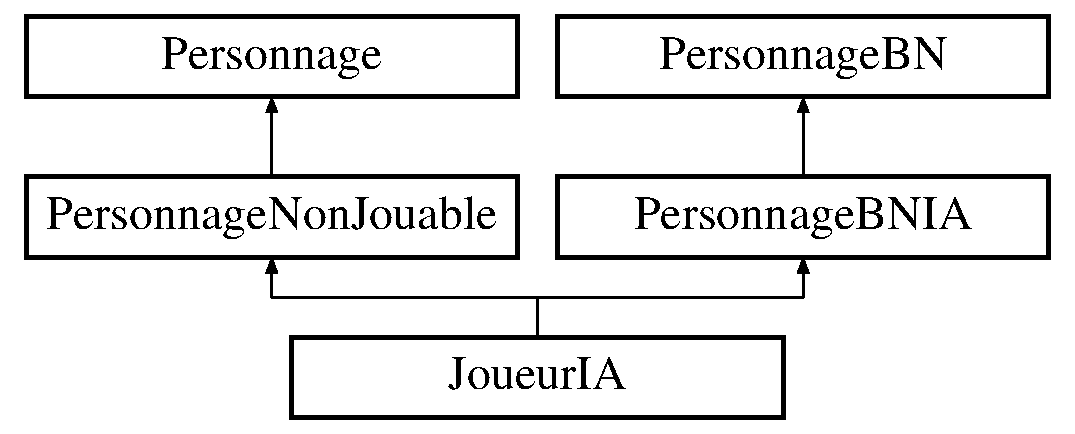
\includegraphics[height=3.000000cm]{classJoueurIA}
\end{center}
\end{figure}
\subsection*{Public Member Functions}
\begin{DoxyCompactItemize}
\item 
\hyperlink{classJoueurIA_a95ee959f123d5edc3aa4ec00a0419b0d}{Joueur\-I\-A} (string nomnv)
\begin{DoxyCompactList}\small\item\em Constructeur des perso\-B\-N\-I\-A. \end{DoxyCompactList}\item 
\hyperlink{classJoueurIA_a2ade22afbf5d6a16f31c19c2854b89d8}{Joueur\-I\-A} (string nomnv, int l, int h, \hyperlink{classArme}{Arme} $\ast$a)
\begin{DoxyCompactList}\small\item\em Constructeur (très) parametre de personnage\-B\-N\-I\-A. \end{DoxyCompactList}\item 
\hyperlink{classJoueurIA_a2ce9a7329cac275748d069c68b81b042}{Joueur\-I\-A} (string nomnv, \hyperlink{classArme}{Arme} $\ast$a)
\begin{DoxyCompactList}\small\item\em Constructeur (très) parametre de personnage\-B\-N\-I\-A. \end{DoxyCompactList}\item 
\hyperlink{classJoueurIA_acd72db6b7768b7ae7edfba843f0b5ea9}{Joueur\-I\-A} (string nomnv, int l, int h)
\begin{DoxyCompactList}\small\item\em Constructeur (très) parametre de personnage\-B\-N\-I\-A. \end{DoxyCompactList}\item 
\hyperlink{classJoueurIA_a169acc5a53a751f182ff4605d63a8f20}{Joueur\-I\-A} (string nomnv, vector$<$ int $>$ t\-Bateaux)
\begin{DoxyCompactList}\small\item\em Constructeur des perso\-B\-N\-I\-A. \end{DoxyCompactList}\item 
\hyperlink{classJoueurIA_a6524d958b7e2739f7758be25bbf721d5}{Joueur\-I\-A} (string nomnv, int l, int h, vector$<$ int $>$ t\-Bateaux, \hyperlink{classArme}{Arme} $\ast$a)
\begin{DoxyCompactList}\small\item\em Constructeur (très) parametre de personnage\-B\-N\-I\-A. \end{DoxyCompactList}\item 
\hyperlink{classJoueurIA_a74ede3529c5f3d9c6b081d5c34a57ae5}{Joueur\-I\-A} (string nomnv, vector$<$ int $>$ t\-Bateaux, \hyperlink{classArme}{Arme} $\ast$a)
\begin{DoxyCompactList}\small\item\em Constructeur (très) parametre de personnage\-B\-N\-I\-A. \end{DoxyCompactList}\item 
\hyperlink{classJoueurIA_a9ef8471f45f438b4474e6ed6facee3d8}{Joueur\-I\-A} (string nomnv, int l, int h, vector$<$ int $>$ t\-Bateaux)
\begin{DoxyCompactList}\small\item\em Constructeur (très) parametre de personnage\-B\-N\-I\-A. \end{DoxyCompactList}\end{DoxyCompactItemize}


\subsection{Detailed Description}
classe définissant un joueur I\-A 

La classe représente un joueur I\-A se déplaçant sur la carte 

\subsection{Constructor \& Destructor Documentation}
\hypertarget{classJoueurIA_a95ee959f123d5edc3aa4ec00a0419b0d}{\index{Joueur\-I\-A@{Joueur\-I\-A}!Joueur\-I\-A@{Joueur\-I\-A}}
\index{Joueur\-I\-A@{Joueur\-I\-A}!JoueurIA@{Joueur\-I\-A}}
\subsubsection[{Joueur\-I\-A}]{\setlength{\rightskip}{0pt plus 5cm}Joueur\-I\-A\-::\-Joueur\-I\-A (
\begin{DoxyParamCaption}
\item[{string}]{nomnv}
\end{DoxyParamCaption}
)}}\label{classJoueurIA_a95ee959f123d5edc3aa4ec00a0419b0d}


Constructeur des perso\-B\-N\-I\-A. 

Constructeur des perso\-B\-N\-I\-A 
\begin{DoxyParams}{Parameters}
{\em nomnv} & \-: nom du joueur \\
\hline
\end{DoxyParams}
\hypertarget{classJoueurIA_a2ade22afbf5d6a16f31c19c2854b89d8}{\index{Joueur\-I\-A@{Joueur\-I\-A}!Joueur\-I\-A@{Joueur\-I\-A}}
\index{Joueur\-I\-A@{Joueur\-I\-A}!JoueurIA@{Joueur\-I\-A}}
\subsubsection[{Joueur\-I\-A}]{\setlength{\rightskip}{0pt plus 5cm}Joueur\-I\-A\-::\-Joueur\-I\-A (
\begin{DoxyParamCaption}
\item[{string}]{nomnv, }
\item[{int}]{l, }
\item[{int}]{h, }
\item[{{\bf Arme} $\ast$}]{a}
\end{DoxyParamCaption}
)}}\label{classJoueurIA_a2ade22afbf5d6a16f31c19c2854b89d8}


Constructeur (très) parametre de personnage\-B\-N\-I\-A. 


\begin{DoxyParams}{Parameters}
{\em nomnv} & \-: nom du personnage \\
\hline
{\em l} & \-: longueur de la grille \\
\hline
{\em h} & \-: hauteur de la grille \\
\hline
{\em a} & \-: pointeur sur l'arme souhaitée \\
\hline
\end{DoxyParams}
\hypertarget{classJoueurIA_a2ce9a7329cac275748d069c68b81b042}{\index{Joueur\-I\-A@{Joueur\-I\-A}!Joueur\-I\-A@{Joueur\-I\-A}}
\index{Joueur\-I\-A@{Joueur\-I\-A}!JoueurIA@{Joueur\-I\-A}}
\subsubsection[{Joueur\-I\-A}]{\setlength{\rightskip}{0pt plus 5cm}Joueur\-I\-A\-::\-Joueur\-I\-A (
\begin{DoxyParamCaption}
\item[{string}]{nomnv, }
\item[{{\bf Arme} $\ast$}]{a}
\end{DoxyParamCaption}
)}}\label{classJoueurIA_a2ce9a7329cac275748d069c68b81b042}


Constructeur (très) parametre de personnage\-B\-N\-I\-A. 


\begin{DoxyParams}{Parameters}
{\em nomnv} & \-: nom du personnage \\
\hline
{\em a} & \-: pointeur sur l'arme souhaitée \\
\hline
\end{DoxyParams}
\hypertarget{classJoueurIA_acd72db6b7768b7ae7edfba843f0b5ea9}{\index{Joueur\-I\-A@{Joueur\-I\-A}!Joueur\-I\-A@{Joueur\-I\-A}}
\index{Joueur\-I\-A@{Joueur\-I\-A}!JoueurIA@{Joueur\-I\-A}}
\subsubsection[{Joueur\-I\-A}]{\setlength{\rightskip}{0pt plus 5cm}Joueur\-I\-A\-::\-Joueur\-I\-A (
\begin{DoxyParamCaption}
\item[{string}]{nomnv, }
\item[{int}]{l, }
\item[{int}]{h}
\end{DoxyParamCaption}
)}}\label{classJoueurIA_acd72db6b7768b7ae7edfba843f0b5ea9}


Constructeur (très) parametre de personnage\-B\-N\-I\-A. 


\begin{DoxyParams}{Parameters}
{\em nomnv} & \-: nom du personnage \\
\hline
{\em l} & \-: longueur de la grille \\
\hline
{\em h} & \-: hauteur de la grille \\
\hline
\end{DoxyParams}
\hypertarget{classJoueurIA_a169acc5a53a751f182ff4605d63a8f20}{\index{Joueur\-I\-A@{Joueur\-I\-A}!Joueur\-I\-A@{Joueur\-I\-A}}
\index{Joueur\-I\-A@{Joueur\-I\-A}!JoueurIA@{Joueur\-I\-A}}
\subsubsection[{Joueur\-I\-A}]{\setlength{\rightskip}{0pt plus 5cm}Joueur\-I\-A\-::\-Joueur\-I\-A (
\begin{DoxyParamCaption}
\item[{string}]{nomnv, }
\item[{vector$<$ int $>$}]{t\-Bateaux}
\end{DoxyParamCaption}
)}}\label{classJoueurIA_a169acc5a53a751f182ff4605d63a8f20}


Constructeur des perso\-B\-N\-I\-A. 

Constructeur des perso\-B\-N\-I\-A 
\begin{DoxyParams}{Parameters}
{\em t\-Bateaux} & \-: vector de taille de bateaux \\
\hline
{\em nomnv} & \-: nom du joueur \\
\hline
\end{DoxyParams}
\hypertarget{classJoueurIA_a6524d958b7e2739f7758be25bbf721d5}{\index{Joueur\-I\-A@{Joueur\-I\-A}!Joueur\-I\-A@{Joueur\-I\-A}}
\index{Joueur\-I\-A@{Joueur\-I\-A}!JoueurIA@{Joueur\-I\-A}}
\subsubsection[{Joueur\-I\-A}]{\setlength{\rightskip}{0pt plus 5cm}Joueur\-I\-A\-::\-Joueur\-I\-A (
\begin{DoxyParamCaption}
\item[{string}]{nomnv, }
\item[{int}]{l, }
\item[{int}]{h, }
\item[{vector$<$ int $>$}]{t\-Bateaux, }
\item[{{\bf Arme} $\ast$}]{a}
\end{DoxyParamCaption}
)}}\label{classJoueurIA_a6524d958b7e2739f7758be25bbf721d5}


Constructeur (très) parametre de personnage\-B\-N\-I\-A. 


\begin{DoxyParams}{Parameters}
{\em nomnv} & \-: nom du personnage \\
\hline
{\em t\-Bateaux} & \-: vector de taille de bateaux \\
\hline
{\em l} & \-: longueur de la grille \\
\hline
{\em h} & \-: hauteur de la grille \\
\hline
{\em a} & \-: pointeur sur l'arme souhaitée \\
\hline
\end{DoxyParams}
\hypertarget{classJoueurIA_a74ede3529c5f3d9c6b081d5c34a57ae5}{\index{Joueur\-I\-A@{Joueur\-I\-A}!Joueur\-I\-A@{Joueur\-I\-A}}
\index{Joueur\-I\-A@{Joueur\-I\-A}!JoueurIA@{Joueur\-I\-A}}
\subsubsection[{Joueur\-I\-A}]{\setlength{\rightskip}{0pt plus 5cm}Joueur\-I\-A\-::\-Joueur\-I\-A (
\begin{DoxyParamCaption}
\item[{string}]{nomnv, }
\item[{vector$<$ int $>$}]{t\-Bateaux, }
\item[{{\bf Arme} $\ast$}]{a}
\end{DoxyParamCaption}
)}}\label{classJoueurIA_a74ede3529c5f3d9c6b081d5c34a57ae5}


Constructeur (très) parametre de personnage\-B\-N\-I\-A. 


\begin{DoxyParams}{Parameters}
{\em t\-Bateaux} & \-: vector de taille de bateaux \\
\hline
{\em nomnv} & \-: nom du personnage \\
\hline
{\em a} & \-: pointeur sur l'arme souhaitée \\
\hline
\end{DoxyParams}
\hypertarget{classJoueurIA_a9ef8471f45f438b4474e6ed6facee3d8}{\index{Joueur\-I\-A@{Joueur\-I\-A}!Joueur\-I\-A@{Joueur\-I\-A}}
\index{Joueur\-I\-A@{Joueur\-I\-A}!JoueurIA@{Joueur\-I\-A}}
\subsubsection[{Joueur\-I\-A}]{\setlength{\rightskip}{0pt plus 5cm}Joueur\-I\-A\-::\-Joueur\-I\-A (
\begin{DoxyParamCaption}
\item[{string}]{nomnv, }
\item[{int}]{l, }
\item[{int}]{h, }
\item[{vector$<$ int $>$}]{t\-Bateaux}
\end{DoxyParamCaption}
)}}\label{classJoueurIA_a9ef8471f45f438b4474e6ed6facee3d8}


Constructeur (très) parametre de personnage\-B\-N\-I\-A. 


\begin{DoxyParams}{Parameters}
{\em nomnv} & \-: nom du personnage \\
\hline
{\em t\-Bateaux} & \-: vector de taille de bateaux \\
\hline
{\em l} & \-: longueur de la grille \\
\hline
{\em h} & \-: hauteur de la grille \\
\hline
\end{DoxyParams}


The documentation for this class was generated from the following files\-:\begin{DoxyCompactItemize}
\item 
/home/damien/\-Bureau/projetcpp\-\_\-gm42/source/src/\hyperlink{JoueurIA_8hpp}{Joueur\-I\-A.\-hpp}\item 
/home/damien/\-Bureau/projetcpp\-\_\-gm42/source/src/Joueur\-I\-A.\-cpp\end{DoxyCompactItemize}

\hypertarget{classJoueurIAAvance}{\section{Joueur\-I\-A\-Avance Class Reference}
\label{classJoueurIAAvance}\index{Joueur\-I\-A\-Avance@{Joueur\-I\-A\-Avance}}
}


classe définissant un joueur I\-A  




{\ttfamily \#include $<$Joueur\-I\-A\-Avance.\-hpp$>$}

Inheritance diagram for Joueur\-I\-A\-Avance\-:\begin{figure}[H]
\begin{center}
\leavevmode
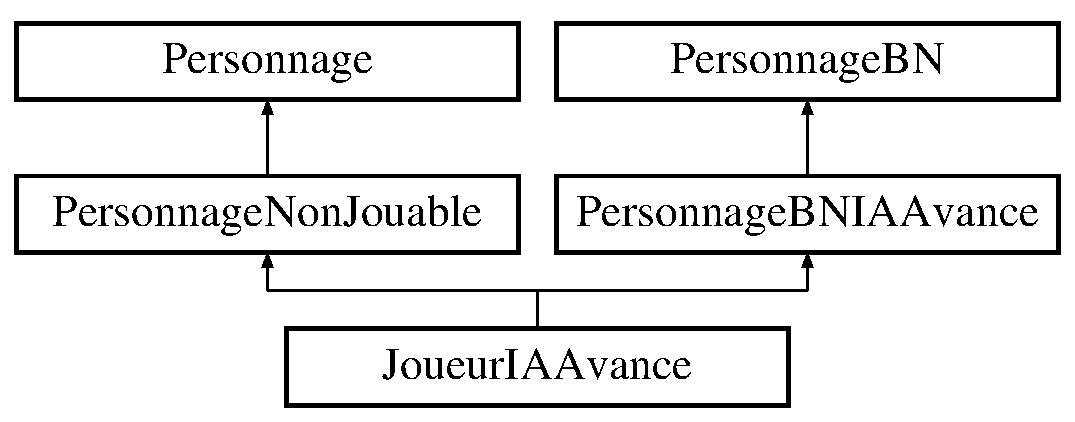
\includegraphics[height=3.000000cm]{classJoueurIAAvance}
\end{center}
\end{figure}
\subsection*{Public Member Functions}
\begin{DoxyCompactItemize}
\item 
\hyperlink{classJoueurIAAvance_afd35289c0c99c9907aa74f7951d6d493}{Joueur\-I\-A\-Avance} (string nomnv)
\begin{DoxyCompactList}\small\item\em Constructeur des perso\-B\-N\-I\-A\-Cheate. \end{DoxyCompactList}\item 
\hyperlink{classJoueurIAAvance_aa4a13dd7828d55388cb3aa3c6f37d19a}{Joueur\-I\-A\-Avance} (string nomnv, int l, int h, \hyperlink{classArme}{Arme} $\ast$a)
\begin{DoxyCompactList}\small\item\em Constructeur (très) parametre de personnage\-B\-N\-I\-A\-Cheate. \end{DoxyCompactList}\item 
\hyperlink{classJoueurIAAvance_a300ba264da26073b86421fa56aaf2480}{Joueur\-I\-A\-Avance} (string nomnv, \hyperlink{classArme}{Arme} $\ast$a)
\begin{DoxyCompactList}\small\item\em Constructeur (très) parametre de personnage\-B\-N\-I\-A\-Cheate. \end{DoxyCompactList}\item 
\hyperlink{classJoueurIAAvance_a6f98205a559a9a7534e4cec8f3ad1235}{Joueur\-I\-A\-Avance} (string nomnv, int l, int h)
\begin{DoxyCompactList}\small\item\em Constructeur (très) parametre de personnage\-B\-N\-I\-A\-Cheate. \end{DoxyCompactList}\item 
\hyperlink{classJoueurIAAvance_ae42874056d41e9be7952bfc279739a88}{Joueur\-I\-A\-Avance} (string nomnv, vector$<$ int $>$ t\-Bateaux)
\begin{DoxyCompactList}\small\item\em Constructeur des perso\-B\-N\-I\-A\-Cheate. \end{DoxyCompactList}\item 
\hyperlink{classJoueurIAAvance_afd25e5803822139fb16a4a003cdabfa0}{Joueur\-I\-A\-Avance} (string nomnv, int l, int h, vector$<$ int $>$ t\-Bateaux, \hyperlink{classArme}{Arme} $\ast$a)
\begin{DoxyCompactList}\small\item\em Constructeur (très) parametre de personnage\-B\-N\-I\-A\-Cheate. \end{DoxyCompactList}\item 
\hyperlink{classJoueurIAAvance_a70dd9cffdf35743d1021f5010dadd166}{Joueur\-I\-A\-Avance} (string nomnv, vector$<$ int $>$ t\-Bateaux, \hyperlink{classArme}{Arme} $\ast$a)
\begin{DoxyCompactList}\small\item\em Constructeur (très) parametre de personnage\-B\-N\-I\-A\-Cheate. \end{DoxyCompactList}\item 
\hyperlink{classJoueurIAAvance_ad69356ab9c987fcea0c1128da3404784}{Joueur\-I\-A\-Avance} (string nomnv, int l, int h, vector$<$ int $>$ t\-Bateaux)
\begin{DoxyCompactList}\small\item\em Constructeur (très) parametre de personnage\-B\-N\-I\-A\-Cheate. \end{DoxyCompactList}\end{DoxyCompactItemize}


\subsection{Detailed Description}
classe définissant un joueur I\-A 

La classe représente un joueur I\-A se déplaçant sur la carte 

\subsection{Constructor \& Destructor Documentation}
\hypertarget{classJoueurIAAvance_afd35289c0c99c9907aa74f7951d6d493}{\index{Joueur\-I\-A\-Avance@{Joueur\-I\-A\-Avance}!Joueur\-I\-A\-Avance@{Joueur\-I\-A\-Avance}}
\index{Joueur\-I\-A\-Avance@{Joueur\-I\-A\-Avance}!JoueurIAAvance@{Joueur\-I\-A\-Avance}}
\subsubsection[{Joueur\-I\-A\-Avance}]{\setlength{\rightskip}{0pt plus 5cm}Joueur\-I\-A\-Avance\-::\-Joueur\-I\-A\-Avance (
\begin{DoxyParamCaption}
\item[{string}]{nomnv}
\end{DoxyParamCaption}
)}}\label{classJoueurIAAvance_afd35289c0c99c9907aa74f7951d6d493}


Constructeur des perso\-B\-N\-I\-A\-Cheate. 

Constructeur des perso\-B\-N\-I\-A\-Cheate 
\begin{DoxyParams}{Parameters}
{\em nomnv} & \-: nom du joueur \\
\hline
\end{DoxyParams}
\hypertarget{classJoueurIAAvance_aa4a13dd7828d55388cb3aa3c6f37d19a}{\index{Joueur\-I\-A\-Avance@{Joueur\-I\-A\-Avance}!Joueur\-I\-A\-Avance@{Joueur\-I\-A\-Avance}}
\index{Joueur\-I\-A\-Avance@{Joueur\-I\-A\-Avance}!JoueurIAAvance@{Joueur\-I\-A\-Avance}}
\subsubsection[{Joueur\-I\-A\-Avance}]{\setlength{\rightskip}{0pt plus 5cm}Joueur\-I\-A\-Avance\-::\-Joueur\-I\-A\-Avance (
\begin{DoxyParamCaption}
\item[{string}]{nomnv, }
\item[{int}]{l, }
\item[{int}]{h, }
\item[{{\bf Arme} $\ast$}]{a}
\end{DoxyParamCaption}
)}}\label{classJoueurIAAvance_aa4a13dd7828d55388cb3aa3c6f37d19a}


Constructeur (très) parametre de personnage\-B\-N\-I\-A\-Cheate. 


\begin{DoxyParams}{Parameters}
{\em nomnv} & \-: nom du personnage \\
\hline
{\em l} & \-: longueur de la grille \\
\hline
{\em h} & \-: hauteur de la grille \\
\hline
{\em a} & \-: pointeur sur l'arme souhaitée \\
\hline
\end{DoxyParams}
\hypertarget{classJoueurIAAvance_a300ba264da26073b86421fa56aaf2480}{\index{Joueur\-I\-A\-Avance@{Joueur\-I\-A\-Avance}!Joueur\-I\-A\-Avance@{Joueur\-I\-A\-Avance}}
\index{Joueur\-I\-A\-Avance@{Joueur\-I\-A\-Avance}!JoueurIAAvance@{Joueur\-I\-A\-Avance}}
\subsubsection[{Joueur\-I\-A\-Avance}]{\setlength{\rightskip}{0pt plus 5cm}Joueur\-I\-A\-Avance\-::\-Joueur\-I\-A\-Avance (
\begin{DoxyParamCaption}
\item[{string}]{nomnv, }
\item[{{\bf Arme} $\ast$}]{a}
\end{DoxyParamCaption}
)}}\label{classJoueurIAAvance_a300ba264da26073b86421fa56aaf2480}


Constructeur (très) parametre de personnage\-B\-N\-I\-A\-Cheate. 


\begin{DoxyParams}{Parameters}
{\em nomnv} & \-: nom du personnage \\
\hline
{\em a} & \-: pointeur sur l'arme souhaitée \\
\hline
\end{DoxyParams}
\hypertarget{classJoueurIAAvance_a6f98205a559a9a7534e4cec8f3ad1235}{\index{Joueur\-I\-A\-Avance@{Joueur\-I\-A\-Avance}!Joueur\-I\-A\-Avance@{Joueur\-I\-A\-Avance}}
\index{Joueur\-I\-A\-Avance@{Joueur\-I\-A\-Avance}!JoueurIAAvance@{Joueur\-I\-A\-Avance}}
\subsubsection[{Joueur\-I\-A\-Avance}]{\setlength{\rightskip}{0pt plus 5cm}Joueur\-I\-A\-Avance\-::\-Joueur\-I\-A\-Avance (
\begin{DoxyParamCaption}
\item[{string}]{nomnv, }
\item[{int}]{l, }
\item[{int}]{h}
\end{DoxyParamCaption}
)}}\label{classJoueurIAAvance_a6f98205a559a9a7534e4cec8f3ad1235}


Constructeur (très) parametre de personnage\-B\-N\-I\-A\-Cheate. 


\begin{DoxyParams}{Parameters}
{\em nomnv} & \-: nom du personnage \\
\hline
{\em l} & \-: longueur de la grille \\
\hline
{\em h} & \-: hauteur de la grille \\
\hline
\end{DoxyParams}
\hypertarget{classJoueurIAAvance_ae42874056d41e9be7952bfc279739a88}{\index{Joueur\-I\-A\-Avance@{Joueur\-I\-A\-Avance}!Joueur\-I\-A\-Avance@{Joueur\-I\-A\-Avance}}
\index{Joueur\-I\-A\-Avance@{Joueur\-I\-A\-Avance}!JoueurIAAvance@{Joueur\-I\-A\-Avance}}
\subsubsection[{Joueur\-I\-A\-Avance}]{\setlength{\rightskip}{0pt plus 5cm}Joueur\-I\-A\-Avance\-::\-Joueur\-I\-A\-Avance (
\begin{DoxyParamCaption}
\item[{string}]{nomnv, }
\item[{vector$<$ int $>$}]{t\-Bateaux}
\end{DoxyParamCaption}
)}}\label{classJoueurIAAvance_ae42874056d41e9be7952bfc279739a88}


Constructeur des perso\-B\-N\-I\-A\-Cheate. 

Constructeur des perso\-B\-N\-I\-A\-Cheate 
\begin{DoxyParams}{Parameters}
{\em t\-Bateaux} & \-: vector de taille de bateaux \\
\hline
{\em nomnv} & \-: nom du joueur \\
\hline
\end{DoxyParams}
\hypertarget{classJoueurIAAvance_afd25e5803822139fb16a4a003cdabfa0}{\index{Joueur\-I\-A\-Avance@{Joueur\-I\-A\-Avance}!Joueur\-I\-A\-Avance@{Joueur\-I\-A\-Avance}}
\index{Joueur\-I\-A\-Avance@{Joueur\-I\-A\-Avance}!JoueurIAAvance@{Joueur\-I\-A\-Avance}}
\subsubsection[{Joueur\-I\-A\-Avance}]{\setlength{\rightskip}{0pt plus 5cm}Joueur\-I\-A\-Avance\-::\-Joueur\-I\-A\-Avance (
\begin{DoxyParamCaption}
\item[{string}]{nomnv, }
\item[{int}]{l, }
\item[{int}]{h, }
\item[{vector$<$ int $>$}]{t\-Bateaux, }
\item[{{\bf Arme} $\ast$}]{a}
\end{DoxyParamCaption}
)}}\label{classJoueurIAAvance_afd25e5803822139fb16a4a003cdabfa0}


Constructeur (très) parametre de personnage\-B\-N\-I\-A\-Cheate. 


\begin{DoxyParams}{Parameters}
{\em nomnv} & \-: nom du personnage \\
\hline
{\em t\-Bateaux} & \-: vector de taille de bateaux \\
\hline
{\em l} & \-: longueur de la grille \\
\hline
{\em h} & \-: hauteur de la grille \\
\hline
{\em a} & \-: pointeur sur l'arme souhaitée \\
\hline
\end{DoxyParams}
\hypertarget{classJoueurIAAvance_a70dd9cffdf35743d1021f5010dadd166}{\index{Joueur\-I\-A\-Avance@{Joueur\-I\-A\-Avance}!Joueur\-I\-A\-Avance@{Joueur\-I\-A\-Avance}}
\index{Joueur\-I\-A\-Avance@{Joueur\-I\-A\-Avance}!JoueurIAAvance@{Joueur\-I\-A\-Avance}}
\subsubsection[{Joueur\-I\-A\-Avance}]{\setlength{\rightskip}{0pt plus 5cm}Joueur\-I\-A\-Avance\-::\-Joueur\-I\-A\-Avance (
\begin{DoxyParamCaption}
\item[{string}]{nomnv, }
\item[{vector$<$ int $>$}]{t\-Bateaux, }
\item[{{\bf Arme} $\ast$}]{a}
\end{DoxyParamCaption}
)}}\label{classJoueurIAAvance_a70dd9cffdf35743d1021f5010dadd166}


Constructeur (très) parametre de personnage\-B\-N\-I\-A\-Cheate. 


\begin{DoxyParams}{Parameters}
{\em t\-Bateaux} & \-: vector de taille de bateaux \\
\hline
{\em nomnv} & \-: nom du personnage \\
\hline
{\em a} & \-: pointeur sur l'arme souhaitée \\
\hline
\end{DoxyParams}
\hypertarget{classJoueurIAAvance_ad69356ab9c987fcea0c1128da3404784}{\index{Joueur\-I\-A\-Avance@{Joueur\-I\-A\-Avance}!Joueur\-I\-A\-Avance@{Joueur\-I\-A\-Avance}}
\index{Joueur\-I\-A\-Avance@{Joueur\-I\-A\-Avance}!JoueurIAAvance@{Joueur\-I\-A\-Avance}}
\subsubsection[{Joueur\-I\-A\-Avance}]{\setlength{\rightskip}{0pt plus 5cm}Joueur\-I\-A\-Avance\-::\-Joueur\-I\-A\-Avance (
\begin{DoxyParamCaption}
\item[{string}]{nomnv, }
\item[{int}]{l, }
\item[{int}]{h, }
\item[{vector$<$ int $>$}]{t\-Bateaux}
\end{DoxyParamCaption}
)}}\label{classJoueurIAAvance_ad69356ab9c987fcea0c1128da3404784}


Constructeur (très) parametre de personnage\-B\-N\-I\-A\-Cheate. 


\begin{DoxyParams}{Parameters}
{\em nomnv} & \-: nom du personnage \\
\hline
{\em t\-Bateaux} & \-: vector de taille de bateaux \\
\hline
{\em l} & \-: longueur de la grille \\
\hline
{\em h} & \-: hauteur de la grille \\
\hline
\end{DoxyParams}


The documentation for this class was generated from the following files\-:\begin{DoxyCompactItemize}
\item 
/home/damien/\-Bureau/projetcpp\-\_\-gm42/source/src/\hyperlink{JoueurIAAvance_8hpp}{Joueur\-I\-A\-Avance.\-hpp}\item 
/home/damien/\-Bureau/projetcpp\-\_\-gm42/source/src/Joueur\-I\-A\-Avance.\-cpp\end{DoxyCompactItemize}

\hypertarget{classJoueurIACheate}{\section{Joueur\-I\-A\-Cheate Class Reference}
\label{classJoueurIACheate}\index{Joueur\-I\-A\-Cheate@{Joueur\-I\-A\-Cheate}}
}


classe définissant un joueur I\-A  




{\ttfamily \#include $<$Joueur\-I\-A\-Cheate.\-hpp$>$}

Inheritance diagram for Joueur\-I\-A\-Cheate\-:\begin{figure}[H]
\begin{center}
\leavevmode
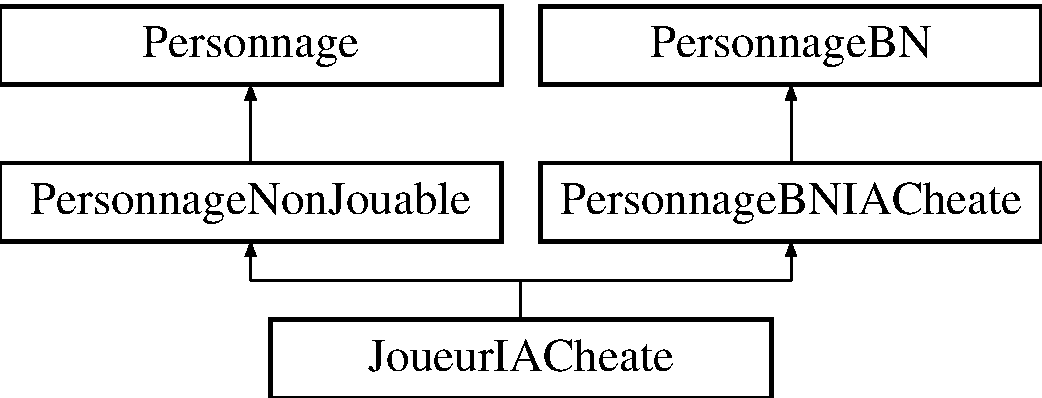
\includegraphics[height=3.000000cm]{classJoueurIACheate}
\end{center}
\end{figure}
\subsection*{Public Member Functions}
\begin{DoxyCompactItemize}
\item 
\hyperlink{classJoueurIACheate_a4a2bd65669ffbd12dbdaf7b41f99eb7f}{Joueur\-I\-A\-Cheate} (string nomnv)
\begin{DoxyCompactList}\small\item\em Constructeur des perso\-B\-N\-I\-A\-Cheate. \end{DoxyCompactList}\item 
\hyperlink{classJoueurIACheate_a0f8fea6f2048e5117eed084e721c5837}{Joueur\-I\-A\-Cheate} (string nomnv, int l, int h, \hyperlink{classArme}{Arme} $\ast$a)
\begin{DoxyCompactList}\small\item\em Constructeur (très) parametre de personnage\-B\-N\-I\-A\-Cheate. \end{DoxyCompactList}\item 
\hyperlink{classJoueurIACheate_a7b59ccf042ba34870d1aa5dd20adc500}{Joueur\-I\-A\-Cheate} (string nomnv, \hyperlink{classArme}{Arme} $\ast$a)
\begin{DoxyCompactList}\small\item\em Constructeur (très) parametre de personnage\-B\-N\-I\-A\-Cheate. \end{DoxyCompactList}\item 
\hyperlink{classJoueurIACheate_aef7db0a97f84a38195e234fddae1cdfd}{Joueur\-I\-A\-Cheate} (string nomnv, int l, int h)
\begin{DoxyCompactList}\small\item\em Constructeur (très) parametre de personnage\-B\-N\-I\-A\-Cheate. \end{DoxyCompactList}\item 
\hyperlink{classJoueurIACheate_a1a624700462855ce07e76d67635cf6d1}{Joueur\-I\-A\-Cheate} (string nomnv, vector$<$ int $>$ t\-Bateaux)
\begin{DoxyCompactList}\small\item\em Constructeur des perso\-B\-N\-I\-A\-Cheate. \end{DoxyCompactList}\item 
\hyperlink{classJoueurIACheate_a0f8cf02fd17baa904d8a2b481fa7923a}{Joueur\-I\-A\-Cheate} (string nomnv, int l, int h, vector$<$ int $>$ t\-Bateaux, \hyperlink{classArme}{Arme} $\ast$a)
\begin{DoxyCompactList}\small\item\em Constructeur (très) parametre de personnage\-B\-N\-I\-A\-Cheate. \end{DoxyCompactList}\item 
\hyperlink{classJoueurIACheate_ac53e64f5fb7b3c616738abbd28321ce5}{Joueur\-I\-A\-Cheate} (string nomnv, vector$<$ int $>$ t\-Bateaux, \hyperlink{classArme}{Arme} $\ast$a)
\begin{DoxyCompactList}\small\item\em Constructeur (très) parametre de personnage\-B\-N\-I\-A\-Cheate. \end{DoxyCompactList}\item 
\hyperlink{classJoueurIACheate_a9eea373255db64950f6f0cd593267d4e}{Joueur\-I\-A\-Cheate} (string nomnv, int l, int h, vector$<$ int $>$ t\-Bateaux)
\begin{DoxyCompactList}\small\item\em Constructeur (très) parametre de personnage\-B\-N\-I\-A\-Cheate. \end{DoxyCompactList}\end{DoxyCompactItemize}


\subsection{Detailed Description}
classe définissant un joueur I\-A 

La classe représente un joueur I\-A se déplaçant sur la carte 

\subsection{Constructor \& Destructor Documentation}
\hypertarget{classJoueurIACheate_a4a2bd65669ffbd12dbdaf7b41f99eb7f}{\index{Joueur\-I\-A\-Cheate@{Joueur\-I\-A\-Cheate}!Joueur\-I\-A\-Cheate@{Joueur\-I\-A\-Cheate}}
\index{Joueur\-I\-A\-Cheate@{Joueur\-I\-A\-Cheate}!JoueurIACheate@{Joueur\-I\-A\-Cheate}}
\subsubsection[{Joueur\-I\-A\-Cheate}]{\setlength{\rightskip}{0pt plus 5cm}Joueur\-I\-A\-Cheate\-::\-Joueur\-I\-A\-Cheate (
\begin{DoxyParamCaption}
\item[{string}]{nomnv}
\end{DoxyParamCaption}
)}}\label{classJoueurIACheate_a4a2bd65669ffbd12dbdaf7b41f99eb7f}


Constructeur des perso\-B\-N\-I\-A\-Cheate. 

Constructeur des perso\-B\-N\-I\-A\-Cheate 
\begin{DoxyParams}{Parameters}
{\em nomnv} & \-: nom du joueur \\
\hline
\end{DoxyParams}
\hypertarget{classJoueurIACheate_a0f8fea6f2048e5117eed084e721c5837}{\index{Joueur\-I\-A\-Cheate@{Joueur\-I\-A\-Cheate}!Joueur\-I\-A\-Cheate@{Joueur\-I\-A\-Cheate}}
\index{Joueur\-I\-A\-Cheate@{Joueur\-I\-A\-Cheate}!JoueurIACheate@{Joueur\-I\-A\-Cheate}}
\subsubsection[{Joueur\-I\-A\-Cheate}]{\setlength{\rightskip}{0pt plus 5cm}Joueur\-I\-A\-Cheate\-::\-Joueur\-I\-A\-Cheate (
\begin{DoxyParamCaption}
\item[{string}]{nomnv, }
\item[{int}]{l, }
\item[{int}]{h, }
\item[{{\bf Arme} $\ast$}]{a}
\end{DoxyParamCaption}
)}}\label{classJoueurIACheate_a0f8fea6f2048e5117eed084e721c5837}


Constructeur (très) parametre de personnage\-B\-N\-I\-A\-Cheate. 


\begin{DoxyParams}{Parameters}
{\em nomnv} & \-: nom du personnage \\
\hline
{\em l} & \-: longueur de la grille \\
\hline
{\em h} & \-: hauteur de la grille \\
\hline
{\em a} & \-: pointeur sur l'arme souhaitée \\
\hline
\end{DoxyParams}
\hypertarget{classJoueurIACheate_a7b59ccf042ba34870d1aa5dd20adc500}{\index{Joueur\-I\-A\-Cheate@{Joueur\-I\-A\-Cheate}!Joueur\-I\-A\-Cheate@{Joueur\-I\-A\-Cheate}}
\index{Joueur\-I\-A\-Cheate@{Joueur\-I\-A\-Cheate}!JoueurIACheate@{Joueur\-I\-A\-Cheate}}
\subsubsection[{Joueur\-I\-A\-Cheate}]{\setlength{\rightskip}{0pt plus 5cm}Joueur\-I\-A\-Cheate\-::\-Joueur\-I\-A\-Cheate (
\begin{DoxyParamCaption}
\item[{string}]{nomnv, }
\item[{{\bf Arme} $\ast$}]{a}
\end{DoxyParamCaption}
)}}\label{classJoueurIACheate_a7b59ccf042ba34870d1aa5dd20adc500}


Constructeur (très) parametre de personnage\-B\-N\-I\-A\-Cheate. 


\begin{DoxyParams}{Parameters}
{\em nomnv} & \-: nom du personnage \\
\hline
{\em a} & \-: pointeur sur l'arme souhaitée \\
\hline
\end{DoxyParams}
\hypertarget{classJoueurIACheate_aef7db0a97f84a38195e234fddae1cdfd}{\index{Joueur\-I\-A\-Cheate@{Joueur\-I\-A\-Cheate}!Joueur\-I\-A\-Cheate@{Joueur\-I\-A\-Cheate}}
\index{Joueur\-I\-A\-Cheate@{Joueur\-I\-A\-Cheate}!JoueurIACheate@{Joueur\-I\-A\-Cheate}}
\subsubsection[{Joueur\-I\-A\-Cheate}]{\setlength{\rightskip}{0pt plus 5cm}Joueur\-I\-A\-Cheate\-::\-Joueur\-I\-A\-Cheate (
\begin{DoxyParamCaption}
\item[{string}]{nomnv, }
\item[{int}]{l, }
\item[{int}]{h}
\end{DoxyParamCaption}
)}}\label{classJoueurIACheate_aef7db0a97f84a38195e234fddae1cdfd}


Constructeur (très) parametre de personnage\-B\-N\-I\-A\-Cheate. 


\begin{DoxyParams}{Parameters}
{\em nomnv} & \-: nom du personnage \\
\hline
{\em l} & \-: longueur de la grille \\
\hline
{\em h} & \-: hauteur de la grille \\
\hline
\end{DoxyParams}
\hypertarget{classJoueurIACheate_a1a624700462855ce07e76d67635cf6d1}{\index{Joueur\-I\-A\-Cheate@{Joueur\-I\-A\-Cheate}!Joueur\-I\-A\-Cheate@{Joueur\-I\-A\-Cheate}}
\index{Joueur\-I\-A\-Cheate@{Joueur\-I\-A\-Cheate}!JoueurIACheate@{Joueur\-I\-A\-Cheate}}
\subsubsection[{Joueur\-I\-A\-Cheate}]{\setlength{\rightskip}{0pt plus 5cm}Joueur\-I\-A\-Cheate\-::\-Joueur\-I\-A\-Cheate (
\begin{DoxyParamCaption}
\item[{string}]{nomnv, }
\item[{vector$<$ int $>$}]{t\-Bateaux}
\end{DoxyParamCaption}
)}}\label{classJoueurIACheate_a1a624700462855ce07e76d67635cf6d1}


Constructeur des perso\-B\-N\-I\-A\-Cheate. 

Constructeur des perso\-B\-N\-I\-A\-Cheate 
\begin{DoxyParams}{Parameters}
{\em t\-Bateaux} & \-: vector de taille de bateaux \\
\hline
{\em nomnv} & \-: nom du joueur \\
\hline
\end{DoxyParams}
\hypertarget{classJoueurIACheate_a0f8cf02fd17baa904d8a2b481fa7923a}{\index{Joueur\-I\-A\-Cheate@{Joueur\-I\-A\-Cheate}!Joueur\-I\-A\-Cheate@{Joueur\-I\-A\-Cheate}}
\index{Joueur\-I\-A\-Cheate@{Joueur\-I\-A\-Cheate}!JoueurIACheate@{Joueur\-I\-A\-Cheate}}
\subsubsection[{Joueur\-I\-A\-Cheate}]{\setlength{\rightskip}{0pt plus 5cm}Joueur\-I\-A\-Cheate\-::\-Joueur\-I\-A\-Cheate (
\begin{DoxyParamCaption}
\item[{string}]{nomnv, }
\item[{int}]{l, }
\item[{int}]{h, }
\item[{vector$<$ int $>$}]{t\-Bateaux, }
\item[{{\bf Arme} $\ast$}]{a}
\end{DoxyParamCaption}
)}}\label{classJoueurIACheate_a0f8cf02fd17baa904d8a2b481fa7923a}


Constructeur (très) parametre de personnage\-B\-N\-I\-A\-Cheate. 


\begin{DoxyParams}{Parameters}
{\em nomnv} & \-: nom du personnage \\
\hline
{\em t\-Bateaux} & \-: vector de taille de bateaux \\
\hline
{\em l} & \-: longueur de la grille \\
\hline
{\em h} & \-: hauteur de la grille \\
\hline
{\em a} & \-: pointeur sur l'arme souhaitée \\
\hline
\end{DoxyParams}
\hypertarget{classJoueurIACheate_ac53e64f5fb7b3c616738abbd28321ce5}{\index{Joueur\-I\-A\-Cheate@{Joueur\-I\-A\-Cheate}!Joueur\-I\-A\-Cheate@{Joueur\-I\-A\-Cheate}}
\index{Joueur\-I\-A\-Cheate@{Joueur\-I\-A\-Cheate}!JoueurIACheate@{Joueur\-I\-A\-Cheate}}
\subsubsection[{Joueur\-I\-A\-Cheate}]{\setlength{\rightskip}{0pt plus 5cm}Joueur\-I\-A\-Cheate\-::\-Joueur\-I\-A\-Cheate (
\begin{DoxyParamCaption}
\item[{string}]{nomnv, }
\item[{vector$<$ int $>$}]{t\-Bateaux, }
\item[{{\bf Arme} $\ast$}]{a}
\end{DoxyParamCaption}
)}}\label{classJoueurIACheate_ac53e64f5fb7b3c616738abbd28321ce5}


Constructeur (très) parametre de personnage\-B\-N\-I\-A\-Cheate. 


\begin{DoxyParams}{Parameters}
{\em t\-Bateaux} & \-: vector de taille de bateaux \\
\hline
{\em nomnv} & \-: nom du personnage \\
\hline
{\em a} & \-: pointeur sur l'arme souhaitée \\
\hline
\end{DoxyParams}
\hypertarget{classJoueurIACheate_a9eea373255db64950f6f0cd593267d4e}{\index{Joueur\-I\-A\-Cheate@{Joueur\-I\-A\-Cheate}!Joueur\-I\-A\-Cheate@{Joueur\-I\-A\-Cheate}}
\index{Joueur\-I\-A\-Cheate@{Joueur\-I\-A\-Cheate}!JoueurIACheate@{Joueur\-I\-A\-Cheate}}
\subsubsection[{Joueur\-I\-A\-Cheate}]{\setlength{\rightskip}{0pt plus 5cm}Joueur\-I\-A\-Cheate\-::\-Joueur\-I\-A\-Cheate (
\begin{DoxyParamCaption}
\item[{string}]{nomnv, }
\item[{int}]{l, }
\item[{int}]{h, }
\item[{vector$<$ int $>$}]{t\-Bateaux}
\end{DoxyParamCaption}
)}}\label{classJoueurIACheate_a9eea373255db64950f6f0cd593267d4e}


Constructeur (très) parametre de personnage\-B\-N\-I\-A\-Cheate. 


\begin{DoxyParams}{Parameters}
{\em nomnv} & \-: nom du personnage \\
\hline
{\em t\-Bateaux} & \-: vector de taille de bateaux \\
\hline
{\em l} & \-: longueur de la grille \\
\hline
{\em h} & \-: hauteur de la grille \\
\hline
\end{DoxyParams}


The documentation for this class was generated from the following files\-:\begin{DoxyCompactItemize}
\item 
/home/damien/\-Bureau/projetcpp\-\_\-gm42/source/src/\hyperlink{JoueurIACheate_8hpp}{Joueur\-I\-A\-Cheate.\-hpp}\item 
/home/damien/\-Bureau/projetcpp\-\_\-gm42/source/src/Joueur\-I\-A\-Cheate.\-cpp\end{DoxyCompactItemize}

\hypertarget{classMonde}{\section{Monde Class Reference}
\label{classMonde}\index{Monde@{Monde}}
}


classe définissant un monde  




{\ttfamily \#include $<$Monde.\-hpp$>$}

\subsection*{Public Member Functions}
\begin{DoxyCompactItemize}
\item 
\hyperlink{classMonde_a7749057a35c8a337c567640313a5e259}{Monde} ()
\begin{DoxyCompactList}\small\item\em Constructeur par défaut. \end{DoxyCompactList}\item 
\hyperlink{classCarte}{Carte} $\ast$ \hyperlink{classMonde_adee77b23396e207285f4205fe62ae74d}{get\-Carte} (int id)
\begin{DoxyCompactList}\small\item\em getter \end{DoxyCompactList}\end{DoxyCompactItemize}


\subsection{Detailed Description}
classe définissant un monde 

La classe représente un monde constitué de carte sur lequel évolue le joueur 

\subsection{Constructor \& Destructor Documentation}
\hypertarget{classMonde_a7749057a35c8a337c567640313a5e259}{\index{Monde@{Monde}!Monde@{Monde}}
\index{Monde@{Monde}!Monde@{Monde}}
\subsubsection[{Monde}]{\setlength{\rightskip}{0pt plus 5cm}Monde\-::\-Monde (
\begin{DoxyParamCaption}
{}
\end{DoxyParamCaption}
)}}\label{classMonde_a7749057a35c8a337c567640313a5e259}


Constructeur par défaut. 

Constructeur de la classe \hyperlink{classMonde}{Monde} par défaut 

\subsection{Member Function Documentation}
\hypertarget{classMonde_adee77b23396e207285f4205fe62ae74d}{\index{Monde@{Monde}!get\-Carte@{get\-Carte}}
\index{get\-Carte@{get\-Carte}!Monde@{Monde}}
\subsubsection[{get\-Carte}]{\setlength{\rightskip}{0pt plus 5cm}{\bf Carte} $\ast$ Monde\-::get\-Carte (
\begin{DoxyParamCaption}
\item[{int}]{id}
\end{DoxyParamCaption}
)}}\label{classMonde_adee77b23396e207285f4205fe62ae74d}


getter 


\begin{DoxyParams}{Parameters}
{\em id} & \-: numero de la carte \\
\hline
\end{DoxyParams}


The documentation for this class was generated from the following files\-:\begin{DoxyCompactItemize}
\item 
/home/damien/\-Bureau/projetcpp\-\_\-gm42/source/src/\hyperlink{Monde_8hpp}{Monde.\-hpp}\item 
/home/damien/\-Bureau/projetcpp\-\_\-gm42/source/src/Monde.\-cpp\end{DoxyCompactItemize}

\hypertarget{classObjet}{\section{Objet Class Reference}
\label{classObjet}\index{Objet@{Objet}}
}


Gestion des objets.  




{\ttfamily \#include $<$Objet.\-hpp$>$}

Inheritance diagram for Objet\-:\begin{figure}[H]
\begin{center}
\leavevmode
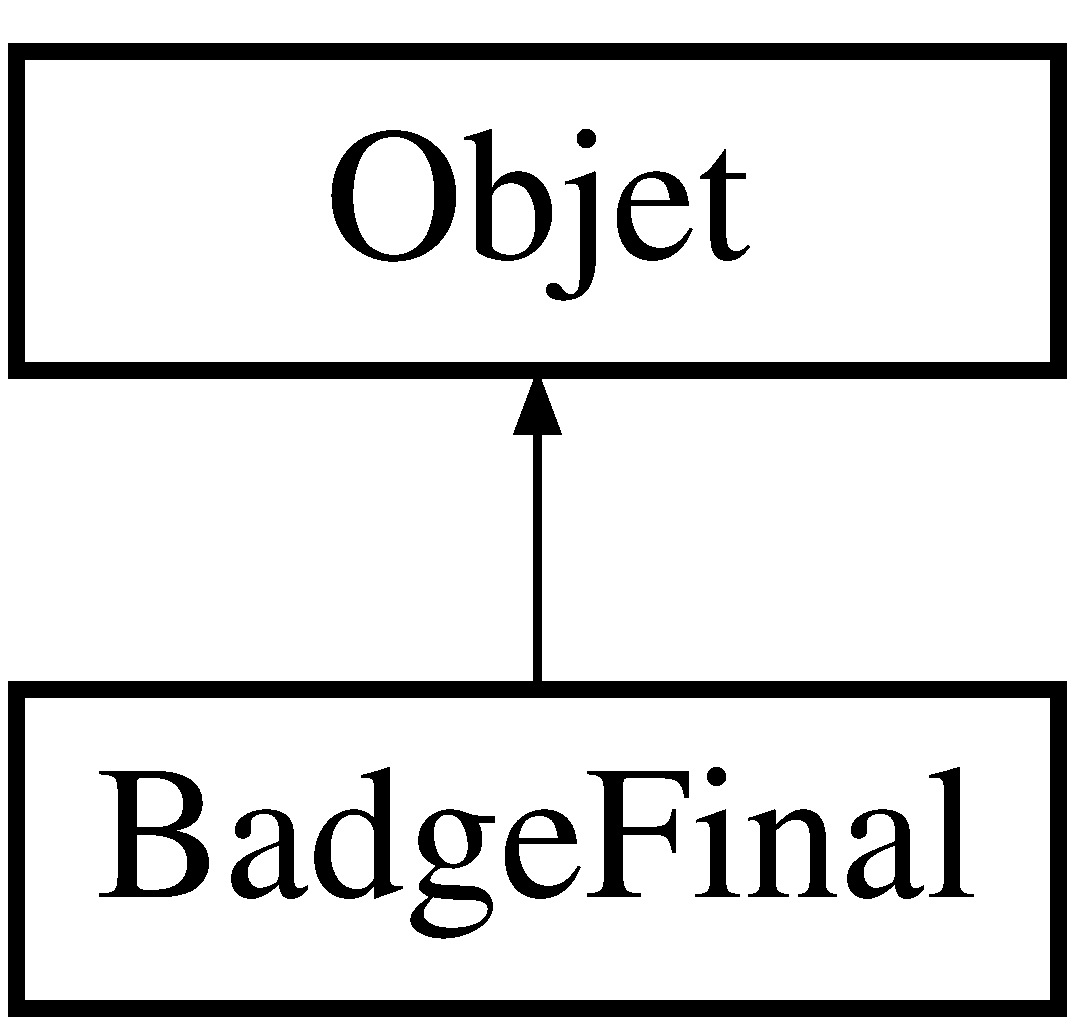
\includegraphics[height=2.000000cm]{classObjet}
\end{center}
\end{figure}
\subsection*{Public Member Functions}
\begin{DoxyCompactItemize}
\item 
\hyperlink{classObjet_ab9b72f8c1cb2af52c0b9e334126c361e}{Objet} (const string nom\-Objet)
\begin{DoxyCompactList}\small\item\em constructeur parametré de \hyperlink{classObjet}{Objet} \end{DoxyCompactList}\item 
\hypertarget{classObjet_ae69f82c5eb6d573032ac1f6e548cdb00}{string \hyperlink{classObjet_ae69f82c5eb6d573032ac1f6e548cdb00}{get\-Nom} () const }\label{classObjet_ae69f82c5eb6d573032ac1f6e548cdb00}

\begin{DoxyCompactList}\small\item\em Getter du nom de l'objet. \end{DoxyCompactList}\item 
\hypertarget{classObjet_ad25b7793754858f839119f0c812fc9b8}{virtual bool \hyperlink{classObjet_ad25b7793754858f839119f0c812fc9b8}{met\-Fin\-Au\-Jeu} () const =0}\label{classObjet_ad25b7793754858f839119f0c812fc9b8}

\begin{DoxyCompactList}\small\item\em Methode Virtuelle pure retournant si l'objet. \end{DoxyCompactList}\end{DoxyCompactItemize}


\subsection{Detailed Description}
Gestion des objets. 

Cette classe gère les informations concernant les objets de l'inventaire 

\subsection{Constructor \& Destructor Documentation}
\hypertarget{classObjet_ab9b72f8c1cb2af52c0b9e334126c361e}{\index{Objet@{Objet}!Objet@{Objet}}
\index{Objet@{Objet}!Objet@{Objet}}
\subsubsection[{Objet}]{\setlength{\rightskip}{0pt plus 5cm}Objet\-::\-Objet (
\begin{DoxyParamCaption}
\item[{const string}]{nom\-Objet}
\end{DoxyParamCaption}
)}}\label{classObjet_ab9b72f8c1cb2af52c0b9e334126c361e}


constructeur parametré de \hyperlink{classObjet}{Objet} 


\begin{DoxyParams}{Parameters}
{\em nom\-Objet} & \-: Le nom de l'objet \\
\hline
\end{DoxyParams}


The documentation for this class was generated from the following files\-:\begin{DoxyCompactItemize}
\item 
/home/damien/\-Bureau/projetcpp\-\_\-gm42/source/src/\hyperlink{Objet_8hpp}{Objet.\-hpp}\item 
/home/damien/\-Bureau/projetcpp\-\_\-gm42/source/src/Objet.\-cpp\end{DoxyCompactItemize}

\hypertarget{classPersonnage}{\section{Personnage Class Reference}
\label{classPersonnage}\index{Personnage@{Personnage}}
}


classe définissant un personnage  




{\ttfamily \#include $<$Personnage.\-hpp$>$}

Inheritance diagram for Personnage\-:\begin{figure}[H]
\begin{center}
\leavevmode
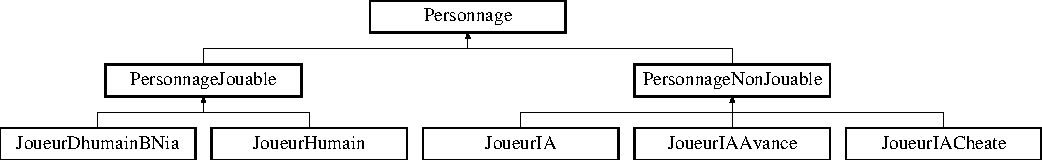
\includegraphics[height=2.153846cm]{classPersonnage}
\end{center}
\end{figure}
\subsection*{Public Member Functions}
\begin{DoxyCompactItemize}
\item 
\hyperlink{classPersonnage_a93723cd22a0b4c2e6edd62e07e09a745}{Personnage} (string nomnv)
\begin{DoxyCompactList}\small\item\em constructeur \end{DoxyCompactList}\item 
void \hyperlink{classPersonnage_a91f650f5ede9c187560dd5c03907b337}{deplacer} (\hyperlink{classCoordonnees}{Coordonnees} coordonnees, \hyperlink{classCarte}{Carte} $\ast$carte\-Entree)
\begin{DoxyCompactList}\small\item\em fonction déplacer \end{DoxyCompactList}\item 
\hyperlink{classCoordonnees}{Coordonnees} \hyperlink{classPersonnage_ae66327fd2d09e133d049f96e6b3a68cf}{get\-Coordonnees} () const 
\begin{DoxyCompactList}\small\item\em Getter \hyperlink{classCoordonnees}{Coordonnees}. \end{DoxyCompactList}\item 
\hyperlink{classCarte}{Carte} $\ast$ \hyperlink{classPersonnage_a9c4fd5657f04f3b9defc603fc05b99da}{get\-Carte} () const 
\begin{DoxyCompactList}\small\item\em Getter \hyperlink{classCarte}{Carte}. \end{DoxyCompactList}\item 
string \hyperlink{classPersonnage_ad05ce70497e8321d81795776a5b77948}{get\-Nom} () const 
\begin{DoxyCompactList}\small\item\em Getter Nom. \end{DoxyCompactList}\item 
void \hyperlink{classPersonnage_a13269350d46d0a5a32454b51b5dce7af}{set\-Coordonnees} (\hyperlink{classCoordonnees}{Coordonnees} coord\-Set)
\begin{DoxyCompactList}\small\item\em Setter \hyperlink{classCoordonnees}{Coordonnees}. \end{DoxyCompactList}\item 
void \hyperlink{classPersonnage_afd695f3d63d2a1093476997230e3a055}{set\-Carte} (\hyperlink{classCarte}{Carte} $\ast$carte\-Set)
\begin{DoxyCompactList}\small\item\em Setter \hyperlink{classCarte}{Carte}. \end{DoxyCompactList}\item 
\hyperlink{classInventaire}{Inventaire} $\ast$ \hyperlink{classPersonnage_a1ec8306749f543f4396d511bb8b80621}{get\-Inventaire} ()
\begin{DoxyCompactList}\small\item\em Getter \hyperlink{classInventaire}{Inventaire}. \end{DoxyCompactList}\end{DoxyCompactItemize}


\subsection{Detailed Description}
classe définissant un personnage 

La classe représente un personnage du jeu, contrôlable ou non, humain ou non 

\subsection{Constructor \& Destructor Documentation}
\hypertarget{classPersonnage_a93723cd22a0b4c2e6edd62e07e09a745}{\index{Personnage@{Personnage}!Personnage@{Personnage}}
\index{Personnage@{Personnage}!Personnage@{Personnage}}
\subsubsection[{Personnage}]{\setlength{\rightskip}{0pt plus 5cm}Personnage\-::\-Personnage (
\begin{DoxyParamCaption}
\item[{string}]{nomnv}
\end{DoxyParamCaption}
)}}\label{classPersonnage_a93723cd22a0b4c2e6edd62e07e09a745}


constructeur 


\begin{DoxyParams}{Parameters}
{\em nomnv} & \-: nom du joueur \\
\hline
\end{DoxyParams}


\subsection{Member Function Documentation}
\hypertarget{classPersonnage_a91f650f5ede9c187560dd5c03907b337}{\index{Personnage@{Personnage}!deplacer@{deplacer}}
\index{deplacer@{deplacer}!Personnage@{Personnage}}
\subsubsection[{deplacer}]{\setlength{\rightskip}{0pt plus 5cm}void Personnage\-::deplacer (
\begin{DoxyParamCaption}
\item[{{\bf Coordonnees}}]{coordonnees, }
\item[{{\bf Carte} $\ast$}]{carte}
\end{DoxyParamCaption}
)}}\label{classPersonnage_a91f650f5ede9c187560dd5c03907b337}


fonction déplacer 

Permet le déplacement d'un personnage sur la carte et les coordonnées en entrée 
\begin{DoxyParams}{Parameters}
{\em coordonnees} & \-: coordonnées de destination \\
\hline
{\em carte} & \-: pointeur sur la carte de destination \\
\hline
\end{DoxyParams}
\hypertarget{classPersonnage_a9c4fd5657f04f3b9defc603fc05b99da}{\index{Personnage@{Personnage}!get\-Carte@{get\-Carte}}
\index{get\-Carte@{get\-Carte}!Personnage@{Personnage}}
\subsubsection[{get\-Carte}]{\setlength{\rightskip}{0pt plus 5cm}{\bf Carte} Personnage\-::get\-Carte (
\begin{DoxyParamCaption}
{}
\end{DoxyParamCaption}
) const}}\label{classPersonnage_a9c4fd5657f04f3b9defc603fc05b99da}


Getter \hyperlink{classCarte}{Carte}. 

\begin{DoxyReturn}{Returns}
Un pointeur sur la carte du personnage 
\end{DoxyReturn}
\hypertarget{classPersonnage_ae66327fd2d09e133d049f96e6b3a68cf}{\index{Personnage@{Personnage}!get\-Coordonnees@{get\-Coordonnees}}
\index{get\-Coordonnees@{get\-Coordonnees}!Personnage@{Personnage}}
\subsubsection[{get\-Coordonnees}]{\setlength{\rightskip}{0pt plus 5cm}{\bf Coordonnees} Personnage\-::get\-Coordonnees (
\begin{DoxyParamCaption}
{}
\end{DoxyParamCaption}
) const}}\label{classPersonnage_ae66327fd2d09e133d049f96e6b3a68cf}


Getter \hyperlink{classCoordonnees}{Coordonnees}. 

\begin{DoxyReturn}{Returns}
Les coordonnees du personnage 
\end{DoxyReturn}
\hypertarget{classPersonnage_a1ec8306749f543f4396d511bb8b80621}{\index{Personnage@{Personnage}!get\-Inventaire@{get\-Inventaire}}
\index{get\-Inventaire@{get\-Inventaire}!Personnage@{Personnage}}
\subsubsection[{get\-Inventaire}]{\setlength{\rightskip}{0pt plus 5cm}{\bf Inventaire} $\ast$ Personnage\-::get\-Inventaire (
\begin{DoxyParamCaption}
{}
\end{DoxyParamCaption}
)}}\label{classPersonnage_a1ec8306749f543f4396d511bb8b80621}


Getter \hyperlink{classInventaire}{Inventaire}. 

\begin{DoxyReturn}{Returns}
l'inventaire du personnage 
\end{DoxyReturn}
\hypertarget{classPersonnage_ad05ce70497e8321d81795776a5b77948}{\index{Personnage@{Personnage}!get\-Nom@{get\-Nom}}
\index{get\-Nom@{get\-Nom}!Personnage@{Personnage}}
\subsubsection[{get\-Nom}]{\setlength{\rightskip}{0pt plus 5cm}string Personnage\-::get\-Nom (
\begin{DoxyParamCaption}
{}
\end{DoxyParamCaption}
) const}}\label{classPersonnage_ad05ce70497e8321d81795776a5b77948}


Getter Nom. 

\begin{DoxyReturn}{Returns}
Le nom du joueur 
\end{DoxyReturn}
\hypertarget{classPersonnage_afd695f3d63d2a1093476997230e3a055}{\index{Personnage@{Personnage}!set\-Carte@{set\-Carte}}
\index{set\-Carte@{set\-Carte}!Personnage@{Personnage}}
\subsubsection[{set\-Carte}]{\setlength{\rightskip}{0pt plus 5cm}void Personnage\-::set\-Carte (
\begin{DoxyParamCaption}
\item[{{\bf Carte} $\ast$}]{carte\-Set}
\end{DoxyParamCaption}
)}}\label{classPersonnage_afd695f3d63d2a1093476997230e3a055}


Setter \hyperlink{classCarte}{Carte}. 


\begin{DoxyParams}{Parameters}
{\em carte\-Set} & \-: la carte à pointer en attribut \\
\hline
\end{DoxyParams}
\hypertarget{classPersonnage_a13269350d46d0a5a32454b51b5dce7af}{\index{Personnage@{Personnage}!set\-Coordonnees@{set\-Coordonnees}}
\index{set\-Coordonnees@{set\-Coordonnees}!Personnage@{Personnage}}
\subsubsection[{set\-Coordonnees}]{\setlength{\rightskip}{0pt plus 5cm}vodi Personnage\-::set\-Coordonnees (
\begin{DoxyParamCaption}
\item[{{\bf Coordonnees}}]{coord\-Set}
\end{DoxyParamCaption}
)}}\label{classPersonnage_a13269350d46d0a5a32454b51b5dce7af}


Setter \hyperlink{classCoordonnees}{Coordonnees}. 


\begin{DoxyParams}{Parameters}
{\em coord\-Set} & Les coordonnees du personnage \\
\hline
\end{DoxyParams}


The documentation for this class was generated from the following files\-:\begin{DoxyCompactItemize}
\item 
/home/damien/\-Bureau/projetcpp\-\_\-gm42/source/src/\hyperlink{Personnage_8hpp}{Personnage.\-hpp}\item 
/home/damien/\-Bureau/projetcpp\-\_\-gm42/source/src/Personnage.\-cpp\end{DoxyCompactItemize}

\hypertarget{classPersonnageBN}{\section{Personnage\-B\-N Class Reference}
\label{classPersonnageBN}\index{Personnage\-B\-N@{Personnage\-B\-N}}
}


\hyperlink{classPersonnage}{Personnage} pouvant jouer au combat\-: \hyperlink{classBatailleNavale}{Bataille\-Navale}.  




{\ttfamily \#include $<$Personnage\-B\-N.\-hpp$>$}

Inheritance diagram for Personnage\-B\-N\-:\begin{figure}[H]
\begin{center}
\leavevmode
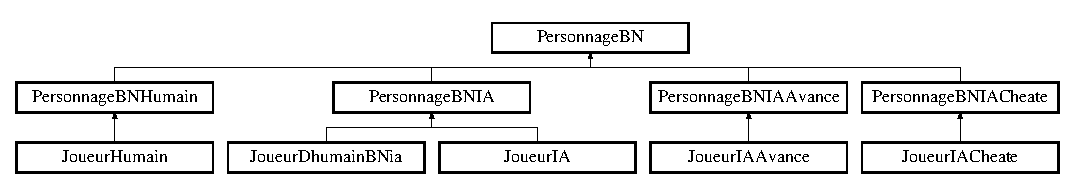
\includegraphics[height=2.086957cm]{classPersonnageBN}
\end{center}
\end{figure}
\subsection*{Public Member Functions}
\begin{DoxyCompactItemize}
\item 
\hyperlink{classPersonnageBN_a09564d1f60e3e8ac05e7197cf886d45c}{Personnage\-B\-N} (string nomnv)
\begin{DoxyCompactList}\small\item\em Constructeur des perso\-B\-N. \end{DoxyCompactList}\item 
\hyperlink{classPersonnageBN_a6391c5c85d03608e309883c965638de5}{Personnage\-B\-N} (string nomnv, int l, int h, \hyperlink{classArme}{Arme} $\ast$a)
\begin{DoxyCompactList}\small\item\em Constructeur (très) parametre de personnage\-B\-N. \end{DoxyCompactList}\item 
\hyperlink{classPersonnageBN_af5a557a3a1114ef67ac5ac37ffec6d8a}{Personnage\-B\-N} (string nomnv, \hyperlink{classArme}{Arme} $\ast$a)
\begin{DoxyCompactList}\small\item\em Constructeur (très) parametre de personnage\-B\-N. \end{DoxyCompactList}\item 
\hyperlink{classPersonnageBN_aa5b7ac10ef5611e0e869a681c2cda915}{Personnage\-B\-N} (string nomnv, int l, int h)
\begin{DoxyCompactList}\small\item\em Constructeur (très) parametre de personnage\-B\-N. \end{DoxyCompactList}\item 
\hyperlink{classPersonnageBN_ae701e953e890a4168268f003b44c886f}{Personnage\-B\-N} (string nomnv, vector$<$ int $>$ t\-Bateaux)
\begin{DoxyCompactList}\small\item\em Constructeur des perso\-B\-N. \end{DoxyCompactList}\item 
\hyperlink{classPersonnageBN_a24f6e9b0b2ce83fdd3d49e77fac63ce3}{Personnage\-B\-N} (string nomnv, int l, int h, vector$<$ int $>$ t\-Bateaux, \hyperlink{classArme}{Arme} $\ast$a)
\begin{DoxyCompactList}\small\item\em Constructeur (très) parametre de personnage\-B\-N. \end{DoxyCompactList}\item 
\hyperlink{classPersonnageBN_a49265459e63c0bea4f9dfb702dd76c40}{Personnage\-B\-N} (string nomnv, vector$<$ int $>$ t\-Bateaux, \hyperlink{classArme}{Arme} $\ast$a)
\begin{DoxyCompactList}\small\item\em Constructeur (très) parametre de personnage\-B\-N. \end{DoxyCompactList}\item 
\hyperlink{classPersonnageBN_ad0c724004d5896a6ca9bd3501c432039}{Personnage\-B\-N} (string nomnv, int l, int h, vector$<$ int $>$ t\-Bateaux)
\begin{DoxyCompactList}\small\item\em Constructeur (très) parametre de personnage\-B\-N. \end{DoxyCompactList}\item 
\hyperlink{classTailleGrille}{Taille\-Grille} \hyperlink{classPersonnageBN_a79d3d1e8c0b174ac9659edb26787380d}{get\-Taille\-Grille} () const 
\begin{DoxyCompactList}\small\item\em getters de taille\-Grille \end{DoxyCompactList}\item 
void \hyperlink{classPersonnageBN_a00256daec53f83cd70540647cdff2fa8}{ajouter\-Bateau} (const int taille)
\begin{DoxyCompactList}\small\item\em Ajoute un baeatu à la flotte. \end{DoxyCompactList}\item 
string \hyperlink{classPersonnageBN_af8957d888f3065180f12919ff6a04948}{get\-Nom\-B\-N} () const 
\begin{DoxyCompactList}\small\item\em getters du nom\-B\-N \end{DoxyCompactList}\item 
void \hyperlink{classPersonnageBN_a5b63a8a11fbb52a26c8aa29407dc2071}{set\-Nom\-B\-N} (const string nvnom)
\begin{DoxyCompactList}\small\item\em Setter du nom\-B\-N. \end{DoxyCompactList}\item 
\hyperlink{classArme}{Arme} $\ast$ \hyperlink{classPersonnageBN_a6ff27cfd1a82e6127accfcfebd09be08}{get\-Arme} () const 
\begin{DoxyCompactList}\small\item\em getters du pointeur sur \hyperlink{classArme}{Arme} \end{DoxyCompactList}\item 
vector$<$ \hyperlink{classBateau}{Bateau} $\ast$ $>$ \hyperlink{classPersonnageBN_a7f230cf0537de207fcc170f9663e8c6b}{get\-Bateaux} () const 
\begin{DoxyCompactList}\small\item\em getters du vecteur de pointeurs sur Bateaux \end{DoxyCompactList}\item 
void \hyperlink{classPersonnageBN_a41cd6da402ac37e5631942ca5156420c}{set\-Taille\-Grille} (const \hyperlink{classTailleGrille}{Taille\-Grille} tg)
\begin{DoxyCompactList}\small\item\em setters de taille\-Grille \end{DoxyCompactList}\item 
void \hyperlink{classPersonnageBN_a2d9befe652ed12cc68451a6855dac07e}{set\-Arme} (\hyperlink{classArme}{Arme} $\ast$nv\-Arme)
\begin{DoxyCompactList}\small\item\em setters d'\hyperlink{classArme}{Arme} \end{DoxyCompactList}\item 
void \hyperlink{classPersonnageBN_aded99fbc0a1314128d435ee8095d78b8}{set\-Bateaux} (const vector$<$ \hyperlink{classBateau}{Bateau} $\ast$ $>$ nv\-Bateaux)
\begin{DoxyCompactList}\small\item\em setters de bateaux \end{DoxyCompactList}\item 
virtual \hyperlink{classGrille}{Grille} \hyperlink{classPersonnageBN_a72b5b94a8e06f39c608c7310d4785579}{placer\-Bateaux} ()=0
\begin{DoxyCompactList}\small\item\em le \hyperlink{classPersonnageBN}{Personnage\-B\-N} place les Bateaux sur sa \hyperlink{classGrille}{Grille} \end{DoxyCompactList}\item 
virtual \hyperlink{classCoordonnees}{Coordonnees} \hyperlink{classPersonnageBN_aaf4e97d763adba22bc5a89b2537e6dbe}{coordonnees\-A\-Viser} (\hyperlink{classGrille}{Grille} $\ast$grille\-Adverse)=0
\begin{DoxyCompactList}\small\item\em le \hyperlink{classPersonnageBN}{Personnage\-B\-N} veux tirer sur la grille du joueur adverse \end{DoxyCompactList}\item 
void \hyperlink{classPersonnageBN_a6d8837669e41914b1494d040e455ee1d}{restaurer\-Bateaux} ()
\begin{DoxyCompactList}\small\item\em restaure les P\-V des bateaux \end{DoxyCompactList}\item 
bool \hyperlink{classPersonnageBN_ad8fb6423ac3e2b7f48348eb3b7a9992e}{flotte\-Coulee} ()
\begin{DoxyCompactList}\small\item\em verifie si la flotte est coulee \end{DoxyCompactList}\end{DoxyCompactItemize}


\subsection{Detailed Description}
\hyperlink{classPersonnage}{Personnage} pouvant jouer au combat\-: \hyperlink{classBatailleNavale}{Bataille\-Navale}. 

\subsection{Constructor \& Destructor Documentation}
\hypertarget{classPersonnageBN_a09564d1f60e3e8ac05e7197cf886d45c}{\index{Personnage\-B\-N@{Personnage\-B\-N}!Personnage\-B\-N@{Personnage\-B\-N}}
\index{Personnage\-B\-N@{Personnage\-B\-N}!PersonnageBN@{Personnage\-B\-N}}
\subsubsection[{Personnage\-B\-N}]{\setlength{\rightskip}{0pt plus 5cm}Personnage\-B\-N\-::\-Personnage\-B\-N (
\begin{DoxyParamCaption}
\item[{string}]{nomnv}
\end{DoxyParamCaption}
)}}\label{classPersonnageBN_a09564d1f60e3e8ac05e7197cf886d45c}


Constructeur des perso\-B\-N. 

Constructeur des perso\-B\-N 
\begin{DoxyParams}{Parameters}
{\em nomnv} & \-: nom du joueur \\
\hline
\end{DoxyParams}
\hypertarget{classPersonnageBN_a6391c5c85d03608e309883c965638de5}{\index{Personnage\-B\-N@{Personnage\-B\-N}!Personnage\-B\-N@{Personnage\-B\-N}}
\index{Personnage\-B\-N@{Personnage\-B\-N}!PersonnageBN@{Personnage\-B\-N}}
\subsubsection[{Personnage\-B\-N}]{\setlength{\rightskip}{0pt plus 5cm}Personnage\-B\-N\-::\-Personnage\-B\-N (
\begin{DoxyParamCaption}
\item[{string}]{nomnv, }
\item[{int}]{l, }
\item[{int}]{h, }
\item[{{\bf Arme} $\ast$}]{a}
\end{DoxyParamCaption}
)}}\label{classPersonnageBN_a6391c5c85d03608e309883c965638de5}


Constructeur (très) parametre de personnage\-B\-N. 


\begin{DoxyParams}{Parameters}
{\em nomnv} & \-: nom du personnage \\
\hline
{\em l} & \-: longueur de la grille \\
\hline
{\em h} & \-: hauteur de la grille \\
\hline
{\em a} & \-: pointeur sur l'arme souhaitée \\
\hline
\end{DoxyParams}
\hypertarget{classPersonnageBN_af5a557a3a1114ef67ac5ac37ffec6d8a}{\index{Personnage\-B\-N@{Personnage\-B\-N}!Personnage\-B\-N@{Personnage\-B\-N}}
\index{Personnage\-B\-N@{Personnage\-B\-N}!PersonnageBN@{Personnage\-B\-N}}
\subsubsection[{Personnage\-B\-N}]{\setlength{\rightskip}{0pt plus 5cm}Personnage\-B\-N\-::\-Personnage\-B\-N (
\begin{DoxyParamCaption}
\item[{string}]{nomnv, }
\item[{{\bf Arme} $\ast$}]{a}
\end{DoxyParamCaption}
)}}\label{classPersonnageBN_af5a557a3a1114ef67ac5ac37ffec6d8a}


Constructeur (très) parametre de personnage\-B\-N. 


\begin{DoxyParams}{Parameters}
{\em nomnv} & \-: nom du personnage \\
\hline
{\em a} & \-: pointeur sur l'arme souhaitée \\
\hline
\end{DoxyParams}
\hypertarget{classPersonnageBN_aa5b7ac10ef5611e0e869a681c2cda915}{\index{Personnage\-B\-N@{Personnage\-B\-N}!Personnage\-B\-N@{Personnage\-B\-N}}
\index{Personnage\-B\-N@{Personnage\-B\-N}!PersonnageBN@{Personnage\-B\-N}}
\subsubsection[{Personnage\-B\-N}]{\setlength{\rightskip}{0pt plus 5cm}Personnage\-B\-N\-::\-Personnage\-B\-N (
\begin{DoxyParamCaption}
\item[{string}]{nomnv, }
\item[{int}]{l, }
\item[{int}]{h}
\end{DoxyParamCaption}
)}}\label{classPersonnageBN_aa5b7ac10ef5611e0e869a681c2cda915}


Constructeur (très) parametre de personnage\-B\-N. 


\begin{DoxyParams}{Parameters}
{\em nomnv} & \-: nom du personnage \\
\hline
{\em l} & \-: longueur de la grille \\
\hline
{\em h} & \-: hauteur de la grille \\
\hline
\end{DoxyParams}
\hypertarget{classPersonnageBN_ae701e953e890a4168268f003b44c886f}{\index{Personnage\-B\-N@{Personnage\-B\-N}!Personnage\-B\-N@{Personnage\-B\-N}}
\index{Personnage\-B\-N@{Personnage\-B\-N}!PersonnageBN@{Personnage\-B\-N}}
\subsubsection[{Personnage\-B\-N}]{\setlength{\rightskip}{0pt plus 5cm}Personnage\-B\-N\-::\-Personnage\-B\-N (
\begin{DoxyParamCaption}
\item[{string}]{nomnv, }
\item[{vector$<$ int $>$}]{t\-Bateaux}
\end{DoxyParamCaption}
)}}\label{classPersonnageBN_ae701e953e890a4168268f003b44c886f}


Constructeur des perso\-B\-N. 

Constructeur des perso\-B\-N 
\begin{DoxyParams}{Parameters}
{\em t\-Bateaux} & \-: vector de taille de bateaux \\
\hline
{\em nomnv} & \-: nom du joueur \\
\hline
\end{DoxyParams}
\hypertarget{classPersonnageBN_a24f6e9b0b2ce83fdd3d49e77fac63ce3}{\index{Personnage\-B\-N@{Personnage\-B\-N}!Personnage\-B\-N@{Personnage\-B\-N}}
\index{Personnage\-B\-N@{Personnage\-B\-N}!PersonnageBN@{Personnage\-B\-N}}
\subsubsection[{Personnage\-B\-N}]{\setlength{\rightskip}{0pt plus 5cm}Personnage\-B\-N\-::\-Personnage\-B\-N (
\begin{DoxyParamCaption}
\item[{string}]{nomnv, }
\item[{int}]{l, }
\item[{int}]{h, }
\item[{vector$<$ int $>$}]{t\-Bateaux, }
\item[{{\bf Arme} $\ast$}]{a}
\end{DoxyParamCaption}
)}}\label{classPersonnageBN_a24f6e9b0b2ce83fdd3d49e77fac63ce3}


Constructeur (très) parametre de personnage\-B\-N. 


\begin{DoxyParams}{Parameters}
{\em nomnv} & \-: nom du personnage \\
\hline
{\em t\-Bateaux} & \-: vector de taille de bateaux \\
\hline
{\em l} & \-: longueur de la grille \\
\hline
{\em h} & \-: hauteur de la grille \\
\hline
{\em a} & \-: pointeur sur l'arme souhaitée \\
\hline
\end{DoxyParams}
\hypertarget{classPersonnageBN_a49265459e63c0bea4f9dfb702dd76c40}{\index{Personnage\-B\-N@{Personnage\-B\-N}!Personnage\-B\-N@{Personnage\-B\-N}}
\index{Personnage\-B\-N@{Personnage\-B\-N}!PersonnageBN@{Personnage\-B\-N}}
\subsubsection[{Personnage\-B\-N}]{\setlength{\rightskip}{0pt plus 5cm}Personnage\-B\-N\-::\-Personnage\-B\-N (
\begin{DoxyParamCaption}
\item[{string}]{nomnv, }
\item[{vector$<$ int $>$}]{t\-Bateaux, }
\item[{{\bf Arme} $\ast$}]{a}
\end{DoxyParamCaption}
)}}\label{classPersonnageBN_a49265459e63c0bea4f9dfb702dd76c40}


Constructeur (très) parametre de personnage\-B\-N. 


\begin{DoxyParams}{Parameters}
{\em t\-Bateaux} & \-: vector de taille de bateaux \\
\hline
{\em nomnv} & \-: nom du personnage \\
\hline
{\em a} & \-: pointeur sur l'arme souhaitée \\
\hline
\end{DoxyParams}
\hypertarget{classPersonnageBN_ad0c724004d5896a6ca9bd3501c432039}{\index{Personnage\-B\-N@{Personnage\-B\-N}!Personnage\-B\-N@{Personnage\-B\-N}}
\index{Personnage\-B\-N@{Personnage\-B\-N}!PersonnageBN@{Personnage\-B\-N}}
\subsubsection[{Personnage\-B\-N}]{\setlength{\rightskip}{0pt plus 5cm}Personnage\-B\-N\-::\-Personnage\-B\-N (
\begin{DoxyParamCaption}
\item[{string}]{nomnv, }
\item[{int}]{l, }
\item[{int}]{h, }
\item[{vector$<$ int $>$}]{t\-Bateaux}
\end{DoxyParamCaption}
)}}\label{classPersonnageBN_ad0c724004d5896a6ca9bd3501c432039}


Constructeur (très) parametre de personnage\-B\-N. 


\begin{DoxyParams}{Parameters}
{\em nomnv} & \-: nom du personnage \\
\hline
{\em t\-Bateaux} & \-: vector de taille de bateaux \\
\hline
{\em l} & \-: longueur de la grille \\
\hline
{\em h} & \-: hauteur de la grille \\
\hline
\end{DoxyParams}


\subsection{Member Function Documentation}
\hypertarget{classPersonnageBN_a00256daec53f83cd70540647cdff2fa8}{\index{Personnage\-B\-N@{Personnage\-B\-N}!ajouter\-Bateau@{ajouter\-Bateau}}
\index{ajouter\-Bateau@{ajouter\-Bateau}!PersonnageBN@{Personnage\-B\-N}}
\subsubsection[{ajouter\-Bateau}]{\setlength{\rightskip}{0pt plus 5cm}void Personnage\-B\-N\-::ajouter\-Bateau (
\begin{DoxyParamCaption}
\item[{const int}]{taille}
\end{DoxyParamCaption}
)}}\label{classPersonnageBN_a00256daec53f83cd70540647cdff2fa8}


Ajoute un baeatu à la flotte. 


\begin{DoxyParams}{Parameters}
{\em taille} & \-: taille du bateau \\
\hline
\end{DoxyParams}
\hypertarget{classPersonnageBN_aaf4e97d763adba22bc5a89b2537e6dbe}{\index{Personnage\-B\-N@{Personnage\-B\-N}!coordonnees\-A\-Viser@{coordonnees\-A\-Viser}}
\index{coordonnees\-A\-Viser@{coordonnees\-A\-Viser}!PersonnageBN@{Personnage\-B\-N}}
\subsubsection[{coordonnees\-A\-Viser}]{\setlength{\rightskip}{0pt plus 5cm}{\bf Coordonnees} Personnage\-B\-N\-::coordonnees\-A\-Viser (
\begin{DoxyParamCaption}
\item[{{\bf Grille} $\ast$}]{grille\-Adverse}
\end{DoxyParamCaption}
)\hspace{0.3cm}{\ttfamily [pure virtual]}}}\label{classPersonnageBN_aaf4e97d763adba22bc5a89b2537e6dbe}


le \hyperlink{classPersonnageBN}{Personnage\-B\-N} veux tirer sur la grille du joueur adverse 

Cette méthode est virtuelle car cette classe est abstraite, elle sera implémentée dans les classes filles 
\begin{DoxyParams}{Parameters}
{\em grille\-Adverse} & \-: grille de l'adversaire à viser \\
\hline
\end{DoxyParams}
\begin{DoxyReturn}{Returns}
\hyperlink{classCoordonnees}{Coordonnees} de la case à viser 
\end{DoxyReturn}


Implemented in \hyperlink{classPersonnageBNIAAvance_a1927c24fe375190ad1d1f96a23c3e060}{Personnage\-B\-N\-I\-A\-Avance}, \hyperlink{classPersonnageBNHumain_a31e1a81b570fe5aa77122b1b8beabb2e}{Personnage\-B\-N\-Humain}, \hyperlink{classPersonnageBNIA_a8a4246573cddf782fb4a0d9bcbd25832}{Personnage\-B\-N\-I\-A}, and \hyperlink{classPersonnageBNIACheate_a7b81f85712b0f3d51427466b6fc4ebfd}{Personnage\-B\-N\-I\-A\-Cheate}.

\hypertarget{classPersonnageBN_ad8fb6423ac3e2b7f48348eb3b7a9992e}{\index{Personnage\-B\-N@{Personnage\-B\-N}!flotte\-Coulee@{flotte\-Coulee}}
\index{flotte\-Coulee@{flotte\-Coulee}!PersonnageBN@{Personnage\-B\-N}}
\subsubsection[{flotte\-Coulee}]{\setlength{\rightskip}{0pt plus 5cm}bool Personnage\-B\-N\-::flotte\-Coulee (
\begin{DoxyParamCaption}
{}
\end{DoxyParamCaption}
)}}\label{classPersonnageBN_ad8fb6423ac3e2b7f48348eb3b7a9992e}


verifie si la flotte est coulee 

renvoie vrai si la flotte est coulee \begin{DoxyReturn}{Returns}
bool vrai si flotte est coulee, faux sinon 
\end{DoxyReturn}
\hypertarget{classPersonnageBN_a6ff27cfd1a82e6127accfcfebd09be08}{\index{Personnage\-B\-N@{Personnage\-B\-N}!get\-Arme@{get\-Arme}}
\index{get\-Arme@{get\-Arme}!PersonnageBN@{Personnage\-B\-N}}
\subsubsection[{get\-Arme}]{\setlength{\rightskip}{0pt plus 5cm}{\bf Arme} $\ast$ Personnage\-B\-N\-::get\-Arme (
\begin{DoxyParamCaption}
{}
\end{DoxyParamCaption}
) const}}\label{classPersonnageBN_a6ff27cfd1a82e6127accfcfebd09be08}


getters du pointeur sur \hyperlink{classArme}{Arme} 

\begin{DoxyReturn}{Returns}
Arme$\ast$ pointeur sur \hyperlink{classArme}{Arme} 
\end{DoxyReturn}
\hypertarget{classPersonnageBN_a7f230cf0537de207fcc170f9663e8c6b}{\index{Personnage\-B\-N@{Personnage\-B\-N}!get\-Bateaux@{get\-Bateaux}}
\index{get\-Bateaux@{get\-Bateaux}!PersonnageBN@{Personnage\-B\-N}}
\subsubsection[{get\-Bateaux}]{\setlength{\rightskip}{0pt plus 5cm}vector$<$ {\bf Bateau} $\ast$ $>$ Personnage\-B\-N\-::get\-Bateaux (
\begin{DoxyParamCaption}
{}
\end{DoxyParamCaption}
) const}}\label{classPersonnageBN_a7f230cf0537de207fcc170f9663e8c6b}


getters du vecteur de pointeurs sur Bateaux 

\begin{DoxyReturn}{Returns}
vector$<$\-Bateau$\ast$$>$ vecteur de pointeurs sur Bateaux 
\end{DoxyReturn}
\hypertarget{classPersonnageBN_af8957d888f3065180f12919ff6a04948}{\index{Personnage\-B\-N@{Personnage\-B\-N}!get\-Nom\-B\-N@{get\-Nom\-B\-N}}
\index{get\-Nom\-B\-N@{get\-Nom\-B\-N}!PersonnageBN@{Personnage\-B\-N}}
\subsubsection[{get\-Nom\-B\-N}]{\setlength{\rightskip}{0pt plus 5cm}string Personnage\-B\-N\-::get\-Nom\-B\-N (
\begin{DoxyParamCaption}
{}
\end{DoxyParamCaption}
) const}}\label{classPersonnageBN_af8957d888f3065180f12919ff6a04948}


getters du nom\-B\-N 

\begin{DoxyReturn}{Returns}
string nom\-B\-N du \hyperlink{classPersonnageBN}{Personnage\-B\-N} 
\end{DoxyReturn}
\hypertarget{classPersonnageBN_a79d3d1e8c0b174ac9659edb26787380d}{\index{Personnage\-B\-N@{Personnage\-B\-N}!get\-Taille\-Grille@{get\-Taille\-Grille}}
\index{get\-Taille\-Grille@{get\-Taille\-Grille}!PersonnageBN@{Personnage\-B\-N}}
\subsubsection[{get\-Taille\-Grille}]{\setlength{\rightskip}{0pt plus 5cm}{\bf Taille\-Grille} Personnage\-B\-N\-::get\-Taille\-Grille (
\begin{DoxyParamCaption}
{}
\end{DoxyParamCaption}
) const}}\label{classPersonnageBN_a79d3d1e8c0b174ac9659edb26787380d}


getters de taille\-Grille 

\begin{DoxyReturn}{Returns}
\hyperlink{classTailleGrille}{Taille\-Grille} 
\end{DoxyReturn}
\hypertarget{classPersonnageBN_a72b5b94a8e06f39c608c7310d4785579}{\index{Personnage\-B\-N@{Personnage\-B\-N}!placer\-Bateaux@{placer\-Bateaux}}
\index{placer\-Bateaux@{placer\-Bateaux}!PersonnageBN@{Personnage\-B\-N}}
\subsubsection[{placer\-Bateaux}]{\setlength{\rightskip}{0pt plus 5cm}{\bf Grille} Personnage\-B\-N\-::placer\-Bateaux (
\begin{DoxyParamCaption}
{}
\end{DoxyParamCaption}
)\hspace{0.3cm}{\ttfamily [pure virtual]}}}\label{classPersonnageBN_a72b5b94a8e06f39c608c7310d4785579}


le \hyperlink{classPersonnageBN}{Personnage\-B\-N} place les Bateaux sur sa \hyperlink{classGrille}{Grille} 

Cette méthode est virtuelle car cette classe est abstraite, elle sera implémentée dans les classes filles \begin{DoxyReturn}{Returns}
\hyperlink{classGrille}{Grille} dotée de tous les bateaux placés 
\end{DoxyReturn}


Implemented in \hyperlink{classPersonnageBNHumain_a66b59496aa63d4bc89183f600fa7f5df}{Personnage\-B\-N\-Humain}, \hyperlink{classPersonnageBNIA_ab9c5a33f853fb25c024ab12793256f88}{Personnage\-B\-N\-I\-A}, \hyperlink{classPersonnageBNIAAvance_a9b6b532452a97556e50a9d44f19092f3}{Personnage\-B\-N\-I\-A\-Avance}, and \hyperlink{classPersonnageBNIACheate_a76eabf30fe7ee8d8d00af7e4bac4cd3f}{Personnage\-B\-N\-I\-A\-Cheate}.

\hypertarget{classPersonnageBN_a6d8837669e41914b1494d040e455ee1d}{\index{Personnage\-B\-N@{Personnage\-B\-N}!restaurer\-Bateaux@{restaurer\-Bateaux}}
\index{restaurer\-Bateaux@{restaurer\-Bateaux}!PersonnageBN@{Personnage\-B\-N}}
\subsubsection[{restaurer\-Bateaux}]{\setlength{\rightskip}{0pt plus 5cm}void Personnage\-B\-N\-::restaurer\-Bateaux (
\begin{DoxyParamCaption}
{}
\end{DoxyParamCaption}
)}}\label{classPersonnageBN_a6d8837669e41914b1494d040e455ee1d}


restaure les P\-V des bateaux 

restaure les P\-V des bateaux \hypertarget{classPersonnageBN_a2d9befe652ed12cc68451a6855dac07e}{\index{Personnage\-B\-N@{Personnage\-B\-N}!set\-Arme@{set\-Arme}}
\index{set\-Arme@{set\-Arme}!PersonnageBN@{Personnage\-B\-N}}
\subsubsection[{set\-Arme}]{\setlength{\rightskip}{0pt plus 5cm}void Personnage\-B\-N\-::set\-Arme (
\begin{DoxyParamCaption}
\item[{{\bf Arme} $\ast$}]{nv\-Arme}
\end{DoxyParamCaption}
)}}\label{classPersonnageBN_a2d9befe652ed12cc68451a6855dac07e}


setters d'\hyperlink{classArme}{Arme} 


\begin{DoxyParams}{Parameters}
{\em nv\-Arme} & nouvel \hyperlink{classArme}{Arme(pointeur)} \\
\hline
\end{DoxyParams}
\hypertarget{classPersonnageBN_aded99fbc0a1314128d435ee8095d78b8}{\index{Personnage\-B\-N@{Personnage\-B\-N}!set\-Bateaux@{set\-Bateaux}}
\index{set\-Bateaux@{set\-Bateaux}!PersonnageBN@{Personnage\-B\-N}}
\subsubsection[{set\-Bateaux}]{\setlength{\rightskip}{0pt plus 5cm}void Personnage\-B\-N\-::set\-Bateaux (
\begin{DoxyParamCaption}
\item[{const vector$<$ {\bf Bateau} $\ast$ $>$}]{nv\-Bateaux}
\end{DoxyParamCaption}
)}}\label{classPersonnageBN_aded99fbc0a1314128d435ee8095d78b8}


setters de bateaux 


\begin{DoxyParams}{Parameters}
{\em nv\-Bateaux} & nouveau vecteur de pointeurs sur \hyperlink{classBateau}{Bateau} \\
\hline
\end{DoxyParams}
\hypertarget{classPersonnageBN_a5b63a8a11fbb52a26c8aa29407dc2071}{\index{Personnage\-B\-N@{Personnage\-B\-N}!set\-Nom\-B\-N@{set\-Nom\-B\-N}}
\index{set\-Nom\-B\-N@{set\-Nom\-B\-N}!PersonnageBN@{Personnage\-B\-N}}
\subsubsection[{set\-Nom\-B\-N}]{\setlength{\rightskip}{0pt plus 5cm}void Personnage\-B\-N\-::set\-Nom\-B\-N (
\begin{DoxyParamCaption}
\item[{const string}]{nvnom}
\end{DoxyParamCaption}
)}}\label{classPersonnageBN_a5b63a8a11fbb52a26c8aa29407dc2071}


Setter du nom\-B\-N. 


\begin{DoxyParams}{Parameters}
{\em nvnom} & nom du \hyperlink{classPersonnageBN}{Personnage\-B\-N} \\
\hline
\end{DoxyParams}
\hypertarget{classPersonnageBN_a41cd6da402ac37e5631942ca5156420c}{\index{Personnage\-B\-N@{Personnage\-B\-N}!set\-Taille\-Grille@{set\-Taille\-Grille}}
\index{set\-Taille\-Grille@{set\-Taille\-Grille}!PersonnageBN@{Personnage\-B\-N}}
\subsubsection[{set\-Taille\-Grille}]{\setlength{\rightskip}{0pt plus 5cm}void Personnage\-B\-N\-::set\-Taille\-Grille (
\begin{DoxyParamCaption}
\item[{const {\bf Taille\-Grille}}]{tg}
\end{DoxyParamCaption}
)}}\label{classPersonnageBN_a41cd6da402ac37e5631942ca5156420c}


setters de taille\-Grille 


\begin{DoxyParams}{Parameters}
{\em tg} & nouvelle taille de grille \\
\hline
\end{DoxyParams}


The documentation for this class was generated from the following files\-:\begin{DoxyCompactItemize}
\item 
/home/damien/\-Bureau/projetcpp\-\_\-gm42/source/src/\hyperlink{PersonnageBN_8hpp}{Personnage\-B\-N.\-hpp}\item 
/home/damien/\-Bureau/projetcpp\-\_\-gm42/source/src/Personnage\-B\-N.\-cpp\end{DoxyCompactItemize}

\hypertarget{classPersonnageBNHumain}{\section{Personnage\-B\-N\-Humain Class Reference}
\label{classPersonnageBNHumain}\index{Personnage\-B\-N\-Humain@{Personnage\-B\-N\-Humain}}
}


\hyperlink{classPersonnage}{Personnage} de bataille navale associé au joueur.  




{\ttfamily \#include $<$Personnage\-B\-N\-Humain.\-hpp$>$}

Inheritance diagram for Personnage\-B\-N\-Humain\-:\begin{figure}[H]
\begin{center}
\leavevmode
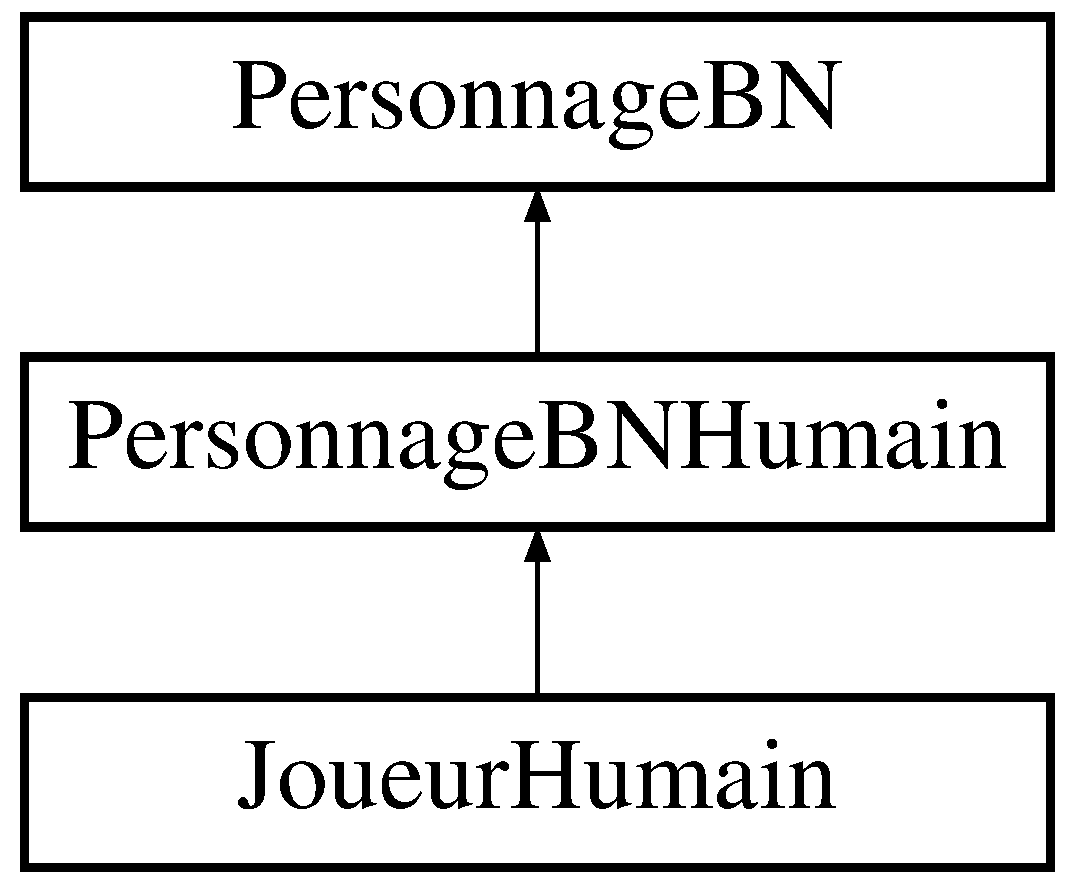
\includegraphics[height=3.000000cm]{classPersonnageBNHumain}
\end{center}
\end{figure}
\subsection*{Public Member Functions}
\begin{DoxyCompactItemize}
\item 
\hyperlink{classPersonnageBNHumain_a5d6c647bf6993595f2df0f557696a4f0}{Personnage\-B\-N\-Humain} (string nomnv)
\begin{DoxyCompactList}\small\item\em Constructeur des perso\-B\-N\-Humain. \end{DoxyCompactList}\item 
\hyperlink{classPersonnageBNHumain_a665cc1cafbcfda21103442ab8405c8d4}{Personnage\-B\-N\-Humain} (string nomnv, int l, int h, \hyperlink{classArme}{Arme} $\ast$a)
\begin{DoxyCompactList}\small\item\em Constructeur (très) parametre de personnage\-B\-N\-Humain. \end{DoxyCompactList}\item 
\hyperlink{classPersonnageBNHumain_a01247437df040f343c1ab9570e857664}{Personnage\-B\-N\-Humain} (string nomnv, \hyperlink{classArme}{Arme} $\ast$a)
\begin{DoxyCompactList}\small\item\em Constructeur (très) parametre de personnage\-B\-N\-Humain. \end{DoxyCompactList}\item 
\hyperlink{classPersonnageBNHumain_accecdded5770352d48561e6da60cf886}{Personnage\-B\-N\-Humain} (string nomnv, int l, int h)
\begin{DoxyCompactList}\small\item\em Constructeur (très) parametre de personnage\-B\-N\-Humain. \end{DoxyCompactList}\item 
\hyperlink{classPersonnageBNHumain_a489f81be78156eb0cf0493a78d3545d8}{Personnage\-B\-N\-Humain} (string nomnv, vector$<$ int $>$ t\-Bateaux)
\begin{DoxyCompactList}\small\item\em Constructeur des perso\-B\-N\-Humain. \end{DoxyCompactList}\item 
\hyperlink{classPersonnageBNHumain_aacdcaed63e62521aeed7aadfdf8b0e7d}{Personnage\-B\-N\-Humain} (string nomnv, int l, int h, vector$<$ int $>$ t\-Bateaux, \hyperlink{classArme}{Arme} $\ast$a)
\begin{DoxyCompactList}\small\item\em Constructeur (très) parametre de personnage\-B\-N\-Humain. \end{DoxyCompactList}\item 
\hyperlink{classPersonnageBNHumain_aff8b2756888d11ae5fffec2a9158bad0}{Personnage\-B\-N\-Humain} (string nomnv, vector$<$ int $>$ t\-Bateaux, \hyperlink{classArme}{Arme} $\ast$a)
\begin{DoxyCompactList}\small\item\em Constructeur (très) parametre de personnage\-B\-N\-Humain. \end{DoxyCompactList}\item 
\hyperlink{classPersonnageBNHumain_a8fb4350044fc697f253d72e0893155fb}{Personnage\-B\-N\-Humain} (string nomnv, int l, int h, vector$<$ int $>$ t\-Bateaux)
\begin{DoxyCompactList}\small\item\em Constructeur (très) parametre de personnage\-B\-N\-Humain. \end{DoxyCompactList}\item 
\hyperlink{classGrille}{Grille} \hyperlink{classPersonnageBNHumain_a66b59496aa63d4bc89183f600fa7f5df}{placer\-Bateaux} ()
\begin{DoxyCompactList}\small\item\em Place les bateaux. \end{DoxyCompactList}\item 
\hyperlink{classCoordonnees}{Coordonnees} \hyperlink{classPersonnageBNHumain_a31e1a81b570fe5aa77122b1b8beabb2e}{coordonnees\-A\-Viser} (\hyperlink{classGrille}{Grille} $\ast$grille\-Adverse)
\begin{DoxyCompactList}\small\item\em Attaque du P\-N\-J. \end{DoxyCompactList}\end{DoxyCompactItemize}


\subsection{Detailed Description}
\hyperlink{classPersonnage}{Personnage} de bataille navale associé au joueur. 

Cette classe contient les informations sur le personnage de bataille navale associé au joueur 

\subsection{Constructor \& Destructor Documentation}
\hypertarget{classPersonnageBNHumain_a5d6c647bf6993595f2df0f557696a4f0}{\index{Personnage\-B\-N\-Humain@{Personnage\-B\-N\-Humain}!Personnage\-B\-N\-Humain@{Personnage\-B\-N\-Humain}}
\index{Personnage\-B\-N\-Humain@{Personnage\-B\-N\-Humain}!PersonnageBNHumain@{Personnage\-B\-N\-Humain}}
\subsubsection[{Personnage\-B\-N\-Humain}]{\setlength{\rightskip}{0pt plus 5cm}Personnage\-B\-N\-Humain\-::\-Personnage\-B\-N\-Humain (
\begin{DoxyParamCaption}
\item[{string}]{nomnv}
\end{DoxyParamCaption}
)}}\label{classPersonnageBNHumain_a5d6c647bf6993595f2df0f557696a4f0}


Constructeur des perso\-B\-N\-Humain. 

Constructeur des perso\-B\-N\-Humain 
\begin{DoxyParams}{Parameters}
{\em nomnv} & \-: nom du joueur \\
\hline
\end{DoxyParams}
\hypertarget{classPersonnageBNHumain_a665cc1cafbcfda21103442ab8405c8d4}{\index{Personnage\-B\-N\-Humain@{Personnage\-B\-N\-Humain}!Personnage\-B\-N\-Humain@{Personnage\-B\-N\-Humain}}
\index{Personnage\-B\-N\-Humain@{Personnage\-B\-N\-Humain}!PersonnageBNHumain@{Personnage\-B\-N\-Humain}}
\subsubsection[{Personnage\-B\-N\-Humain}]{\setlength{\rightskip}{0pt plus 5cm}Personnage\-B\-N\-Humain\-::\-Personnage\-B\-N\-Humain (
\begin{DoxyParamCaption}
\item[{string}]{nomnv, }
\item[{int}]{l, }
\item[{int}]{h, }
\item[{{\bf Arme} $\ast$}]{a}
\end{DoxyParamCaption}
)}}\label{classPersonnageBNHumain_a665cc1cafbcfda21103442ab8405c8d4}


Constructeur (très) parametre de personnage\-B\-N\-Humain. 


\begin{DoxyParams}{Parameters}
{\em nomnv} & \-: nom du personnage \\
\hline
{\em l} & \-: longueur de la grille \\
\hline
{\em h} & \-: hauteur de la grille \\
\hline
{\em a} & \-: pointeur sur l'arme souhaitée \\
\hline
\end{DoxyParams}
\hypertarget{classPersonnageBNHumain_a01247437df040f343c1ab9570e857664}{\index{Personnage\-B\-N\-Humain@{Personnage\-B\-N\-Humain}!Personnage\-B\-N\-Humain@{Personnage\-B\-N\-Humain}}
\index{Personnage\-B\-N\-Humain@{Personnage\-B\-N\-Humain}!PersonnageBNHumain@{Personnage\-B\-N\-Humain}}
\subsubsection[{Personnage\-B\-N\-Humain}]{\setlength{\rightskip}{0pt plus 5cm}Personnage\-B\-N\-Humain\-::\-Personnage\-B\-N\-Humain (
\begin{DoxyParamCaption}
\item[{string}]{nomnv, }
\item[{{\bf Arme} $\ast$}]{a}
\end{DoxyParamCaption}
)}}\label{classPersonnageBNHumain_a01247437df040f343c1ab9570e857664}


Constructeur (très) parametre de personnage\-B\-N\-Humain. 


\begin{DoxyParams}{Parameters}
{\em nomnv} & \-: nom du personnage \\
\hline
{\em a} & \-: pointeur sur l'arme souhaitée \\
\hline
\end{DoxyParams}
\hypertarget{classPersonnageBNHumain_accecdded5770352d48561e6da60cf886}{\index{Personnage\-B\-N\-Humain@{Personnage\-B\-N\-Humain}!Personnage\-B\-N\-Humain@{Personnage\-B\-N\-Humain}}
\index{Personnage\-B\-N\-Humain@{Personnage\-B\-N\-Humain}!PersonnageBNHumain@{Personnage\-B\-N\-Humain}}
\subsubsection[{Personnage\-B\-N\-Humain}]{\setlength{\rightskip}{0pt plus 5cm}Personnage\-B\-N\-Humain\-::\-Personnage\-B\-N\-Humain (
\begin{DoxyParamCaption}
\item[{string}]{nomnv, }
\item[{int}]{l, }
\item[{int}]{h}
\end{DoxyParamCaption}
)}}\label{classPersonnageBNHumain_accecdded5770352d48561e6da60cf886}


Constructeur (très) parametre de personnage\-B\-N\-Humain. 


\begin{DoxyParams}{Parameters}
{\em nomnv} & \-: nom du personnage \\
\hline
{\em l} & \-: longueur de la grille \\
\hline
{\em h} & \-: hauteur de la grille \\
\hline
\end{DoxyParams}
\hypertarget{classPersonnageBNHumain_a489f81be78156eb0cf0493a78d3545d8}{\index{Personnage\-B\-N\-Humain@{Personnage\-B\-N\-Humain}!Personnage\-B\-N\-Humain@{Personnage\-B\-N\-Humain}}
\index{Personnage\-B\-N\-Humain@{Personnage\-B\-N\-Humain}!PersonnageBNHumain@{Personnage\-B\-N\-Humain}}
\subsubsection[{Personnage\-B\-N\-Humain}]{\setlength{\rightskip}{0pt plus 5cm}Personnage\-B\-N\-Humain\-::\-Personnage\-B\-N\-Humain (
\begin{DoxyParamCaption}
\item[{string}]{nomnv, }
\item[{vector$<$ int $>$}]{t\-Bateaux}
\end{DoxyParamCaption}
)}}\label{classPersonnageBNHumain_a489f81be78156eb0cf0493a78d3545d8}


Constructeur des perso\-B\-N\-Humain. 

Constructeur des perso\-B\-N\-Humain 
\begin{DoxyParams}{Parameters}
{\em t\-Bateaux} & \-: vector de taille de bateaux \\
\hline
{\em nomnv} & \-: nom du joueur \\
\hline
\end{DoxyParams}
\hypertarget{classPersonnageBNHumain_aacdcaed63e62521aeed7aadfdf8b0e7d}{\index{Personnage\-B\-N\-Humain@{Personnage\-B\-N\-Humain}!Personnage\-B\-N\-Humain@{Personnage\-B\-N\-Humain}}
\index{Personnage\-B\-N\-Humain@{Personnage\-B\-N\-Humain}!PersonnageBNHumain@{Personnage\-B\-N\-Humain}}
\subsubsection[{Personnage\-B\-N\-Humain}]{\setlength{\rightskip}{0pt plus 5cm}Personnage\-B\-N\-Humain\-::\-Personnage\-B\-N\-Humain (
\begin{DoxyParamCaption}
\item[{string}]{nomnv, }
\item[{int}]{l, }
\item[{int}]{h, }
\item[{vector$<$ int $>$}]{t\-Bateaux, }
\item[{{\bf Arme} $\ast$}]{a}
\end{DoxyParamCaption}
)}}\label{classPersonnageBNHumain_aacdcaed63e62521aeed7aadfdf8b0e7d}


Constructeur (très) parametre de personnage\-B\-N\-Humain. 


\begin{DoxyParams}{Parameters}
{\em nomnv} & \-: nom du personnage \\
\hline
{\em t\-Bateaux} & \-: vector de taille de bateaux \\
\hline
{\em l} & \-: longueur de la grille \\
\hline
{\em h} & \-: hauteur de la grille \\
\hline
{\em a} & \-: pointeur sur l'arme souhaitée \\
\hline
\end{DoxyParams}
\hypertarget{classPersonnageBNHumain_aff8b2756888d11ae5fffec2a9158bad0}{\index{Personnage\-B\-N\-Humain@{Personnage\-B\-N\-Humain}!Personnage\-B\-N\-Humain@{Personnage\-B\-N\-Humain}}
\index{Personnage\-B\-N\-Humain@{Personnage\-B\-N\-Humain}!PersonnageBNHumain@{Personnage\-B\-N\-Humain}}
\subsubsection[{Personnage\-B\-N\-Humain}]{\setlength{\rightskip}{0pt plus 5cm}Personnage\-B\-N\-Humain\-::\-Personnage\-B\-N\-Humain (
\begin{DoxyParamCaption}
\item[{string}]{nomnv, }
\item[{vector$<$ int $>$}]{t\-Bateaux, }
\item[{{\bf Arme} $\ast$}]{a}
\end{DoxyParamCaption}
)}}\label{classPersonnageBNHumain_aff8b2756888d11ae5fffec2a9158bad0}


Constructeur (très) parametre de personnage\-B\-N\-Humain. 


\begin{DoxyParams}{Parameters}
{\em t\-Bateaux} & \-: vector de taille de bateaux \\
\hline
{\em nomnv} & \-: nom du personnage \\
\hline
{\em a} & \-: pointeur sur l'arme souhaitée \\
\hline
\end{DoxyParams}
\hypertarget{classPersonnageBNHumain_a8fb4350044fc697f253d72e0893155fb}{\index{Personnage\-B\-N\-Humain@{Personnage\-B\-N\-Humain}!Personnage\-B\-N\-Humain@{Personnage\-B\-N\-Humain}}
\index{Personnage\-B\-N\-Humain@{Personnage\-B\-N\-Humain}!PersonnageBNHumain@{Personnage\-B\-N\-Humain}}
\subsubsection[{Personnage\-B\-N\-Humain}]{\setlength{\rightskip}{0pt plus 5cm}Personnage\-B\-N\-Humain\-::\-Personnage\-B\-N\-Humain (
\begin{DoxyParamCaption}
\item[{string}]{nomnv, }
\item[{int}]{l, }
\item[{int}]{h, }
\item[{vector$<$ int $>$}]{t\-Bateaux}
\end{DoxyParamCaption}
)}}\label{classPersonnageBNHumain_a8fb4350044fc697f253d72e0893155fb}


Constructeur (très) parametre de personnage\-B\-N\-Humain. 


\begin{DoxyParams}{Parameters}
{\em nomnv} & \-: nom du personnage \\
\hline
{\em t\-Bateaux} & \-: vector de taille de bateaux \\
\hline
{\em l} & \-: longueur de la grille \\
\hline
{\em h} & \-: hauteur de la grille \\
\hline
\end{DoxyParams}


\subsection{Member Function Documentation}
\hypertarget{classPersonnageBNHumain_a31e1a81b570fe5aa77122b1b8beabb2e}{\index{Personnage\-B\-N\-Humain@{Personnage\-B\-N\-Humain}!coordonnees\-A\-Viser@{coordonnees\-A\-Viser}}
\index{coordonnees\-A\-Viser@{coordonnees\-A\-Viser}!PersonnageBNHumain@{Personnage\-B\-N\-Humain}}
\subsubsection[{coordonnees\-A\-Viser}]{\setlength{\rightskip}{0pt plus 5cm}{\bf Coordonnees} Personnage\-B\-N\-Humain\-::coordonnees\-A\-Viser (
\begin{DoxyParamCaption}
\item[{{\bf Grille} $\ast$}]{grille\-Adverse}
\end{DoxyParamCaption}
)\hspace{0.3cm}{\ttfamily [virtual]}}}\label{classPersonnageBNHumain_a31e1a81b570fe5aa77122b1b8beabb2e}


Attaque du P\-N\-J. 

Demande où le joueur souhaite attaquer 
\begin{DoxyParams}{Parameters}
{\em grille\-Adverse} & \-: grille de l'adversaire \\
\hline
\end{DoxyParams}
\begin{DoxyReturn}{Returns}
les coordonnées de la case à attaquer 
\end{DoxyReturn}


Implements \hyperlink{classPersonnageBN_aaf4e97d763adba22bc5a89b2537e6dbe}{Personnage\-B\-N}.

\hypertarget{classPersonnageBNHumain_a66b59496aa63d4bc89183f600fa7f5df}{\index{Personnage\-B\-N\-Humain@{Personnage\-B\-N\-Humain}!placer\-Bateaux@{placer\-Bateaux}}
\index{placer\-Bateaux@{placer\-Bateaux}!PersonnageBNHumain@{Personnage\-B\-N\-Humain}}
\subsubsection[{placer\-Bateaux}]{\setlength{\rightskip}{0pt plus 5cm}{\bf Grille} Personnage\-B\-N\-Humain\-::placer\-Bateaux (
\begin{DoxyParamCaption}
{}
\end{DoxyParamCaption}
)\hspace{0.3cm}{\ttfamily [virtual]}}}\label{classPersonnageBNHumain_a66b59496aa63d4bc89183f600fa7f5df}


Place les bateaux. 

Demande au joueur de placer ses bateaux \begin{DoxyReturn}{Returns}
une grille avec les bateaux placés 
\end{DoxyReturn}


Implements \hyperlink{classPersonnageBN_a72b5b94a8e06f39c608c7310d4785579}{Personnage\-B\-N}.



The documentation for this class was generated from the following files\-:\begin{DoxyCompactItemize}
\item 
/home/damien/\-Bureau/projetcpp\-\_\-gm42/source/src/\hyperlink{PersonnageBNHumain_8hpp}{Personnage\-B\-N\-Humain.\-hpp}\item 
/home/damien/\-Bureau/projetcpp\-\_\-gm42/source/src/Personnage\-B\-N\-Humain.\-cpp\end{DoxyCompactItemize}

\hypertarget{classPersonnageBNIA}{\section{Personnage\-B\-N\-I\-A Class Reference}
\label{classPersonnageBNIA}\index{Personnage\-B\-N\-I\-A@{Personnage\-B\-N\-I\-A}}
}


Personnages de bataille navale dotés d'une intelligence artificielle.  




{\ttfamily \#include $<$Personnage\-B\-N\-I\-A.\-hpp$>$}

Inheritance diagram for Personnage\-B\-N\-I\-A\-:\begin{figure}[H]
\begin{center}
\leavevmode
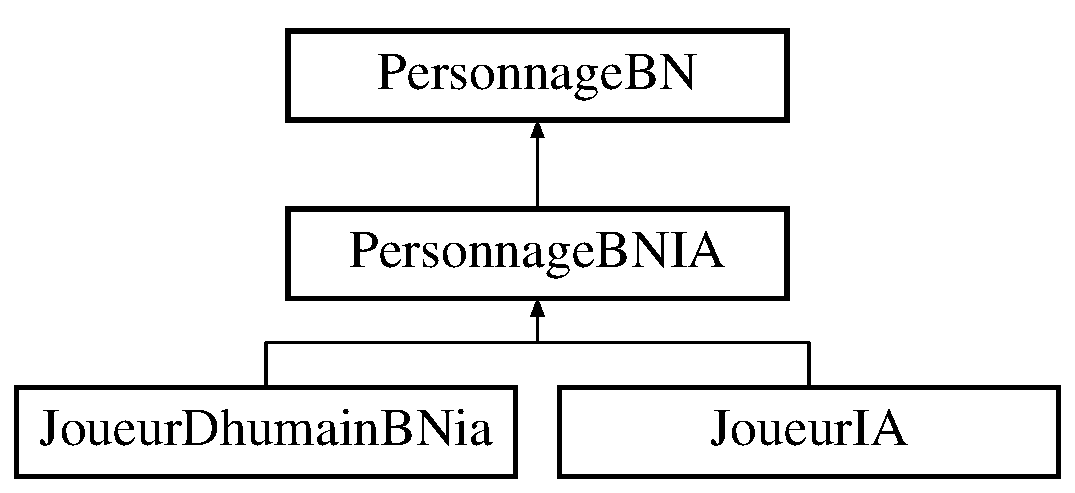
\includegraphics[height=3.000000cm]{classPersonnageBNIA}
\end{center}
\end{figure}
\subsection*{Public Member Functions}
\begin{DoxyCompactItemize}
\item 
\hyperlink{classPersonnageBNIA_a556e1751c26c06b8362a52ced1e59d46}{Personnage\-B\-N\-I\-A} (string nomnv)
\begin{DoxyCompactList}\small\item\em Constructeur des perso\-B\-N\-I\-A. \end{DoxyCompactList}\item 
\hyperlink{classPersonnageBNIA_a8eab753e71d557f78c0d66d92ff37b11}{Personnage\-B\-N\-I\-A} (string nomnv, int l, int h, \hyperlink{classArme}{Arme} $\ast$a)
\begin{DoxyCompactList}\small\item\em Constructeur (très) parametre de personnage\-B\-N\-I\-A. \end{DoxyCompactList}\item 
\hyperlink{classPersonnageBNIA_ab4e905ea8c6e7f6eab33337d77994eb9}{Personnage\-B\-N\-I\-A} (string nomnv, \hyperlink{classArme}{Arme} $\ast$a)
\begin{DoxyCompactList}\small\item\em Constructeur (très) parametre de personnage\-B\-N\-I\-A. \end{DoxyCompactList}\item 
\hyperlink{classPersonnageBNIA_a5dafceeaf4f7301be3f9c323d1c49fa6}{Personnage\-B\-N\-I\-A} (string nomnv, int l, int h)
\begin{DoxyCompactList}\small\item\em Constructeur (très) parametre de personnage\-B\-N\-I\-A. \end{DoxyCompactList}\item 
\hyperlink{classPersonnageBNIA_aa71da7518d1499bf69df71d7edff00b0}{Personnage\-B\-N\-I\-A} (string nomnv, vector$<$ int $>$ t\-Bateaux)
\begin{DoxyCompactList}\small\item\em Constructeur des perso\-B\-N\-I\-A. \end{DoxyCompactList}\item 
\hyperlink{classPersonnageBNIA_afc0183ca85ebcdce1bf714864e6a0dae}{Personnage\-B\-N\-I\-A} (string nomnv, int l, int h, vector$<$ int $>$ t\-Bateaux, \hyperlink{classArme}{Arme} $\ast$a)
\begin{DoxyCompactList}\small\item\em Constructeur (très) parametre de personnage\-B\-N\-I\-A. \end{DoxyCompactList}\item 
\hyperlink{classPersonnageBNIA_af887cba385ca100d46562435f0f28147}{Personnage\-B\-N\-I\-A} (string nomnv, vector$<$ int $>$ t\-Bateaux, \hyperlink{classArme}{Arme} $\ast$a)
\begin{DoxyCompactList}\small\item\em Constructeur (très) parametre de personnage\-B\-N\-I\-A. \end{DoxyCompactList}\item 
\hyperlink{classPersonnageBNIA_a2acba3f60a1e7c78674fd05370daa19b}{Personnage\-B\-N\-I\-A} (string nomnv, int l, int h, vector$<$ int $>$ t\-Bateaux)
\begin{DoxyCompactList}\small\item\em Constructeur (très) parametre de personnage\-B\-N\-I\-A. \end{DoxyCompactList}\item 
\hyperlink{classGrille}{Grille} \hyperlink{classPersonnageBNIA_ab9c5a33f853fb25c024ab12793256f88}{placer\-Bateaux} ()
\begin{DoxyCompactList}\small\item\em Place les bateaux. \end{DoxyCompactList}\item 
\hyperlink{classCoordonnees}{Coordonnees} \hyperlink{classPersonnageBNIA_a8a4246573cddf782fb4a0d9bcbd25832}{coordonnees\-A\-Viser} (\hyperlink{classGrille}{Grille} $\ast$grille\-Adverse)
\begin{DoxyCompactList}\small\item\em Attaque du P\-N\-J. \end{DoxyCompactList}\end{DoxyCompactItemize}


\subsection{Detailed Description}
Personnages de bataille navale dotés d'une intelligence artificielle. 

Cette classe contient les informations sur les personnages de bataille navale dotés d'une intelligence artificielle 

\subsection{Constructor \& Destructor Documentation}
\hypertarget{classPersonnageBNIA_a556e1751c26c06b8362a52ced1e59d46}{\index{Personnage\-B\-N\-I\-A@{Personnage\-B\-N\-I\-A}!Personnage\-B\-N\-I\-A@{Personnage\-B\-N\-I\-A}}
\index{Personnage\-B\-N\-I\-A@{Personnage\-B\-N\-I\-A}!PersonnageBNIA@{Personnage\-B\-N\-I\-A}}
\subsubsection[{Personnage\-B\-N\-I\-A}]{\setlength{\rightskip}{0pt plus 5cm}Personnage\-B\-N\-I\-A\-::\-Personnage\-B\-N\-I\-A (
\begin{DoxyParamCaption}
\item[{string}]{nomnv}
\end{DoxyParamCaption}
)}}\label{classPersonnageBNIA_a556e1751c26c06b8362a52ced1e59d46}


Constructeur des perso\-B\-N\-I\-A. 

Constructeur des perso\-B\-N\-I\-A 
\begin{DoxyParams}{Parameters}
{\em nomnv} & \-: nom du joueur \\
\hline
\end{DoxyParams}
\hypertarget{classPersonnageBNIA_a8eab753e71d557f78c0d66d92ff37b11}{\index{Personnage\-B\-N\-I\-A@{Personnage\-B\-N\-I\-A}!Personnage\-B\-N\-I\-A@{Personnage\-B\-N\-I\-A}}
\index{Personnage\-B\-N\-I\-A@{Personnage\-B\-N\-I\-A}!PersonnageBNIA@{Personnage\-B\-N\-I\-A}}
\subsubsection[{Personnage\-B\-N\-I\-A}]{\setlength{\rightskip}{0pt plus 5cm}Personnage\-B\-N\-I\-A\-::\-Personnage\-B\-N\-I\-A (
\begin{DoxyParamCaption}
\item[{string}]{nomnv, }
\item[{int}]{l, }
\item[{int}]{h, }
\item[{{\bf Arme} $\ast$}]{a}
\end{DoxyParamCaption}
)}}\label{classPersonnageBNIA_a8eab753e71d557f78c0d66d92ff37b11}


Constructeur (très) parametre de personnage\-B\-N\-I\-A. 


\begin{DoxyParams}{Parameters}
{\em nomnv} & \-: nom du personnage \\
\hline
{\em l} & \-: longueur de la grille \\
\hline
{\em h} & \-: hauteur de la grille \\
\hline
{\em a} & \-: pointeur sur l'arme souhaitée \\
\hline
\end{DoxyParams}
\hypertarget{classPersonnageBNIA_ab4e905ea8c6e7f6eab33337d77994eb9}{\index{Personnage\-B\-N\-I\-A@{Personnage\-B\-N\-I\-A}!Personnage\-B\-N\-I\-A@{Personnage\-B\-N\-I\-A}}
\index{Personnage\-B\-N\-I\-A@{Personnage\-B\-N\-I\-A}!PersonnageBNIA@{Personnage\-B\-N\-I\-A}}
\subsubsection[{Personnage\-B\-N\-I\-A}]{\setlength{\rightskip}{0pt plus 5cm}Personnage\-B\-N\-I\-A\-::\-Personnage\-B\-N\-I\-A (
\begin{DoxyParamCaption}
\item[{string}]{nomnv, }
\item[{{\bf Arme} $\ast$}]{a}
\end{DoxyParamCaption}
)}}\label{classPersonnageBNIA_ab4e905ea8c6e7f6eab33337d77994eb9}


Constructeur (très) parametre de personnage\-B\-N\-I\-A. 


\begin{DoxyParams}{Parameters}
{\em nomnv} & \-: nom du personnage \\
\hline
{\em a} & \-: pointeur sur l'arme souhaitée \\
\hline
\end{DoxyParams}
\hypertarget{classPersonnageBNIA_a5dafceeaf4f7301be3f9c323d1c49fa6}{\index{Personnage\-B\-N\-I\-A@{Personnage\-B\-N\-I\-A}!Personnage\-B\-N\-I\-A@{Personnage\-B\-N\-I\-A}}
\index{Personnage\-B\-N\-I\-A@{Personnage\-B\-N\-I\-A}!PersonnageBNIA@{Personnage\-B\-N\-I\-A}}
\subsubsection[{Personnage\-B\-N\-I\-A}]{\setlength{\rightskip}{0pt plus 5cm}Personnage\-B\-N\-I\-A\-::\-Personnage\-B\-N\-I\-A (
\begin{DoxyParamCaption}
\item[{string}]{nomnv, }
\item[{int}]{l, }
\item[{int}]{h}
\end{DoxyParamCaption}
)}}\label{classPersonnageBNIA_a5dafceeaf4f7301be3f9c323d1c49fa6}


Constructeur (très) parametre de personnage\-B\-N\-I\-A. 


\begin{DoxyParams}{Parameters}
{\em nomnv} & \-: nom du personnage \\
\hline
{\em l} & \-: longueur de la grille \\
\hline
{\em h} & \-: hauteur de la grille \\
\hline
\end{DoxyParams}
\hypertarget{classPersonnageBNIA_aa71da7518d1499bf69df71d7edff00b0}{\index{Personnage\-B\-N\-I\-A@{Personnage\-B\-N\-I\-A}!Personnage\-B\-N\-I\-A@{Personnage\-B\-N\-I\-A}}
\index{Personnage\-B\-N\-I\-A@{Personnage\-B\-N\-I\-A}!PersonnageBNIA@{Personnage\-B\-N\-I\-A}}
\subsubsection[{Personnage\-B\-N\-I\-A}]{\setlength{\rightskip}{0pt plus 5cm}Personnage\-B\-N\-I\-A\-::\-Personnage\-B\-N\-I\-A (
\begin{DoxyParamCaption}
\item[{string}]{nomnv, }
\item[{vector$<$ int $>$}]{t\-Bateaux}
\end{DoxyParamCaption}
)}}\label{classPersonnageBNIA_aa71da7518d1499bf69df71d7edff00b0}


Constructeur des perso\-B\-N\-I\-A. 

Constructeur des perso\-B\-N\-I\-A 
\begin{DoxyParams}{Parameters}
{\em t\-Bateaux} & \-: vector de taille de bateaux \\
\hline
{\em nomnv} & \-: nom du joueur \\
\hline
\end{DoxyParams}
\hypertarget{classPersonnageBNIA_afc0183ca85ebcdce1bf714864e6a0dae}{\index{Personnage\-B\-N\-I\-A@{Personnage\-B\-N\-I\-A}!Personnage\-B\-N\-I\-A@{Personnage\-B\-N\-I\-A}}
\index{Personnage\-B\-N\-I\-A@{Personnage\-B\-N\-I\-A}!PersonnageBNIA@{Personnage\-B\-N\-I\-A}}
\subsubsection[{Personnage\-B\-N\-I\-A}]{\setlength{\rightskip}{0pt plus 5cm}Personnage\-B\-N\-I\-A\-::\-Personnage\-B\-N\-I\-A (
\begin{DoxyParamCaption}
\item[{string}]{nomnv, }
\item[{int}]{l, }
\item[{int}]{h, }
\item[{vector$<$ int $>$}]{t\-Bateaux, }
\item[{{\bf Arme} $\ast$}]{a}
\end{DoxyParamCaption}
)}}\label{classPersonnageBNIA_afc0183ca85ebcdce1bf714864e6a0dae}


Constructeur (très) parametre de personnage\-B\-N\-I\-A. 


\begin{DoxyParams}{Parameters}
{\em nomnv} & \-: nom du personnage \\
\hline
{\em t\-Bateaux} & \-: vector de taille de bateaux \\
\hline
{\em l} & \-: longueur de la grille \\
\hline
{\em h} & \-: hauteur de la grille \\
\hline
{\em a} & \-: pointeur sur l'arme souhaitée \\
\hline
\end{DoxyParams}
\hypertarget{classPersonnageBNIA_af887cba385ca100d46562435f0f28147}{\index{Personnage\-B\-N\-I\-A@{Personnage\-B\-N\-I\-A}!Personnage\-B\-N\-I\-A@{Personnage\-B\-N\-I\-A}}
\index{Personnage\-B\-N\-I\-A@{Personnage\-B\-N\-I\-A}!PersonnageBNIA@{Personnage\-B\-N\-I\-A}}
\subsubsection[{Personnage\-B\-N\-I\-A}]{\setlength{\rightskip}{0pt plus 5cm}Personnage\-B\-N\-I\-A\-::\-Personnage\-B\-N\-I\-A (
\begin{DoxyParamCaption}
\item[{string}]{nomnv, }
\item[{vector$<$ int $>$}]{t\-Bateaux, }
\item[{{\bf Arme} $\ast$}]{a}
\end{DoxyParamCaption}
)}}\label{classPersonnageBNIA_af887cba385ca100d46562435f0f28147}


Constructeur (très) parametre de personnage\-B\-N\-I\-A. 


\begin{DoxyParams}{Parameters}
{\em t\-Bateaux} & \-: vector de taille de bateaux \\
\hline
{\em nomnv} & \-: nom du personnage \\
\hline
{\em a} & \-: pointeur sur l'arme souhaitée \\
\hline
\end{DoxyParams}
\hypertarget{classPersonnageBNIA_a2acba3f60a1e7c78674fd05370daa19b}{\index{Personnage\-B\-N\-I\-A@{Personnage\-B\-N\-I\-A}!Personnage\-B\-N\-I\-A@{Personnage\-B\-N\-I\-A}}
\index{Personnage\-B\-N\-I\-A@{Personnage\-B\-N\-I\-A}!PersonnageBNIA@{Personnage\-B\-N\-I\-A}}
\subsubsection[{Personnage\-B\-N\-I\-A}]{\setlength{\rightskip}{0pt plus 5cm}Personnage\-B\-N\-I\-A\-::\-Personnage\-B\-N\-I\-A (
\begin{DoxyParamCaption}
\item[{string}]{nomnv, }
\item[{int}]{l, }
\item[{int}]{h, }
\item[{vector$<$ int $>$}]{t\-Bateaux}
\end{DoxyParamCaption}
)}}\label{classPersonnageBNIA_a2acba3f60a1e7c78674fd05370daa19b}


Constructeur (très) parametre de personnage\-B\-N\-I\-A. 


\begin{DoxyParams}{Parameters}
{\em nomnv} & \-: nom du personnage \\
\hline
{\em t\-Bateaux} & \-: vector de taille de bateaux \\
\hline
{\em l} & \-: longueur de la grille \\
\hline
{\em h} & \-: hauteur de la grille \\
\hline
\end{DoxyParams}


\subsection{Member Function Documentation}
\hypertarget{classPersonnageBNIA_a8a4246573cddf782fb4a0d9bcbd25832}{\index{Personnage\-B\-N\-I\-A@{Personnage\-B\-N\-I\-A}!coordonnees\-A\-Viser@{coordonnees\-A\-Viser}}
\index{coordonnees\-A\-Viser@{coordonnees\-A\-Viser}!PersonnageBNIA@{Personnage\-B\-N\-I\-A}}
\subsubsection[{coordonnees\-A\-Viser}]{\setlength{\rightskip}{0pt plus 5cm}{\bf Coordonnees} Personnage\-B\-N\-I\-A\-::coordonnees\-A\-Viser (
\begin{DoxyParamCaption}
\item[{{\bf Grille} $\ast$}]{grille\-Adverse}
\end{DoxyParamCaption}
)\hspace{0.3cm}{\ttfamily [virtual]}}}\label{classPersonnageBNIA_a8a4246573cddf782fb4a0d9bcbd25832}


Attaque du P\-N\-J. 

Indique où le P\-N\-J attaque 
\begin{DoxyParams}{Parameters}
{\em grille\-Adverse} & \-: grille sur laquelle le joueur visr \\
\hline
\end{DoxyParams}
\begin{DoxyReturn}{Returns}
les coordonnées de la case à attaquer 
\end{DoxyReturn}


Implements \hyperlink{classPersonnageBN_aaf4e97d763adba22bc5a89b2537e6dbe}{Personnage\-B\-N}.

\hypertarget{classPersonnageBNIA_ab9c5a33f853fb25c024ab12793256f88}{\index{Personnage\-B\-N\-I\-A@{Personnage\-B\-N\-I\-A}!placer\-Bateaux@{placer\-Bateaux}}
\index{placer\-Bateaux@{placer\-Bateaux}!PersonnageBNIA@{Personnage\-B\-N\-I\-A}}
\subsubsection[{placer\-Bateaux}]{\setlength{\rightskip}{0pt plus 5cm}{\bf Grille} Personnage\-B\-N\-I\-A\-::placer\-Bateaux (
\begin{DoxyParamCaption}
{}
\end{DoxyParamCaption}
)\hspace{0.3cm}{\ttfamily [virtual]}}}\label{classPersonnageBNIA_ab9c5a33f853fb25c024ab12793256f88}


Place les bateaux. 

Place les bateaux de manière aléatoire \begin{DoxyReturn}{Returns}
une grille avec les bateaux placés 
\end{DoxyReturn}


Implements \hyperlink{classPersonnageBN_a72b5b94a8e06f39c608c7310d4785579}{Personnage\-B\-N}.



The documentation for this class was generated from the following files\-:\begin{DoxyCompactItemize}
\item 
/home/damien/\-Bureau/projetcpp\-\_\-gm42/source/src/\hyperlink{PersonnageBNIA_8hpp}{Personnage\-B\-N\-I\-A.\-hpp}\item 
/home/damien/\-Bureau/projetcpp\-\_\-gm42/source/src/Personnage\-B\-N\-I\-A.\-cpp\end{DoxyCompactItemize}

\hypertarget{classPersonnageBNIAAvance}{\section{Personnage\-B\-N\-I\-A\-Avance Class Reference}
\label{classPersonnageBNIAAvance}\index{Personnage\-B\-N\-I\-A\-Avance@{Personnage\-B\-N\-I\-A\-Avance}}
}


Personnages de bataille navale dotés d'une intelligence artificielle.  




{\ttfamily \#include $<$Personnage\-B\-N\-I\-A\-Avance.\-hpp$>$}

Inheritance diagram for Personnage\-B\-N\-I\-A\-Avance\-:\begin{figure}[H]
\begin{center}
\leavevmode
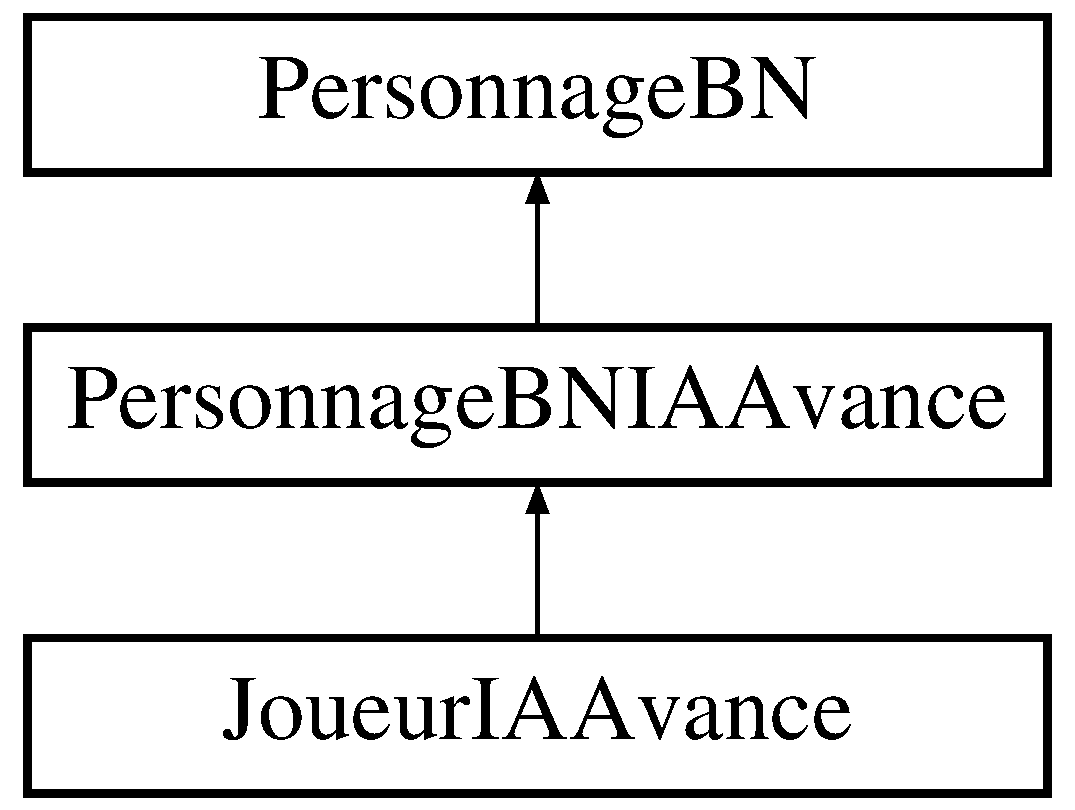
\includegraphics[height=3.000000cm]{classPersonnageBNIAAvance}
\end{center}
\end{figure}
\subsection*{Public Member Functions}
\begin{DoxyCompactItemize}
\item 
\hyperlink{classPersonnageBNIAAvance_a7d76f599d0e2f9aa12fe83e39376ec20}{Personnage\-B\-N\-I\-A\-Avance} (string nomnv)
\begin{DoxyCompactList}\small\item\em Constructeur des perso\-B\-N\-I\-A\-Avance. \end{DoxyCompactList}\item 
\hyperlink{classPersonnageBNIAAvance_a212d98b1b63d76ca0e16e3774a2787f8}{Personnage\-B\-N\-I\-A\-Avance} (string nomnv, int l, int h, \hyperlink{classArme}{Arme} $\ast$a)
\begin{DoxyCompactList}\small\item\em Constructeur (très) parametre de personnage\-B\-N\-I\-A\-Avance. \end{DoxyCompactList}\item 
\hyperlink{classPersonnageBNIAAvance_a8ec6b979b9154f6394e0e9c18c31c7cc}{Personnage\-B\-N\-I\-A\-Avance} (string nomnv, \hyperlink{classArme}{Arme} $\ast$a)
\begin{DoxyCompactList}\small\item\em Constructeur (très) parametre de personnage\-B\-N\-I\-A\-Avance. \end{DoxyCompactList}\item 
\hyperlink{classPersonnageBNIAAvance_aff9e64c9f9acc22463267487b8f12358}{Personnage\-B\-N\-I\-A\-Avance} (string nomnv, int l, int h)
\begin{DoxyCompactList}\small\item\em Constructeur (très) parametre de personnage\-B\-N\-I\-A\-Avance. \end{DoxyCompactList}\item 
\hyperlink{classPersonnageBNIAAvance_a789de7bfcd57dbff0675dd91f548bbab}{Personnage\-B\-N\-I\-A\-Avance} (string nomnv, vector$<$ int $>$ t\-Bateaux)
\begin{DoxyCompactList}\small\item\em Constructeur des perso\-B\-N\-I\-A\-Avance. \end{DoxyCompactList}\item 
\hyperlink{classPersonnageBNIAAvance_a50fad41761a1f1d36269cf264781ebe0}{Personnage\-B\-N\-I\-A\-Avance} (string nomnv, int l, int h, vector$<$ int $>$ t\-Bateaux, \hyperlink{classArme}{Arme} $\ast$a)
\begin{DoxyCompactList}\small\item\em Constructeur (très) parametre de personnage\-B\-N\-I\-A\-Avance. \end{DoxyCompactList}\item 
\hyperlink{classPersonnageBNIAAvance_a9d38388f7558508d80c54d47de851d1d}{Personnage\-B\-N\-I\-A\-Avance} (string nomnv, vector$<$ int $>$ t\-Bateaux, \hyperlink{classArme}{Arme} $\ast$a)
\begin{DoxyCompactList}\small\item\em Constructeur (très) parametre de personnage\-B\-N\-I\-A\-Avance. \end{DoxyCompactList}\item 
\hyperlink{classPersonnageBNIAAvance_a315fa9a64adcbcd808557461c6c8dbc4}{Personnage\-B\-N\-I\-A\-Avance} (string nomnv, int l, int h, vector$<$ int $>$ t\-Bateaux)
\begin{DoxyCompactList}\small\item\em Constructeur (très) parametre de personnage\-B\-N\-I\-A\-Avance. \end{DoxyCompactList}\item 
\hyperlink{classGrille}{Grille} \hyperlink{classPersonnageBNIAAvance_a9b6b532452a97556e50a9d44f19092f3}{placer\-Bateaux} ()
\begin{DoxyCompactList}\small\item\em Place les bateaux. \end{DoxyCompactList}\item 
\hyperlink{classCoordonnees}{Coordonnees} \hyperlink{classPersonnageBNIAAvance_a557435f197cea02489adc236c157f3ff}{tirer\-Aleatoirement} (\hyperlink{classGrille}{Grille} $\ast$grille\-Adverse)
\begin{DoxyCompactList}\small\item\em Attaque du P\-N\-J. \end{DoxyCompactList}\item 
\hyperlink{classCoordonnees}{Coordonnees} \hyperlink{classPersonnageBNIAAvance_a1927c24fe375190ad1d1f96a23c3e060}{coordonnees\-A\-Viser} (\hyperlink{classGrille}{Grille} $\ast$grille\-Adverse)
\begin{DoxyCompactList}\small\item\em Attaque du P\-N\-J lorsqu un bateau est touche. \end{DoxyCompactList}\end{DoxyCompactItemize}


\subsection{Detailed Description}
Personnages de bataille navale dotés d'une intelligence artificielle. 

Cette classe contient les informations sur les personnages de bataille navale dotés d'une intelligence artificielle 

\subsection{Constructor \& Destructor Documentation}
\hypertarget{classPersonnageBNIAAvance_a7d76f599d0e2f9aa12fe83e39376ec20}{\index{Personnage\-B\-N\-I\-A\-Avance@{Personnage\-B\-N\-I\-A\-Avance}!Personnage\-B\-N\-I\-A\-Avance@{Personnage\-B\-N\-I\-A\-Avance}}
\index{Personnage\-B\-N\-I\-A\-Avance@{Personnage\-B\-N\-I\-A\-Avance}!PersonnageBNIAAvance@{Personnage\-B\-N\-I\-A\-Avance}}
\subsubsection[{Personnage\-B\-N\-I\-A\-Avance}]{\setlength{\rightskip}{0pt plus 5cm}Personnage\-B\-N\-I\-A\-Avance\-::\-Personnage\-B\-N\-I\-A\-Avance (
\begin{DoxyParamCaption}
\item[{string}]{nomnv}
\end{DoxyParamCaption}
)}}\label{classPersonnageBNIAAvance_a7d76f599d0e2f9aa12fe83e39376ec20}


Constructeur des perso\-B\-N\-I\-A\-Avance. 

Constructeur des perso\-B\-N\-I\-A\-Avance 
\begin{DoxyParams}{Parameters}
{\em nomnv} & \-: nom du joueur \\
\hline
\end{DoxyParams}
\hypertarget{classPersonnageBNIAAvance_a212d98b1b63d76ca0e16e3774a2787f8}{\index{Personnage\-B\-N\-I\-A\-Avance@{Personnage\-B\-N\-I\-A\-Avance}!Personnage\-B\-N\-I\-A\-Avance@{Personnage\-B\-N\-I\-A\-Avance}}
\index{Personnage\-B\-N\-I\-A\-Avance@{Personnage\-B\-N\-I\-A\-Avance}!PersonnageBNIAAvance@{Personnage\-B\-N\-I\-A\-Avance}}
\subsubsection[{Personnage\-B\-N\-I\-A\-Avance}]{\setlength{\rightskip}{0pt plus 5cm}Personnage\-B\-N\-I\-A\-Avance\-::\-Personnage\-B\-N\-I\-A\-Avance (
\begin{DoxyParamCaption}
\item[{string}]{nomnv, }
\item[{int}]{l, }
\item[{int}]{h, }
\item[{{\bf Arme} $\ast$}]{a}
\end{DoxyParamCaption}
)}}\label{classPersonnageBNIAAvance_a212d98b1b63d76ca0e16e3774a2787f8}


Constructeur (très) parametre de personnage\-B\-N\-I\-A\-Avance. 


\begin{DoxyParams}{Parameters}
{\em nomnv} & \-: nom du personnage \\
\hline
{\em l} & \-: longueur de la grille \\
\hline
{\em h} & \-: hauteur de la grille \\
\hline
{\em a} & \-: pointeur sur l'arme souhaitée \\
\hline
\end{DoxyParams}
\hypertarget{classPersonnageBNIAAvance_a8ec6b979b9154f6394e0e9c18c31c7cc}{\index{Personnage\-B\-N\-I\-A\-Avance@{Personnage\-B\-N\-I\-A\-Avance}!Personnage\-B\-N\-I\-A\-Avance@{Personnage\-B\-N\-I\-A\-Avance}}
\index{Personnage\-B\-N\-I\-A\-Avance@{Personnage\-B\-N\-I\-A\-Avance}!PersonnageBNIAAvance@{Personnage\-B\-N\-I\-A\-Avance}}
\subsubsection[{Personnage\-B\-N\-I\-A\-Avance}]{\setlength{\rightskip}{0pt plus 5cm}Personnage\-B\-N\-I\-A\-Avance\-::\-Personnage\-B\-N\-I\-A\-Avance (
\begin{DoxyParamCaption}
\item[{string}]{nomnv, }
\item[{{\bf Arme} $\ast$}]{a}
\end{DoxyParamCaption}
)}}\label{classPersonnageBNIAAvance_a8ec6b979b9154f6394e0e9c18c31c7cc}


Constructeur (très) parametre de personnage\-B\-N\-I\-A\-Avance. 


\begin{DoxyParams}{Parameters}
{\em nomnv} & \-: nom du personnage \\
\hline
{\em a} & \-: pointeur sur l'arme souhaitée \\
\hline
\end{DoxyParams}
\hypertarget{classPersonnageBNIAAvance_aff9e64c9f9acc22463267487b8f12358}{\index{Personnage\-B\-N\-I\-A\-Avance@{Personnage\-B\-N\-I\-A\-Avance}!Personnage\-B\-N\-I\-A\-Avance@{Personnage\-B\-N\-I\-A\-Avance}}
\index{Personnage\-B\-N\-I\-A\-Avance@{Personnage\-B\-N\-I\-A\-Avance}!PersonnageBNIAAvance@{Personnage\-B\-N\-I\-A\-Avance}}
\subsubsection[{Personnage\-B\-N\-I\-A\-Avance}]{\setlength{\rightskip}{0pt plus 5cm}Personnage\-B\-N\-I\-A\-Avance\-::\-Personnage\-B\-N\-I\-A\-Avance (
\begin{DoxyParamCaption}
\item[{string}]{nomnv, }
\item[{int}]{l, }
\item[{int}]{h}
\end{DoxyParamCaption}
)}}\label{classPersonnageBNIAAvance_aff9e64c9f9acc22463267487b8f12358}


Constructeur (très) parametre de personnage\-B\-N\-I\-A\-Avance. 


\begin{DoxyParams}{Parameters}
{\em nomnv} & \-: nom du personnage \\
\hline
{\em l} & \-: longueur de la grille \\
\hline
{\em h} & \-: hauteur de la grille \\
\hline
\end{DoxyParams}
\hypertarget{classPersonnageBNIAAvance_a789de7bfcd57dbff0675dd91f548bbab}{\index{Personnage\-B\-N\-I\-A\-Avance@{Personnage\-B\-N\-I\-A\-Avance}!Personnage\-B\-N\-I\-A\-Avance@{Personnage\-B\-N\-I\-A\-Avance}}
\index{Personnage\-B\-N\-I\-A\-Avance@{Personnage\-B\-N\-I\-A\-Avance}!PersonnageBNIAAvance@{Personnage\-B\-N\-I\-A\-Avance}}
\subsubsection[{Personnage\-B\-N\-I\-A\-Avance}]{\setlength{\rightskip}{0pt plus 5cm}Personnage\-B\-N\-I\-A\-Avance\-::\-Personnage\-B\-N\-I\-A\-Avance (
\begin{DoxyParamCaption}
\item[{string}]{nomnv, }
\item[{vector$<$ int $>$}]{t\-Bateaux}
\end{DoxyParamCaption}
)}}\label{classPersonnageBNIAAvance_a789de7bfcd57dbff0675dd91f548bbab}


Constructeur des perso\-B\-N\-I\-A\-Avance. 

Constructeur des perso\-B\-N\-I\-A\-Avance 
\begin{DoxyParams}{Parameters}
{\em t\-Bateaux} & \-: vector de taille de bateaux \\
\hline
{\em nomnv} & \-: nom du joueur \\
\hline
\end{DoxyParams}
\hypertarget{classPersonnageBNIAAvance_a50fad41761a1f1d36269cf264781ebe0}{\index{Personnage\-B\-N\-I\-A\-Avance@{Personnage\-B\-N\-I\-A\-Avance}!Personnage\-B\-N\-I\-A\-Avance@{Personnage\-B\-N\-I\-A\-Avance}}
\index{Personnage\-B\-N\-I\-A\-Avance@{Personnage\-B\-N\-I\-A\-Avance}!PersonnageBNIAAvance@{Personnage\-B\-N\-I\-A\-Avance}}
\subsubsection[{Personnage\-B\-N\-I\-A\-Avance}]{\setlength{\rightskip}{0pt plus 5cm}Personnage\-B\-N\-I\-A\-Avance\-::\-Personnage\-B\-N\-I\-A\-Avance (
\begin{DoxyParamCaption}
\item[{string}]{nomnv, }
\item[{int}]{l, }
\item[{int}]{h, }
\item[{vector$<$ int $>$}]{t\-Bateaux, }
\item[{{\bf Arme} $\ast$}]{a}
\end{DoxyParamCaption}
)}}\label{classPersonnageBNIAAvance_a50fad41761a1f1d36269cf264781ebe0}


Constructeur (très) parametre de personnage\-B\-N\-I\-A\-Avance. 


\begin{DoxyParams}{Parameters}
{\em nomnv} & \-: nom du personnage \\
\hline
{\em t\-Bateaux} & \-: vector de taille de bateaux \\
\hline
{\em l} & \-: longueur de la grille \\
\hline
{\em h} & \-: hauteur de la grille \\
\hline
{\em a} & \-: pointeur sur l'arme souhaitée \\
\hline
\end{DoxyParams}
\hypertarget{classPersonnageBNIAAvance_a9d38388f7558508d80c54d47de851d1d}{\index{Personnage\-B\-N\-I\-A\-Avance@{Personnage\-B\-N\-I\-A\-Avance}!Personnage\-B\-N\-I\-A\-Avance@{Personnage\-B\-N\-I\-A\-Avance}}
\index{Personnage\-B\-N\-I\-A\-Avance@{Personnage\-B\-N\-I\-A\-Avance}!PersonnageBNIAAvance@{Personnage\-B\-N\-I\-A\-Avance}}
\subsubsection[{Personnage\-B\-N\-I\-A\-Avance}]{\setlength{\rightskip}{0pt plus 5cm}Personnage\-B\-N\-I\-A\-Avance\-::\-Personnage\-B\-N\-I\-A\-Avance (
\begin{DoxyParamCaption}
\item[{string}]{nomnv, }
\item[{vector$<$ int $>$}]{t\-Bateaux, }
\item[{{\bf Arme} $\ast$}]{a}
\end{DoxyParamCaption}
)}}\label{classPersonnageBNIAAvance_a9d38388f7558508d80c54d47de851d1d}


Constructeur (très) parametre de personnage\-B\-N\-I\-A\-Avance. 


\begin{DoxyParams}{Parameters}
{\em t\-Bateaux} & \-: vector de taille de bateaux \\
\hline
{\em nomnv} & \-: nom du personnage \\
\hline
{\em a} & \-: pointeur sur l'arme souhaitée \\
\hline
\end{DoxyParams}
\hypertarget{classPersonnageBNIAAvance_a315fa9a64adcbcd808557461c6c8dbc4}{\index{Personnage\-B\-N\-I\-A\-Avance@{Personnage\-B\-N\-I\-A\-Avance}!Personnage\-B\-N\-I\-A\-Avance@{Personnage\-B\-N\-I\-A\-Avance}}
\index{Personnage\-B\-N\-I\-A\-Avance@{Personnage\-B\-N\-I\-A\-Avance}!PersonnageBNIAAvance@{Personnage\-B\-N\-I\-A\-Avance}}
\subsubsection[{Personnage\-B\-N\-I\-A\-Avance}]{\setlength{\rightskip}{0pt plus 5cm}Personnage\-B\-N\-I\-A\-Avance\-::\-Personnage\-B\-N\-I\-A\-Avance (
\begin{DoxyParamCaption}
\item[{string}]{nomnv, }
\item[{int}]{l, }
\item[{int}]{h, }
\item[{vector$<$ int $>$}]{t\-Bateaux}
\end{DoxyParamCaption}
)}}\label{classPersonnageBNIAAvance_a315fa9a64adcbcd808557461c6c8dbc4}


Constructeur (très) parametre de personnage\-B\-N\-I\-A\-Avance. 


\begin{DoxyParams}{Parameters}
{\em nomnv} & \-: nom du personnage \\
\hline
{\em t\-Bateaux} & \-: vector de taille de bateaux \\
\hline
{\em l} & \-: longueur de la grille \\
\hline
{\em h} & \-: hauteur de la grille \\
\hline
\end{DoxyParams}


\subsection{Member Function Documentation}
\hypertarget{classPersonnageBNIAAvance_a1927c24fe375190ad1d1f96a23c3e060}{\index{Personnage\-B\-N\-I\-A\-Avance@{Personnage\-B\-N\-I\-A\-Avance}!coordonnees\-A\-Viser@{coordonnees\-A\-Viser}}
\index{coordonnees\-A\-Viser@{coordonnees\-A\-Viser}!PersonnageBNIAAvance@{Personnage\-B\-N\-I\-A\-Avance}}
\subsubsection[{coordonnees\-A\-Viser}]{\setlength{\rightskip}{0pt plus 5cm}{\bf Coordonnees} Personnage\-B\-N\-I\-A\-Avance\-::coordonnees\-A\-Viser (
\begin{DoxyParamCaption}
\item[{{\bf Grille} $\ast$}]{grille\-Adverse}
\end{DoxyParamCaption}
)\hspace{0.3cm}{\ttfamily [virtual]}}}\label{classPersonnageBNIAAvance_a1927c24fe375190ad1d1f96a23c3e060}


Attaque du P\-N\-J lorsqu un bateau est touche. 

Indique où le P\-N\-J attaque 
\begin{DoxyParams}{Parameters}
{\em grille\-Adverse} & \-: grille sur laquelle le joueur vise \\
\hline
\end{DoxyParams}
\begin{DoxyReturn}{Returns}
les coordonnees de la case à attaquer 
\end{DoxyReturn}


Implements \hyperlink{classPersonnageBN_aaf4e97d763adba22bc5a89b2537e6dbe}{Personnage\-B\-N}.

\hypertarget{classPersonnageBNIAAvance_a9b6b532452a97556e50a9d44f19092f3}{\index{Personnage\-B\-N\-I\-A\-Avance@{Personnage\-B\-N\-I\-A\-Avance}!placer\-Bateaux@{placer\-Bateaux}}
\index{placer\-Bateaux@{placer\-Bateaux}!PersonnageBNIAAvance@{Personnage\-B\-N\-I\-A\-Avance}}
\subsubsection[{placer\-Bateaux}]{\setlength{\rightskip}{0pt plus 5cm}{\bf Grille} Personnage\-B\-N\-I\-A\-Avance\-::placer\-Bateaux (
\begin{DoxyParamCaption}
{}
\end{DoxyParamCaption}
)\hspace{0.3cm}{\ttfamily [virtual]}}}\label{classPersonnageBNIAAvance_a9b6b532452a97556e50a9d44f19092f3}


Place les bateaux. 

Place les bateaux de manière aléatoire \begin{DoxyReturn}{Returns}
une grille avec les bateaux placés 
\end{DoxyReturn}


Implements \hyperlink{classPersonnageBN_a72b5b94a8e06f39c608c7310d4785579}{Personnage\-B\-N}.

\hypertarget{classPersonnageBNIAAvance_a557435f197cea02489adc236c157f3ff}{\index{Personnage\-B\-N\-I\-A\-Avance@{Personnage\-B\-N\-I\-A\-Avance}!tirer\-Aleatoirement@{tirer\-Aleatoirement}}
\index{tirer\-Aleatoirement@{tirer\-Aleatoirement}!PersonnageBNIAAvance@{Personnage\-B\-N\-I\-A\-Avance}}
\subsubsection[{tirer\-Aleatoirement}]{\setlength{\rightskip}{0pt plus 5cm}{\bf Coordonnees} Personnage\-B\-N\-I\-A\-Avance\-::tirer\-Aleatoirement (
\begin{DoxyParamCaption}
\item[{{\bf Grille} $\ast$}]{grille\-Adverse}
\end{DoxyParamCaption}
)}}\label{classPersonnageBNIAAvance_a557435f197cea02489adc236c157f3ff}


Attaque du P\-N\-J. 

Indique où le P\-N\-J attaque 
\begin{DoxyParams}{Parameters}
{\em grille\-Adverse} & \-: grille sur laquelle le joueur vise \\
\hline
\end{DoxyParams}
\begin{DoxyReturn}{Returns}
les coordonnées de la case à attaquer 
\end{DoxyReturn}


The documentation for this class was generated from the following files\-:\begin{DoxyCompactItemize}
\item 
/home/damien/\-Bureau/projetcpp\-\_\-gm42/source/src/\hyperlink{PersonnageBNIAAvance_8hpp}{Personnage\-B\-N\-I\-A\-Avance.\-hpp}\item 
/home/damien/\-Bureau/projetcpp\-\_\-gm42/source/src/Personnage\-B\-N\-I\-A\-Avance.\-cpp\end{DoxyCompactItemize}

\hypertarget{classPersonnageBNIACheate}{\section{Personnage\-B\-N\-I\-A\-Cheate Class Reference}
\label{classPersonnageBNIACheate}\index{Personnage\-B\-N\-I\-A\-Cheate@{Personnage\-B\-N\-I\-A\-Cheate}}
}


Personnages de bataille navale dotés d'une intelligence artificielle.  




{\ttfamily \#include $<$Personnage\-B\-N\-I\-A\-Cheate.\-hpp$>$}

Inheritance diagram for Personnage\-B\-N\-I\-A\-Cheate\-:\begin{figure}[H]
\begin{center}
\leavevmode
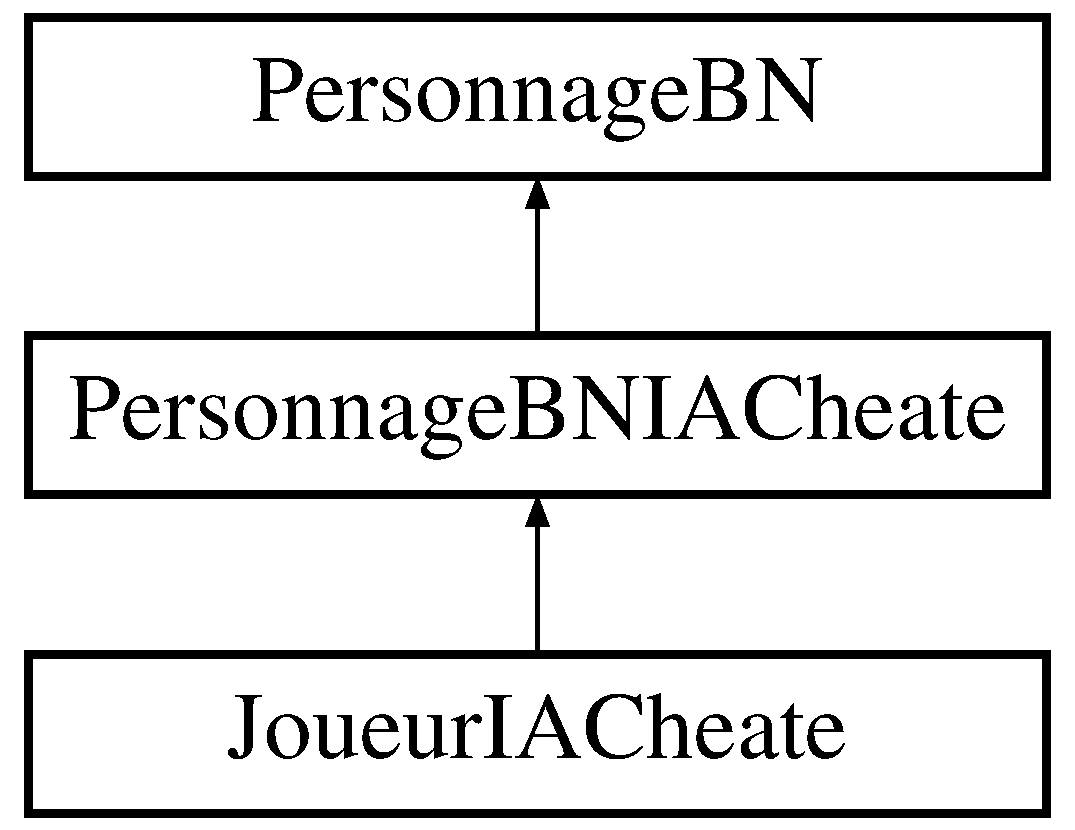
\includegraphics[height=3.000000cm]{classPersonnageBNIACheate}
\end{center}
\end{figure}
\subsection*{Public Member Functions}
\begin{DoxyCompactItemize}
\item 
\hyperlink{classPersonnageBNIACheate_a5327d1825c6b7df29b288f4d5d872dd1}{Personnage\-B\-N\-I\-A\-Cheate} (string nomnv)
\begin{DoxyCompactList}\small\item\em Constructeur des perso\-B\-N\-I\-A\-Cheate. \end{DoxyCompactList}\item 
\hyperlink{classPersonnageBNIACheate_a0a05adafe445a5883a688d99b0315274}{Personnage\-B\-N\-I\-A\-Cheate} (string nomnv, int l, int h, \hyperlink{classArme}{Arme} $\ast$a)
\begin{DoxyCompactList}\small\item\em Constructeur (très) parametre de personnage\-B\-N\-I\-A\-Cheate. \end{DoxyCompactList}\item 
\hyperlink{classPersonnageBNIACheate_ad5dbf2b4b3bf76e1d354f3e0bbf70517}{Personnage\-B\-N\-I\-A\-Cheate} (string nomnv, \hyperlink{classArme}{Arme} $\ast$a)
\begin{DoxyCompactList}\small\item\em Constructeur (très) parametre de personnage\-B\-N\-I\-A\-Cheate. \end{DoxyCompactList}\item 
\hyperlink{classPersonnageBNIACheate_a9177e565be9865898cb3b57df2550676}{Personnage\-B\-N\-I\-A\-Cheate} (string nomnv, int l, int h)
\begin{DoxyCompactList}\small\item\em Constructeur (très) parametre de personnage\-B\-N\-I\-A\-Cheate. \end{DoxyCompactList}\item 
\hyperlink{classPersonnageBNIACheate_a5d2bfdd856359c8344613d61af0deda8}{Personnage\-B\-N\-I\-A\-Cheate} (string nomnv, vector$<$ int $>$ t\-Bateaux)
\begin{DoxyCompactList}\small\item\em Constructeur des perso\-B\-N\-I\-A\-Cheate. \end{DoxyCompactList}\item 
\hyperlink{classPersonnageBNIACheate_ae3d3529526e4f3b021f215d96f1d3114}{Personnage\-B\-N\-I\-A\-Cheate} (string nomnv, int l, int h, vector$<$ int $>$ t\-Bateaux, \hyperlink{classArme}{Arme} $\ast$a)
\begin{DoxyCompactList}\small\item\em Constructeur (très) parametre de personnage\-B\-N\-I\-A\-Cheate. \end{DoxyCompactList}\item 
\hyperlink{classPersonnageBNIACheate_a11cfc16b65c677a73410fb46cc3ddd3a}{Personnage\-B\-N\-I\-A\-Cheate} (string nomnv, vector$<$ int $>$ t\-Bateaux, \hyperlink{classArme}{Arme} $\ast$a)
\begin{DoxyCompactList}\small\item\em Constructeur (très) parametre de personnage\-B\-N\-I\-A\-Cheate. \end{DoxyCompactList}\item 
\hyperlink{classPersonnageBNIACheate_ac663533e265cf49ff868b0eedb4de6a1}{Personnage\-B\-N\-I\-A\-Cheate} (string nomnv, int l, int h, vector$<$ int $>$ t\-Bateaux)
\begin{DoxyCompactList}\small\item\em Constructeur (très) parametre de personnage\-B\-N\-I\-A\-Cheate. \end{DoxyCompactList}\item 
\hyperlink{classGrille}{Grille} \hyperlink{classPersonnageBNIACheate_a76eabf30fe7ee8d8d00af7e4bac4cd3f}{placer\-Bateaux} ()
\begin{DoxyCompactList}\small\item\em Place les bateaux. \end{DoxyCompactList}\item 
\hyperlink{classCoordonnees}{Coordonnees} \hyperlink{classPersonnageBNIACheate_a7b81f85712b0f3d51427466b6fc4ebfd}{coordonnees\-A\-Viser} (\hyperlink{classGrille}{Grille} $\ast$grille\-Adverse)
\begin{DoxyCompactList}\small\item\em Attaque du P\-N\-J. \end{DoxyCompactList}\end{DoxyCompactItemize}


\subsection{Detailed Description}
Personnages de bataille navale dotés d'une intelligence artificielle. 

Cette classe contient les informations sur les personnages de bataille navale dotés d'une intelligence artificielle 

\subsection{Constructor \& Destructor Documentation}
\hypertarget{classPersonnageBNIACheate_a5327d1825c6b7df29b288f4d5d872dd1}{\index{Personnage\-B\-N\-I\-A\-Cheate@{Personnage\-B\-N\-I\-A\-Cheate}!Personnage\-B\-N\-I\-A\-Cheate@{Personnage\-B\-N\-I\-A\-Cheate}}
\index{Personnage\-B\-N\-I\-A\-Cheate@{Personnage\-B\-N\-I\-A\-Cheate}!PersonnageBNIACheate@{Personnage\-B\-N\-I\-A\-Cheate}}
\subsubsection[{Personnage\-B\-N\-I\-A\-Cheate}]{\setlength{\rightskip}{0pt plus 5cm}Personnage\-B\-N\-I\-A\-Cheate\-::\-Personnage\-B\-N\-I\-A\-Cheate (
\begin{DoxyParamCaption}
\item[{string}]{nomnv}
\end{DoxyParamCaption}
)}}\label{classPersonnageBNIACheate_a5327d1825c6b7df29b288f4d5d872dd1}


Constructeur des perso\-B\-N\-I\-A\-Cheate. 

Constructeur des perso\-B\-N\-I\-A\-Cheate 
\begin{DoxyParams}{Parameters}
{\em nomnv} & \-: nom du joueur \\
\hline
\end{DoxyParams}
\hypertarget{classPersonnageBNIACheate_a0a05adafe445a5883a688d99b0315274}{\index{Personnage\-B\-N\-I\-A\-Cheate@{Personnage\-B\-N\-I\-A\-Cheate}!Personnage\-B\-N\-I\-A\-Cheate@{Personnage\-B\-N\-I\-A\-Cheate}}
\index{Personnage\-B\-N\-I\-A\-Cheate@{Personnage\-B\-N\-I\-A\-Cheate}!PersonnageBNIACheate@{Personnage\-B\-N\-I\-A\-Cheate}}
\subsubsection[{Personnage\-B\-N\-I\-A\-Cheate}]{\setlength{\rightskip}{0pt plus 5cm}Personnage\-B\-N\-I\-A\-Cheate\-::\-Personnage\-B\-N\-I\-A\-Cheate (
\begin{DoxyParamCaption}
\item[{string}]{nomnv, }
\item[{int}]{l, }
\item[{int}]{h, }
\item[{{\bf Arme} $\ast$}]{a}
\end{DoxyParamCaption}
)}}\label{classPersonnageBNIACheate_a0a05adafe445a5883a688d99b0315274}


Constructeur (très) parametre de personnage\-B\-N\-I\-A\-Cheate. 


\begin{DoxyParams}{Parameters}
{\em nomnv} & \-: nom du personnage \\
\hline
{\em l} & \-: longueur de la grille \\
\hline
{\em h} & \-: hauteur de la grille \\
\hline
{\em a} & \-: pointeur sur l'arme souhaitée \\
\hline
\end{DoxyParams}
\hypertarget{classPersonnageBNIACheate_ad5dbf2b4b3bf76e1d354f3e0bbf70517}{\index{Personnage\-B\-N\-I\-A\-Cheate@{Personnage\-B\-N\-I\-A\-Cheate}!Personnage\-B\-N\-I\-A\-Cheate@{Personnage\-B\-N\-I\-A\-Cheate}}
\index{Personnage\-B\-N\-I\-A\-Cheate@{Personnage\-B\-N\-I\-A\-Cheate}!PersonnageBNIACheate@{Personnage\-B\-N\-I\-A\-Cheate}}
\subsubsection[{Personnage\-B\-N\-I\-A\-Cheate}]{\setlength{\rightskip}{0pt plus 5cm}Personnage\-B\-N\-I\-A\-Cheate\-::\-Personnage\-B\-N\-I\-A\-Cheate (
\begin{DoxyParamCaption}
\item[{string}]{nomnv, }
\item[{{\bf Arme} $\ast$}]{a}
\end{DoxyParamCaption}
)}}\label{classPersonnageBNIACheate_ad5dbf2b4b3bf76e1d354f3e0bbf70517}


Constructeur (très) parametre de personnage\-B\-N\-I\-A\-Cheate. 


\begin{DoxyParams}{Parameters}
{\em nomnv} & \-: nom du personnage \\
\hline
{\em a} & \-: pointeur sur l'arme souhaitée \\
\hline
\end{DoxyParams}
\hypertarget{classPersonnageBNIACheate_a9177e565be9865898cb3b57df2550676}{\index{Personnage\-B\-N\-I\-A\-Cheate@{Personnage\-B\-N\-I\-A\-Cheate}!Personnage\-B\-N\-I\-A\-Cheate@{Personnage\-B\-N\-I\-A\-Cheate}}
\index{Personnage\-B\-N\-I\-A\-Cheate@{Personnage\-B\-N\-I\-A\-Cheate}!PersonnageBNIACheate@{Personnage\-B\-N\-I\-A\-Cheate}}
\subsubsection[{Personnage\-B\-N\-I\-A\-Cheate}]{\setlength{\rightskip}{0pt plus 5cm}Personnage\-B\-N\-I\-A\-Cheate\-::\-Personnage\-B\-N\-I\-A\-Cheate (
\begin{DoxyParamCaption}
\item[{string}]{nomnv, }
\item[{int}]{l, }
\item[{int}]{h}
\end{DoxyParamCaption}
)}}\label{classPersonnageBNIACheate_a9177e565be9865898cb3b57df2550676}


Constructeur (très) parametre de personnage\-B\-N\-I\-A\-Cheate. 


\begin{DoxyParams}{Parameters}
{\em nomnv} & \-: nom du personnage \\
\hline
{\em l} & \-: longueur de la grille \\
\hline
{\em h} & \-: hauteur de la grille \\
\hline
\end{DoxyParams}
\hypertarget{classPersonnageBNIACheate_a5d2bfdd856359c8344613d61af0deda8}{\index{Personnage\-B\-N\-I\-A\-Cheate@{Personnage\-B\-N\-I\-A\-Cheate}!Personnage\-B\-N\-I\-A\-Cheate@{Personnage\-B\-N\-I\-A\-Cheate}}
\index{Personnage\-B\-N\-I\-A\-Cheate@{Personnage\-B\-N\-I\-A\-Cheate}!PersonnageBNIACheate@{Personnage\-B\-N\-I\-A\-Cheate}}
\subsubsection[{Personnage\-B\-N\-I\-A\-Cheate}]{\setlength{\rightskip}{0pt plus 5cm}Personnage\-B\-N\-I\-A\-Cheate\-::\-Personnage\-B\-N\-I\-A\-Cheate (
\begin{DoxyParamCaption}
\item[{string}]{nomnv, }
\item[{vector$<$ int $>$}]{t\-Bateaux}
\end{DoxyParamCaption}
)}}\label{classPersonnageBNIACheate_a5d2bfdd856359c8344613d61af0deda8}


Constructeur des perso\-B\-N\-I\-A\-Cheate. 

Constructeur des perso\-B\-N\-I\-A\-Cheate 
\begin{DoxyParams}{Parameters}
{\em t\-Bateaux} & \-: vector de taille de bateaux \\
\hline
{\em nomnv} & \-: nom du joueur \\
\hline
\end{DoxyParams}
\hypertarget{classPersonnageBNIACheate_ae3d3529526e4f3b021f215d96f1d3114}{\index{Personnage\-B\-N\-I\-A\-Cheate@{Personnage\-B\-N\-I\-A\-Cheate}!Personnage\-B\-N\-I\-A\-Cheate@{Personnage\-B\-N\-I\-A\-Cheate}}
\index{Personnage\-B\-N\-I\-A\-Cheate@{Personnage\-B\-N\-I\-A\-Cheate}!PersonnageBNIACheate@{Personnage\-B\-N\-I\-A\-Cheate}}
\subsubsection[{Personnage\-B\-N\-I\-A\-Cheate}]{\setlength{\rightskip}{0pt plus 5cm}Personnage\-B\-N\-I\-A\-Cheate\-::\-Personnage\-B\-N\-I\-A\-Cheate (
\begin{DoxyParamCaption}
\item[{string}]{nomnv, }
\item[{int}]{l, }
\item[{int}]{h, }
\item[{vector$<$ int $>$}]{t\-Bateaux, }
\item[{{\bf Arme} $\ast$}]{a}
\end{DoxyParamCaption}
)}}\label{classPersonnageBNIACheate_ae3d3529526e4f3b021f215d96f1d3114}


Constructeur (très) parametre de personnage\-B\-N\-I\-A\-Cheate. 


\begin{DoxyParams}{Parameters}
{\em nomnv} & \-: nom du personnage \\
\hline
{\em t\-Bateaux} & \-: vector de taille de bateaux \\
\hline
{\em l} & \-: longueur de la grille \\
\hline
{\em h} & \-: hauteur de la grille \\
\hline
{\em a} & \-: pointeur sur l'arme souhaitée \\
\hline
\end{DoxyParams}
\hypertarget{classPersonnageBNIACheate_a11cfc16b65c677a73410fb46cc3ddd3a}{\index{Personnage\-B\-N\-I\-A\-Cheate@{Personnage\-B\-N\-I\-A\-Cheate}!Personnage\-B\-N\-I\-A\-Cheate@{Personnage\-B\-N\-I\-A\-Cheate}}
\index{Personnage\-B\-N\-I\-A\-Cheate@{Personnage\-B\-N\-I\-A\-Cheate}!PersonnageBNIACheate@{Personnage\-B\-N\-I\-A\-Cheate}}
\subsubsection[{Personnage\-B\-N\-I\-A\-Cheate}]{\setlength{\rightskip}{0pt plus 5cm}Personnage\-B\-N\-I\-A\-Cheate\-::\-Personnage\-B\-N\-I\-A\-Cheate (
\begin{DoxyParamCaption}
\item[{string}]{nomnv, }
\item[{vector$<$ int $>$}]{t\-Bateaux, }
\item[{{\bf Arme} $\ast$}]{a}
\end{DoxyParamCaption}
)}}\label{classPersonnageBNIACheate_a11cfc16b65c677a73410fb46cc3ddd3a}


Constructeur (très) parametre de personnage\-B\-N\-I\-A\-Cheate. 


\begin{DoxyParams}{Parameters}
{\em t\-Bateaux} & \-: vector de taille de bateaux \\
\hline
{\em nomnv} & \-: nom du personnage \\
\hline
{\em a} & \-: pointeur sur l'arme souhaitée \\
\hline
\end{DoxyParams}
\hypertarget{classPersonnageBNIACheate_ac663533e265cf49ff868b0eedb4de6a1}{\index{Personnage\-B\-N\-I\-A\-Cheate@{Personnage\-B\-N\-I\-A\-Cheate}!Personnage\-B\-N\-I\-A\-Cheate@{Personnage\-B\-N\-I\-A\-Cheate}}
\index{Personnage\-B\-N\-I\-A\-Cheate@{Personnage\-B\-N\-I\-A\-Cheate}!PersonnageBNIACheate@{Personnage\-B\-N\-I\-A\-Cheate}}
\subsubsection[{Personnage\-B\-N\-I\-A\-Cheate}]{\setlength{\rightskip}{0pt plus 5cm}Personnage\-B\-N\-I\-A\-Cheate\-::\-Personnage\-B\-N\-I\-A\-Cheate (
\begin{DoxyParamCaption}
\item[{string}]{nomnv, }
\item[{int}]{l, }
\item[{int}]{h, }
\item[{vector$<$ int $>$}]{t\-Bateaux}
\end{DoxyParamCaption}
)}}\label{classPersonnageBNIACheate_ac663533e265cf49ff868b0eedb4de6a1}


Constructeur (très) parametre de personnage\-B\-N\-I\-A\-Cheate. 


\begin{DoxyParams}{Parameters}
{\em nomnv} & \-: nom du personnage \\
\hline
{\em t\-Bateaux} & \-: vector de taille de bateaux \\
\hline
{\em l} & \-: longueur de la grille \\
\hline
{\em h} & \-: hauteur de la grille \\
\hline
\end{DoxyParams}


\subsection{Member Function Documentation}
\hypertarget{classPersonnageBNIACheate_a7b81f85712b0f3d51427466b6fc4ebfd}{\index{Personnage\-B\-N\-I\-A\-Cheate@{Personnage\-B\-N\-I\-A\-Cheate}!coordonnees\-A\-Viser@{coordonnees\-A\-Viser}}
\index{coordonnees\-A\-Viser@{coordonnees\-A\-Viser}!PersonnageBNIACheate@{Personnage\-B\-N\-I\-A\-Cheate}}
\subsubsection[{coordonnees\-A\-Viser}]{\setlength{\rightskip}{0pt plus 5cm}{\bf Coordonnees} Personnage\-B\-N\-I\-A\-Cheate\-::coordonnees\-A\-Viser (
\begin{DoxyParamCaption}
\item[{{\bf Grille} $\ast$}]{grille\-Adverse}
\end{DoxyParamCaption}
)\hspace{0.3cm}{\ttfamily [virtual]}}}\label{classPersonnageBNIACheate_a7b81f85712b0f3d51427466b6fc4ebfd}


Attaque du P\-N\-J. 

Indique où le P\-N\-J attaque 
\begin{DoxyParams}{Parameters}
{\em grille\-Adverse} & \-: grille sur laquelle le joueur visr \\
\hline
\end{DoxyParams}
\begin{DoxyReturn}{Returns}
les coordonnées de la case à attaquer 
\end{DoxyReturn}


Implements \hyperlink{classPersonnageBN_aaf4e97d763adba22bc5a89b2537e6dbe}{Personnage\-B\-N}.

\hypertarget{classPersonnageBNIACheate_a76eabf30fe7ee8d8d00af7e4bac4cd3f}{\index{Personnage\-B\-N\-I\-A\-Cheate@{Personnage\-B\-N\-I\-A\-Cheate}!placer\-Bateaux@{placer\-Bateaux}}
\index{placer\-Bateaux@{placer\-Bateaux}!PersonnageBNIACheate@{Personnage\-B\-N\-I\-A\-Cheate}}
\subsubsection[{placer\-Bateaux}]{\setlength{\rightskip}{0pt plus 5cm}{\bf Grille} Personnage\-B\-N\-I\-A\-Cheate\-::placer\-Bateaux (
\begin{DoxyParamCaption}
{}
\end{DoxyParamCaption}
)\hspace{0.3cm}{\ttfamily [virtual]}}}\label{classPersonnageBNIACheate_a76eabf30fe7ee8d8d00af7e4bac4cd3f}


Place les bateaux. 

Place les bateaux de manière aléatoire \begin{DoxyReturn}{Returns}
une grille avec les bateaux placés 
\end{DoxyReturn}


Implements \hyperlink{classPersonnageBN_a72b5b94a8e06f39c608c7310d4785579}{Personnage\-B\-N}.



The documentation for this class was generated from the following files\-:\begin{DoxyCompactItemize}
\item 
/home/damien/\-Bureau/projetcpp\-\_\-gm42/source/src/\hyperlink{PersonnageBNIACheate_8hpp}{Personnage\-B\-N\-I\-A\-Cheate.\-hpp}\item 
/home/damien/\-Bureau/projetcpp\-\_\-gm42/source/src/Personnage\-B\-N\-I\-A\-Cheate.\-cpp\end{DoxyCompactItemize}

\hypertarget{classPersonnageJouable}{\section{Personnage\-Jouable Class Reference}
\label{classPersonnageJouable}\index{Personnage\-Jouable@{Personnage\-Jouable}}
}


classe definissant un personnage jouable  




{\ttfamily \#include $<$Personnage\-Jouable.\-hpp$>$}

Inheritance diagram for Personnage\-Jouable\-:\begin{figure}[H]
\begin{center}
\leavevmode
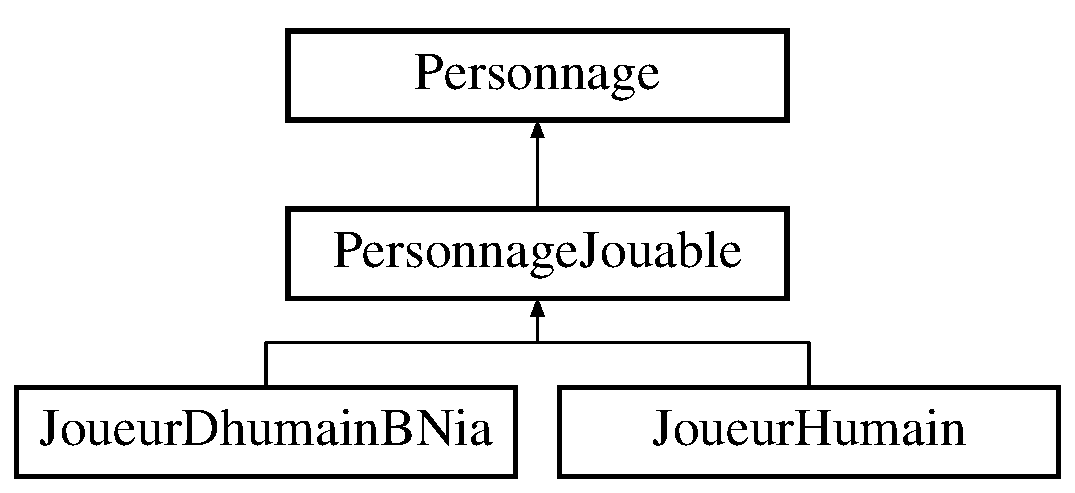
\includegraphics[height=3.000000cm]{classPersonnageJouable}
\end{center}
\end{figure}
\subsection*{Public Member Functions}
\begin{DoxyCompactItemize}
\item 
\hyperlink{classPersonnageJouable_a140604ca5b0fe1e38dd556ee3045f3cb}{Personnage\-Jouable} (string nomnv, \hyperlink{classCoordonnees}{Coordonnees} coord, \hyperlink{classCarte}{Carte} $\ast$id\-Carte)
\begin{DoxyCompactList}\small\item\em constructeur \end{DoxyCompactList}\item 
\hyperlink{classPersonnageJouable_a1bbbb6e3a1849dc226b8c2ab4bfa969c}{Personnage\-Jouable} (string nomnv)
\begin{DoxyCompactList}\small\item\em constructeur \end{DoxyCompactList}\item 
\hypertarget{classPersonnageJouable_a1ae6ed8c67f573a386ecd8b44c46c978}{void \hyperlink{classPersonnageJouable_a1ae6ed8c67f573a386ecd8b44c46c978}{deplacement\-Initial} ()}\label{classPersonnageJouable_a1ae6ed8c67f573a386ecd8b44c46c978}

\begin{DoxyCompactList}\small\item\em Remet le personnage à son emplacement initial. \end{DoxyCompactList}\item 
\hyperlink{classCarte}{Carte} $\ast$ \hyperlink{classPersonnageJouable_a9ba5eaf18bd33150acc3f042d34deb84}{get\-Id\-Carte\-Init} () const 
\begin{DoxyCompactList}\small\item\em getter \end{DoxyCompactList}\item 
\hyperlink{classCoordonnees}{Coordonnees} \hyperlink{classPersonnageJouable_a9ad36be16bae232f9c33478374143832}{get\-Coordonnees\-Init} () const 
\begin{DoxyCompactList}\small\item\em getter \end{DoxyCompactList}\end{DoxyCompactItemize}


\subsection{Detailed Description}
classe definissant un personnage jouable 

La classe représente un personnage jouable 

\subsection{Constructor \& Destructor Documentation}
\hypertarget{classPersonnageJouable_a140604ca5b0fe1e38dd556ee3045f3cb}{\index{Personnage\-Jouable@{Personnage\-Jouable}!Personnage\-Jouable@{Personnage\-Jouable}}
\index{Personnage\-Jouable@{Personnage\-Jouable}!PersonnageJouable@{Personnage\-Jouable}}
\subsubsection[{Personnage\-Jouable}]{\setlength{\rightskip}{0pt plus 5cm}Personnage\-Jouable\-::\-Personnage\-Jouable (
\begin{DoxyParamCaption}
\item[{string}]{nomnv, }
\item[{{\bf Coordonnees}}]{coord, }
\item[{{\bf Carte} $\ast$}]{id\-Carte}
\end{DoxyParamCaption}
)}}\label{classPersonnageJouable_a140604ca5b0fe1e38dd556ee3045f3cb}


constructeur 


\begin{DoxyParams}{Parameters}
{\em nomnv} & \-: nom du joueur \\
\hline
{\em coord} & \-: coordonnees du joueur \\
\hline
{\em id\-Carte} & \-: pointeur sur carte où se trouve le joueur \\
\hline
\end{DoxyParams}
\hypertarget{classPersonnageJouable_a1bbbb6e3a1849dc226b8c2ab4bfa969c}{\index{Personnage\-Jouable@{Personnage\-Jouable}!Personnage\-Jouable@{Personnage\-Jouable}}
\index{Personnage\-Jouable@{Personnage\-Jouable}!PersonnageJouable@{Personnage\-Jouable}}
\subsubsection[{Personnage\-Jouable}]{\setlength{\rightskip}{0pt plus 5cm}Personnage\-Jouable\-::\-Personnage\-Jouable (
\begin{DoxyParamCaption}
\item[{string}]{nomnv}
\end{DoxyParamCaption}
)}}\label{classPersonnageJouable_a1bbbb6e3a1849dc226b8c2ab4bfa969c}


constructeur 


\begin{DoxyParams}{Parameters}
{\em nomnv} & \-: nom du joueur \\
\hline
\end{DoxyParams}


\subsection{Member Function Documentation}
\hypertarget{classPersonnageJouable_a9ad36be16bae232f9c33478374143832}{\index{Personnage\-Jouable@{Personnage\-Jouable}!get\-Coordonnees\-Init@{get\-Coordonnees\-Init}}
\index{get\-Coordonnees\-Init@{get\-Coordonnees\-Init}!PersonnageJouable@{Personnage\-Jouable}}
\subsubsection[{get\-Coordonnees\-Init}]{\setlength{\rightskip}{0pt plus 5cm}{\bf Coordonnees} Personnage\-Jouable\-::get\-Coordonnees\-Init (
\begin{DoxyParamCaption}
{}
\end{DoxyParamCaption}
) const}}\label{classPersonnageJouable_a9ad36be16bae232f9c33478374143832}


getter 

\begin{DoxyReturn}{Returns}
\hyperlink{classCoordonnees}{Coordonnees} 
\end{DoxyReturn}
\hypertarget{classPersonnageJouable_a9ba5eaf18bd33150acc3f042d34deb84}{\index{Personnage\-Jouable@{Personnage\-Jouable}!get\-Id\-Carte\-Init@{get\-Id\-Carte\-Init}}
\index{get\-Id\-Carte\-Init@{get\-Id\-Carte\-Init}!PersonnageJouable@{Personnage\-Jouable}}
\subsubsection[{get\-Id\-Carte\-Init}]{\setlength{\rightskip}{0pt plus 5cm}{\bf Carte} $\ast$ Personnage\-Jouable\-::get\-Id\-Carte\-Init (
\begin{DoxyParamCaption}
{}
\end{DoxyParamCaption}
) const}}\label{classPersonnageJouable_a9ba5eaf18bd33150acc3f042d34deb84}


getter 

\begin{DoxyReturn}{Returns}
\hyperlink{classCarte}{Carte} 
\end{DoxyReturn}


The documentation for this class was generated from the following files\-:\begin{DoxyCompactItemize}
\item 
/home/damien/\-Bureau/projetcpp\-\_\-gm42/source/src/\hyperlink{PersonnageJouable_8hpp}{Personnage\-Jouable.\-hpp}\item 
/home/damien/\-Bureau/projetcpp\-\_\-gm42/source/src/Personnage\-Jouable.\-cpp\end{DoxyCompactItemize}

\hypertarget{classPersonnageNonJouable}{\section{Personnage\-Non\-Jouable Class Reference}
\label{classPersonnageNonJouable}\index{Personnage\-Non\-Jouable@{Personnage\-Non\-Jouable}}
}


classe définissant un personnage non jouable  




{\ttfamily \#include $<$Personnage\-Non\-Jouable.\-hpp$>$}

Inheritance diagram for Personnage\-Non\-Jouable\-:\begin{figure}[H]
\begin{center}
\leavevmode
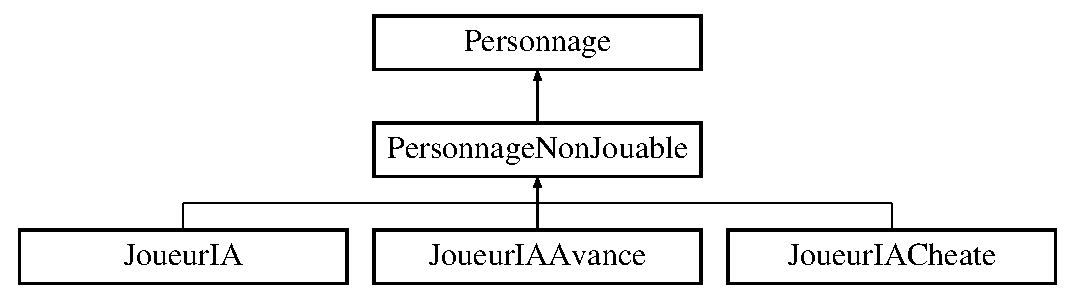
\includegraphics[height=3.000000cm]{classPersonnageNonJouable}
\end{center}
\end{figure}
\subsection*{Public Member Functions}
\begin{DoxyCompactItemize}
\item 
\hyperlink{classPersonnageNonJouable_ac647e57fa08d14e0ce334702bdbe38f1}{Personnage\-Non\-Jouable} (string nomnv)
\begin{DoxyCompactList}\small\item\em constructeur de P\-N\-J \end{DoxyCompactList}\end{DoxyCompactItemize}


\subsection{Detailed Description}
classe définissant un personnage non jouable 

La classe représente un personnage non jouable 

\subsection{Constructor \& Destructor Documentation}
\hypertarget{classPersonnageNonJouable_ac647e57fa08d14e0ce334702bdbe38f1}{\index{Personnage\-Non\-Jouable@{Personnage\-Non\-Jouable}!Personnage\-Non\-Jouable@{Personnage\-Non\-Jouable}}
\index{Personnage\-Non\-Jouable@{Personnage\-Non\-Jouable}!PersonnageNonJouable@{Personnage\-Non\-Jouable}}
\subsubsection[{Personnage\-Non\-Jouable}]{\setlength{\rightskip}{0pt plus 5cm}Personnage\-Non\-Jouable\-::\-Personnage\-Non\-Jouable (
\begin{DoxyParamCaption}
\item[{string}]{nomnv}
\end{DoxyParamCaption}
)}}\label{classPersonnageNonJouable_ac647e57fa08d14e0ce334702bdbe38f1}


constructeur de P\-N\-J 


\begin{DoxyParams}{Parameters}
{\em nomnv} & nom du personnage \\
\hline
\end{DoxyParams}


The documentation for this class was generated from the following files\-:\begin{DoxyCompactItemize}
\item 
/home/damien/\-Bureau/projetcpp\-\_\-gm42/source/src/\hyperlink{PersonnageNonJouable_8hpp}{Personnage\-Non\-Jouable.\-hpp}\item 
/home/damien/\-Bureau/projetcpp\-\_\-gm42/source/src/Personnage\-Non\-Jouable.\-cpp\end{DoxyCompactItemize}

\hypertarget{classTailleGrille}{\section{Taille\-Grille Class Reference}
\label{classTailleGrille}\index{Taille\-Grille@{Taille\-Grille}}
}


Clase representant la taille de la \hyperlink{classGrille}{Grille}.  




{\ttfamily \#include $<$Taille\-Grille.\-hpp$>$}

\subsection*{Public Member Functions}
\begin{DoxyCompactItemize}
\item 
\hyperlink{classTailleGrille_aaa5fac2d88597b7c027971d7233bc09a}{Taille\-Grille} (int lon, int hau)
\begin{DoxyCompactList}\small\item\em Constructeur de la classe \hyperlink{classTailleGrille}{Taille\-Grille}. \end{DoxyCompactList}\item 
\hyperlink{classTailleGrille_a2c265fb5d27bb38eb4a45efdfe1dc08d}{Taille\-Grille} (const \hyperlink{classTailleGrille}{Taille\-Grille} \&taille\-Grille\-Cp)
\begin{DoxyCompactList}\small\item\em Constructeur par recopie de la classe \hyperlink{classTailleGrille}{Taille\-Grille}. \end{DoxyCompactList}\item 
\hypertarget{classTailleGrille_a02632ca8ed173717130ebef49eda84fa}{int \hyperlink{classTailleGrille_a02632ca8ed173717130ebef49eda84fa}{get\-Longueur} () const }\label{classTailleGrille_a02632ca8ed173717130ebef49eda84fa}

\begin{DoxyCompactList}\small\item\em Getter de longueur return La longueur de la \hyperlink{classGrille}{Grille}. \end{DoxyCompactList}\item 
\hypertarget{classTailleGrille_af654c9a4c95c68388cb8d7c1765db9c8}{int \hyperlink{classTailleGrille_af654c9a4c95c68388cb8d7c1765db9c8}{get\-Hauteur} () const }\label{classTailleGrille_af654c9a4c95c68388cb8d7c1765db9c8}

\begin{DoxyCompactList}\small\item\em Getter de hauteur return La hauteur de la \hyperlink{classGrille}{Grille}. \end{DoxyCompactList}\item 
void \hyperlink{classTailleGrille_a9e08bdceba5a252ba73b33b72909e14e}{set\-Longueur} (const int longueurcp)
\begin{DoxyCompactList}\small\item\em Setter de longueur. \end{DoxyCompactList}\item 
void \hyperlink{classTailleGrille_a544458c2fb45e1877f491582841e82d4}{set\-Hauteur} (const int hauteurcp)
\begin{DoxyCompactList}\small\item\em Setter de hauteur. \end{DoxyCompactList}\item 
void \hyperlink{classTailleGrille_afd3dd42830e832444534cdcc7e29efdf}{copy} (const \hyperlink{classTailleGrille}{Taille\-Grille} taille\-Grille)
\begin{DoxyCompactList}\small\item\em copie de taille\-Grille \end{DoxyCompactList}\end{DoxyCompactItemize}


\subsection{Detailed Description}
Clase representant la taille de la \hyperlink{classGrille}{Grille}. 

La classe gere la creation de la taille de la grille 

\subsection{Constructor \& Destructor Documentation}
\hypertarget{classTailleGrille_aaa5fac2d88597b7c027971d7233bc09a}{\index{Taille\-Grille@{Taille\-Grille}!Taille\-Grille@{Taille\-Grille}}
\index{Taille\-Grille@{Taille\-Grille}!TailleGrille@{Taille\-Grille}}
\subsubsection[{Taille\-Grille}]{\setlength{\rightskip}{0pt plus 5cm}Taille\-Grille\-::\-Taille\-Grille (
\begin{DoxyParamCaption}
\item[{int}]{lon, }
\item[{int}]{hau}
\end{DoxyParamCaption}
)}}\label{classTailleGrille_aaa5fac2d88597b7c027971d7233bc09a}


Constructeur de la classe \hyperlink{classTailleGrille}{Taille\-Grille}. 


\begin{DoxyParams}{Parameters}
{\em lon} & \-: longueur de la grille \\
\hline
{\em hau} & \-: hauteur de la grille \\
\hline
\end{DoxyParams}
\hypertarget{classTailleGrille_a2c265fb5d27bb38eb4a45efdfe1dc08d}{\index{Taille\-Grille@{Taille\-Grille}!Taille\-Grille@{Taille\-Grille}}
\index{Taille\-Grille@{Taille\-Grille}!TailleGrille@{Taille\-Grille}}
\subsubsection[{Taille\-Grille}]{\setlength{\rightskip}{0pt plus 5cm}Taille\-Grille\-::\-Taille\-Grille (
\begin{DoxyParamCaption}
\item[{const {\bf Taille\-Grille} \&}]{taille\-Grille\-Cp}
\end{DoxyParamCaption}
)}}\label{classTailleGrille_a2c265fb5d27bb38eb4a45efdfe1dc08d}


Constructeur par recopie de la classe \hyperlink{classTailleGrille}{Taille\-Grille}. 


\begin{DoxyParams}{Parameters}
{\em taille\-Grille\-Cp} & \-: Taille\-Grill a recopier \\
\hline
\end{DoxyParams}


\subsection{Member Function Documentation}
\hypertarget{classTailleGrille_afd3dd42830e832444534cdcc7e29efdf}{\index{Taille\-Grille@{Taille\-Grille}!copy@{copy}}
\index{copy@{copy}!TailleGrille@{Taille\-Grille}}
\subsubsection[{copy}]{\setlength{\rightskip}{0pt plus 5cm}Taille\-Grille\-::copy (
\begin{DoxyParamCaption}
\item[{const {\bf Taille\-Grille}}]{taille\-Grille}
\end{DoxyParamCaption}
)}}\label{classTailleGrille_afd3dd42830e832444534cdcc7e29efdf}


copie de taille\-Grille 


\begin{DoxyParams}{Parameters}
{\em taille\-Grille} & \-: taille\-Grille que l'on veut copier Effectue la copie de la taille\-Grille en entrée dans notre taille\-Grille \\
\hline
\end{DoxyParams}
\hypertarget{classTailleGrille_a544458c2fb45e1877f491582841e82d4}{\index{Taille\-Grille@{Taille\-Grille}!set\-Hauteur@{set\-Hauteur}}
\index{set\-Hauteur@{set\-Hauteur}!TailleGrille@{Taille\-Grille}}
\subsubsection[{set\-Hauteur}]{\setlength{\rightskip}{0pt plus 5cm}int Taille\-Grille\-::set\-Hauteur (
\begin{DoxyParamCaption}
\item[{const int}]{hauteurcp}
\end{DoxyParamCaption}
)}}\label{classTailleGrille_a544458c2fb45e1877f491582841e82d4}


Setter de hauteur. 


\begin{DoxyParams}{Parameters}
{\em hauteurcp} & \-: La hauteur de la \hyperlink{classGrille}{Grille} \\
\hline
\end{DoxyParams}
\hypertarget{classTailleGrille_a9e08bdceba5a252ba73b33b72909e14e}{\index{Taille\-Grille@{Taille\-Grille}!set\-Longueur@{set\-Longueur}}
\index{set\-Longueur@{set\-Longueur}!TailleGrille@{Taille\-Grille}}
\subsubsection[{set\-Longueur}]{\setlength{\rightskip}{0pt plus 5cm}void Taille\-Grille\-::set\-Longueur (
\begin{DoxyParamCaption}
\item[{const int}]{longueurcp}
\end{DoxyParamCaption}
)}}\label{classTailleGrille_a9e08bdceba5a252ba73b33b72909e14e}


Setter de longueur. 


\begin{DoxyParams}{Parameters}
{\em longueurcp} & \-: La longueur de la \hyperlink{classGrille}{Grille} \\
\hline
\end{DoxyParams}


The documentation for this class was generated from the following files\-:\begin{DoxyCompactItemize}
\item 
/home/damien/\-Bureau/projetcpp\-\_\-gm42/source/src/\hyperlink{TailleGrille_8hpp}{Taille\-Grille.\-hpp}\item 
/home/damien/\-Bureau/projetcpp\-\_\-gm42/source/src/Taille\-Grille.\-cpp\end{DoxyCompactItemize}

\chapter{File Documentation}
\hypertarget{Action_8hpp}{\section{/home/damien/\-Bureau/projetcpp\-\_\-gm42/source/src/\-Action.hpp File Reference}
\label{Action_8hpp}\index{/home/damien/\-Bureau/projetcpp\-\_\-gm42/source/src/\-Action.\-hpp@{/home/damien/\-Bureau/projetcpp\-\_\-gm42/source/src/\-Action.\-hpp}}
}


Lance l'action associée à la case.  


{\ttfamily \#include $<$iostream$>$}\\*
\subsection*{Classes}
\begin{DoxyCompactItemize}
\item 
class \hyperlink{classAction}{Action}
\begin{DoxyCompactList}\small\item\em gestion actions \end{DoxyCompactList}\end{DoxyCompactItemize}


\subsection{Detailed Description}
Lance l'action associée à la case. \begin{DoxyAuthor}{Author}
B\-E\-S\-N\-A\-R\-D C\-A\-V\-A\-R\-O\-C C\-H\-A\-V\-A\-N\-E L\-A\-I\-N\-E L\-H\-U\-I\-S\-S\-I\-E\-R N\-G\-U\-Y\-E\-N P\-O\-I\-N\-T\-I\-N 
\end{DoxyAuthor}

\hypertarget{ActionChangementCarte_8hpp}{\section{/home/damien/\-Bureau/projetcpp\-\_\-gm42/source/src/\-Action\-Changement\-Carte.hpp File Reference}
\label{ActionChangementCarte_8hpp}\index{/home/damien/\-Bureau/projetcpp\-\_\-gm42/source/src/\-Action\-Changement\-Carte.\-hpp@{/home/damien/\-Bureau/projetcpp\-\_\-gm42/source/src/\-Action\-Changement\-Carte.\-hpp}}
}


Change la carte si besoin.  


{\ttfamily \#include \char`\"{}Coordonnees.\-hpp\char`\"{}}\\*
{\ttfamily \#include \char`\"{}Carte.\-hpp\char`\"{}}\\*
\subsection*{Classes}
\begin{DoxyCompactItemize}
\item 
class \hyperlink{classActionChangementCarte}{Action\-Changement\-Carte}
\begin{DoxyCompactList}\small\item\em gestion changement de carte \end{DoxyCompactList}\end{DoxyCompactItemize}


\subsection{Detailed Description}
Change la carte si besoin. \begin{DoxyAuthor}{Author}
B\-E\-S\-N\-A\-R\-D C\-A\-V\-A\-R\-O\-C C\-H\-A\-V\-A\-N\-E L\-A\-I\-N\-E L\-H\-U\-I\-S\-S\-I\-E\-R N\-G\-U\-Y\-E\-N P\-O\-I\-N\-T\-I\-N 
\end{DoxyAuthor}

\hypertarget{ActionCombat_8hpp}{\section{/home/damien/\-Bureau/projetcpp\-\_\-gm42/source/src/\-Action\-Combat.hpp File Reference}
\label{ActionCombat_8hpp}\index{/home/damien/\-Bureau/projetcpp\-\_\-gm42/source/src/\-Action\-Combat.\-hpp@{/home/damien/\-Bureau/projetcpp\-\_\-gm42/source/src/\-Action\-Combat.\-hpp}}
}


Lance un combat quand besoin.  


{\ttfamily \#include \char`\"{}Personnage.\-hpp\char`\"{}}\\*
{\ttfamily \#include \char`\"{}Action.\-hpp\char`\"{}}\\*
\subsection*{Classes}
\begin{DoxyCompactItemize}
\item 
class \hyperlink{classActionCombat}{Action\-Combat}
\begin{DoxyCompactList}\small\item\em gestion lancement du combat \end{DoxyCompactList}\end{DoxyCompactItemize}


\subsection{Detailed Description}
Lance un combat quand besoin. \begin{DoxyAuthor}{Author}
B\-E\-S\-N\-A\-R\-D C\-A\-V\-A\-R\-O\-C C\-H\-A\-V\-A\-N\-E L\-A\-I\-N\-E L\-H\-U\-I\-S\-S\-I\-E\-R N\-G\-U\-Y\-E\-N P\-O\-I\-N\-T\-I\-N 
\end{DoxyAuthor}

\hypertarget{ActionVide_8hpp}{\section{/home/damien/\-Bureau/projetcpp\-\_\-gm42/source/src/\-Action\-Vide.hpp File Reference}
\label{ActionVide_8hpp}\index{/home/damien/\-Bureau/projetcpp\-\_\-gm42/source/src/\-Action\-Vide.\-hpp@{/home/damien/\-Bureau/projetcpp\-\_\-gm42/source/src/\-Action\-Vide.\-hpp}}
}


\hyperlink{classAction}{Action} vide.  


{\ttfamily \#include \char`\"{}Action.\-hpp\char`\"{}}\\*
\subsection*{Classes}
\begin{DoxyCompactItemize}
\item 
class \hyperlink{classActionVide}{Action\-Vide}
\begin{DoxyCompactList}\small\item\em Lance une action vide. \end{DoxyCompactList}\end{DoxyCompactItemize}


\subsection{Detailed Description}
\hyperlink{classAction}{Action} vide. \begin{DoxyAuthor}{Author}
B\-E\-S\-N\-A\-R\-D C\-A\-V\-A\-R\-O\-C C\-H\-A\-V\-A\-N\-E L\-A\-I\-N\-E L\-H\-U\-I\-S\-S\-I\-E\-R N\-G\-U\-Y\-E\-N P\-O\-I\-N\-T\-I\-N 
\end{DoxyAuthor}

\hypertarget{Arme_8hpp}{\section{/home/damien/\-Bureau/projetcpp\-\_\-gm42/source/src/\-Arme.hpp File Reference}
\label{Arme_8hpp}\index{/home/damien/\-Bureau/projetcpp\-\_\-gm42/source/src/\-Arme.\-hpp@{/home/damien/\-Bureau/projetcpp\-\_\-gm42/source/src/\-Arme.\-hpp}}
}


Gestion des armes.  


{\ttfamily \#include \char`\"{}Coordonnees.\-hpp\char`\"{}}\\*
{\ttfamily \#include \char`\"{}Grille.\-hpp\char`\"{}}\\*
{\ttfamily \#include $<$iostream$>$}\\*
\subsection*{Classes}
\begin{DoxyCompactItemize}
\item 
class \hyperlink{classArme}{Arme}
\begin{DoxyCompactList}\small\item\em gestion de l'arme \end{DoxyCompactList}\end{DoxyCompactItemize}


\subsection{Detailed Description}
Gestion des armes. \begin{DoxyAuthor}{Author}
B\-E\-S\-N\-A\-R\-D C\-A\-V\-A\-R\-O\-C C\-H\-A\-V\-A\-N\-E L\-A\-I\-N\-E L\-H\-U\-I\-S\-S\-I\-E\-R N\-G\-U\-Y\-E\-N P\-O\-I\-N\-T\-I\-N 
\end{DoxyAuthor}

\hypertarget{ArmeChercheuse_8hpp}{\section{/home/damien/\-Bureau/projetcpp\-\_\-gm42/source/src/\-Arme\-Chercheuse.hpp File Reference}
\label{ArmeChercheuse_8hpp}\index{/home/damien/\-Bureau/projetcpp\-\_\-gm42/source/src/\-Arme\-Chercheuse.\-hpp@{/home/damien/\-Bureau/projetcpp\-\_\-gm42/source/src/\-Arme\-Chercheuse.\-hpp}}
}


Gestion de l'\hyperlink{classArme}{Arme} Chercheuse.  


{\ttfamily \#include \char`\"{}Coordonnees.\-hpp\char`\"{}}\\*
{\ttfamily \#include \char`\"{}Grille.\-hpp\char`\"{}}\\*
{\ttfamily \#include $<$iostream$>$}\\*
{\ttfamily \#include \char`\"{}Arme.\-hpp\char`\"{}}\\*
\subsection*{Classes}
\begin{DoxyCompactItemize}
\item 
class \hyperlink{classArmeChercheuse}{Arme\-Chercheuse}
\begin{DoxyCompactList}\small\item\em gestion de l'\hyperlink{classArme}{Arme} Chercheuse \end{DoxyCompactList}\end{DoxyCompactItemize}


\subsection{Detailed Description}
Gestion de l'\hyperlink{classArme}{Arme} Chercheuse. \begin{DoxyAuthor}{Author}
B\-E\-S\-N\-A\-R\-D C\-A\-V\-A\-R\-O\-C C\-H\-A\-V\-A\-N\-E L\-A\-I\-N\-E L\-H\-U\-I\-S\-S\-I\-E\-R N\-G\-U\-Y\-E\-N P\-O\-I\-N\-T\-I\-N 
\end{DoxyAuthor}

\hypertarget{ArmeClassique_8hpp}{\section{/home/damien/\-Bureau/projetcpp\-\_\-gm42/source/src/\-Arme\-Classique.hpp File Reference}
\label{ArmeClassique_8hpp}\index{/home/damien/\-Bureau/projetcpp\-\_\-gm42/source/src/\-Arme\-Classique.\-hpp@{/home/damien/\-Bureau/projetcpp\-\_\-gm42/source/src/\-Arme\-Classique.\-hpp}}
}


Gestion de l'\hyperlink{classArme}{Arme} Classique.  


{\ttfamily \#include \char`\"{}Coordonnees.\-hpp\char`\"{}}\\*
{\ttfamily \#include \char`\"{}Grille.\-hpp\char`\"{}}\\*
{\ttfamily \#include $<$iostream$>$}\\*
{\ttfamily \#include \char`\"{}Arme.\-hpp\char`\"{}}\\*
\subsection*{Classes}
\begin{DoxyCompactItemize}
\item 
class \hyperlink{classArmeClassique}{Arme\-Classique}
\begin{DoxyCompactList}\small\item\em gestion de l'\hyperlink{classArme}{Arme} Classique \end{DoxyCompactList}\end{DoxyCompactItemize}


\subsection{Detailed Description}
Gestion de l'\hyperlink{classArme}{Arme} Classique. \begin{DoxyAuthor}{Author}
B\-E\-S\-N\-A\-R\-D C\-A\-V\-A\-R\-O\-C C\-H\-A\-V\-A\-N\-E L\-A\-I\-N\-E L\-H\-U\-I\-S\-S\-I\-E\-R N\-G\-U\-Y\-E\-N P\-O\-I\-N\-T\-I\-N 
\end{DoxyAuthor}

\hypertarget{ArmeCroix_8hpp}{\section{/home/damien/\-Bureau/projetcpp\-\_\-gm42/source/src/\-Arme\-Croix.hpp File Reference}
\label{ArmeCroix_8hpp}\index{/home/damien/\-Bureau/projetcpp\-\_\-gm42/source/src/\-Arme\-Croix.\-hpp@{/home/damien/\-Bureau/projetcpp\-\_\-gm42/source/src/\-Arme\-Croix.\-hpp}}
}


Gestion de l'\hyperlink{classArme}{Arme} Croix.  


{\ttfamily \#include \char`\"{}Coordonnees.\-hpp\char`\"{}}\\*
{\ttfamily \#include \char`\"{}Grille.\-hpp\char`\"{}}\\*
{\ttfamily \#include $<$iostream$>$}\\*
{\ttfamily \#include \char`\"{}Arme.\-hpp\char`\"{}}\\*
\subsection*{Classes}
\begin{DoxyCompactItemize}
\item 
class \hyperlink{classArmeCroix}{Arme\-Croix}
\begin{DoxyCompactList}\small\item\em gestion de l'\hyperlink{classArme}{Arme} Croix \end{DoxyCompactList}\end{DoxyCompactItemize}


\subsection{Detailed Description}
Gestion de l'\hyperlink{classArme}{Arme} Croix. \begin{DoxyAuthor}{Author}
B\-E\-S\-N\-A\-R\-D C\-A\-V\-A\-R\-O\-C C\-H\-A\-V\-A\-N\-E L\-A\-I\-N\-E L\-H\-U\-I\-S\-S\-I\-E\-R N\-G\-U\-Y\-E\-N P\-O\-I\-N\-T\-I\-N 
\end{DoxyAuthor}

\hypertarget{ArmeFatale_8hpp}{\section{/home/damien/\-Bureau/projetcpp\-\_\-gm42/source/src/\-Arme\-Fatale.hpp File Reference}
\label{ArmeFatale_8hpp}\index{/home/damien/\-Bureau/projetcpp\-\_\-gm42/source/src/\-Arme\-Fatale.\-hpp@{/home/damien/\-Bureau/projetcpp\-\_\-gm42/source/src/\-Arme\-Fatale.\-hpp}}
}


Gestion de l'\hyperlink{classArme}{Arme} Classique.  


{\ttfamily \#include \char`\"{}Coordonnees.\-hpp\char`\"{}}\\*
{\ttfamily \#include \char`\"{}Grille.\-hpp\char`\"{}}\\*
{\ttfamily \#include $<$iostream$>$}\\*
{\ttfamily \#include \char`\"{}Arme.\-hpp\char`\"{}}\\*
\subsection*{Classes}
\begin{DoxyCompactItemize}
\item 
class \hyperlink{classArmeFatale}{Arme\-Fatale}
\begin{DoxyCompactList}\small\item\em gestion de l'\hyperlink{classArme}{Arme} Fatale \end{DoxyCompactList}\end{DoxyCompactItemize}


\subsection{Detailed Description}
Gestion de l'\hyperlink{classArme}{Arme} Classique. \begin{DoxyAuthor}{Author}
B\-E\-S\-N\-A\-R\-D C\-A\-V\-A\-R\-O\-C C\-H\-A\-V\-A\-N\-E L\-A\-I\-N\-E L\-H\-U\-I\-S\-S\-I\-E\-R N\-G\-U\-Y\-E\-N P\-O\-I\-N\-T\-I\-N 
\end{DoxyAuthor}

\hypertarget{BadgeFinal_8hpp}{\section{/home/damien/\-Bureau/projetcpp\-\_\-gm42/source/src/\-Badge\-Final.hpp File Reference}
\label{BadgeFinal_8hpp}\index{/home/damien/\-Bureau/projetcpp\-\_\-gm42/source/src/\-Badge\-Final.\-hpp@{/home/damien/\-Bureau/projetcpp\-\_\-gm42/source/src/\-Badge\-Final.\-hpp}}
}


Fichier de la classe \hyperlink{classBadgeFinal}{Badge\-Final}.  


{\ttfamily \#include $<$iostream$>$}\\*
{\ttfamily \#include \char`\"{}Objet.\-hpp\char`\"{}}\\*
\subsection*{Classes}
\begin{DoxyCompactItemize}
\item 
class \hyperlink{classBadgeFinal}{Badge\-Final}
\begin{DoxyCompactList}\small\item\em Gestion des badges finaux. \end{DoxyCompactList}\end{DoxyCompactItemize}


\subsection{Detailed Description}
Fichier de la classe \hyperlink{classBadgeFinal}{Badge\-Final}. \begin{DoxyAuthor}{Author}
B\-E\-S\-N\-A\-R\-D C\-A\-V\-A\-R\-O\-C C\-H\-A\-V\-A\-N\-E L\-A\-I\-N\-E L\-H\-U\-I\-S\-S\-I\-E\-R N\-G\-U\-Y\-E\-N P\-O\-I\-N\-T\-I\-N 
\end{DoxyAuthor}

\hypertarget{BatailleNavale_8hpp}{\section{/home/damien/\-Bureau/projetcpp\-\_\-gm42/source/src/\-Bataille\-Navale.hpp File Reference}
\label{BatailleNavale_8hpp}\index{/home/damien/\-Bureau/projetcpp\-\_\-gm42/source/src/\-Bataille\-Navale.\-hpp@{/home/damien/\-Bureau/projetcpp\-\_\-gm42/source/src/\-Bataille\-Navale.\-hpp}}
}


Gestion d'un combat bataille navale.  


{\ttfamily \#include \char`\"{}Combat.\-hpp\char`\"{}}\\*
{\ttfamily \#include \char`\"{}Grille.\-hpp\char`\"{}}\\*
{\ttfamily \#include \char`\"{}Coordonnees.\-hpp\char`\"{}}\\*
{\ttfamily \#include \char`\"{}Personnage\-B\-N.\-hpp\char`\"{}}\\*
{\ttfamily \#include $<$vector$>$}\\*
\subsection*{Classes}
\begin{DoxyCompactItemize}
\item 
class \hyperlink{classBatailleNavale}{Bataille\-Navale}
\begin{DoxyCompactList}\small\item\em classe combat bataille navale \end{DoxyCompactList}\end{DoxyCompactItemize}


\subsection{Detailed Description}
Gestion d'un combat bataille navale. \begin{DoxyAuthor}{Author}
B\-E\-S\-N\-A\-R\-D C\-A\-V\-A\-R\-O\-C C\-H\-A\-V\-A\-N\-E L\-A\-I\-N\-E L\-H\-U\-I\-S\-S\-I\-E\-R N\-G\-U\-Y\-E\-N P\-O\-I\-N\-T\-I\-N 
\end{DoxyAuthor}

\hypertarget{Bateau_8hpp}{\section{/home/damien/\-Bureau/projetcpp\-\_\-gm42/source/src/\-Bateau.hpp File Reference}
\label{Bateau_8hpp}\index{/home/damien/\-Bureau/projetcpp\-\_\-gm42/source/src/\-Bateau.\-hpp@{/home/damien/\-Bureau/projetcpp\-\_\-gm42/source/src/\-Bateau.\-hpp}}
}


définition bateaux bataille navale  


\subsection*{Classes}
\begin{DoxyCompactItemize}
\item 
class \hyperlink{classBateau}{Bateau}
\begin{DoxyCompactList}\small\item\em classe représentant bateaux \end{DoxyCompactList}\end{DoxyCompactItemize}


\subsection{Detailed Description}
définition bateaux bataille navale \begin{DoxyAuthor}{Author}
B\-E\-S\-N\-A\-R\-D C\-A\-V\-A\-R\-O\-C C\-H\-A\-V\-A\-N\-E L\-A\-I\-N\-E L\-H\-U\-I\-S\-S\-I\-E\-R N\-G\-U\-Y\-E\-N P\-O\-I\-N\-T\-I\-N 
\end{DoxyAuthor}

\hypertarget{Carte_8hpp}{\section{/home/damien/\-Bureau/projetcpp\-\_\-gm42/source/src/\-Carte.hpp File Reference}
\label{Carte_8hpp}\index{/home/damien/\-Bureau/projetcpp\-\_\-gm42/source/src/\-Carte.\-hpp@{/home/damien/\-Bureau/projetcpp\-\_\-gm42/source/src/\-Carte.\-hpp}}
}


représentant carte  


{\ttfamily \#include \char`\"{}Personnage.\-hpp\char`\"{}}\\*
{\ttfamily \#include \char`\"{}Coordonnees.\-hpp\char`\"{}}\\*
{\ttfamily \#include \char`\"{}Taille\-Grille.\-hpp\char`\"{}}\\*
{\ttfamily \#include \char`\"{}Cellule.\-hpp\char`\"{}}\\*
{\ttfamily \#include $<$vector$>$}\\*
\subsection*{Classes}
\begin{DoxyCompactItemize}
\item 
class \hyperlink{classCarte}{Carte}
\begin{DoxyCompactList}\small\item\em classe représentant une carte \end{DoxyCompactList}\end{DoxyCompactItemize}


\subsection{Detailed Description}
représentant carte \begin{DoxyAuthor}{Author}
B\-E\-S\-N\-A\-R\-D C\-A\-V\-A\-R\-O\-C C\-H\-A\-V\-A\-N\-E L\-A\-I\-N\-E L\-H\-U\-I\-S\-S\-I\-E\-R N\-G\-U\-Y\-E\-N P\-O\-I\-N\-T\-I\-N 
\end{DoxyAuthor}

\hypertarget{Case_8hpp}{\section{/home/damien/\-Bureau/projetcpp\-\_\-gm42/source/src/\-Case.hpp File Reference}
\label{Case_8hpp}\index{/home/damien/\-Bureau/projetcpp\-\_\-gm42/source/src/\-Case.\-hpp@{/home/damien/\-Bureau/projetcpp\-\_\-gm42/source/src/\-Case.\-hpp}}
}


Fichier contenant la classe \hyperlink{classCase}{Case}.  


{\ttfamily \#include \char`\"{}Bateau.\-hpp\char`\"{}}\\*
\subsection*{Classes}
\begin{DoxyCompactItemize}
\item 
class \hyperlink{classCase}{Case}
\begin{DoxyCompactList}\small\item\em La \hyperlink{classCase}{Case} est comprise dans une grille de Bataille Navale. \end{DoxyCompactList}\end{DoxyCompactItemize}


\subsection{Detailed Description}
Fichier contenant la classe \hyperlink{classCase}{Case}. \begin{DoxyAuthor}{Author}
B\-E\-S\-N\-A\-R\-D C\-A\-V\-A\-R\-O\-C C\-H\-A\-V\-A\-N\-E L\-A\-I\-N\-E L\-H\-U\-I\-S\-S\-I\-E\-R N\-G\-U\-Y\-E\-N P\-O\-I\-N\-T\-I\-N 
\end{DoxyAuthor}

\hypertarget{Cellule_8hpp}{\section{/home/damien/\-Bureau/projetcpp\-\_\-gm42/source/src/\-Cellule.hpp File Reference}
\label{Cellule_8hpp}\index{/home/damien/\-Bureau/projetcpp\-\_\-gm42/source/src/\-Cellule.\-hpp@{/home/damien/\-Bureau/projetcpp\-\_\-gm42/source/src/\-Cellule.\-hpp}}
}


Fichier contenant la classe \hyperlink{classCellule}{Cellule}.  


{\ttfamily \#include \char`\"{}Action.\-hpp\char`\"{}}\\*
{\ttfamily \#include $<$iostream$>$}\\*
\subsection*{Classes}
\begin{DoxyCompactItemize}
\item 
class \hyperlink{classCellule}{Cellule}
\begin{DoxyCompactList}\small\item\em \hyperlink{classCellule}{Cellule} composant les Zones du \hyperlink{classMonde}{Monde} où le joueur se déplace. \end{DoxyCompactList}\end{DoxyCompactItemize}


\subsection{Detailed Description}
Fichier contenant la classe \hyperlink{classCellule}{Cellule}. \begin{DoxyAuthor}{Author}
B\-E\-S\-N\-A\-R\-D C\-A\-V\-A\-R\-O\-C C\-H\-A\-V\-A\-N\-E L\-A\-I\-N\-E L\-H\-U\-I\-S\-S\-I\-E\-R N\-G\-U\-Y\-E\-N P\-O\-I\-N\-T\-I\-N 
\end{DoxyAuthor}

\hypertarget{CelluleAccessible_8hpp}{\section{/home/damien/\-Bureau/projetcpp\-\_\-gm42/source/src/\-Cellule\-Accessible.hpp File Reference}
\label{CelluleAccessible_8hpp}\index{/home/damien/\-Bureau/projetcpp\-\_\-gm42/source/src/\-Cellule\-Accessible.\-hpp@{/home/damien/\-Bureau/projetcpp\-\_\-gm42/source/src/\-Cellule\-Accessible.\-hpp}}
}


Fichier contenant la classe \hyperlink{classCelluleAccessible}{Cellule\-Accessible}.  


{\ttfamily \#include \char`\"{}Personnage.\-hpp\char`\"{}}\\*
{\ttfamily \#include \char`\"{}Cellule.\-hpp\char`\"{}}\\*
\subsection*{Classes}
\begin{DoxyCompactItemize}
\item 
class \hyperlink{classCelluleAccessible}{Cellule\-Accessible}
\begin{DoxyCompactList}\small\item\em classe représentant les cellules du monde auquelles les personnages peuvent accéder \end{DoxyCompactList}\end{DoxyCompactItemize}


\subsection{Detailed Description}
Fichier contenant la classe \hyperlink{classCelluleAccessible}{Cellule\-Accessible}. \begin{DoxyAuthor}{Author}
B\-E\-S\-N\-A\-R\-D C\-A\-V\-A\-R\-O\-C C\-H\-A\-V\-A\-N\-E L\-A\-I\-N\-E L\-H\-U\-I\-S\-S\-I\-E\-R N\-G\-U\-Y\-E\-N P\-O\-I\-N\-T\-I\-N 
\end{DoxyAuthor}

\hypertarget{CelluleChangementCarte_8hpp}{\section{/home/damien/\-Bureau/projetcpp\-\_\-gm42/source/src/\-Cellule\-Changement\-Carte.hpp File Reference}
\label{CelluleChangementCarte_8hpp}\index{/home/damien/\-Bureau/projetcpp\-\_\-gm42/source/src/\-Cellule\-Changement\-Carte.\-hpp@{/home/damien/\-Bureau/projetcpp\-\_\-gm42/source/src/\-Cellule\-Changement\-Carte.\-hpp}}
}


Fichier contenant le classe \hyperlink{classCelluleChangementCarte}{Cellule\-Changement\-Carte}.  


{\ttfamily \#include \char`\"{}Cellule\-Accessible.\-hpp\char`\"{}}\\*
{\ttfamily \#include \char`\"{}Carte.\-hpp\char`\"{}}\\*
{\ttfamily \#include \char`\"{}Coordonnees.\-hpp\char`\"{}}\\*
{\ttfamily \#include \char`\"{}Action\-Changement\-Carte.\-hpp\char`\"{}}\\*
\subsection*{Classes}
\begin{DoxyCompactItemize}
\item 
class \hyperlink{classCelluleChangementCarte}{Cellule\-Changement\-Carte}
\begin{DoxyCompactList}\small\item\em \hyperlink{classCelluleAccessible}{Cellule\-Accessible} permettant d'engager un Changement\-Carte. \end{DoxyCompactList}\end{DoxyCompactItemize}


\subsection{Detailed Description}
Fichier contenant le classe \hyperlink{classCelluleChangementCarte}{Cellule\-Changement\-Carte}. \begin{DoxyAuthor}{Author}
B\-E\-S\-N\-A\-R\-D C\-A\-V\-A\-R\-O\-C C\-H\-A\-V\-A\-N\-E L\-A\-I\-N\-E L\-H\-U\-I\-S\-S\-I\-E\-R N\-G\-U\-Y\-E\-N P\-O\-I\-N\-T\-I\-N 
\end{DoxyAuthor}

\hypertarget{CelluleCombat_8hpp}{\section{/home/damien/\-Bureau/projetcpp\-\_\-gm42/source/src/\-Cellule\-Combat.hpp File Reference}
\label{CelluleCombat_8hpp}\index{/home/damien/\-Bureau/projetcpp\-\_\-gm42/source/src/\-Cellule\-Combat.\-hpp@{/home/damien/\-Bureau/projetcpp\-\_\-gm42/source/src/\-Cellule\-Combat.\-hpp}}
}


Fichier contenant le classe \hyperlink{classCelluleCombat}{Cellule\-Combat}.  


{\ttfamily \#include \char`\"{}Personnage.\-hpp\char`\"{}}\\*
{\ttfamily \#include \char`\"{}Cellule\-Accessible.\-hpp\char`\"{}}\\*
\subsection*{Classes}
\begin{DoxyCompactItemize}
\item 
class \hyperlink{classCelluleCombat}{Cellule\-Combat}
\begin{DoxyCompactList}\small\item\em \hyperlink{classCelluleAccessible}{Cellule\-Accessible} permettant d'engager un \hyperlink{classCombat}{Combat}. \end{DoxyCompactList}\end{DoxyCompactItemize}


\subsection{Detailed Description}
Fichier contenant le classe \hyperlink{classCelluleCombat}{Cellule\-Combat}. \begin{DoxyAuthor}{Author}
B\-E\-S\-N\-A\-R\-D C\-A\-V\-A\-R\-O\-C C\-H\-A\-V\-A\-N\-E L\-A\-I\-N\-E L\-H\-U\-I\-S\-S\-I\-E\-R N\-G\-U\-Y\-E\-N P\-O\-I\-N\-T\-I\-N 
\end{DoxyAuthor}

\hypertarget{CelluleObstacle_8hpp}{\section{/home/damien/\-Bureau/projetcpp\-\_\-gm42/source/src/\-Cellule\-Obstacle.hpp File Reference}
\label{CelluleObstacle_8hpp}\index{/home/damien/\-Bureau/projetcpp\-\_\-gm42/source/src/\-Cellule\-Obstacle.\-hpp@{/home/damien/\-Bureau/projetcpp\-\_\-gm42/source/src/\-Cellule\-Obstacle.\-hpp}}
}


\hyperlink{classCellule}{Cellule} contenant un obstacle.  


{\ttfamily \#include \char`\"{}Cellule.\-hpp\char`\"{}}\\*
{\ttfamily \#include $<$iostream$>$}\\*
\subsection*{Classes}
\begin{DoxyCompactItemize}
\item 
class \hyperlink{classCelluleObstacle}{Cellule\-Obstacle}
\begin{DoxyCompactList}\small\item\em \hyperlink{classCellule}{Cellule} contenant un obstacle. \end{DoxyCompactList}\end{DoxyCompactItemize}


\subsection{Detailed Description}
\hyperlink{classCellule}{Cellule} contenant un obstacle. \begin{DoxyAuthor}{Author}
B\-E\-S\-N\-A\-R\-D C\-A\-V\-A\-R\-O\-C C\-H\-A\-V\-A\-N\-E L\-A\-I\-N\-E L\-H\-U\-I\-S\-S\-I\-E\-R N\-G\-U\-Y\-E\-N P\-O\-I\-N\-T\-I\-N 
\end{DoxyAuthor}

\hypertarget{Combat_8hpp}{\section{/home/damien/\-Bureau/projetcpp\-\_\-gm42/source/src/\-Combat.hpp File Reference}
\label{Combat_8hpp}\index{/home/damien/\-Bureau/projetcpp\-\_\-gm42/source/src/\-Combat.\-hpp@{/home/damien/\-Bureau/projetcpp\-\_\-gm42/source/src/\-Combat.\-hpp}}
}


Gestion d'un combat à deux joueurs.  


{\ttfamily \#include \char`\"{}Personnage.\-hpp\char`\"{}}\\*
\subsection*{Classes}
\begin{DoxyCompactItemize}
\item 
class \hyperlink{classCombat}{Combat}
\begin{DoxyCompactList}\small\item\em \hyperlink{classCombat}{Combat} à deux joueurs. \end{DoxyCompactList}\end{DoxyCompactItemize}


\subsection{Detailed Description}
Gestion d'un combat à deux joueurs. \begin{DoxyAuthor}{Author}
B\-E\-S\-N\-A\-R\-D C\-A\-V\-A\-R\-O\-C C\-H\-A\-V\-A\-N\-E L\-A\-I\-N\-E L\-H\-U\-I\-S\-S\-I\-E\-R N\-G\-U\-Y\-E\-N P\-O\-I\-N\-T\-I\-N 
\end{DoxyAuthor}

\hypertarget{Controleur_8hpp}{\section{/home/damien/\-Bureau/projetcpp\-\_\-gm42/source/src/\-Controleur.hpp File Reference}
\label{Controleur_8hpp}\index{/home/damien/\-Bureau/projetcpp\-\_\-gm42/source/src/\-Controleur.\-hpp@{/home/damien/\-Bureau/projetcpp\-\_\-gm42/source/src/\-Controleur.\-hpp}}
}


\hyperlink{classControleur}{Controleur} de notre jeu.  


{\ttfamily \#include \char`\"{}I\-H\-M\-Jeu.\-hpp\char`\"{}}\\*
{\ttfamily \#include \char`\"{}I\-H\-M\-B\-N.\-hpp\char`\"{}}\\*
{\ttfamily \#include \char`\"{}Controleur\-B\-N.\-hpp\char`\"{}}\\*
{\ttfamily \#include \char`\"{}Jeu.\-hpp\char`\"{}}\\*
{\ttfamily \#include \char`\"{}Bataille\-Navale.\-hpp\char`\"{}}\\*
\subsection*{Classes}
\begin{DoxyCompactItemize}
\item 
class \hyperlink{classControleur}{Controleur}
\begin{DoxyCompactList}\small\item\em \hyperlink{classControleur}{Controleur} de notre partie. \end{DoxyCompactList}\end{DoxyCompactItemize}


\subsection{Detailed Description}
\hyperlink{classControleur}{Controleur} de notre jeu. \begin{DoxyAuthor}{Author}
B\-E\-S\-N\-A\-R\-D C\-A\-V\-A\-R\-O\-C C\-H\-A\-V\-A\-N\-E L\-A\-I\-N\-E L\-H\-U\-I\-S\-S\-I\-E\-R N\-G\-U\-Y\-E\-N P\-O\-I\-N\-T\-I\-N 
\end{DoxyAuthor}

\hypertarget{ControleurBN_8hpp}{\section{/home/damien/\-Bureau/projetcpp\-\_\-gm42/source/src/\-Controleur\-B\-N.hpp File Reference}
\label{ControleurBN_8hpp}\index{/home/damien/\-Bureau/projetcpp\-\_\-gm42/source/src/\-Controleur\-B\-N.\-hpp@{/home/damien/\-Bureau/projetcpp\-\_\-gm42/source/src/\-Controleur\-B\-N.\-hpp}}
}


\hyperlink{classControleurBN}{Controleur\-B\-N} de notre jeu.  


{\ttfamily \#include \char`\"{}I\-H\-M\-B\-N.\-hpp\char`\"{}}\\*
{\ttfamily \#include \char`\"{}Bataille\-Navale.\-hpp\char`\"{}}\\*
\subsection*{Classes}
\begin{DoxyCompactItemize}
\item 
class \hyperlink{classControleurBN}{Controleur\-B\-N}
\begin{DoxyCompactList}\small\item\em \hyperlink{classControleur}{Controleur} de notre B\-N. \end{DoxyCompactList}\end{DoxyCompactItemize}


\subsection{Detailed Description}
\hyperlink{classControleurBN}{Controleur\-B\-N} de notre jeu. \begin{DoxyAuthor}{Author}
B\-E\-S\-N\-A\-R\-D C\-A\-V\-A\-R\-O\-C C\-H\-A\-V\-A\-N\-E L\-A\-I\-N\-E L\-H\-U\-I\-S\-S\-I\-E\-R N\-G\-U\-Y\-E\-N P\-O\-I\-N\-T\-I\-N 
\end{DoxyAuthor}

\hypertarget{Coordonnees_8hpp}{\section{/home/damien/\-Bureau/projetcpp\-\_\-gm42/source/src/\-Coordonnees.hpp File Reference}
\label{Coordonnees_8hpp}\index{/home/damien/\-Bureau/projetcpp\-\_\-gm42/source/src/\-Coordonnees.\-hpp@{/home/damien/\-Bureau/projetcpp\-\_\-gm42/source/src/\-Coordonnees.\-hpp}}
}


Coordonnées sur une carte.  


\subsection*{Classes}
\begin{DoxyCompactItemize}
\item 
class \hyperlink{classCoordonnees}{Coordonnees}
\begin{DoxyCompactList}\small\item\em \hyperlink{classCoordonnees}{Coordonnees} sur une carte. \end{DoxyCompactList}\end{DoxyCompactItemize}


\subsection{Detailed Description}
Coordonnées sur une carte. \begin{DoxyAuthor}{Author}
B\-E\-S\-N\-A\-R\-D C\-A\-V\-A\-R\-O\-C C\-H\-A\-V\-A\-N\-E L\-A\-I\-N\-E L\-H\-U\-I\-S\-S\-I\-E\-R N\-G\-U\-Y\-E\-N P\-O\-I\-N\-T\-I\-N 
\end{DoxyAuthor}

\hypertarget{Grille_8hpp}{\section{/home/damien/\-Bureau/projetcpp\-\_\-gm42/source/src/\-Grille.hpp File Reference}
\label{Grille_8hpp}\index{/home/damien/\-Bureau/projetcpp\-\_\-gm42/source/src/\-Grille.\-hpp@{/home/damien/\-Bureau/projetcpp\-\_\-gm42/source/src/\-Grille.\-hpp}}
}


Fichier contenant la classe \hyperlink{classGrille}{Grille}.  


{\ttfamily \#include \char`\"{}Taille\-Grille.\-hpp\char`\"{}}\\*
{\ttfamily \#include \char`\"{}Case.\-hpp\char`\"{}}\\*
{\ttfamily \#include \char`\"{}Coordonnees.\-hpp\char`\"{}}\\*
{\ttfamily \#include $<$vector$>$}\\*
{\ttfamily \#include $<$cmath$>$}\\*
\subsection*{Classes}
\begin{DoxyCompactItemize}
\item 
class \hyperlink{classGrille}{Grille}
\begin{DoxyCompactList}\small\item\em \hyperlink{classGrille}{Grille} de bataille navale. \end{DoxyCompactList}\end{DoxyCompactItemize}


\subsection{Detailed Description}
Fichier contenant la classe \hyperlink{classGrille}{Grille}. \begin{DoxyAuthor}{Author}
B\-E\-S\-N\-A\-R\-D C\-A\-V\-A\-R\-O\-C C\-H\-A\-V\-A\-N\-E L\-A\-I\-N\-E L\-H\-U\-I\-S\-S\-I\-E\-R N\-G\-U\-Y\-E\-N P\-O\-I\-N\-T\-I\-N 
\end{DoxyAuthor}

\hypertarget{IHMBN_8hpp}{\section{/home/damien/\-Bureau/projetcpp\-\_\-gm42/source/src/\-I\-H\-M\-B\-N.hpp File Reference}
\label{IHMBN_8hpp}\index{/home/damien/\-Bureau/projetcpp\-\_\-gm42/source/src/\-I\-H\-M\-B\-N.\-hpp@{/home/damien/\-Bureau/projetcpp\-\_\-gm42/source/src/\-I\-H\-M\-B\-N.\-hpp}}
}


Fichier contenant la classe \hyperlink{classIHMBN}{I\-H\-M\-B\-N}.  


{\ttfamily \#include \char`\"{}Bataille\-Navale.\-hpp\char`\"{}}\\*
{\ttfamily \#include \char`\"{}Coordonnees.\-hpp\char`\"{}}\\*
{\ttfamily \#include \char`\"{}Grille.\-hpp\char`\"{}}\\*
\subsection*{Classes}
\begin{DoxyCompactItemize}
\item 
class \hyperlink{classIHMBN}{I\-H\-M\-B\-N}
\begin{DoxyCompactList}\small\item\em I\-H\-M pour Bataille Navale. \end{DoxyCompactList}\end{DoxyCompactItemize}


\subsection{Detailed Description}
Fichier contenant la classe \hyperlink{classIHMBN}{I\-H\-M\-B\-N}. \begin{DoxyAuthor}{Author}
B\-E\-S\-N\-A\-R\-D C\-A\-V\-A\-R\-O\-C C\-H\-A\-V\-A\-N\-E L\-A\-I\-N\-E L\-H\-U\-I\-S\-S\-I\-E\-R N\-G\-U\-Y\-E\-N P\-O\-I\-N\-T\-I\-N 
\end{DoxyAuthor}

\hypertarget{IHMJeu_8hpp}{\section{/home/damien/\-Bureau/projetcpp\-\_\-gm42/source/src/\-I\-H\-M\-Jeu.hpp File Reference}
\label{IHMJeu_8hpp}\index{/home/damien/\-Bureau/projetcpp\-\_\-gm42/source/src/\-I\-H\-M\-Jeu.\-hpp@{/home/damien/\-Bureau/projetcpp\-\_\-gm42/source/src/\-I\-H\-M\-Jeu.\-hpp}}
}


I\-H\-M gerant jeu.  


{\ttfamily \#include \char`\"{}Jeu.\-hpp\char`\"{}}\\*
{\ttfamily \#include \char`\"{}Coordonnees.\-hpp\char`\"{}}\\*
\subsection*{Classes}
\begin{DoxyCompactItemize}
\item 
class \hyperlink{classIHMJeu}{I\-H\-M\-Jeu}
\begin{DoxyCompactList}\small\item\em classe representant l'I\-H\-M gerant le jeu \end{DoxyCompactList}\end{DoxyCompactItemize}


\subsection{Detailed Description}
I\-H\-M gerant jeu. \begin{DoxyAuthor}{Author}
B\-E\-S\-N\-A\-R\-D C\-A\-V\-A\-R\-O\-C C\-H\-A\-V\-A\-N\-E L\-A\-I\-N\-E L\-H\-U\-I\-S\-S\-I\-E\-R N\-G\-U\-Y\-E\-N P\-O\-I\-N\-T\-I\-N 
\end{DoxyAuthor}

\hypertarget{Inventaire_8hpp}{\section{/home/damien/\-Bureau/projetcpp\-\_\-gm42/source/src/\-Inventaire.hpp File Reference}
\label{Inventaire_8hpp}\index{/home/damien/\-Bureau/projetcpp\-\_\-gm42/source/src/\-Inventaire.\-hpp@{/home/damien/\-Bureau/projetcpp\-\_\-gm42/source/src/\-Inventaire.\-hpp}}
}


définition de l'inventaire du joueur  


{\ttfamily \#include $<$vector$>$}\\*
{\ttfamily \#include \char`\"{}Objet.\-hpp\char`\"{}}\\*
\subsection*{Classes}
\begin{DoxyCompactItemize}
\item 
class \hyperlink{classInventaire}{Inventaire}
\begin{DoxyCompactList}\small\item\em classe représentant l'inventaire \end{DoxyCompactList}\end{DoxyCompactItemize}


\subsection{Detailed Description}
définition de l'inventaire du joueur \begin{DoxyAuthor}{Author}
B\-E\-S\-N\-A\-R\-D C\-A\-V\-A\-R\-O\-C C\-H\-A\-V\-A\-N\-E L\-A\-I\-N\-E L\-H\-U\-I\-S\-S\-I\-E\-R N\-G\-U\-Y\-E\-N P\-O\-I\-N\-T\-I\-N 
\end{DoxyAuthor}

\hypertarget{Jeu_8hpp}{\section{/home/damien/\-Bureau/projetcpp\-\_\-gm42/source/src/\-Jeu.hpp File Reference}
\label{Jeu_8hpp}\index{/home/damien/\-Bureau/projetcpp\-\_\-gm42/source/src/\-Jeu.\-hpp@{/home/damien/\-Bureau/projetcpp\-\_\-gm42/source/src/\-Jeu.\-hpp}}
}


fichier contenant la case \hyperlink{classJeu}{Jeu}  


{\ttfamily \#include \char`\"{}Personnage\-Non\-Jouable.\-hpp\char`\"{}}\\*
{\ttfamily \#include \char`\"{}Personnage\-Jouable.\-hpp\char`\"{}}\\*
{\ttfamily \#include \char`\"{}Monde.\-hpp\char`\"{}}\\*
{\ttfamily \#include \char`\"{}Combat.\-hpp\char`\"{}}\\*
{\ttfamily \#include \char`\"{}Coordonnees.\-hpp\char`\"{}}\\*
{\ttfamily \#include \char`\"{}Joueur\-Humain.\-hpp\char`\"{}}\\*
{\ttfamily \#include $<$vector$>$}\\*
\subsection*{Classes}
\begin{DoxyCompactItemize}
\item 
class \hyperlink{classJeu}{Jeu}
\begin{DoxyCompactList}\small\item\em déplacement sur la carte \end{DoxyCompactList}\end{DoxyCompactItemize}


\subsection{Detailed Description}
fichier contenant la case \hyperlink{classJeu}{Jeu} \begin{DoxyAuthor}{Author}
B\-E\-S\-N\-A\-R\-D C\-A\-V\-A\-R\-O\-C C\-H\-A\-V\-A\-N\-E L\-A\-I\-N\-E L\-H\-U\-I\-S\-S\-I\-E\-R N\-G\-U\-Y\-E\-N P\-O\-I\-N\-T\-I\-N 
\end{DoxyAuthor}

\hypertarget{JoueurDhumainBNia_8hpp}{\section{/home/damien/\-Bureau/projetcpp\-\_\-gm42/source/src/\-Joueur\-Dhumain\-B\-Nia.hpp File Reference}
\label{JoueurDhumainBNia_8hpp}\index{/home/damien/\-Bureau/projetcpp\-\_\-gm42/source/src/\-Joueur\-Dhumain\-B\-Nia.\-hpp@{/home/damien/\-Bureau/projetcpp\-\_\-gm42/source/src/\-Joueur\-Dhumain\-B\-Nia.\-hpp}}
}


classe joueur I\-A  


{\ttfamily \#include \char`\"{}Personnage\-Jouable.\-hpp\char`\"{}}\\*
{\ttfamily \#include \char`\"{}Personnage\-B\-N\-I\-A.\-hpp\char`\"{}}\\*
\subsection*{Classes}
\begin{DoxyCompactItemize}
\item 
class \hyperlink{classJoueurDhumainBNia}{Joueur\-Dhumain\-B\-Nia}
\begin{DoxyCompactList}\small\item\em classe définissant un joueur I\-A \end{DoxyCompactList}\end{DoxyCompactItemize}


\subsection{Detailed Description}
classe joueur I\-A \begin{DoxyAuthor}{Author}
B\-E\-S\-N\-A\-R\-D C\-A\-V\-A\-R\-O\-C C\-H\-A\-V\-A\-N\-E L\-A\-I\-N\-E L\-H\-U\-I\-S\-S\-I\-E\-R N\-G\-U\-Y\-E\-N P\-O\-I\-N\-T\-I\-N 
\end{DoxyAuthor}

\hypertarget{JoueurHumain_8hpp}{\section{/home/damien/\-Bureau/projetcpp\-\_\-gm42/source/src/\-Joueur\-Humain.hpp File Reference}
\label{JoueurHumain_8hpp}\index{/home/damien/\-Bureau/projetcpp\-\_\-gm42/source/src/\-Joueur\-Humain.\-hpp@{/home/damien/\-Bureau/projetcpp\-\_\-gm42/source/src/\-Joueur\-Humain.\-hpp}}
}


classe joueur humain  


{\ttfamily \#include \char`\"{}Personnage\-Jouable.\-hpp\char`\"{}}\\*
{\ttfamily \#include \char`\"{}Personnage\-B\-N\-Humain.\-hpp\char`\"{}}\\*
\subsection*{Classes}
\begin{DoxyCompactItemize}
\item 
class \hyperlink{classJoueurHumain}{Joueur\-Humain}
\begin{DoxyCompactList}\small\item\em classe définissant un joueur humain \end{DoxyCompactList}\end{DoxyCompactItemize}


\subsection{Detailed Description}
classe joueur humain \begin{DoxyAuthor}{Author}
B\-E\-S\-N\-A\-R\-D C\-A\-V\-A\-R\-O\-C C\-H\-A\-V\-A\-N\-E L\-A\-I\-N\-E L\-H\-U\-I\-S\-S\-I\-E\-R N\-G\-U\-Y\-E\-N P\-O\-I\-N\-T\-I\-N 
\end{DoxyAuthor}

\hypertarget{JoueurIA_8hpp}{\section{/home/damien/\-Bureau/projetcpp\-\_\-gm42/source/src/\-Joueur\-I\-A.hpp File Reference}
\label{JoueurIA_8hpp}\index{/home/damien/\-Bureau/projetcpp\-\_\-gm42/source/src/\-Joueur\-I\-A.\-hpp@{/home/damien/\-Bureau/projetcpp\-\_\-gm42/source/src/\-Joueur\-I\-A.\-hpp}}
}


classe joueur I\-A  


{\ttfamily \#include \char`\"{}Personnage\-Non\-Jouable.\-hpp\char`\"{}}\\*
{\ttfamily \#include \char`\"{}Personnage\-B\-N\-I\-A.\-hpp\char`\"{}}\\*
\subsection*{Classes}
\begin{DoxyCompactItemize}
\item 
class \hyperlink{classJoueurIA}{Joueur\-I\-A}
\begin{DoxyCompactList}\small\item\em classe définissant un joueur I\-A \end{DoxyCompactList}\end{DoxyCompactItemize}


\subsection{Detailed Description}
classe joueur I\-A \begin{DoxyAuthor}{Author}
B\-E\-S\-N\-A\-R\-D C\-A\-V\-A\-R\-O\-C C\-H\-A\-V\-A\-N\-E L\-A\-I\-N\-E L\-H\-U\-I\-S\-S\-I\-E\-R N\-G\-U\-Y\-E\-N P\-O\-I\-N\-T\-I\-N 
\end{DoxyAuthor}

\hypertarget{JoueurIAAvance_8hpp}{\section{/home/damien/\-Bureau/projetcpp\-\_\-gm42/source/src/\-Joueur\-I\-A\-Avance.hpp File Reference}
\label{JoueurIAAvance_8hpp}\index{/home/damien/\-Bureau/projetcpp\-\_\-gm42/source/src/\-Joueur\-I\-A\-Avance.\-hpp@{/home/damien/\-Bureau/projetcpp\-\_\-gm42/source/src/\-Joueur\-I\-A\-Avance.\-hpp}}
}


classe joueur I\-A  


{\ttfamily \#include \char`\"{}Personnage\-Non\-Jouable.\-hpp\char`\"{}}\\*
{\ttfamily \#include \char`\"{}Personnage\-B\-N\-I\-A\-Avance.\-hpp\char`\"{}}\\*
\subsection*{Classes}
\begin{DoxyCompactItemize}
\item 
class \hyperlink{classJoueurIAAvance}{Joueur\-I\-A\-Avance}
\begin{DoxyCompactList}\small\item\em classe définissant un joueur I\-A \end{DoxyCompactList}\end{DoxyCompactItemize}


\subsection{Detailed Description}
classe joueur I\-A \begin{DoxyAuthor}{Author}
B\-E\-S\-N\-A\-R\-D C\-A\-V\-A\-R\-O\-C C\-H\-A\-V\-A\-N\-E L\-A\-I\-N\-E L\-H\-U\-I\-S\-S\-I\-E\-R N\-G\-U\-Y\-E\-N P\-O\-I\-N\-T\-I\-N 
\end{DoxyAuthor}

\hypertarget{JoueurIACheate_8hpp}{\section{/home/damien/\-Bureau/projetcpp\-\_\-gm42/source/src/\-Joueur\-I\-A\-Cheate.hpp File Reference}
\label{JoueurIACheate_8hpp}\index{/home/damien/\-Bureau/projetcpp\-\_\-gm42/source/src/\-Joueur\-I\-A\-Cheate.\-hpp@{/home/damien/\-Bureau/projetcpp\-\_\-gm42/source/src/\-Joueur\-I\-A\-Cheate.\-hpp}}
}


classe joueur I\-A  


{\ttfamily \#include \char`\"{}Personnage\-Non\-Jouable.\-hpp\char`\"{}}\\*
{\ttfamily \#include \char`\"{}Personnage\-B\-N\-I\-A\-Cheate.\-hpp\char`\"{}}\\*
\subsection*{Classes}
\begin{DoxyCompactItemize}
\item 
class \hyperlink{classJoueurIACheate}{Joueur\-I\-A\-Cheate}
\begin{DoxyCompactList}\small\item\em classe définissant un joueur I\-A \end{DoxyCompactList}\end{DoxyCompactItemize}


\subsection{Detailed Description}
classe joueur I\-A \begin{DoxyAuthor}{Author}
B\-E\-S\-N\-A\-R\-D C\-A\-V\-A\-R\-O\-C C\-H\-A\-V\-A\-N\-E L\-A\-I\-N\-E L\-H\-U\-I\-S\-S\-I\-E\-R N\-G\-U\-Y\-E\-N P\-O\-I\-N\-T\-I\-N 
\end{DoxyAuthor}

\hypertarget{Monde_8hpp}{\section{/home/damien/\-Bureau/projetcpp\-\_\-gm42/source/src/\-Monde.hpp File Reference}
\label{Monde_8hpp}\index{/home/damien/\-Bureau/projetcpp\-\_\-gm42/source/src/\-Monde.\-hpp@{/home/damien/\-Bureau/projetcpp\-\_\-gm42/source/src/\-Monde.\-hpp}}
}


classe du monde du jeu  


{\ttfamily \#include \char`\"{}Carte.\-hpp\char`\"{}}\\*
{\ttfamily \#include \char`\"{}Personnage.\-hpp\char`\"{}}\\*
{\ttfamily \#include \char`\"{}Cellule\-Accessible.\-hpp\char`\"{}}\\*
{\ttfamily \#include $<$vector$>$}\\*
\subsection*{Classes}
\begin{DoxyCompactItemize}
\item 
class \hyperlink{classMonde}{Monde}
\begin{DoxyCompactList}\small\item\em classe définissant un monde \end{DoxyCompactList}\end{DoxyCompactItemize}


\subsection{Detailed Description}
classe du monde du jeu \begin{DoxyAuthor}{Author}
B\-E\-S\-N\-A\-R\-D C\-A\-V\-A\-R\-O\-C C\-H\-A\-V\-A\-N\-E L\-A\-I\-N\-E L\-H\-U\-I\-S\-S\-I\-E\-R N\-G\-U\-Y\-E\-N P\-O\-I\-N\-T\-I\-N 
\end{DoxyAuthor}

\hypertarget{Objet_8hpp}{\section{/home/damien/\-Bureau/projetcpp\-\_\-gm42/source/src/\-Objet.hpp File Reference}
\label{Objet_8hpp}\index{/home/damien/\-Bureau/projetcpp\-\_\-gm42/source/src/\-Objet.\-hpp@{/home/damien/\-Bureau/projetcpp\-\_\-gm42/source/src/\-Objet.\-hpp}}
}


Gestion des objets de l'inventaire.  


{\ttfamily \#include $<$iostream$>$}\\*
\subsection*{Classes}
\begin{DoxyCompactItemize}
\item 
class \hyperlink{classObjet}{Objet}
\begin{DoxyCompactList}\small\item\em Gestion des objets. \end{DoxyCompactList}\end{DoxyCompactItemize}


\subsection{Detailed Description}
Gestion des objets de l'inventaire. \begin{DoxyAuthor}{Author}
B\-E\-S\-N\-A\-R\-D C\-A\-V\-A\-R\-O\-C C\-H\-A\-V\-A\-N\-E L\-A\-I\-N\-E L\-H\-U\-I\-S\-S\-I\-E\-R N\-G\-U\-Y\-E\-N P\-O\-I\-N\-T\-I\-N 
\end{DoxyAuthor}

\hypertarget{Personnage_8hpp}{\section{/home/damien/\-Bureau/projetcpp\-\_\-gm42/source/src/\-Personnage.hpp File Reference}
\label{Personnage_8hpp}\index{/home/damien/\-Bureau/projetcpp\-\_\-gm42/source/src/\-Personnage.\-hpp@{/home/damien/\-Bureau/projetcpp\-\_\-gm42/source/src/\-Personnage.\-hpp}}
}


classe d'un personnage du jeu  


{\ttfamily \#include \char`\"{}Coordonnees.\-hpp\char`\"{}}\\*
{\ttfamily \#include \char`\"{}Inventaire.\-hpp\char`\"{}}\\*
{\ttfamily \#include $<$iostream$>$}\\*
\subsection*{Classes}
\begin{DoxyCompactItemize}
\item 
class \hyperlink{classPersonnage}{Personnage}
\begin{DoxyCompactList}\small\item\em classe définissant un personnage \end{DoxyCompactList}\end{DoxyCompactItemize}


\subsection{Detailed Description}
classe d'un personnage du jeu \begin{DoxyAuthor}{Author}
B\-E\-S\-N\-A\-R\-D C\-A\-V\-A\-R\-O\-C C\-H\-A\-V\-A\-N\-E L\-A\-I\-N\-E L\-H\-U\-I\-S\-S\-I\-E\-R N\-G\-U\-Y\-E\-N P\-O\-I\-N\-T\-I\-N 
\end{DoxyAuthor}

\hypertarget{PersonnageBN_8hpp}{\section{/home/damien/\-Bureau/projetcpp\-\_\-gm42/source/src/\-Personnage\-B\-N.hpp File Reference}
\label{PersonnageBN_8hpp}\index{/home/damien/\-Bureau/projetcpp\-\_\-gm42/source/src/\-Personnage\-B\-N.\-hpp@{/home/damien/\-Bureau/projetcpp\-\_\-gm42/source/src/\-Personnage\-B\-N.\-hpp}}
}


Fichier contenant la classe \hyperlink{classPersonnageBN}{Personnage\-B\-N}.  


{\ttfamily \#include \char`\"{}Grille.\-hpp\char`\"{}}\\*
{\ttfamily \#include \char`\"{}Coordonnees.\-hpp\char`\"{}}\\*
{\ttfamily \#include \char`\"{}Arme.\-hpp\char`\"{}}\\*
{\ttfamily \#include \char`\"{}Bateau.\-hpp\char`\"{}}\\*
{\ttfamily \#include \char`\"{}Taille\-Grille.\-hpp\char`\"{}}\\*
{\ttfamily \#include $<$vector$>$}\\*
{\ttfamily \#include $<$iostream$>$}\\*
\subsection*{Classes}
\begin{DoxyCompactItemize}
\item 
class \hyperlink{classPersonnageBN}{Personnage\-B\-N}
\begin{DoxyCompactList}\small\item\em \hyperlink{classPersonnage}{Personnage} pouvant jouer au combat\-: \hyperlink{classBatailleNavale}{Bataille\-Navale}. \end{DoxyCompactList}\end{DoxyCompactItemize}


\subsection{Detailed Description}
Fichier contenant la classe \hyperlink{classPersonnageBN}{Personnage\-B\-N}. \begin{DoxyAuthor}{Author}
B\-E\-S\-N\-A\-R\-D C\-A\-V\-A\-R\-O\-C C\-H\-A\-V\-A\-N\-E L\-A\-I\-N\-E L\-H\-U\-I\-S\-S\-I\-E\-R N\-G\-U\-Y\-E\-N P\-O\-I\-N\-T\-I\-N 
\end{DoxyAuthor}

\hypertarget{PersonnageBNHumain_8hpp}{\section{/home/damien/\-Bureau/projetcpp\-\_\-gm42/source/src/\-Personnage\-B\-N\-Humain.hpp File Reference}
\label{PersonnageBNHumain_8hpp}\index{/home/damien/\-Bureau/projetcpp\-\_\-gm42/source/src/\-Personnage\-B\-N\-Humain.\-hpp@{/home/damien/\-Bureau/projetcpp\-\_\-gm42/source/src/\-Personnage\-B\-N\-Humain.\-hpp}}
}


Personnages de bataille navale dotés d'une intelligence artificielle.  


{\ttfamily \#include \char`\"{}Personnage\-B\-N.\-hpp\char`\"{}}\\*
{\ttfamily \#include \char`\"{}Taille\-Grille.\-hpp\char`\"{}}\\*
{\ttfamily \#include \char`\"{}Arme.\-hpp\char`\"{}}\\*
{\ttfamily \#include \char`\"{}Coordonnees.\-hpp\char`\"{}}\\*
{\ttfamily \#include \char`\"{}Bateau.\-hpp\char`\"{}}\\*
{\ttfamily \#include $<$vector$>$}\\*
\subsection*{Classes}
\begin{DoxyCompactItemize}
\item 
class \hyperlink{classPersonnageBNHumain}{Personnage\-B\-N\-Humain}
\begin{DoxyCompactList}\small\item\em \hyperlink{classPersonnage}{Personnage} de bataille navale associé au joueur. \end{DoxyCompactList}\end{DoxyCompactItemize}


\subsection{Detailed Description}
Personnages de bataille navale dotés d'une intelligence artificielle. \begin{DoxyAuthor}{Author}
B\-E\-S\-N\-A\-R\-D C\-A\-V\-A\-R\-O\-C C\-H\-A\-V\-A\-N\-E L\-A\-I\-N\-E L\-H\-U\-I\-S\-S\-I\-E\-R N\-G\-U\-Y\-E\-N P\-O\-I\-N\-T\-I\-N 
\end{DoxyAuthor}

\hypertarget{PersonnageBNIA_8hpp}{\section{/home/damien/\-Bureau/projetcpp\-\_\-gm42/source/src/\-Personnage\-B\-N\-I\-A.hpp File Reference}
\label{PersonnageBNIA_8hpp}\index{/home/damien/\-Bureau/projetcpp\-\_\-gm42/source/src/\-Personnage\-B\-N\-I\-A.\-hpp@{/home/damien/\-Bureau/projetcpp\-\_\-gm42/source/src/\-Personnage\-B\-N\-I\-A.\-hpp}}
}


Personnages de bataille navale dotés d'une intelligence artificielle.  


{\ttfamily \#include \char`\"{}Personnage\-B\-N.\-hpp\char`\"{}}\\*
{\ttfamily \#include $<$stdlib.\-h$>$}\\*
{\ttfamily \#include $<$time.\-h$>$}\\*
\subsection*{Classes}
\begin{DoxyCompactItemize}
\item 
class \hyperlink{classPersonnageBNIA}{Personnage\-B\-N\-I\-A}
\begin{DoxyCompactList}\small\item\em Personnages de bataille navale dotés d'une intelligence artificielle. \end{DoxyCompactList}\end{DoxyCompactItemize}


\subsection{Detailed Description}
Personnages de bataille navale dotés d'une intelligence artificielle. \begin{DoxyAuthor}{Author}
B\-E\-S\-N\-A\-R\-D C\-A\-V\-A\-R\-O\-C C\-H\-A\-V\-A\-N\-E L\-A\-I\-N\-E L\-H\-U\-I\-S\-S\-I\-E\-R N\-G\-U\-Y\-E\-N P\-O\-I\-N\-T\-I\-N 
\end{DoxyAuthor}

\hypertarget{PersonnageBNIAAvance_8hpp}{\section{/home/damien/\-Bureau/projetcpp\-\_\-gm42/source/src/\-Personnage\-B\-N\-I\-A\-Avance.hpp File Reference}
\label{PersonnageBNIAAvance_8hpp}\index{/home/damien/\-Bureau/projetcpp\-\_\-gm42/source/src/\-Personnage\-B\-N\-I\-A\-Avance.\-hpp@{/home/damien/\-Bureau/projetcpp\-\_\-gm42/source/src/\-Personnage\-B\-N\-I\-A\-Avance.\-hpp}}
}


Personnages de bataille navale dotés d'une intelligence artificielle.  


{\ttfamily \#include \char`\"{}Personnage\-B\-N.\-hpp\char`\"{}}\\*
{\ttfamily \#include $<$stdlib.\-h$>$}\\*
{\ttfamily \#include $<$time.\-h$>$}\\*
\subsection*{Classes}
\begin{DoxyCompactItemize}
\item 
class \hyperlink{classPersonnageBNIAAvance}{Personnage\-B\-N\-I\-A\-Avance}
\begin{DoxyCompactList}\small\item\em Personnages de bataille navale dotés d'une intelligence artificielle. \end{DoxyCompactList}\end{DoxyCompactItemize}


\subsection{Detailed Description}
Personnages de bataille navale dotés d'une intelligence artificielle. \begin{DoxyAuthor}{Author}
B\-E\-S\-N\-A\-R\-D C\-A\-V\-A\-R\-O\-C C\-H\-A\-V\-A\-N\-E L\-A\-I\-N\-E L\-H\-U\-I\-S\-S\-I\-E\-R N\-G\-U\-Y\-E\-N P\-O\-I\-N\-T\-I\-N 
\end{DoxyAuthor}

\hypertarget{PersonnageBNIACheate_8hpp}{\section{/home/damien/\-Bureau/projetcpp\-\_\-gm42/source/src/\-Personnage\-B\-N\-I\-A\-Cheate.hpp File Reference}
\label{PersonnageBNIACheate_8hpp}\index{/home/damien/\-Bureau/projetcpp\-\_\-gm42/source/src/\-Personnage\-B\-N\-I\-A\-Cheate.\-hpp@{/home/damien/\-Bureau/projetcpp\-\_\-gm42/source/src/\-Personnage\-B\-N\-I\-A\-Cheate.\-hpp}}
}


Personnages de bataille navale dotés d'une intelligence artificielle.  


{\ttfamily \#include \char`\"{}Personnage\-B\-N.\-hpp\char`\"{}}\\*
{\ttfamily \#include $<$stdlib.\-h$>$}\\*
{\ttfamily \#include $<$time.\-h$>$}\\*
\subsection*{Classes}
\begin{DoxyCompactItemize}
\item 
class \hyperlink{classPersonnageBNIACheate}{Personnage\-B\-N\-I\-A\-Cheate}
\begin{DoxyCompactList}\small\item\em Personnages de bataille navale dotés d'une intelligence artificielle. \end{DoxyCompactList}\end{DoxyCompactItemize}


\subsection{Detailed Description}
Personnages de bataille navale dotés d'une intelligence artificielle. \begin{DoxyAuthor}{Author}
B\-E\-S\-N\-A\-R\-D C\-A\-V\-A\-R\-O\-C C\-H\-A\-V\-A\-N\-E L\-A\-I\-N\-E L\-H\-U\-I\-S\-S\-I\-E\-R N\-G\-U\-Y\-E\-N P\-O\-I\-N\-T\-I\-N 
\end{DoxyAuthor}

\hypertarget{PersonnageJouable_8hpp}{\section{/home/damien/\-Bureau/projetcpp\-\_\-gm42/source/src/\-Personnage\-Jouable.hpp File Reference}
\label{PersonnageJouable_8hpp}\index{/home/damien/\-Bureau/projetcpp\-\_\-gm42/source/src/\-Personnage\-Jouable.\-hpp@{/home/damien/\-Bureau/projetcpp\-\_\-gm42/source/src/\-Personnage\-Jouable.\-hpp}}
}


classe personnage jouable  


{\ttfamily \#include \char`\"{}Personnage.\-hpp\char`\"{}}\\*
\subsection*{Classes}
\begin{DoxyCompactItemize}
\item 
class \hyperlink{classPersonnageJouable}{Personnage\-Jouable}
\begin{DoxyCompactList}\small\item\em classe definissant un personnage jouable \end{DoxyCompactList}\end{DoxyCompactItemize}


\subsection{Detailed Description}
classe personnage jouable \begin{DoxyAuthor}{Author}
B\-E\-S\-N\-A\-R\-D C\-A\-V\-A\-R\-O\-C C\-H\-A\-V\-A\-N\-E L\-A\-I\-N\-E L\-H\-U\-I\-S\-S\-I\-E\-R N\-G\-U\-Y\-E\-N P\-O\-I\-N\-T\-I\-N 
\end{DoxyAuthor}

\hypertarget{PersonnageNonJouable_8hpp}{\section{/home/damien/\-Bureau/projetcpp\-\_\-gm42/source/src/\-Personnage\-Non\-Jouable.hpp File Reference}
\label{PersonnageNonJouable_8hpp}\index{/home/damien/\-Bureau/projetcpp\-\_\-gm42/source/src/\-Personnage\-Non\-Jouable.\-hpp@{/home/damien/\-Bureau/projetcpp\-\_\-gm42/source/src/\-Personnage\-Non\-Jouable.\-hpp}}
}


classe personnage non jouable  


{\ttfamily \#include \char`\"{}Personnage.\-hpp\char`\"{}}\\*
{\ttfamily \#include \char`\"{}Personnage\-B\-N\-I\-A.\-hpp\char`\"{}}\\*
\subsection*{Classes}
\begin{DoxyCompactItemize}
\item 
class \hyperlink{classPersonnageNonJouable}{Personnage\-Non\-Jouable}
\begin{DoxyCompactList}\small\item\em classe définissant un personnage non jouable \end{DoxyCompactList}\end{DoxyCompactItemize}


\subsection{Detailed Description}
classe personnage non jouable \begin{DoxyAuthor}{Author}
B\-E\-S\-N\-A\-R\-D C\-A\-V\-A\-R\-O\-C C\-H\-A\-V\-A\-N\-E L\-A\-I\-N\-E L\-H\-U\-I\-S\-S\-I\-E\-R N\-G\-U\-Y\-E\-N P\-O\-I\-N\-T\-I\-N 
\end{DoxyAuthor}

\hypertarget{TailleGrille_8hpp}{\section{/home/damien/\-Bureau/projetcpp\-\_\-gm42/source/src/\-Taille\-Grille.hpp File Reference}
\label{TailleGrille_8hpp}\index{/home/damien/\-Bureau/projetcpp\-\_\-gm42/source/src/\-Taille\-Grille.\-hpp@{/home/damien/\-Bureau/projetcpp\-\_\-gm42/source/src/\-Taille\-Grille.\-hpp}}
}


Fichier de la classe \hyperlink{classTailleGrille}{Taille\-Grille}.  


\subsection*{Classes}
\begin{DoxyCompactItemize}
\item 
class \hyperlink{classTailleGrille}{Taille\-Grille}
\begin{DoxyCompactList}\small\item\em Clase representant la taille de la \hyperlink{classGrille}{Grille}. \end{DoxyCompactList}\end{DoxyCompactItemize}


\subsection{Detailed Description}
Fichier de la classe \hyperlink{classTailleGrille}{Taille\-Grille}. \begin{DoxyAuthor}{Author}
B\-E\-S\-N\-A\-R\-D C\-A\-V\-A\-R\-O\-C C\-H\-A\-V\-A\-N\-E L\-A\-I\-N\-E L\-H\-U\-I\-S\-S\-I\-E\-R N\-G\-U\-Y\-E\-N P\-O\-I\-N\-T\-I\-N 
\end{DoxyAuthor}

%--- End generated contents ---

% Index
\newpage
\phantomsection
\addcontentsline{toc}{chapter}{Index}
\printindex

\end{document}
